% =====================================================================
%  SECCION 4 -- MODELADO DEL SISTEMA CON UML
%  Se incluye desde ERS_SRS_2A_v1.0.tex mediante % =====================================================================
%  SECCION 4 -- MODELADO DEL SISTEMA CON UML
%  Se incluye desde ERS_SRS_2A_v1.0.tex mediante % =====================================================================
%  SECCION 4 -- MODELADO DEL SISTEMA CON UML
%  Se incluye desde ERS_SRS_2A_v1.0.tex mediante % =====================================================================
%  SECCION 4 -- MODELADO DEL SISTEMA CON UML
%  Se incluye desde ERS_SRS_2A_v1.0.tex mediante \input{seccion4_uml}
%  Requiere las imagenes en img/ generadas desde 03_Modelado/Diagramas_UML/
% =====================================================================

\newpage
\section{Modelado del sistema con UML}

El modelado emplea UML 2.5. Conforme a la §3.4 de la guía de la Entrega 3, se presentan ocho
diagramas: casos de uso general, especificación textual de diez casos de uso, clases refinado con
atributos y operaciones, tres diagramas de secuencia para los casos de uso \emph{Must}, actividad,
estados, componentes y despliegue. Todos se elaboraron en PlantUML y se entregan por triplicado
(fuente \id{.puml}, PNG a 300 dpi y SVG) en \id{03\_Modelado/Diagramas\_UML/}.

% ---------------------------------------------------------------------
\subsection{Diagrama general de casos de uso}

El diagrama presenta ocho actores y dieciocho casos de uso. Los actores primarios corresponden a los
seis perfiles de usuario de la §2.3; los actores secundarios son el servicio de análisis de IA y el
receptor GPS del dispositivo.

\begin{figure}[!htbp]
\centering
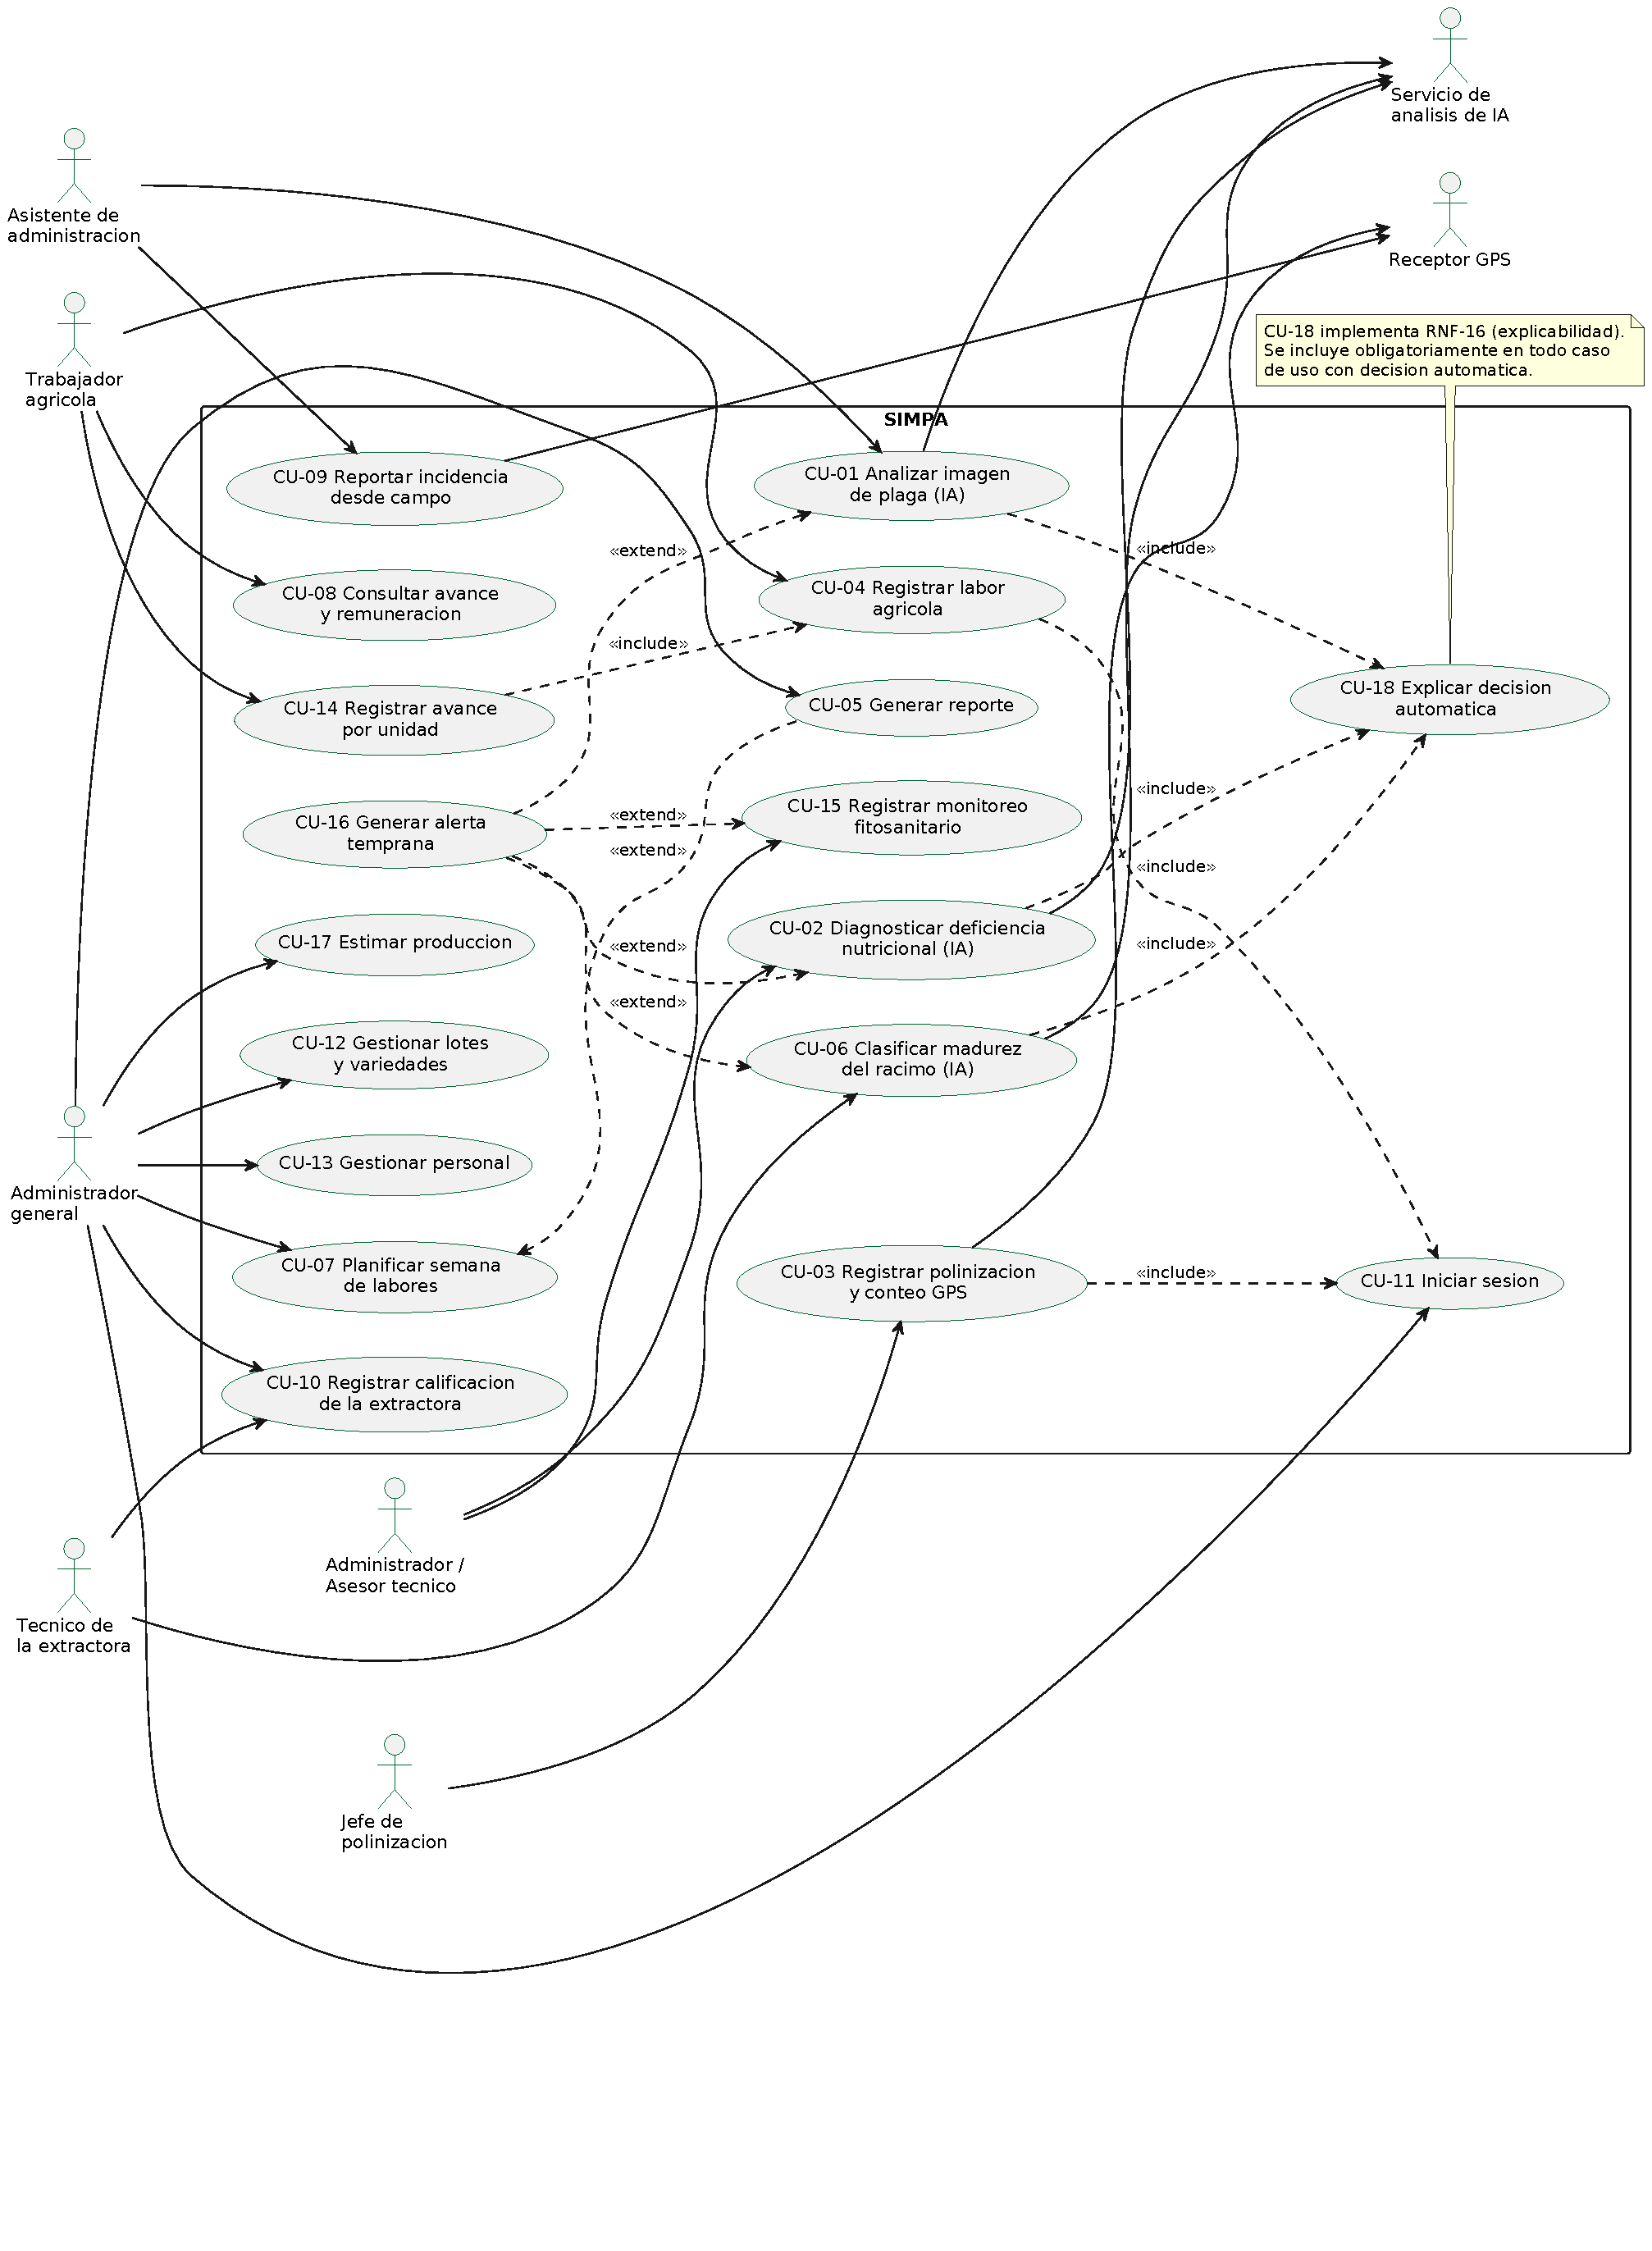
\includegraphics[width=0.91\textwidth]{img/casos_uso_general}
\caption{Diagrama general de casos de uso del SIMPA, con los ocho actores y el límite del sistema.}
\label{fig:cu_general}
\end{figure}

\noindent\textbf{Relaciones de inclusión y extensión.} \id{CU-14} incluye a \id{CU-04}, dado que el
registro de avance presupone una labor registrada. \id{CU-04} y \id{CU-03} incluyen a \id{CU-11},
por requerir sesión autenticada. Los tres casos de uso con decisión automática ---\id{CU-01},
\id{CU-02} y \id{CU-06}--- incluyen obligatoriamente a \id{CU-18}, que materializa el requisito de
explicabilidad \id{RNF-16}: no existe decisión automática sin explicación asociada. \id{CU-16}
extiende a los casos de diagnóstico y de monitoreo, puesto que la alerta se genera únicamente si el
resultado es positivo.

% ---------------------------------------------------------------------
\subsection{Especificación textual de los casos de uso}

Se especifican diez casos de uso, correspondientes a la totalidad de los requisitos funcionales de
prioridad \emph{Must}. Cada especificación incluye actores, precondiciones, postcondiciones, flujo
principal, al menos un flujo alternativo y al menos una excepción.

% --- CU-01
\begin{longtable}{|L{3.4cm}|L{12.0cm}|}
\hline
\rowcolor{grisclaro}\multicolumn{2}{|l|}{\textbf{CU-01 --- Analizar imagen para detectar plaga o enfermedad}}\\
\hline
\textbf{Requisitos} & \id{RF-07}, \id{RF-09}, \id{RF-12}, \id{RNF-16} \\ \hline
\textbf{Actores} & Primario: técnico fitosanitario / asistente de administración. Secundario: servicio de análisis de IA. \\ \hline
\textbf{Precondición} & Persona usuaria autenticada; lote seleccionado; cámara disponible. \\ \hline
\textbf{Postcondición} & El diagnóstico y su explicación quedan registrados y asociados al lote y a la fecha. \\ \hline
\textbf{Flujo principal} & 1. La persona usuaria selecciona el lote y la opción \emph{Analizar imagen}. \newline 2. Captura la fotografía de la palma o de la hoja. \newline 3. El sistema valida la calidad de la imagen. \newline 4. El sistema envía la imagen al servicio de IA con los parámetros de la variedad del lote. \newline 5. El servicio devuelve la clase de afectación, el nivel de confianza y el rasgo visual determinante. \newline 6. El sistema genera la explicación conforme a \id{RNF-16}. \newline 7. El sistema muestra el resultado, la explicación y la recomendación de control, y registra el diagnóstico. \\ \hline
\textbf{Flujo alternativo A} & \emph{Sin conectividad.} En el paso 4 el sistema almacena la imagen localmente y encola el análisis; al restablecerse la conexión lo ejecuta y notifica el resultado (\id{RNF-11}). \\ \hline
\textbf{Flujo alternativo B} & \emph{Confianza insuficiente.} Si el nivel de confianza es inferior al umbral configurado, el sistema no emite clasificación: informa que el resultado no es concluyente y sugiere repetir la captura o consultar a la asesoría técnica. \\ \hline
\textbf{Excepción E1} & Imagen de calidad insuficiente: el sistema solicita repetir la captura indicando el defecto detectado. \\ \hline
\textbf{Excepción E2} & Servicio de IA no disponible: el análisis queda en estado pendiente y la persona usuaria es notificada. \\ \hline
\textbf{Extensión} & Si el resultado es positivo, se ejecuta \id{CU-16} (generar alerta temprana). \\ \hline
\caption{CU-01 --- Analizar imagen para detectar plaga o enfermedad}
\end{longtable}

% --- CU-02
\begin{longtable}{|L{3.4cm}|L{12.0cm}|}
\hline
\rowcolor{grisclaro}\multicolumn{2}{|l|}{\textbf{CU-02 --- Diagnosticar deficiencia nutricional por imagen}}\\
\hline
\textbf{Requisitos} & \id{RF-08}, \id{RF-11}, \id{RNF-16} \\ \hline
\textbf{Actores} & Primario: administrador / asesor técnico. Secundario: servicio de análisis de IA. \\ \hline
\textbf{Precondición} & Persona usuaria autenticada; lote seleccionado con variedad asignada. \\ \hline
\textbf{Postcondición} & El diagnóstico nutricional y su recomendación quedan registrados en el historial del lote. \\ \hline
\textbf{Flujo principal} & 1. La persona usuaria selecciona \emph{Diagnóstico nutricional} y el lote. \newline 2. Captura la fotografía de la hoja. \newline 3. El sistema valida la imagen y la envía al servicio de IA. \newline 4. El servicio estima el elemento deficiente. \newline 5. El sistema genera una explicación de tipo causal, indicando qué signo foliar sustenta la estimación. \newline 6. El sistema muestra la deficiencia, la recomendación de fertilización y la explicación, y registra el diagnóstico. \\ \hline
\textbf{Flujo alternativo A} & La persona usuaria adjunta una imagen existente de la galería en lugar de capturarla. \\ \hline
\textbf{Flujo alternativo B} & \emph{Contraste con análisis de laboratorio.} Si el lote tiene un análisis de suelo o foliar registrado (\id{RF-11}), el sistema contrasta la estimación con los valores medidos y señala la discrepancia si la hubiere. \\ \hline
\textbf{Excepción E1} & Imagen no válida: el sistema solicita repetir la captura. \\ \hline
\textbf{Excepción E2} & Lote sin variedad asignada: el sistema advierte que la estimación puede no ser aplicable y solicita completar el dato. \\ \hline
\textbf{Extensión} & Si la deficiencia estimada es severa, se ejecuta \id{CU-16}. \\ \hline
\caption{CU-02 --- Diagnosticar deficiencia nutricional por imagen}
\end{longtable}

% --- CU-03
\begin{longtable}{|L{3.4cm}|L{12.0cm}|}
\hline
\rowcolor{grisclaro}\multicolumn{2}{|l|}{\textbf{CU-03 --- Registrar polinización y conteo georreferenciado}}\\
\hline
\textbf{Requisitos} & \id{RF-13}, \id{RF-14}, \id{RNF-05}, \id{RNF-12}, \id{RL-03} \\ \hline
\textbf{Actores} & Primario: polinizador. Secundario: receptor GPS. \\ \hline
\textbf{Precondición} & Lote en etapa de polinización; sesión iniciada; consentimiento de geolocalización vigente. \\ \hline
\textbf{Postcondición} & La polinización y el conteo diario quedan registrados por persona, lote y fecha, sin ingreso manual planta por planta. \\ \hline
\textbf{Flujo principal} & 1. El polinizador inicia la jornada en el lote. \newline 2. El sistema verifica la vigencia del consentimiento de geolocalización. \newline 3. El sistema activa el rastreo con período de muestreo de 30 s. \newline 4. Durante la jornada, el sistema almacena las marcaciones georreferenciadas. \newline 5. El polinizador registra el estado de la antesis y la verificación visual. \newline 6. Al cierre, el sistema calcula el número de flores polinizadas a partir de las marcaciones. \newline 7. El sistema almacena el registro y muestra el total a la persona trabajadora. \\ \hline
\textbf{Flujo alternativo A} & \emph{Consentimiento revocado.} Si el consentimiento no está vigente, el sistema no activa el rastreo y habilita el registro manual del número de flores, sin penalización para la persona trabajadora (\id{RL-03}). \\ \hline
\textbf{Flujo alternativo B} & \emph{Sin conectividad.} Las marcaciones se almacenan localmente y se sincronizan al reconectar (\id{RNF-11}). \\ \hline
\textbf{Excepción E1} & Precisión GPS superior a 10 m: el sistema conserva el dato marcándolo como de precisión degradada y advierte a la persona usuaria, sin descartar la jornada (\id{RNF-12}). \\ \hline
\textbf{Excepción E2} & Pérdida total de señal GPS durante la jornada: el sistema conserva el tramo registrado y solicita completar el conteo de forma manual para el tramo faltante. \\ \hline
\caption{CU-03 --- Registrar polinización y conteo georreferenciado}
\end{longtable}

% --- CU-04
\begin{longtable}{|L{3.4cm}|L{12.0cm}|}
\hline
\rowcolor{grisclaro}\multicolumn{2}{|l|}{\textbf{CU-04 --- Registrar labor agrícola}}\\
\hline
\textbf{Requisitos} & \id{RF-04}, \id{RF-28}, \id{RF-35} \\ \hline
\textbf{Actores} & Primario: trabajador agrícola. Alternativo: jefe de campo (registro delegado). \\ \hline
\textbf{Precondición} & Lote y persona trabajadora registrados; persona usuaria autenticada. \\ \hline
\textbf{Postcondición} & La labor y su avance quedan en el historial del lote y computan para el cumplimiento del plan semanal. \\ \hline
\textbf{Flujo principal} & 1. La persona usuaria selecciona el lote y el tipo de labor. \newline 2. Ingresa la cantidad ejecutada en la unidad correspondiente. \newline 3. El sistema valida que la unidad corresponda al tipo de labor. \newline 4. El sistema registra la labor asociada al lote, la fecha y la persona responsable. \newline 5. El sistema actualiza el avance acumulado del período y el cumplimiento de la meta semanal. \\ \hline
\textbf{Flujo alternativo A} & \emph{Registro delegado.} Si la persona trabajadora no dispone de dispositivo propio, el jefe de campo registra el avance en su nombre; el sistema conserva en bitácora la identidad de quien efectuó el registro (\id{RF-35}, \id{RD-10}). \\ \hline
\textbf{Flujo alternativo B} & \emph{Sin conectividad.} La labor se almacena localmente y se sincroniza al reconectar. \\ \hline
\textbf{Excepción E1} & Datos incompletos: el sistema impide guardar y señala los campos faltantes. \\ \hline
\textbf{Excepción E2} & Unidad incompatible con el tipo de labor: el sistema rechaza el registro e indica la unidad esperada. \\ \hline
\caption{CU-04 --- Registrar labor agrícola}
\end{longtable}

% --- CU-05
\begin{longtable}{|L{3.4cm}|L{12.0cm}|}
\hline
\rowcolor{grisclaro}\multicolumn{2}{|l|}{\textbf{CU-05 --- Generar reporte}}\\
\hline
\textbf{Requisitos} & \id{RF-19}, \id{RF-26} \\ \hline
\textbf{Actores} & Primario: administrador general. \\ \hline
\textbf{Precondición} & Existen registros en el período seleccionado. \\ \hline
\textbf{Postcondición} & El reporte queda disponible para consulta o exportación. \\ \hline
\textbf{Flujo principal} & 1. La persona administradora selecciona el tipo de reporte y el período. \newline 2. El sistema consolida labores, avance, producción y alertas del período. \newline 3. El sistema genera y presenta el reporte. \newline 4. La persona administradora lo consulta o lo exporta a PDF o a hoja de cálculo. \\ \hline
\textbf{Flujo alternativo A} & Filtrado por lote, por equipo o por persona trabajadora. \\ \hline
\textbf{Flujo alternativo B} & \emph{Reporte de cumplimiento semanal.} El sistema contrasta el plan de la semana con lo ejecutado y destaca las metas no alcanzadas y su remanente. \\ \hline
\textbf{Excepción E1} & Sin registros en el período: el sistema informa la ausencia de datos y propone un período alternativo con información disponible. \\ \hline
\caption{CU-05 --- Generar reporte}
\end{longtable}

% --- CU-06
\begin{longtable}{|L{3.4cm}|L{12.0cm}|}
\hline
\rowcolor{grisclaro}\multicolumn{2}{|l|}{\textbf{CU-06 --- Clasificar la madurez del racimo}}\\
\hline
\textbf{Requisitos} & \id{RF-21}, \id{RF-22}, \id{RD-07}, \id{RD-08}, \id{RNF-01}, \id{RNF-16} \\ \hline
\textbf{Actores} & Primario: cosechador / técnico de la extractora. Secundario: servicio de análisis de IA. \\ \hline
\textbf{Precondición} & Lote con variedad asignada; persona usuaria autenticada. \\ \hline
\textbf{Postcondición} & La clasificación queda asociada al racimo, al lote y a la fecha, y actualiza el porcentaje estimado de fruta verde del lote. \\ \hline
\textbf{Flujo principal} & 1. La persona usuaria selecciona el lote y la opción \emph{Clasificar racimo}. \newline 2. El sistema recupera el umbral de desprendimiento de la variedad del lote. \newline 3. La persona usuaria captura la fotografía de la parte basal del racimo. \newline 4. El servicio de IA cuenta los frutos desprendidos, sin emplear el color como criterio (\id{RD-07}). \newline 5. El sistema compara el conteo con el umbral de la variedad y determina el estado. \newline 6. El sistema genera una explicación por contraste, indicando el conteo obtenido y el umbral aplicable. \newline 7. El sistema registra la clasificación y actualiza el porcentaje de fruta verde del lote. \\ \hline
\textbf{Flujo alternativo A} & \emph{Verificación previa al despacho.} La persona usuaria solicita el porcentaje estimado de fruta verde del lote; si alcanza o supera el umbral de penalización, el sistema emite alerta preventiva y desaconseja el despacho (\id{RF-22}). \\ \hline
\textbf{Flujo alternativo B} & \emph{Sobremadurez.} Si el conteo excede ampliamente el umbral, el sistema clasifica el racimo como sobremaduro y advierte sobre el incremento de acidez. \\ \hline
\textbf{Excepción E1} & Lote sin variedad asignada: el sistema no clasifica y solicita completar el dato, dado que el umbral depende de la variedad. \\ \hline
\textbf{Excepción E2} & Parte basal no visible en la imagen: el sistema solicita repetir la captura indicando el encuadre requerido. \\ \hline
\caption{CU-06 --- Clasificar la madurez del racimo}
\end{longtable}

% --- CU-07
\begin{longtable}{|L{3.4cm}|L{12.0cm}|}
\hline
\rowcolor{grisclaro}\multicolumn{2}{|l|}{\textbf{CU-07 --- Planificar la semana de labores}}\\
\hline
\textbf{Requisitos} & \id{RF-26}, \id{RF-27}, \id{RF-34}, \id{RF-37} a \id{RF-39} \\ \hline
\textbf{Actores} & Primario: administrador general. \\ \hline
\textbf{Precondición} & Lotes y tipos de labor registrados. \\ \hline
\textbf{Postcondición} & El plan de la semana queda publicado y disponible para el seguimiento diario. \\ \hline
\textbf{Flujo principal} & 1. La persona administradora crea el plan de la semana. \newline 2. Para cada lote, define las labores previstas con su meta y unidad. \newline 3. El sistema incorpora automáticamente los remanentes arrastrados de la semana anterior. \newline 4. La persona administradora registra los insumos requeridos. \newline 5. El sistema publica el plan y lo hace visible al jefe de campo. \\ \hline
\textbf{Flujo alternativo A} & \emph{Cierre de semana.} Al cierre, el sistema calcula el cumplimiento de cada meta; si es parcial, genera el remanente como labor pendiente de la semana siguiente, vinculada a la de origen (\id{RF-27}). \\ \hline
\textbf{Flujo alternativo B} & Ajuste del plan durante la semana en curso, conservando la versión previa en bitácora. \\ \hline
\textbf{Flujo alternativo C} & \emph{Liquidación y aprobación.} Al cierre, el sistema genera la liquidación que contrasta cantidad presupuestada, cantidad ejecutada, tarifa y valor por grupo de labor, totaliza el gasto presupuestado frente al real, e incorpora las labores no presupuestadas en su grupo diferenciado (\id{RF-37}, \id{RF-38}). La persona administradora aprueba la liquidación y el período queda cerrado (\id{RF-39}). \\ \hline
\textbf{Excepción E1} & Meta expresada en unidad incompatible con el tipo de labor: el sistema rechaza la meta e indica la unidad esperada. \\ \hline
\textbf{Excepción E2} & Existe un plan publicado para la misma semana: el sistema advierte y solicita confirmación antes de sustituirlo. \\ \hline
\caption{CU-07 --- Planificar la semana de labores}
\end{longtable}

% --- CU-08
\begin{longtable}{|L{3.4cm}|L{12.0cm}|}
\hline
\rowcolor{grisclaro}\multicolumn{2}{|l|}{\textbf{CU-08 --- Consultar avance acumulado y remuneración estimada}}\\
\hline
\textbf{Requisitos} & \id{RF-29}, \id{RF-36}, \id{RL-04} \\ \hline
\textbf{Actores} & Primario: trabajador agrícola. \\ \hline
\textbf{Precondición} & Existen registros de avance de la persona trabajadora en el período. \\ \hline
\textbf{Postcondición} & Se presenta el consolidado del período, sin posibilidad de edición por parte de la persona trabajadora. \\ \hline
\textbf{Flujo principal} & 1. La persona trabajadora accede a \emph{Mi avance}. \newline 2. Selecciona el período (quincena en curso por defecto). \newline 3. El sistema agrega sus registros de avance por tipo de labor. \newline 4. El sistema obtiene del catálogo la tarifa vigente de cada tipo de labor a la fecha de cada registro y calcula la remuneración estimada correspondiente al trabajo por avance. \newline 5. El sistema presenta el desglose por labor y el total estimado. \\ \hline
\textbf{Flujo alternativo A} & \emph{Ejercicio del derecho de acceso.} La persona trabajadora solicita la exportación de sus datos personales; el sistema genera el archivo conforme al Art. 12 de la LOPDP (\id{RL-04}). \\ \hline
\textbf{Flujo alternativo B} & \emph{Discrepancia.} La persona trabajadora marca un registro como discrepante; el sistema notifica a la administración sin modificar el dato original, y la corrección se tramita mediante \id{RL-05}. \\ \hline
\textbf{Excepción E1} & Sin registros en el período: el sistema informa la ausencia de datos. \\ \hline
\textbf{Excepción E2} & La labor carece de tarifa vigente en el catálogo (\id{RF-36}) a la fecha del registro: el sistema muestra el avance en unidades, omite la estimación monetaria e indica que la tarifa no está vigente para esa fecha. \\ \hline
\caption{CU-08 --- Consultar avance acumulado y remuneración estimada}
\end{longtable}

% --- CU-09
\begin{longtable}{|L{3.4cm}|L{12.0cm}|}
\hline
\rowcolor{grisclaro}\multicolumn{2}{|l|}{\textbf{CU-09 --- Reportar incidencia desde el campo}}\\
\hline
\textbf{Requisitos} & \id{RF-30}, \id{RF-31}, \id{RF-12} \\ \hline
\textbf{Actores} & Primario: asistente de administración / trabajador agrícola. Secundario: receptor GPS. \\ \hline
\textbf{Precondición} & Persona usuaria autenticada; cámara y GPS disponibles. \\ \hline
\textbf{Postcondición} & La incidencia queda registrada con fotografía y coordenadas, e incorporada a la lista de pendientes de verificación. \\ \hline
\textbf{Flujo principal} & 1. La persona usuaria selecciona \emph{Reportar incidencia}. \newline 2. Captura la fotografía de la afectación. \newline 3. El sistema obtiene las coordenadas del punto. \newline 4. La persona usuaria selecciona el lote y describe la afectación. \newline 5. El sistema registra la incidencia georreferenciada. \newline 6. El sistema la incorpora a la lista de pendientes de la persona supervisora. \\ \hline
\textbf{Flujo alternativo A} & \emph{Análisis asistido.} La persona usuaria solicita el análisis de la fotografía; se ejecuta \id{CU-01} y el diagnóstico se asocia a la incidencia. \\ \hline
\textbf{Flujo alternativo B} & \emph{Verificación en visita.} La persona supervisora recorre su lista de pendientes, ubica la incidencia por sus coordenadas y la marca como verificada o descartada. \\ \hline
\textbf{Excepción E1} & GPS no disponible: el sistema registra la incidencia solicitando la selección manual del lote y la marca como de ubicación aproximada. \\ \hline
\textbf{Excepción E2} & Sin conectividad: la incidencia se encola y se sincroniza al reconectar, conservando el instante original de captura. \\ \hline
\caption{CU-09 --- Reportar incidencia desde el campo}
\end{longtable}

% --- CU-10
\begin{longtable}{|L{3.4cm}|L{12.0cm}|}
\hline
\rowcolor{grisclaro}\multicolumn{2}{|l|}{\textbf{CU-10 --- Registrar la calificación de la planta extractora}}\\
\hline
\textbf{Requisitos} & \id{RF-23}, \id{RF-24}, \id{RF-25}, \id{RF-33} \\ \hline
\textbf{Actores} & Primario: administrador general. \\ \hline
\textbf{Precondición} & Existe un despacho registrado con su fecha de corte. \\ \hline
\textbf{Postcondición} & La calificación queda asociada al lote de origen y disponible para el análisis de trazabilidad. \\ \hline
\textbf{Flujo principal} & 1. La persona administradora selecciona el despacho. \newline 2. Ingresa los datos del ticket de pesaje: peso bruto, tara y neto. \newline 3. Ingresa la calificación de calidad: tamaño del fruto, porcentaje de fruta verde, sobremadura, malformación y pedúnculo largo. \newline 4. El sistema calcula el intervalo entre el corte y la entrega. \newline 5. El sistema registra la calificación y la asocia al lote de origen. \\ \hline
\textbf{Flujo alternativo A} & \emph{Análisis de trazabilidad.} Ante una calificación desfavorable, la persona administradora consulta la cadena lote $\rightarrow$ fecha de corte $\rightarrow$ cuadrilla, y contrasta con las labores del período para distinguir si el origen está en la cosecha o en el manejo del cultivo (\id{RF-24}). \\ \hline
\textbf{Flujo alternativo B} & \emph{Ausencia de guía de remisión.} Si el despacho se registra sin número de guía, el sistema advierte antes del cierre (\id{RF-33}). \\ \hline
\textbf{Excepción E1} & El intervalo entre corte y entrega supera el valor recomendado para la variedad: el sistema registra la advertencia junto al despacho (\id{RF-25}). \\ \hline
\textbf{Excepción E2} & La suma de pesos es inconsistente (neto distinto de bruto menos tara): el sistema rechaza el registro e indica la inconsistencia. \\ \hline
\caption{CU-10 --- Registrar la calificación de la planta extractora}
\end{longtable}

% ---------------------------------------------------------------------
\subsection{Diagrama de clases refinado}

El modelo del dominio comprende veinticinco clases con atributos y operaciones. Incorpora tres
jerarquías de herencia (\id{Persona}--\id{Usuario} y la especialización de \id{Diagnostico} en sus
tres variantes), cuatro relaciones de composición y asociaciones con multiplicidad explícita. No
corresponde a un diseño de base de datos, sino al modelo conceptual del dominio del problema.

\begin{figure}[!htbp]
\centering
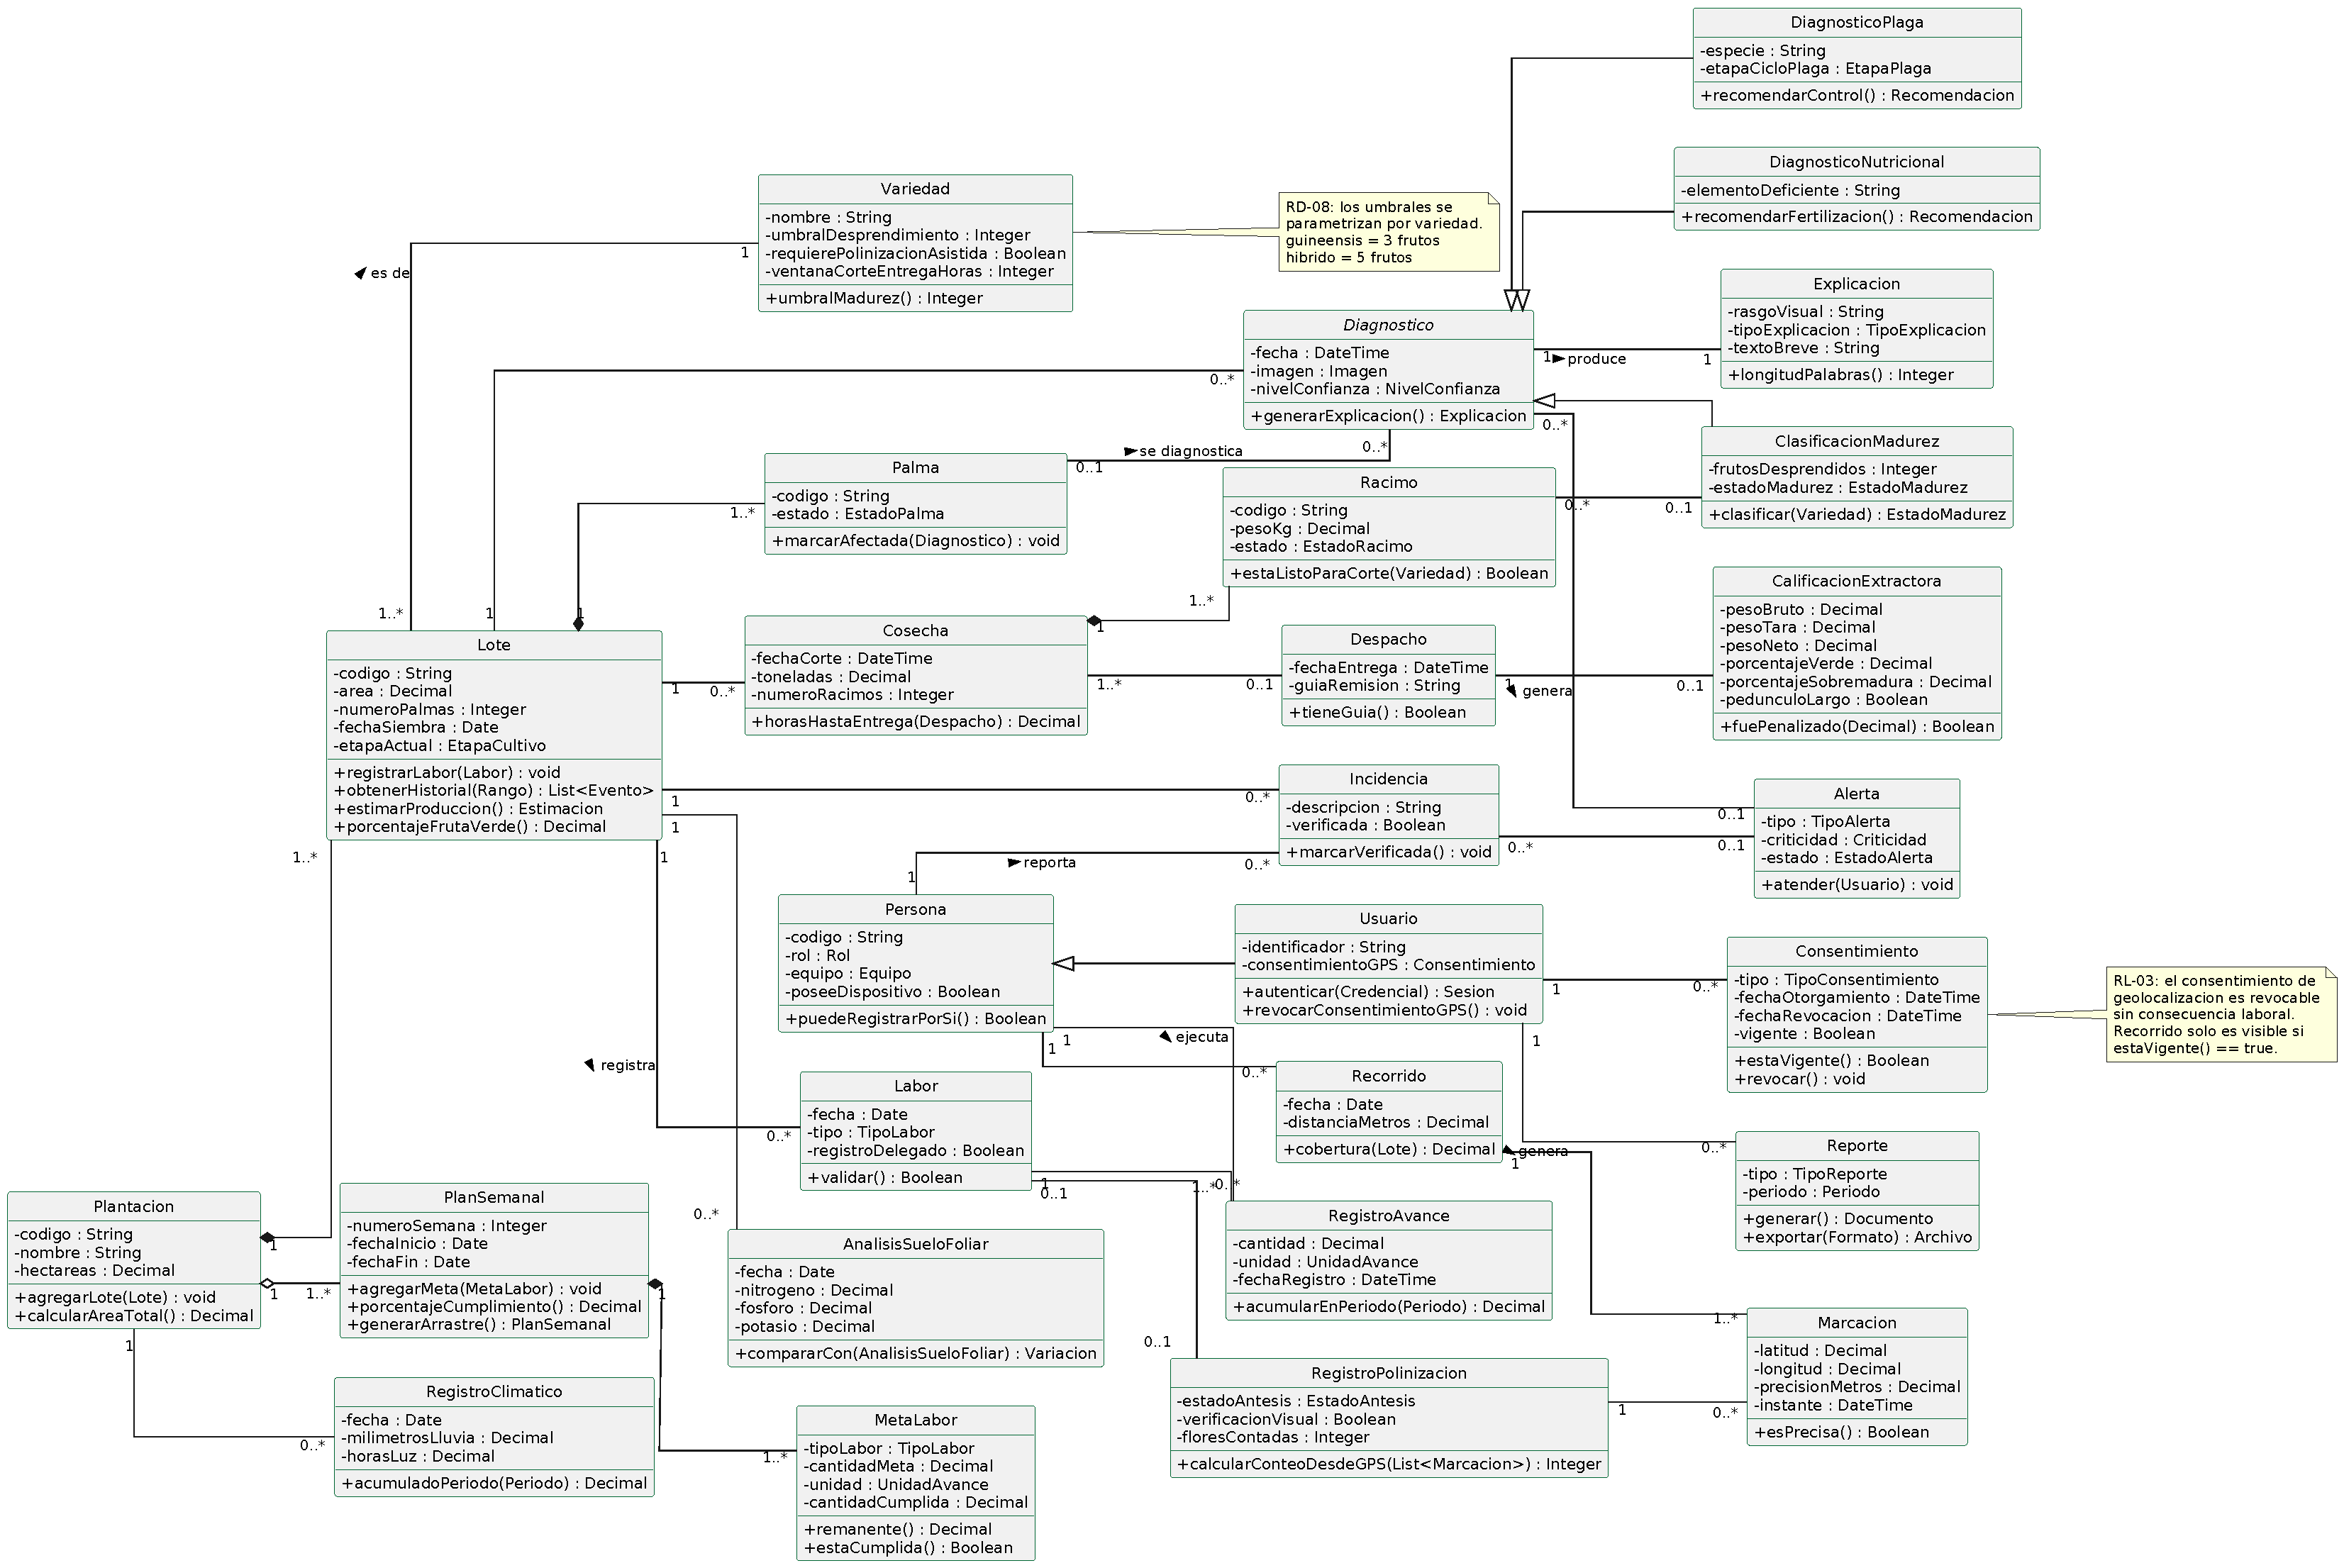
\includegraphics[width=1.0\textwidth]{img/clases_refinado}
\caption{Diagrama de clases refinado del SIMPA, con atributos y operaciones.}
\label{fig:clases}
\end{figure}

\noindent\textbf{Decisiones de modelado relevantes.} La clase \id{Consentimiento} se modela como
entidad de primer orden y no como atributo booleano de \id{Usuario}, porque el Art. 7 de la LOPDP
exige que el consentimiento sea específico por finalidad y revocable, lo que obliga a conservar su
historia. La clase \id{Variedad} concentra los umbrales de decisión ---desprendimiento, ventana
corte-entrega y necesidad de polinización asistida--- en lugar de fijarlos en la lógica de los
módulos de IA, conforme a \id{RD-08}. La clase \id{Explicacion} se asocia de forma obligatoria a
\id{Diagnostico} con multiplicidad 1:1, de modo que el modelo impide estructuralmente la existencia
de una decisión automática sin explicación (\id{RNF-16}). La clase \id{RegistroAvance} se separa de
\id{Labor} porque una labor puede acumular avances de varias personas y días, patrón observado en
los documentos de planificación semanal (\id{EV-11}).

% ---------------------------------------------------------------------
\subsection{Diagramas de secuencia}

Se presentan los diagramas de secuencia de los tres casos de uso \emph{Must} de mayor complejidad
de interacción.

\begin{figure}[!htbp]
\centering
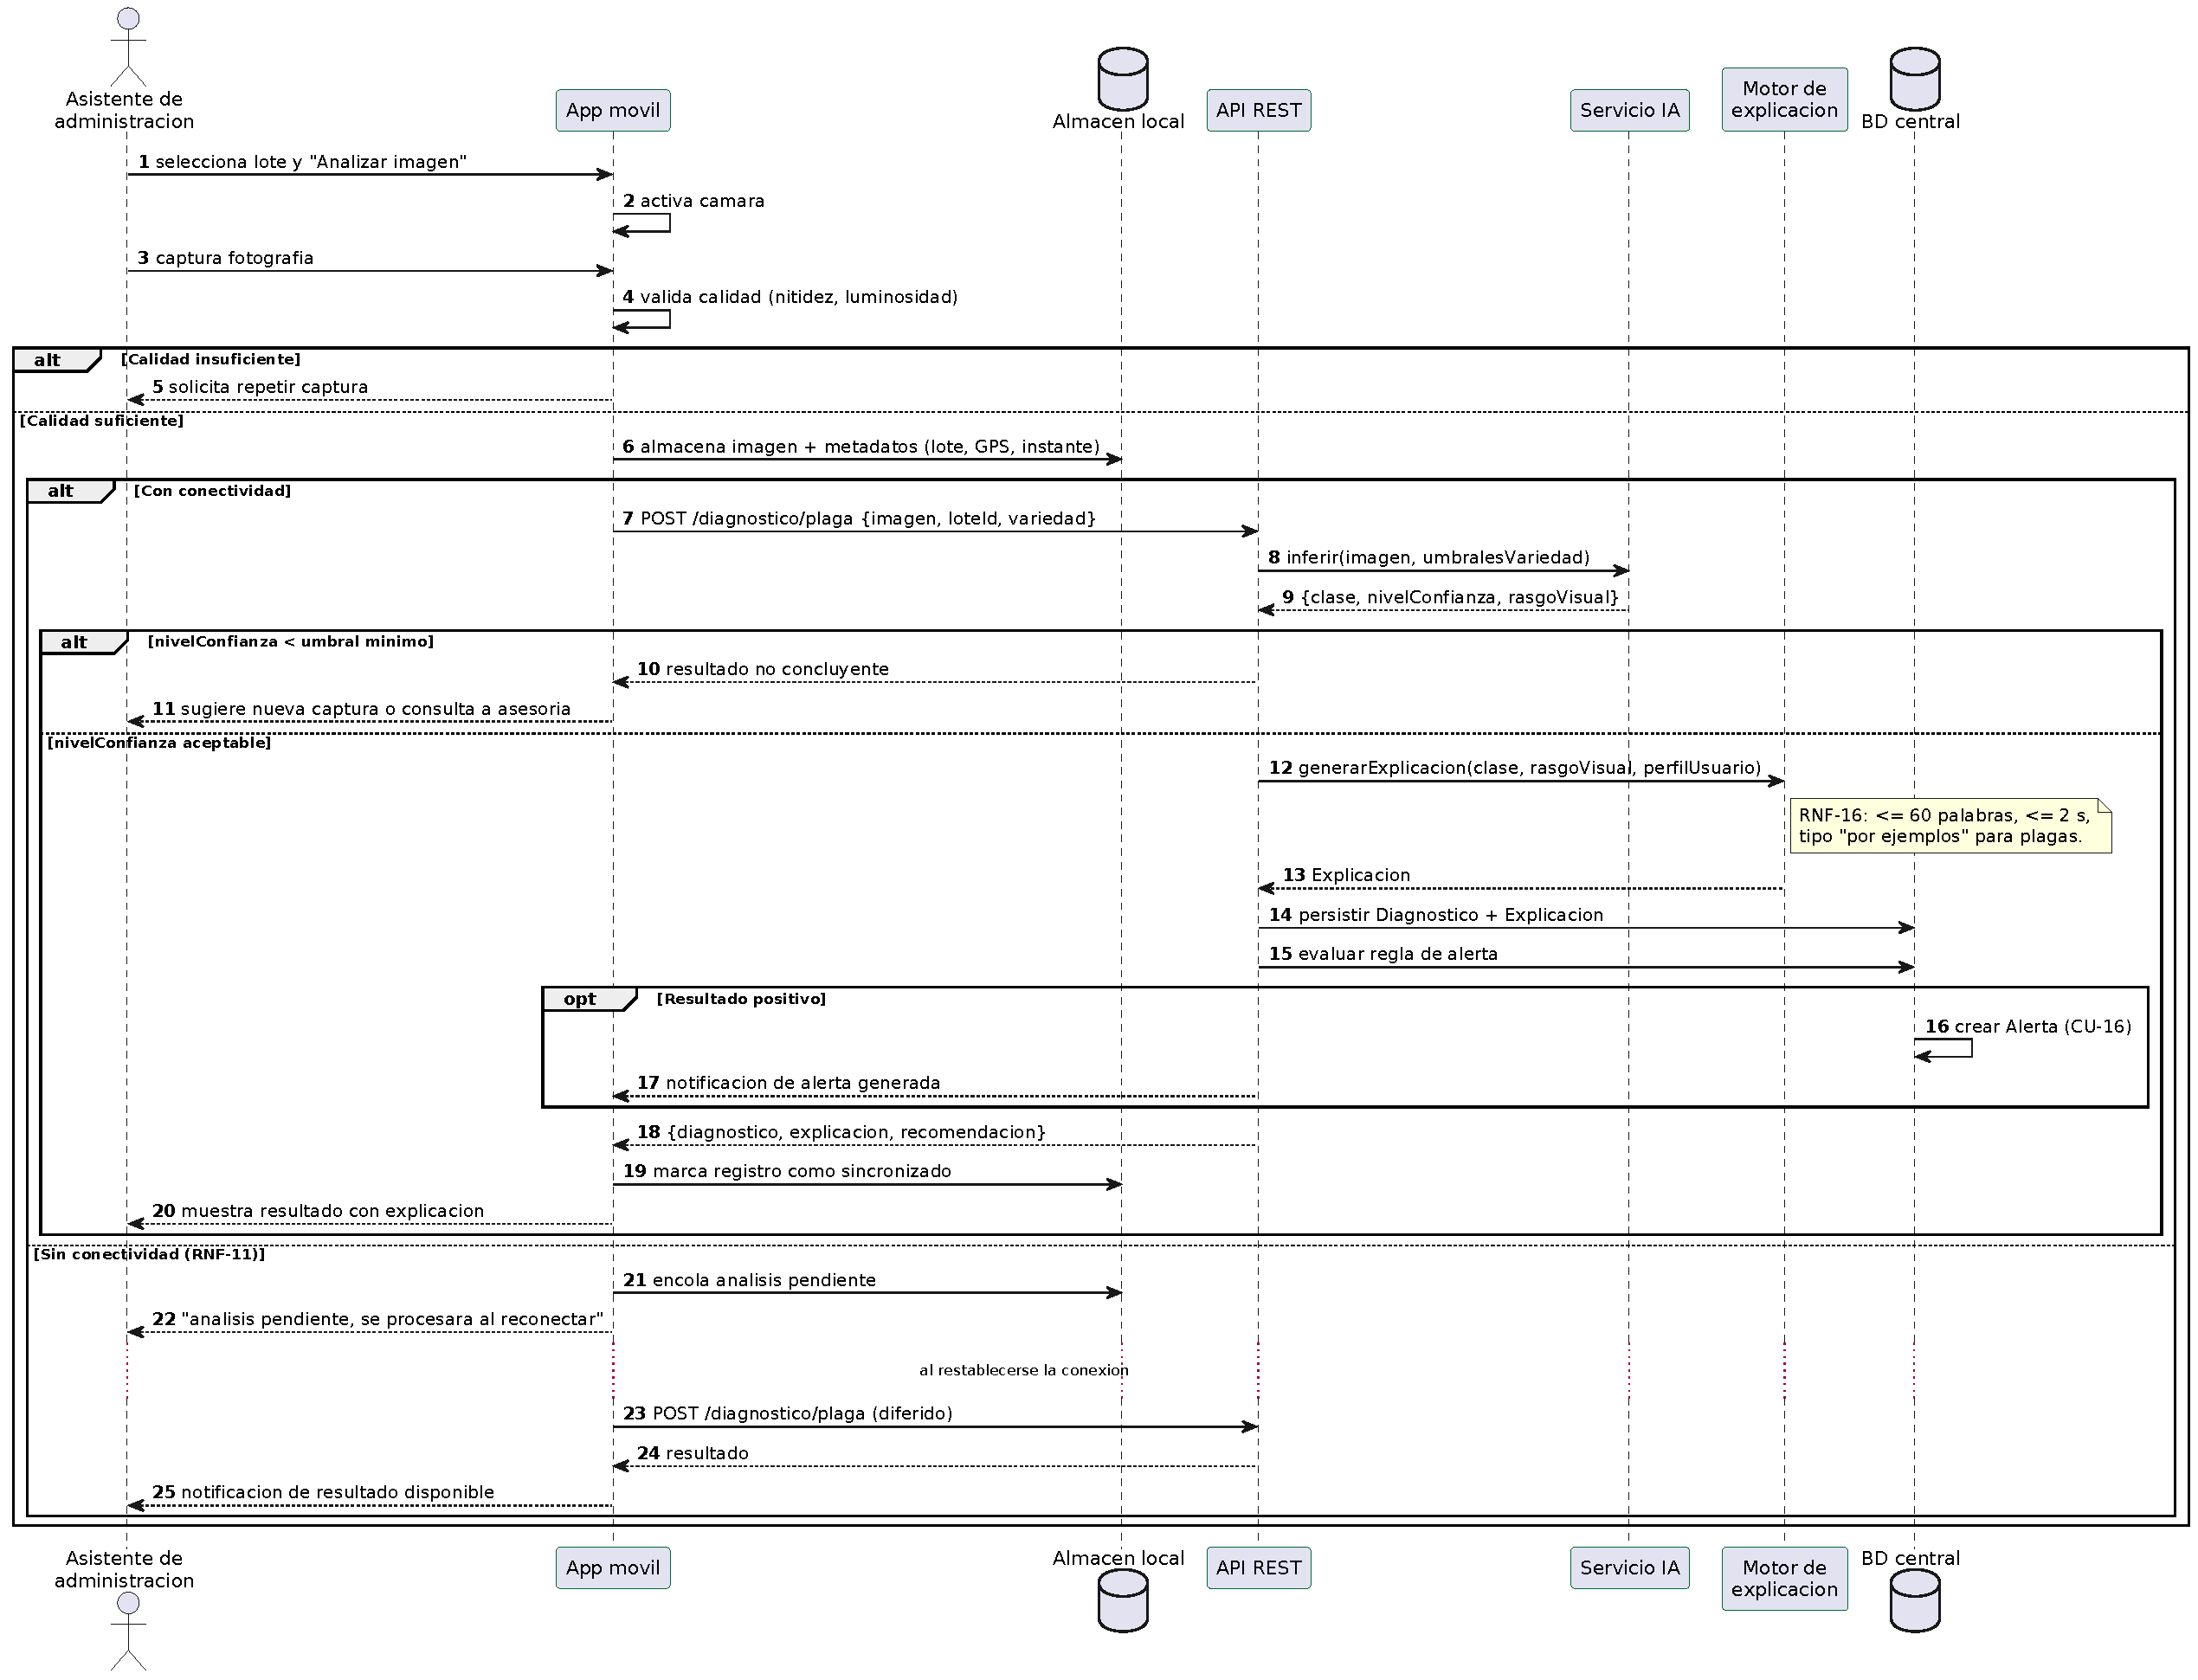
\includegraphics[width=1.0\textwidth]{img/secuencia_CU01}
\caption{Diagrama de secuencia del CU-01: análisis de imagen para detección de plaga, con las ramas de baja confianza y de operación sin conectividad.}
\label{fig:seq01}
\end{figure}

\begin{figure}[!htbp]
\centering
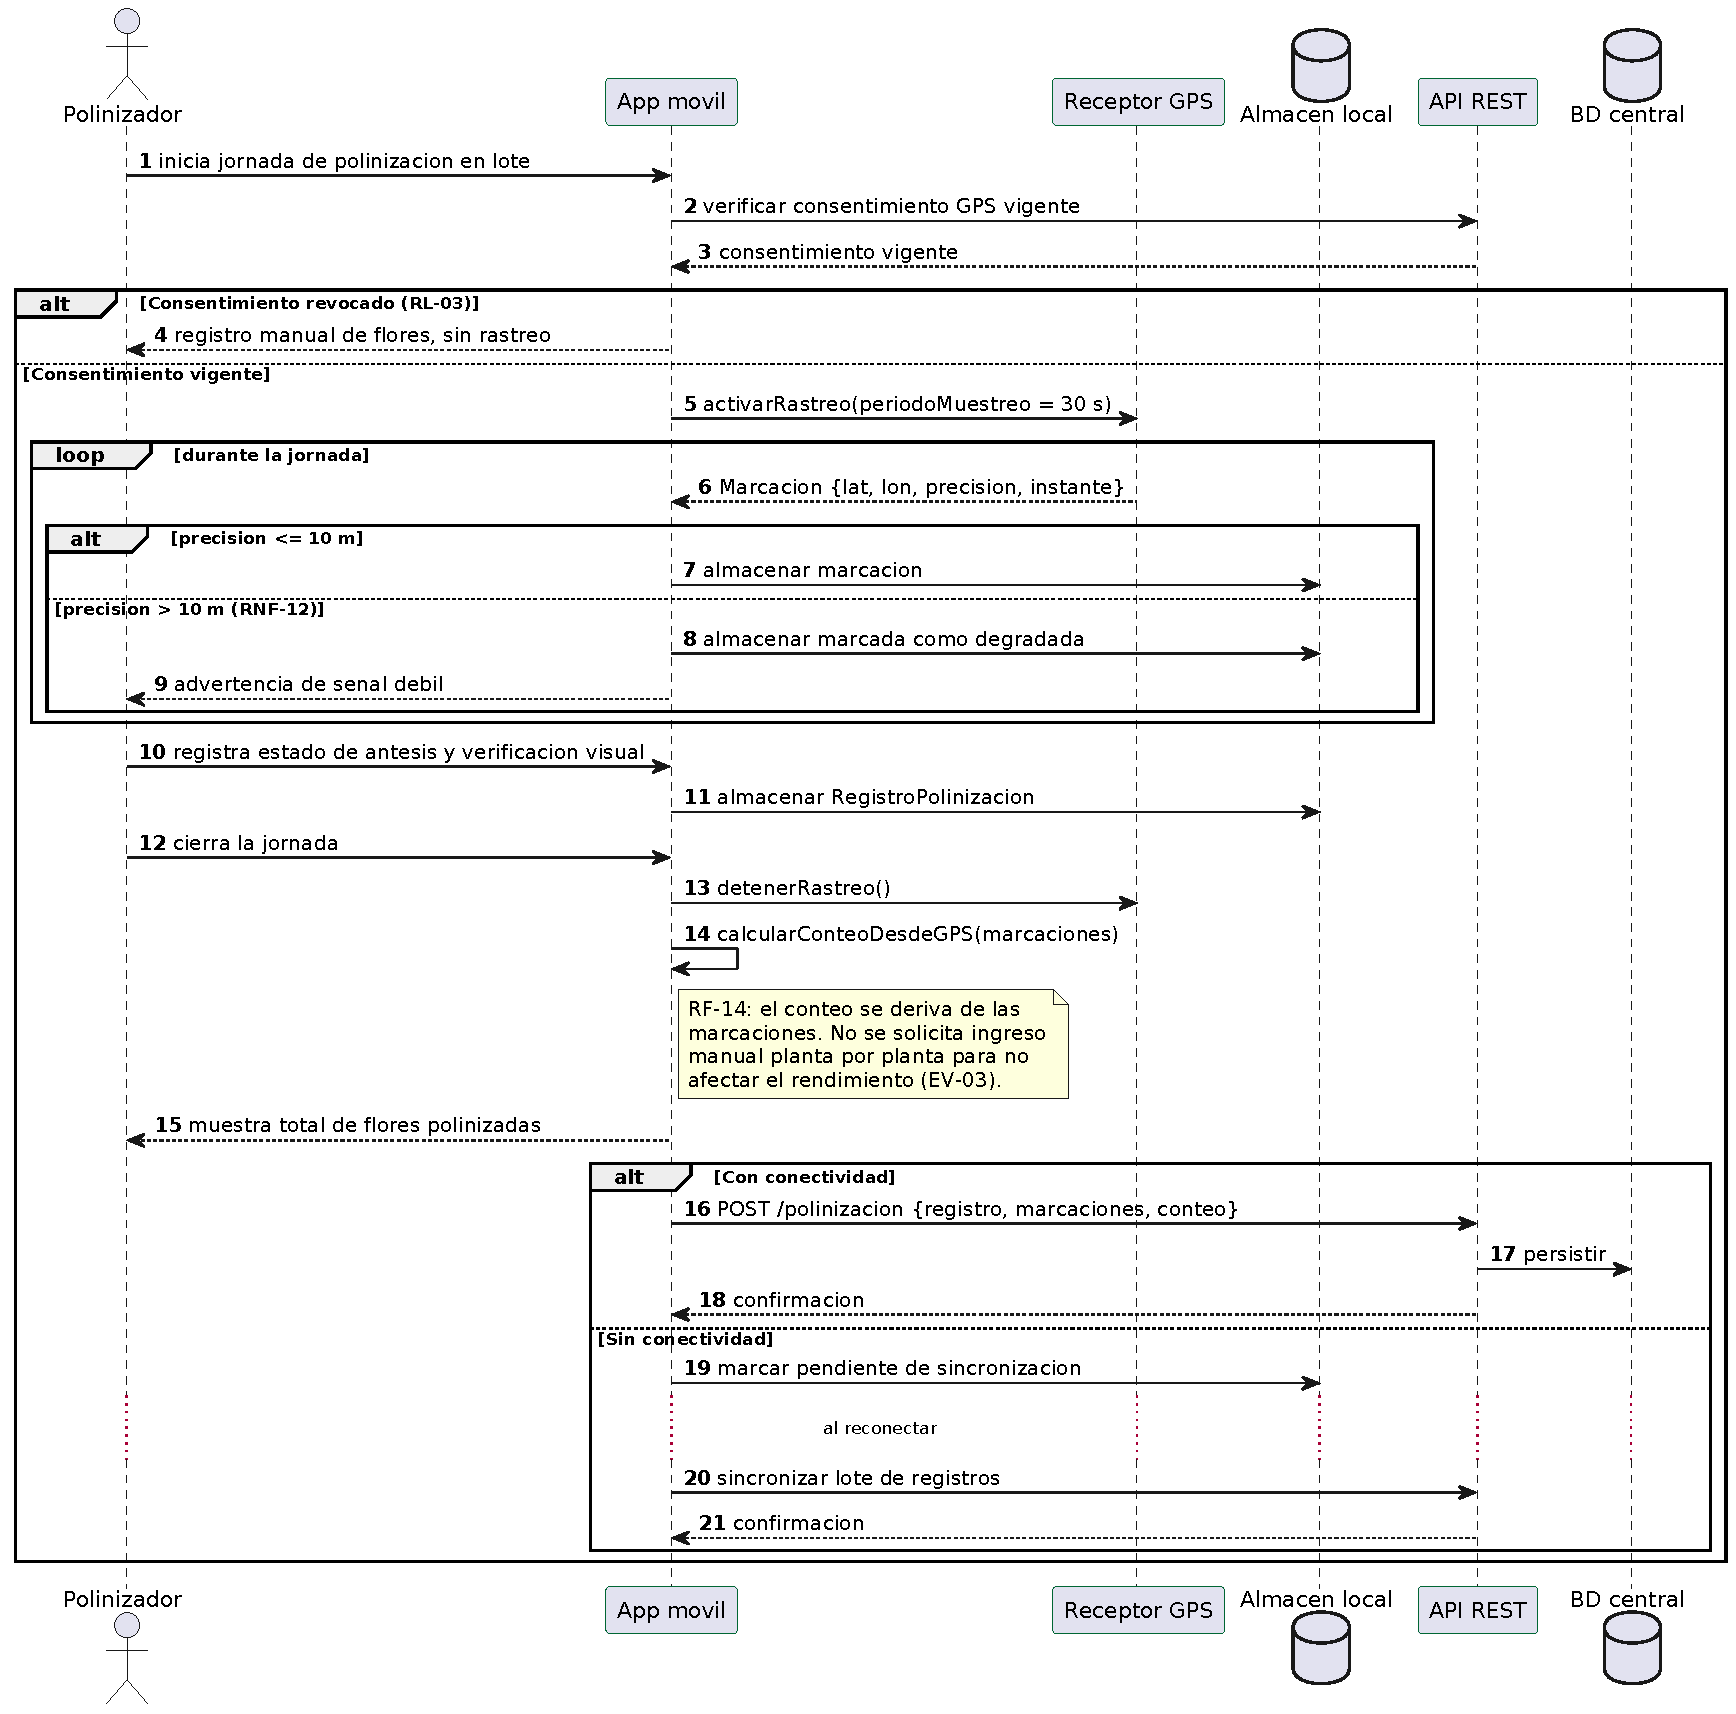
\includegraphics[width=1.0\textwidth]{img/secuencia_CU03}
\caption{Diagrama de secuencia del CU-03: registro de polinización y conteo georreferenciado, con verificación de consentimiento y manejo de precisión degradada.}
\label{fig:seq03}
\end{figure}

\begin{figure}[!htbp]
\centering
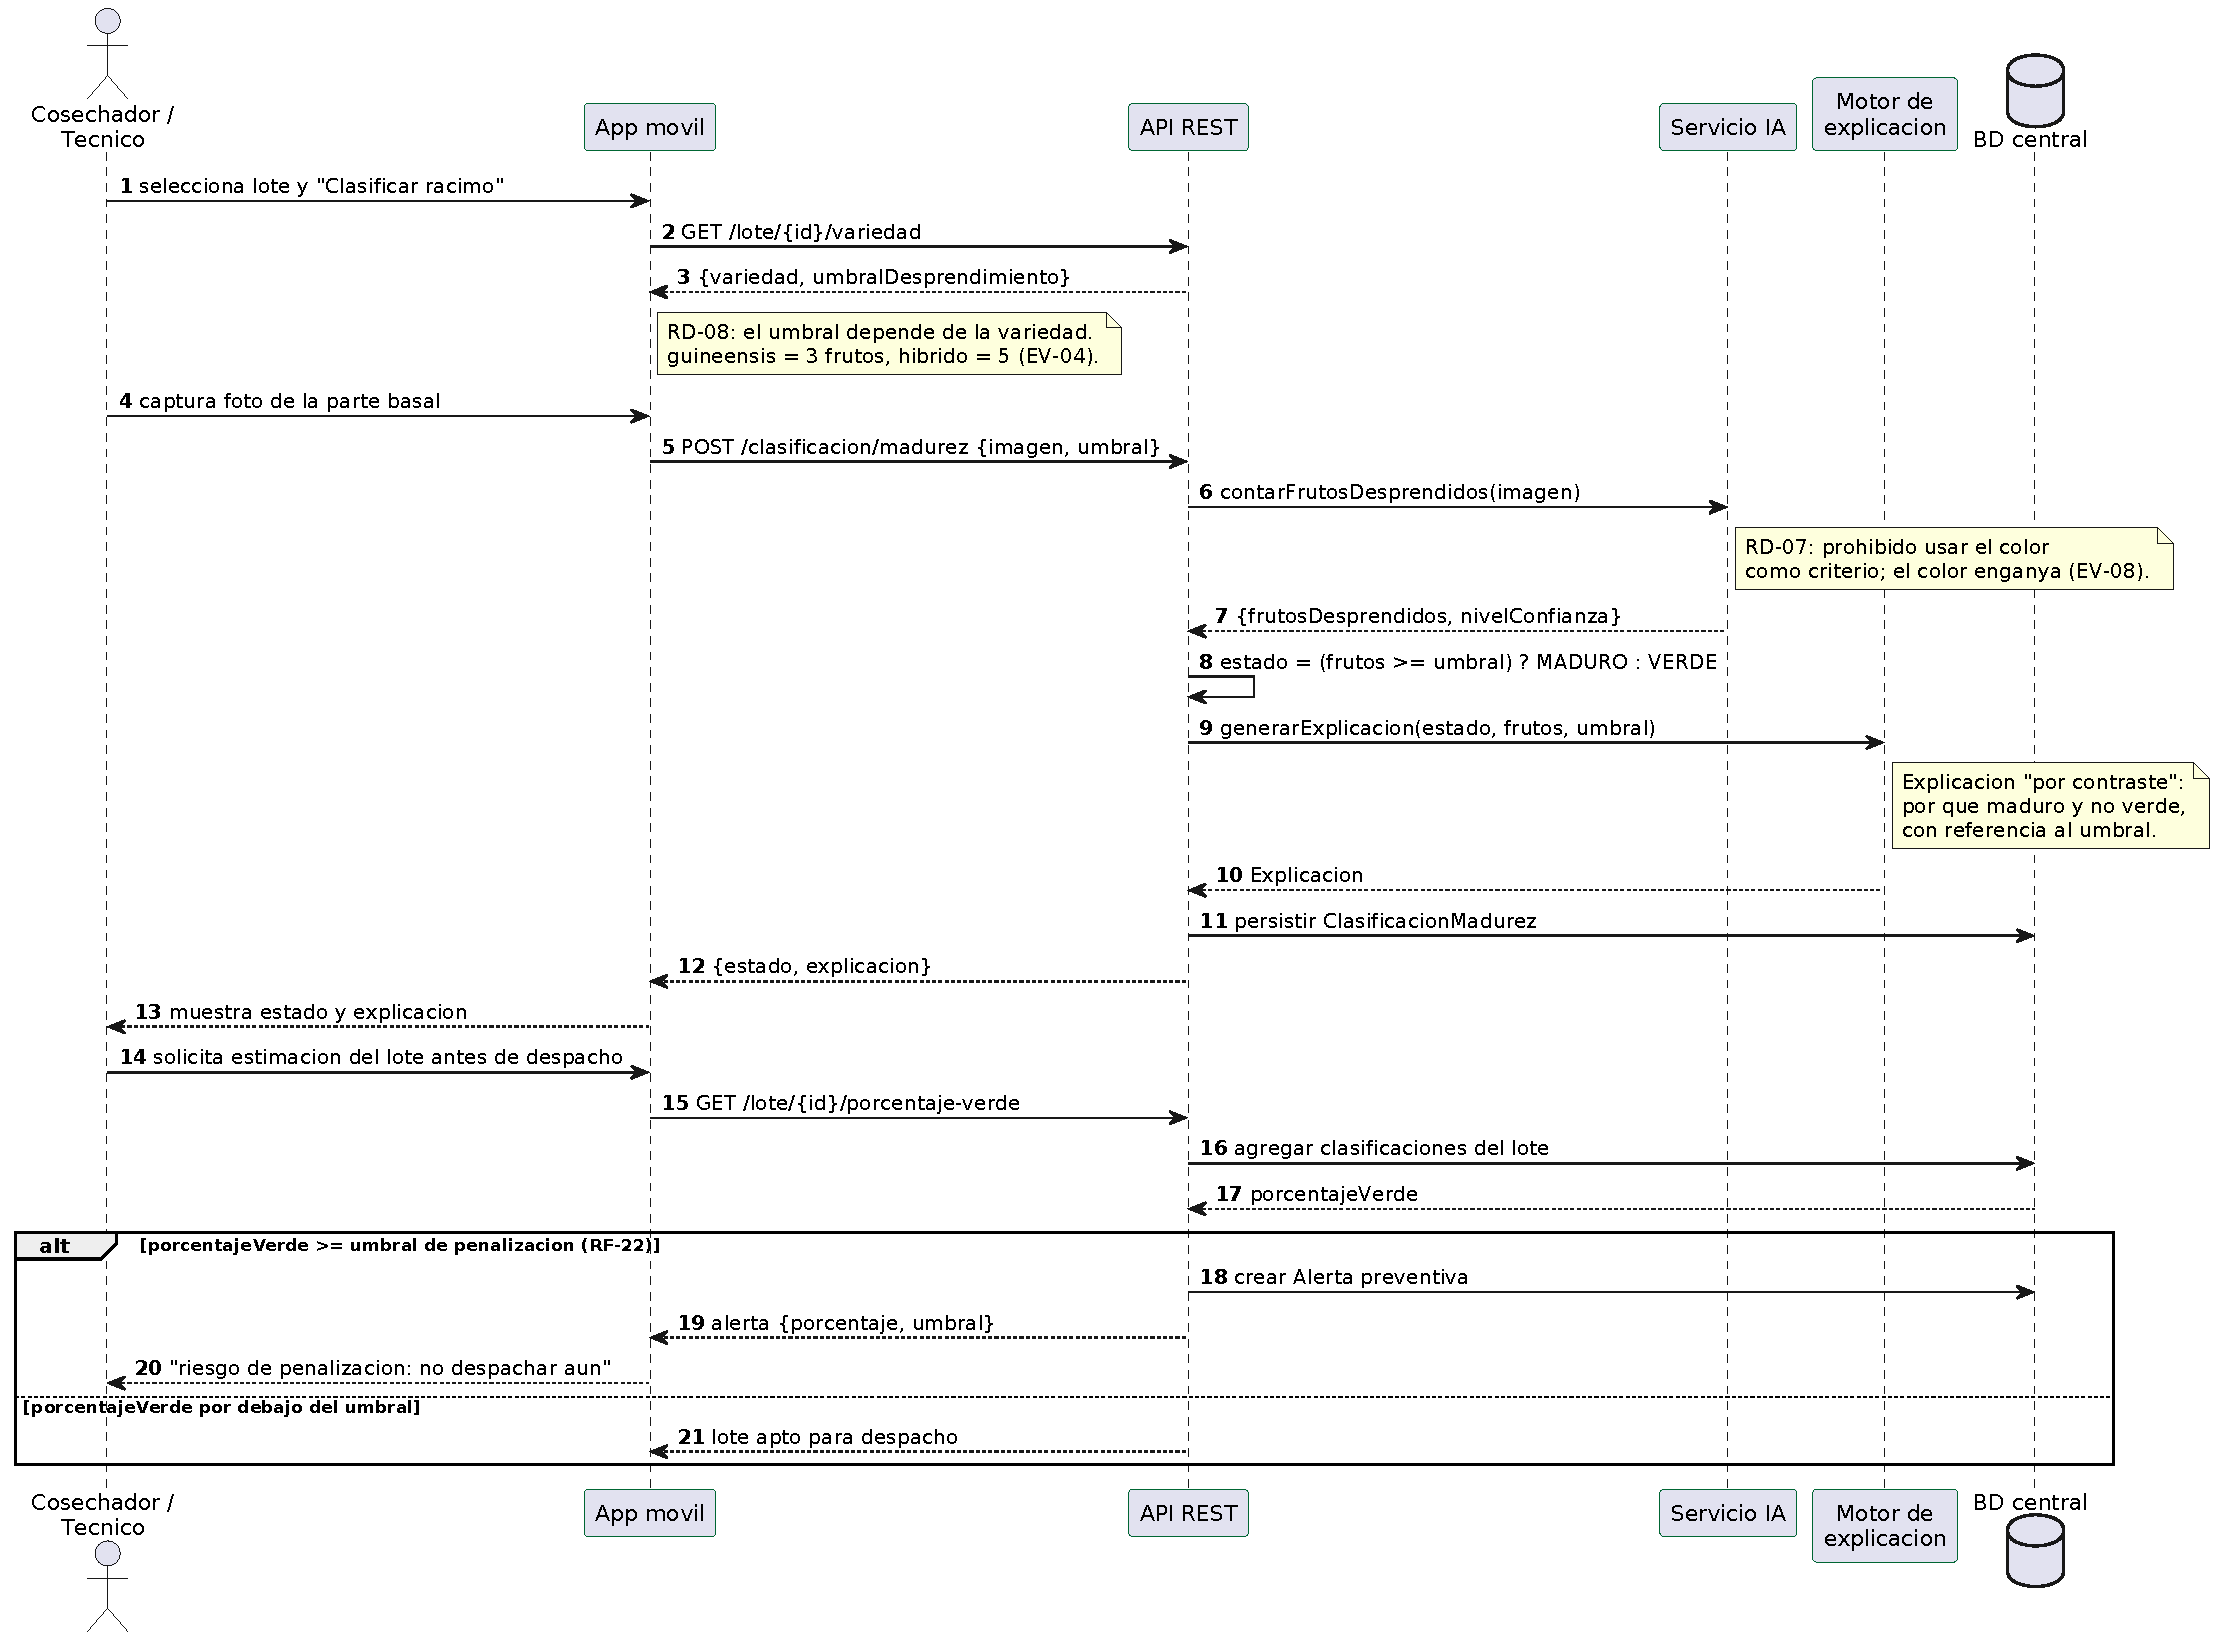
\includegraphics[width=1.0\textwidth]{img/secuencia_CU06}
\caption{Diagrama de secuencia del CU-06: clasificación de madurez del racimo y alerta preventiva de porcentaje de fruta verde.}
\label{fig:seq06}
\end{figure}

% ---------------------------------------------------------------------
\subsection{Diagrama de actividad}

El diagrama modela el ciclo semanal completo de planificación y ejecución, que constituye el proceso
central de la organización según los documentos operativos (\id{EV-11}). Incorpora la bifurcación
por disponibilidad de dispositivo (\id{RF-35}), la bifurcación por conectividad (\id{RNF-11}) y el
mecanismo de arrastre de labor incompleta (\id{RF-27}).

\begin{figure}[!htbp]
\centering
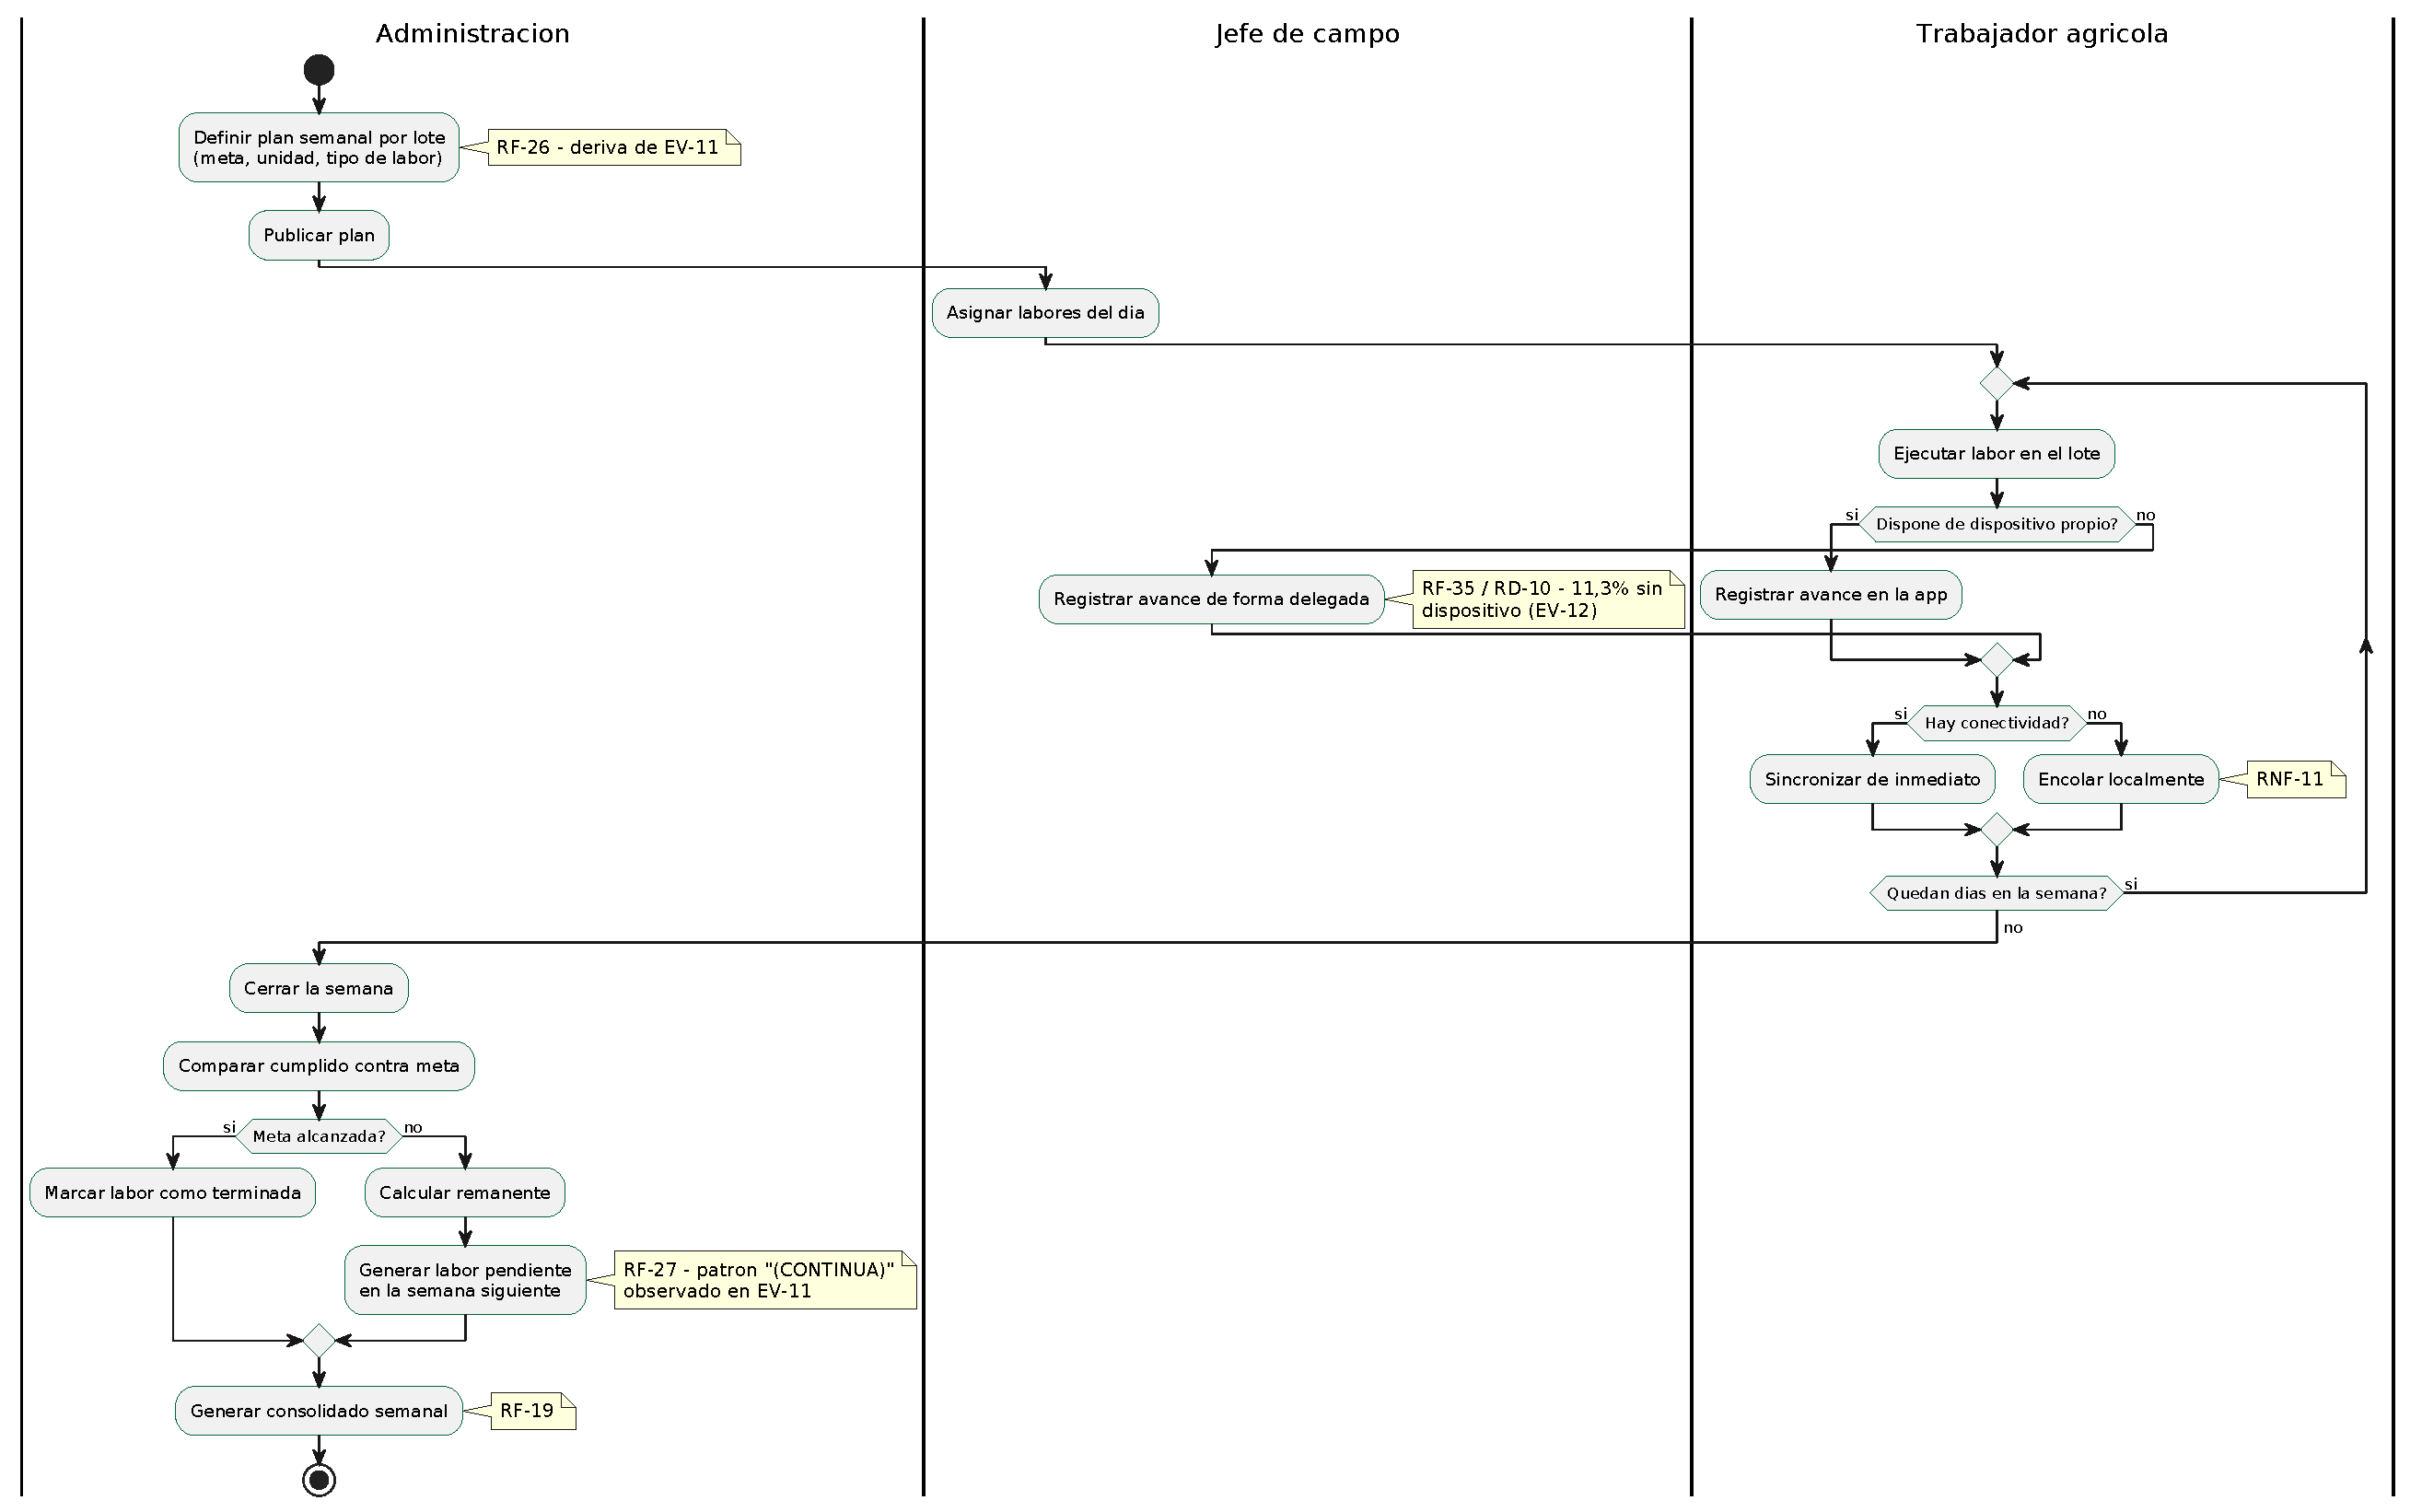
\includegraphics[width=1.0\textwidth]{img/actividad_ciclo_semanal}
\caption{Diagrama de actividad del ciclo semanal de planificación y ejecución de labores.}
\label{fig:actividad}
\end{figure}

% ---------------------------------------------------------------------
\subsection{Diagramas de estados}

Se modelan las dos entidades del dominio con ciclo de vida no trivial: el \textbf{racimo}, cuya
trayectoria determina el valor económico de la producción, y la \textbf{alerta}, cuyo ciclo refleja
la latencia real de verificación documentada en \id{EV-07}.

\begin{figure}[!htbp]
\centering
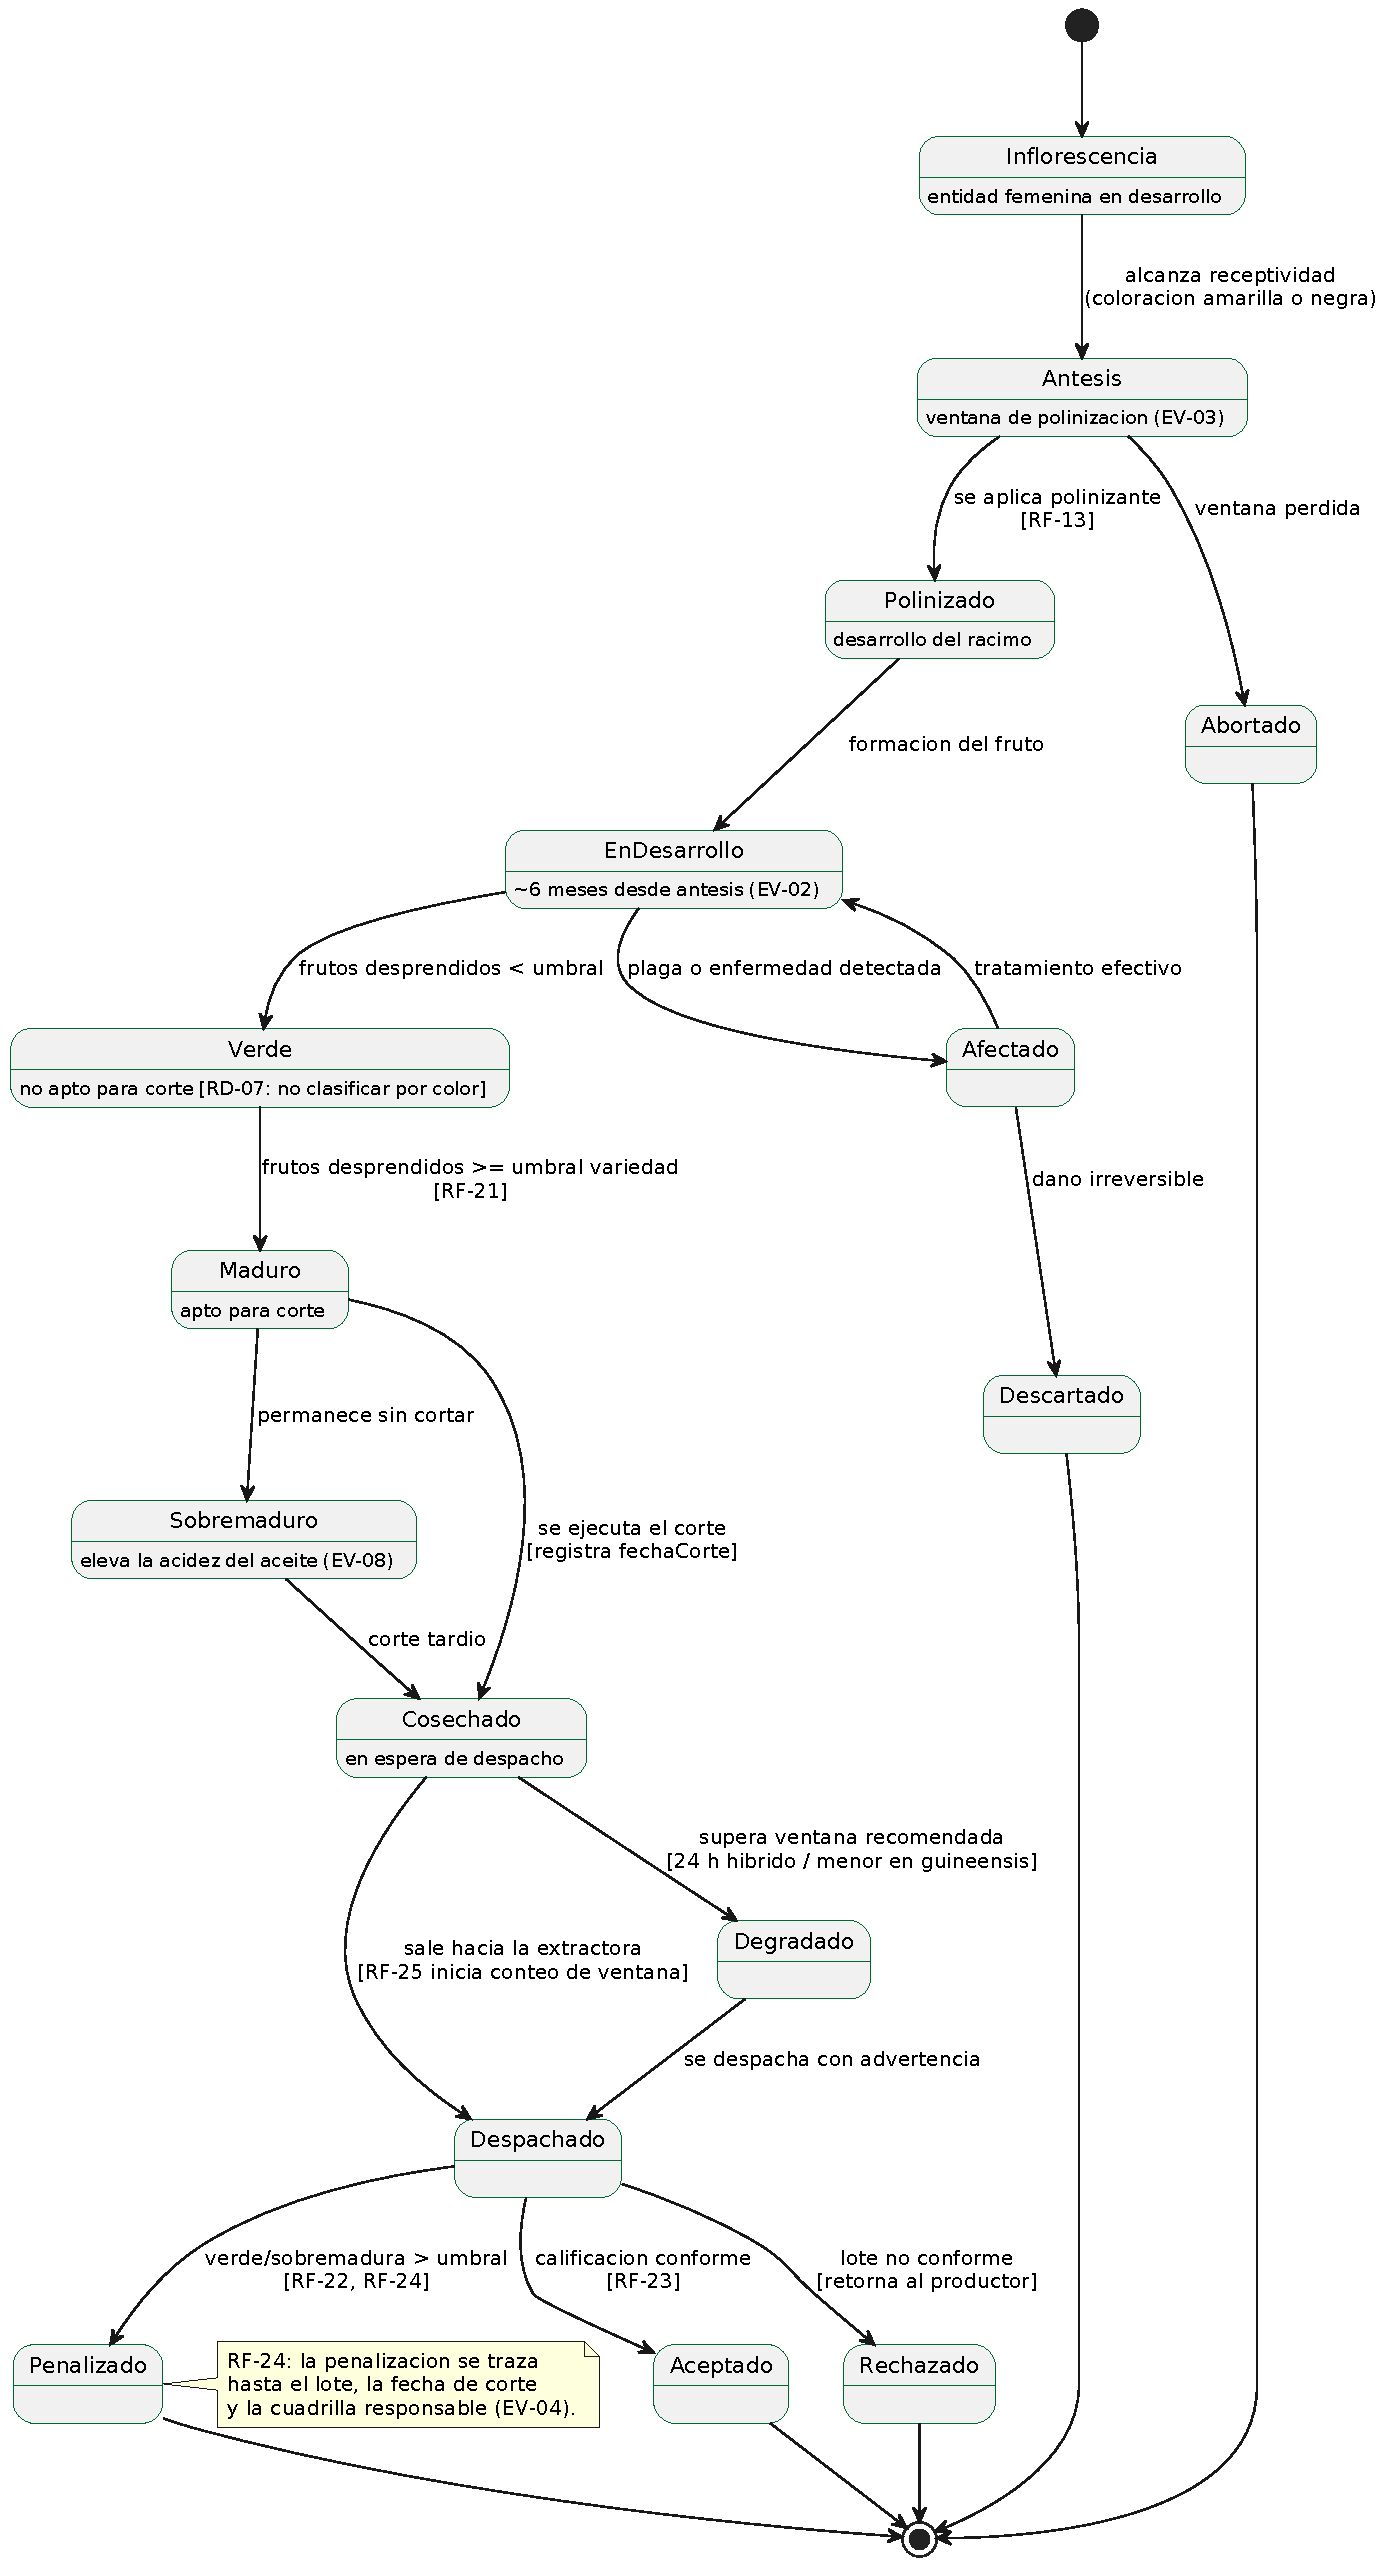
\includegraphics[width=0.67\textwidth]{img/estados_racimo}
\caption{Diagrama de estados del racimo, desde la inflorescencia hasta la calificación en la planta extractora.}
\label{fig:est_racimo}
\end{figure}

\begin{figure}[!htbp]
\centering
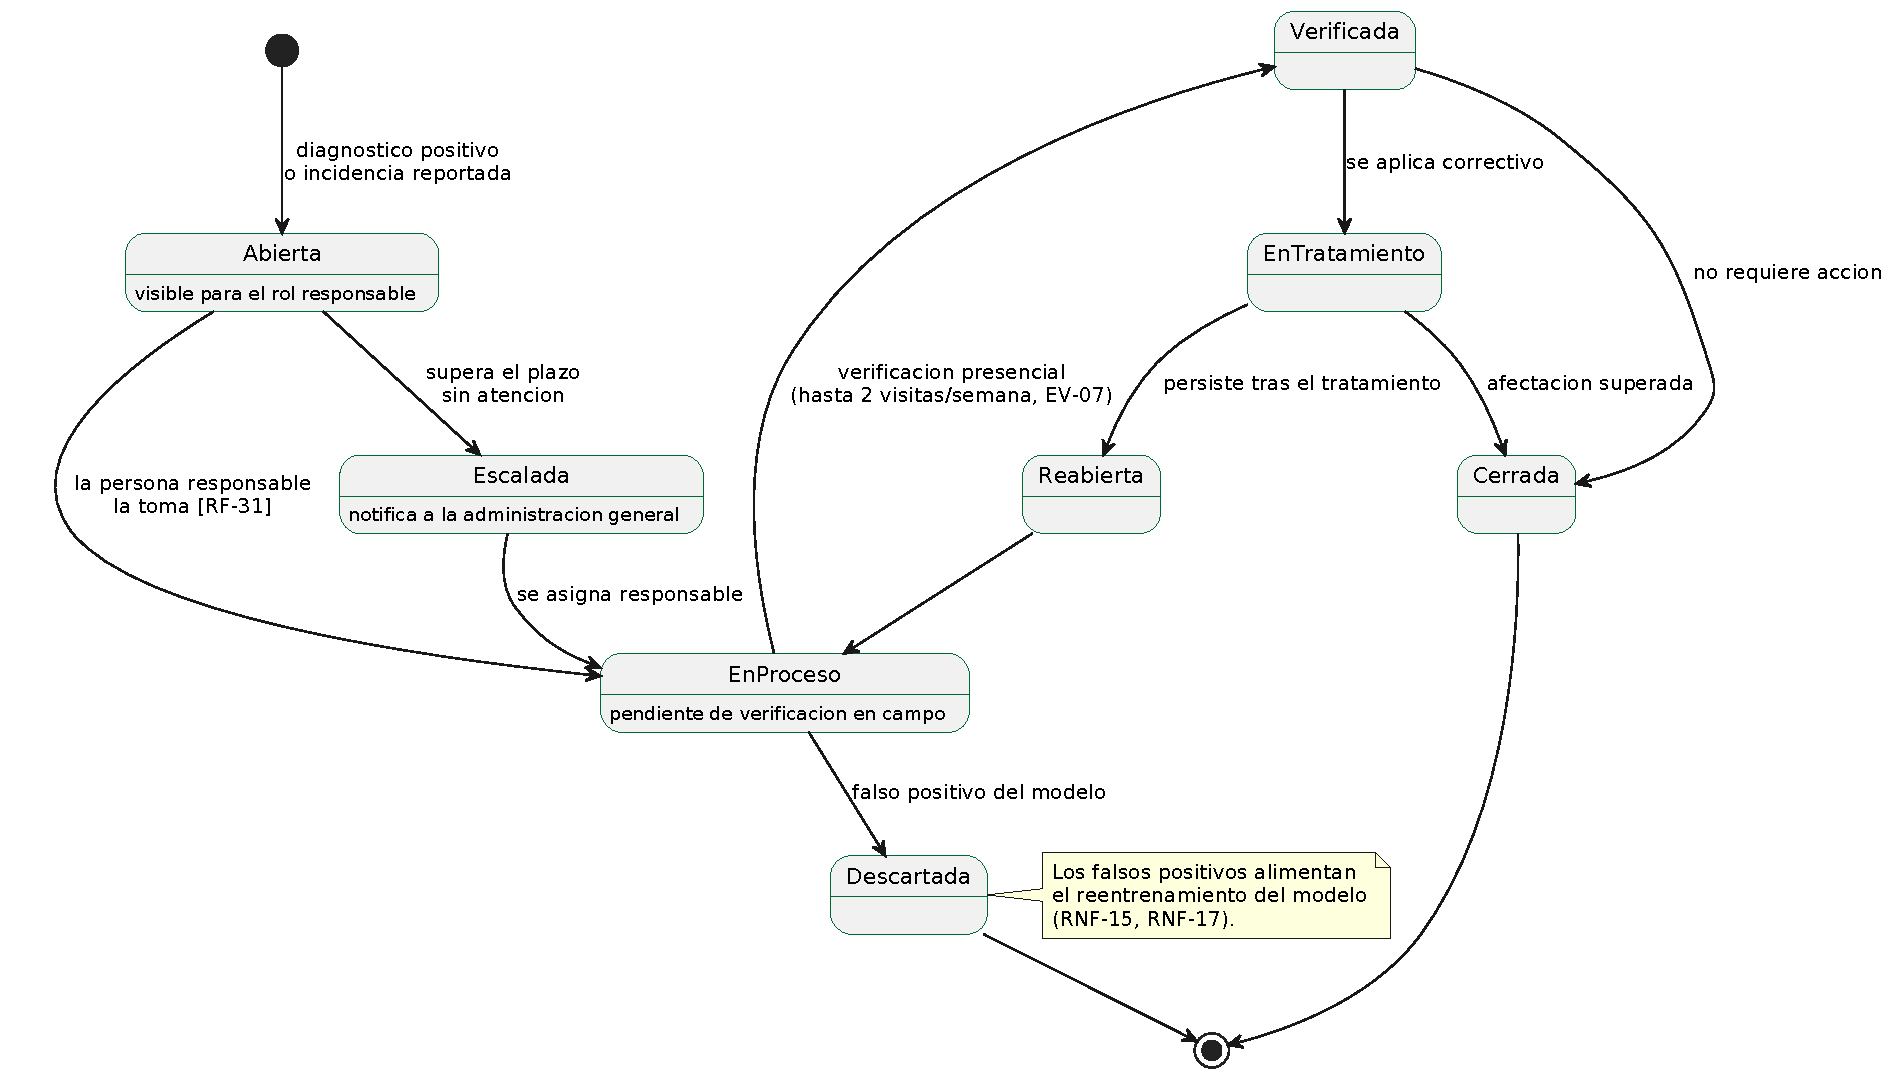
\includegraphics[width=1.0\textwidth]{img/estados_alerta}
\caption{Diagrama de estados de la alerta, con escalamiento por vencimiento de plazo y reapertura tras tratamiento inefectivo.}
\label{fig:est_alerta}
\end{figure}

\noindent
El estado \emph{Degradado} del racimo materializa el hallazgo de \id{EV-04} sobre la ventana entre
corte y entrega: el material híbrido tolera un intervalo mayor por su contenido de antioxidantes,
mientras que el \emph{guineensis} se deshidrata en dos o tres días. El estado \emph{Descartada} de
la alerta corresponde a los falsos positivos del modelo y alimenta el ciclo de reentrenamiento
previsto en \id{RNF-15} y \id{RNF-17}.

% ---------------------------------------------------------------------
\subsection{Diagrama de componentes}

\begin{figure}[!htbp]
\centering
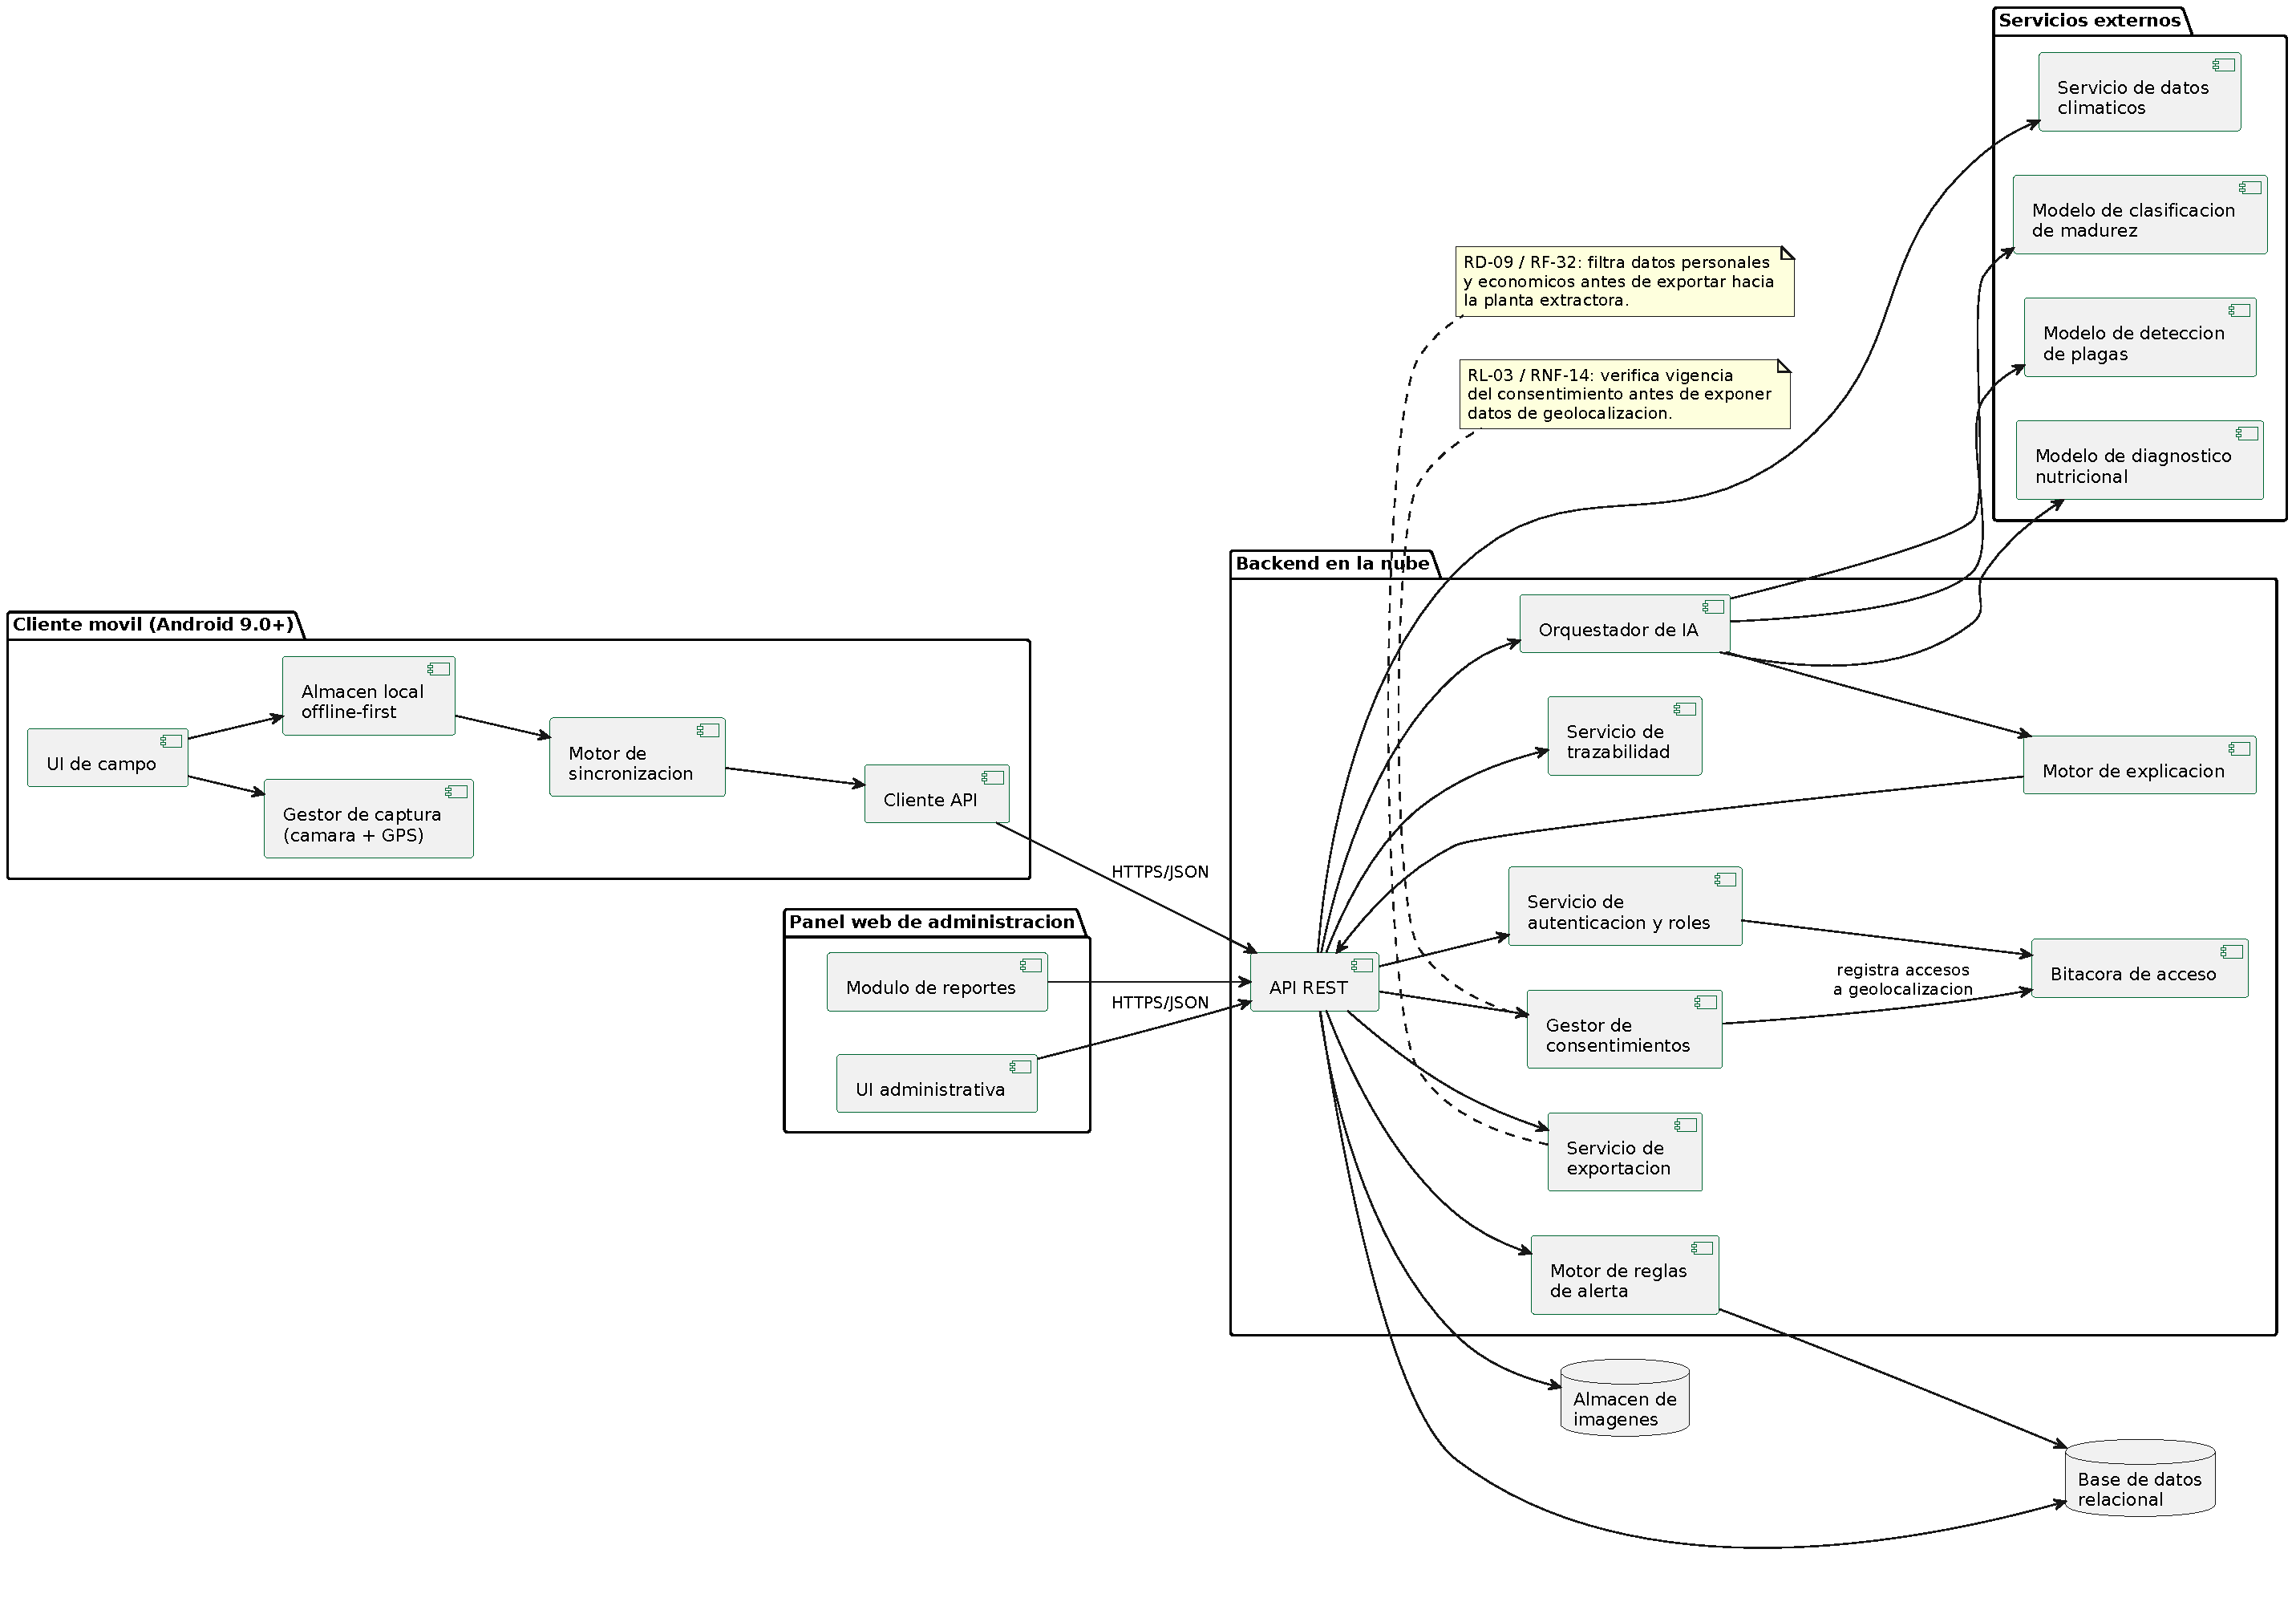
\includegraphics[width=1.0\textwidth]{img/componentes}
\caption{Diagrama de componentes del SIMPA.}
\label{fig:componentes}
\end{figure}

\noindent
Dos componentes merecen mención explícita por su origen normativo. El \emph{gestor de
consentimientos} verifica la vigencia antes de exponer cualquier dato de geolocalización y registra
todo acceso en la bitácora (\id{RL-03}, \id{RNF-14}). El \emph{servicio de exportación} filtra los
datos personales y económicos antes de generar el archivo destinado a la planta extractora
(\id{RD-09}, \id{RF-32}); su existencia como componente separado responde al criterio expreso de la
contraparte de que hay información que no puede compartirse (\id{EV-04}).

% ---------------------------------------------------------------------
\subsection{Diagrama de despliegue}

\begin{figure}[!htbp]
\centering
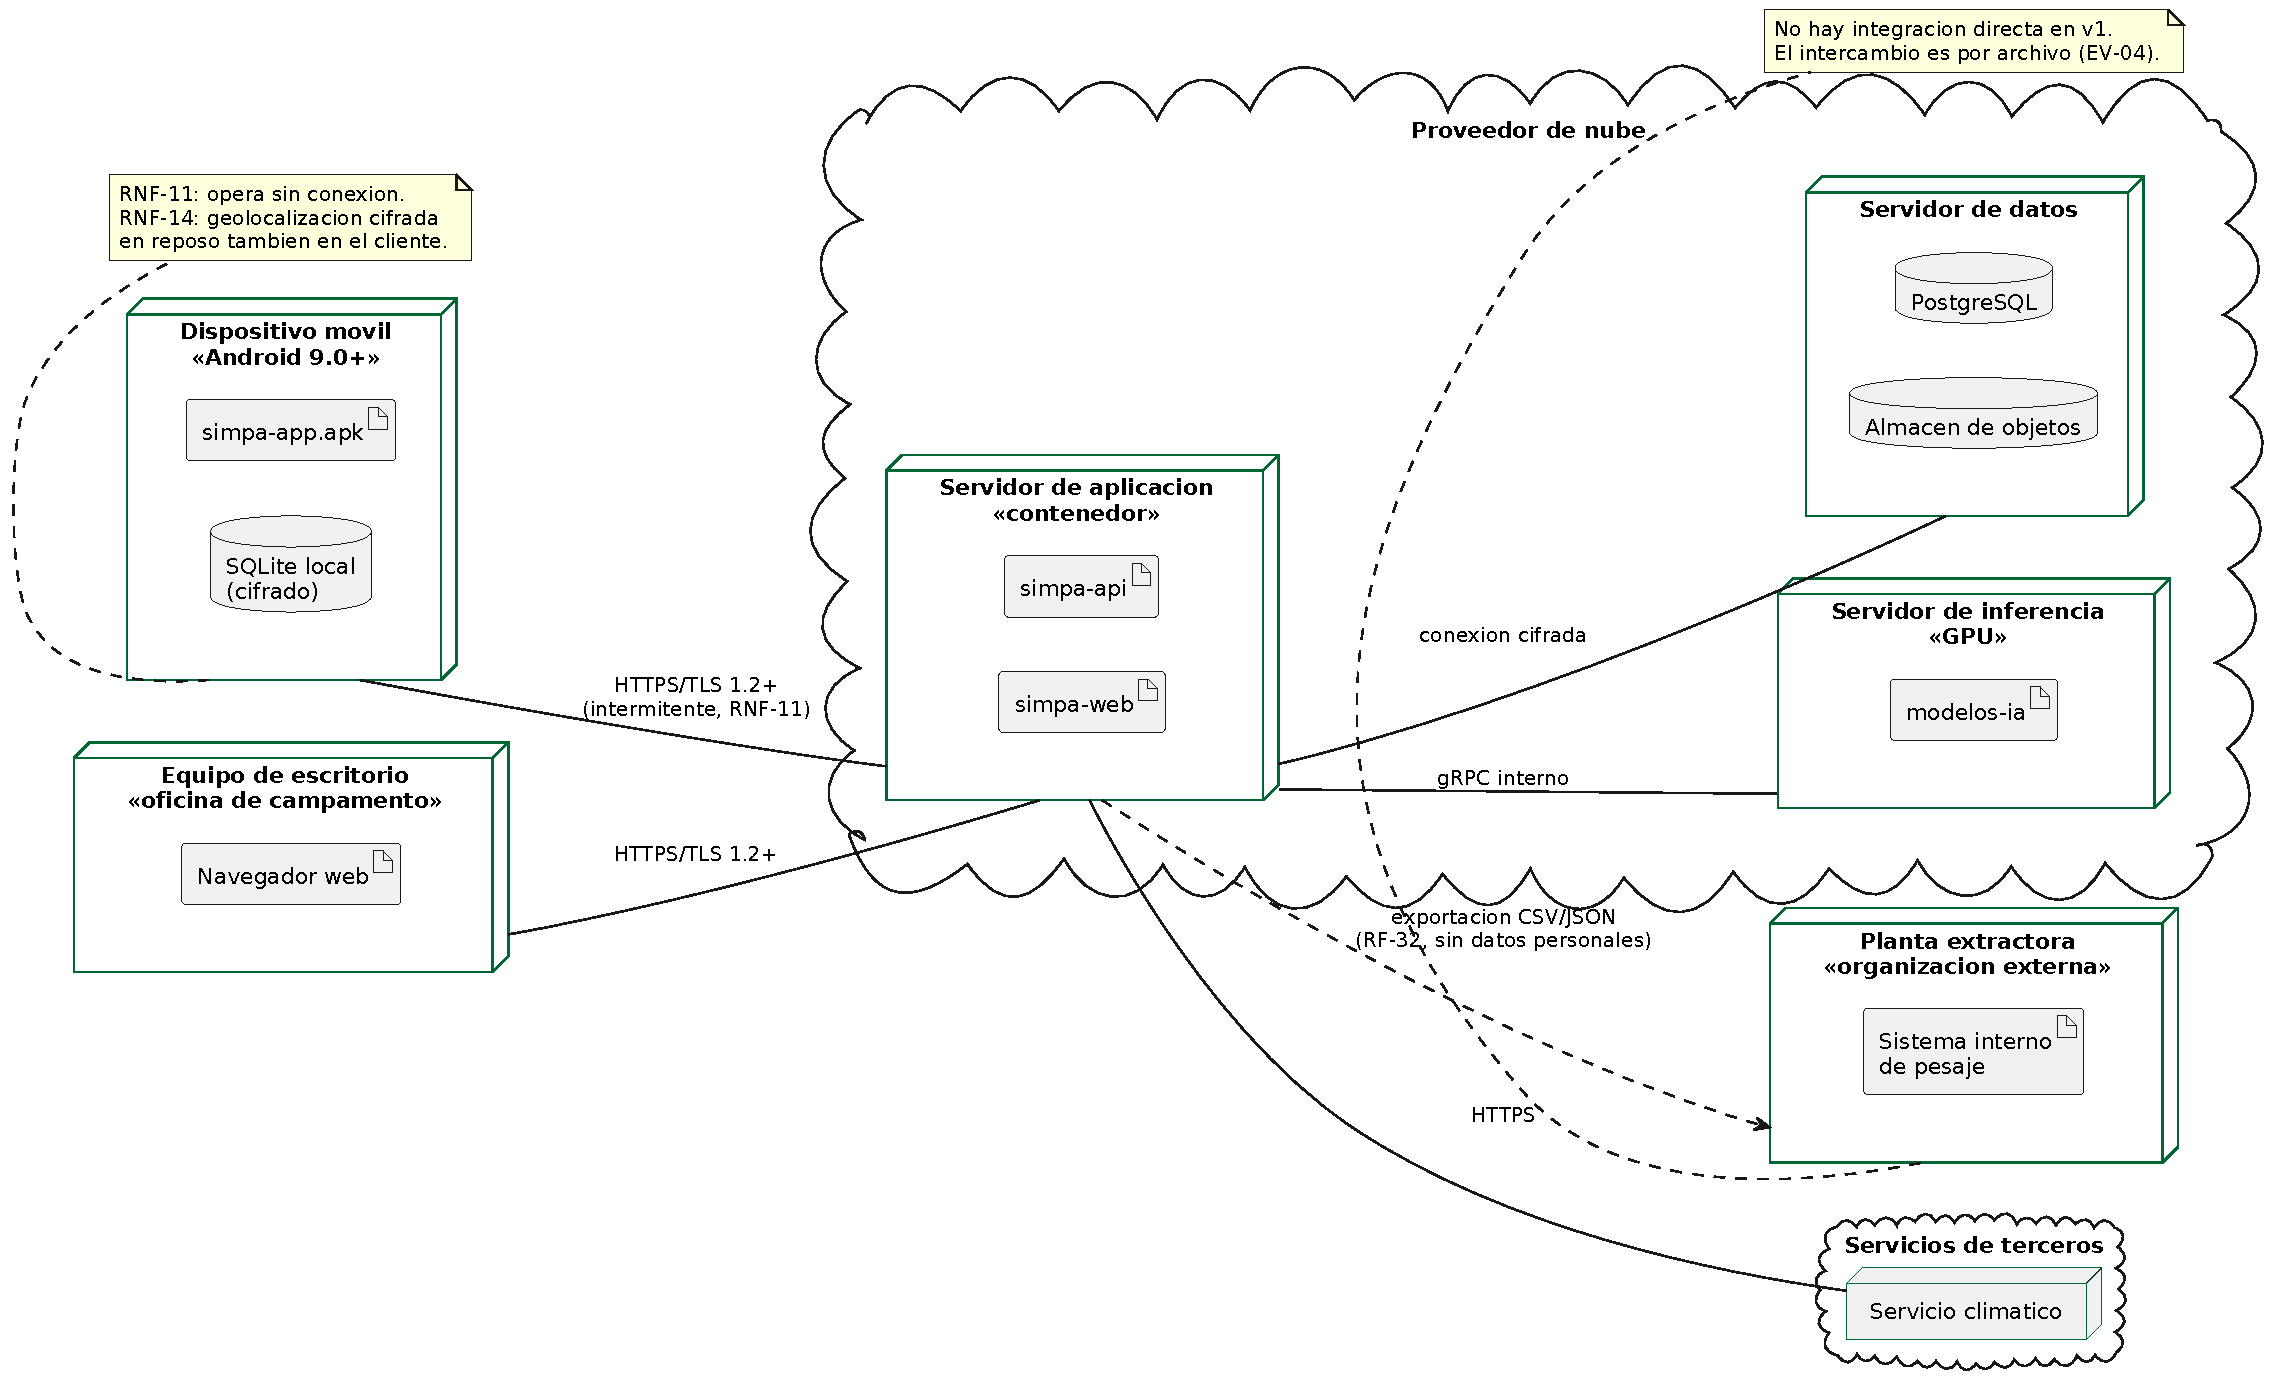
\includegraphics[width=1.0\textwidth]{img/despliegue}
\caption{Diagrama de despliegue del SIMPA.}
\label{fig:despliegue}
\end{figure}

\noindent
El enlace entre el dispositivo móvil y el servidor de aplicación se declara explícitamente como
\emph{intermitente}: el 74{,}2\% de las personas destinatarias no dispone de conectividad permanente
(\id{EV-12}). La planta extractora se representa como nodo externo sin integración directa; el
intercambio en la versión v1 se realiza por archivo, conforme a \id{RF-32}.

% ---------------------------------------------------------------------
\subsection{Cobertura del modelado}

\begin{longtable}{|L{4.6cm}|C{2.2cm}|C{2.2cm}|L{5.0cm}|}
\hline
\rowcolor{grisclaro}\textbf{Artefacto} & \textbf{Exigido} & \textbf{Entregado} & \textbf{Observación} \\
\hline
\endhead
Diagrama de casos de uso general & 1 & 1 & 8 actores, 18 casos de uso \\ \hline
Casos de uso detallados & 10 & 10 & Todos los \emph{Must}; $\geq 2$ flujos alternativos y $\geq 1$ excepción cada uno \\ \hline
Diagrama de clases refinado & 1 & 1 & 25 clases con atributos y operaciones \\ \hline
Diagramas de secuencia & CU \emph{Must} & 3 & CU-01, CU-03, CU-06 \\ \hline
Diagramas de actividad & Flujos principales & 1 & Ciclo semanal completo \\ \hline
Diagramas de estados & Entidades no triviales & 2 & Racimo y Alerta \\ \hline
Diagrama de componentes & 1 & 1 & --- \\ \hline
Diagrama de despliegue & 1 & 1 & --- \\ \hline
\caption{Cobertura del modelado UML frente a lo exigido en la §3.4 de la guía}
\end{longtable}

%  Requiere las imagenes en img/ generadas desde 03_Modelado/Diagramas_UML/
% =====================================================================

\newpage
\section{Modelado del sistema con UML}

El modelado emplea UML 2.5. Conforme a la §3.4 de la guía de la Entrega 3, se presentan ocho
diagramas: casos de uso general, especificación textual de diez casos de uso, clases refinado con
atributos y operaciones, tres diagramas de secuencia para los casos de uso \emph{Must}, actividad,
estados, componentes y despliegue. Todos se elaboraron en PlantUML y se entregan por triplicado
(fuente \id{.puml}, PNG a 300 dpi y SVG) en \id{03\_Modelado/Diagramas\_UML/}.

% ---------------------------------------------------------------------
\subsection{Diagrama general de casos de uso}

El diagrama presenta ocho actores y dieciocho casos de uso. Los actores primarios corresponden a los
seis perfiles de usuario de la §2.3; los actores secundarios son el servicio de análisis de IA y el
receptor GPS del dispositivo.

\begin{figure}[!htbp]
\centering
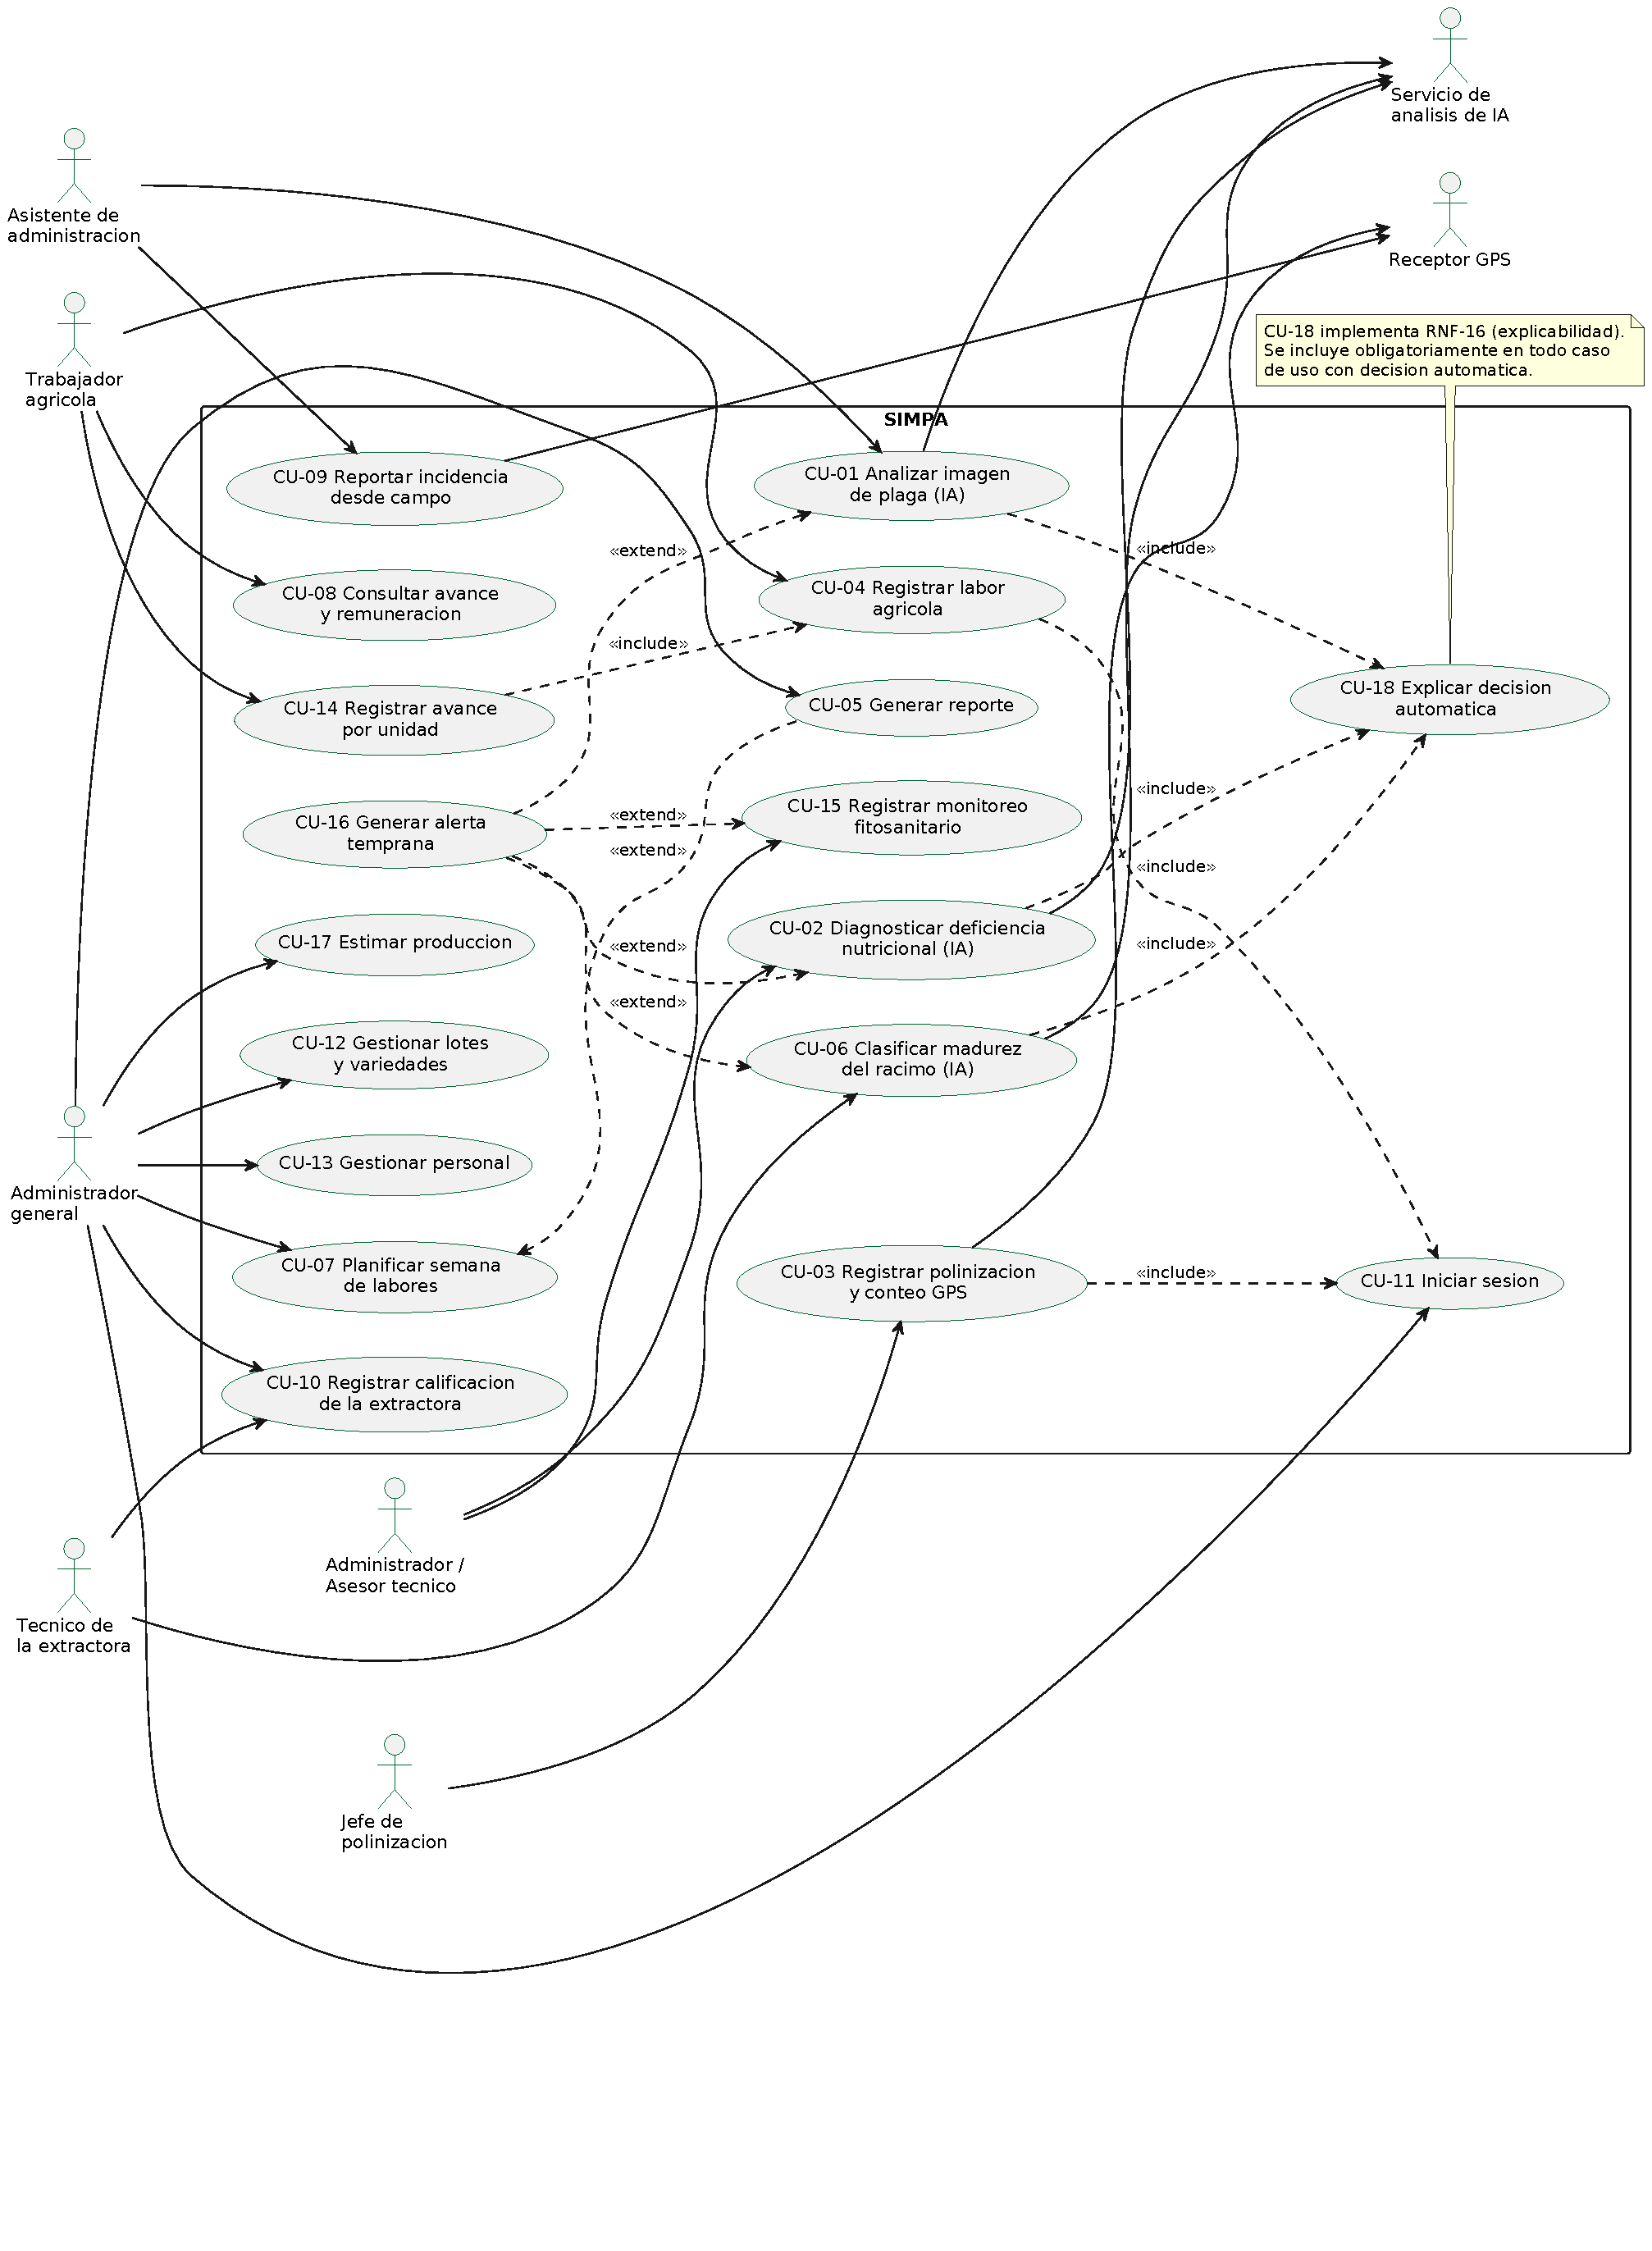
\includegraphics[width=0.91\textwidth]{img/casos_uso_general}
\caption{Diagrama general de casos de uso del SIMPA, con los ocho actores y el límite del sistema.}
\label{fig:cu_general}
\end{figure}

\noindent\textbf{Relaciones de inclusión y extensión.} \id{CU-14} incluye a \id{CU-04}, dado que el
registro de avance presupone una labor registrada. \id{CU-04} y \id{CU-03} incluyen a \id{CU-11},
por requerir sesión autenticada. Los tres casos de uso con decisión automática ---\id{CU-01},
\id{CU-02} y \id{CU-06}--- incluyen obligatoriamente a \id{CU-18}, que materializa el requisito de
explicabilidad \id{RNF-16}: no existe decisión automática sin explicación asociada. \id{CU-16}
extiende a los casos de diagnóstico y de monitoreo, puesto que la alerta se genera únicamente si el
resultado es positivo.

% ---------------------------------------------------------------------
\subsection{Especificación textual de los casos de uso}

Se especifican diez casos de uso, correspondientes a la totalidad de los requisitos funcionales de
prioridad \emph{Must}. Cada especificación incluye actores, precondiciones, postcondiciones, flujo
principal, al menos un flujo alternativo y al menos una excepción.

% --- CU-01
\begin{longtable}{|L{3.4cm}|L{12.0cm}|}
\hline
\rowcolor{grisclaro}\multicolumn{2}{|l|}{\textbf{CU-01 --- Analizar imagen para detectar plaga o enfermedad}}\\
\hline
\textbf{Requisitos} & \id{RF-07}, \id{RF-09}, \id{RF-12}, \id{RNF-16} \\ \hline
\textbf{Actores} & Primario: técnico fitosanitario / asistente de administración. Secundario: servicio de análisis de IA. \\ \hline
\textbf{Precondición} & Persona usuaria autenticada; lote seleccionado; cámara disponible. \\ \hline
\textbf{Postcondición} & El diagnóstico y su explicación quedan registrados y asociados al lote y a la fecha. \\ \hline
\textbf{Flujo principal} & 1. La persona usuaria selecciona el lote y la opción \emph{Analizar imagen}. \newline 2. Captura la fotografía de la palma o de la hoja. \newline 3. El sistema valida la calidad de la imagen. \newline 4. El sistema envía la imagen al servicio de IA con los parámetros de la variedad del lote. \newline 5. El servicio devuelve la clase de afectación, el nivel de confianza y el rasgo visual determinante. \newline 6. El sistema genera la explicación conforme a \id{RNF-16}. \newline 7. El sistema muestra el resultado, la explicación y la recomendación de control, y registra el diagnóstico. \\ \hline
\textbf{Flujo alternativo A} & \emph{Sin conectividad.} En el paso 4 el sistema almacena la imagen localmente y encola el análisis; al restablecerse la conexión lo ejecuta y notifica el resultado (\id{RNF-11}). \\ \hline
\textbf{Flujo alternativo B} & \emph{Confianza insuficiente.} Si el nivel de confianza es inferior al umbral configurado, el sistema no emite clasificación: informa que el resultado no es concluyente y sugiere repetir la captura o consultar a la asesoría técnica. \\ \hline
\textbf{Excepción E1} & Imagen de calidad insuficiente: el sistema solicita repetir la captura indicando el defecto detectado. \\ \hline
\textbf{Excepción E2} & Servicio de IA no disponible: el análisis queda en estado pendiente y la persona usuaria es notificada. \\ \hline
\textbf{Extensión} & Si el resultado es positivo, se ejecuta \id{CU-16} (generar alerta temprana). \\ \hline
\caption{CU-01 --- Analizar imagen para detectar plaga o enfermedad}
\end{longtable}

% --- CU-02
\begin{longtable}{|L{3.4cm}|L{12.0cm}|}
\hline
\rowcolor{grisclaro}\multicolumn{2}{|l|}{\textbf{CU-02 --- Diagnosticar deficiencia nutricional por imagen}}\\
\hline
\textbf{Requisitos} & \id{RF-08}, \id{RF-11}, \id{RNF-16} \\ \hline
\textbf{Actores} & Primario: administrador / asesor técnico. Secundario: servicio de análisis de IA. \\ \hline
\textbf{Precondición} & Persona usuaria autenticada; lote seleccionado con variedad asignada. \\ \hline
\textbf{Postcondición} & El diagnóstico nutricional y su recomendación quedan registrados en el historial del lote. \\ \hline
\textbf{Flujo principal} & 1. La persona usuaria selecciona \emph{Diagnóstico nutricional} y el lote. \newline 2. Captura la fotografía de la hoja. \newline 3. El sistema valida la imagen y la envía al servicio de IA. \newline 4. El servicio estima el elemento deficiente. \newline 5. El sistema genera una explicación de tipo causal, indicando qué signo foliar sustenta la estimación. \newline 6. El sistema muestra la deficiencia, la recomendación de fertilización y la explicación, y registra el diagnóstico. \\ \hline
\textbf{Flujo alternativo A} & La persona usuaria adjunta una imagen existente de la galería en lugar de capturarla. \\ \hline
\textbf{Flujo alternativo B} & \emph{Contraste con análisis de laboratorio.} Si el lote tiene un análisis de suelo o foliar registrado (\id{RF-11}), el sistema contrasta la estimación con los valores medidos y señala la discrepancia si la hubiere. \\ \hline
\textbf{Excepción E1} & Imagen no válida: el sistema solicita repetir la captura. \\ \hline
\textbf{Excepción E2} & Lote sin variedad asignada: el sistema advierte que la estimación puede no ser aplicable y solicita completar el dato. \\ \hline
\textbf{Extensión} & Si la deficiencia estimada es severa, se ejecuta \id{CU-16}. \\ \hline
\caption{CU-02 --- Diagnosticar deficiencia nutricional por imagen}
\end{longtable}

% --- CU-03
\begin{longtable}{|L{3.4cm}|L{12.0cm}|}
\hline
\rowcolor{grisclaro}\multicolumn{2}{|l|}{\textbf{CU-03 --- Registrar polinización y conteo georreferenciado}}\\
\hline
\textbf{Requisitos} & \id{RF-13}, \id{RF-14}, \id{RNF-05}, \id{RNF-12}, \id{RL-03} \\ \hline
\textbf{Actores} & Primario: polinizador. Secundario: receptor GPS. \\ \hline
\textbf{Precondición} & Lote en etapa de polinización; sesión iniciada; consentimiento de geolocalización vigente. \\ \hline
\textbf{Postcondición} & La polinización y el conteo diario quedan registrados por persona, lote y fecha, sin ingreso manual planta por planta. \\ \hline
\textbf{Flujo principal} & 1. El polinizador inicia la jornada en el lote. \newline 2. El sistema verifica la vigencia del consentimiento de geolocalización. \newline 3. El sistema activa el rastreo con período de muestreo de 30 s. \newline 4. Durante la jornada, el sistema almacena las marcaciones georreferenciadas. \newline 5. El polinizador registra el estado de la antesis y la verificación visual. \newline 6. Al cierre, el sistema calcula el número de flores polinizadas a partir de las marcaciones. \newline 7. El sistema almacena el registro y muestra el total a la persona trabajadora. \\ \hline
\textbf{Flujo alternativo A} & \emph{Consentimiento revocado.} Si el consentimiento no está vigente, el sistema no activa el rastreo y habilita el registro manual del número de flores, sin penalización para la persona trabajadora (\id{RL-03}). \\ \hline
\textbf{Flujo alternativo B} & \emph{Sin conectividad.} Las marcaciones se almacenan localmente y se sincronizan al reconectar (\id{RNF-11}). \\ \hline
\textbf{Excepción E1} & Precisión GPS superior a 10 m: el sistema conserva el dato marcándolo como de precisión degradada y advierte a la persona usuaria, sin descartar la jornada (\id{RNF-12}). \\ \hline
\textbf{Excepción E2} & Pérdida total de señal GPS durante la jornada: el sistema conserva el tramo registrado y solicita completar el conteo de forma manual para el tramo faltante. \\ \hline
\caption{CU-03 --- Registrar polinización y conteo georreferenciado}
\end{longtable}

% --- CU-04
\begin{longtable}{|L{3.4cm}|L{12.0cm}|}
\hline
\rowcolor{grisclaro}\multicolumn{2}{|l|}{\textbf{CU-04 --- Registrar labor agrícola}}\\
\hline
\textbf{Requisitos} & \id{RF-04}, \id{RF-28}, \id{RF-35} \\ \hline
\textbf{Actores} & Primario: trabajador agrícola. Alternativo: jefe de campo (registro delegado). \\ \hline
\textbf{Precondición} & Lote y persona trabajadora registrados; persona usuaria autenticada. \\ \hline
\textbf{Postcondición} & La labor y su avance quedan en el historial del lote y computan para el cumplimiento del plan semanal. \\ \hline
\textbf{Flujo principal} & 1. La persona usuaria selecciona el lote y el tipo de labor. \newline 2. Ingresa la cantidad ejecutada en la unidad correspondiente. \newline 3. El sistema valida que la unidad corresponda al tipo de labor. \newline 4. El sistema registra la labor asociada al lote, la fecha y la persona responsable. \newline 5. El sistema actualiza el avance acumulado del período y el cumplimiento de la meta semanal. \\ \hline
\textbf{Flujo alternativo A} & \emph{Registro delegado.} Si la persona trabajadora no dispone de dispositivo propio, el jefe de campo registra el avance en su nombre; el sistema conserva en bitácora la identidad de quien efectuó el registro (\id{RF-35}, \id{RD-10}). \\ \hline
\textbf{Flujo alternativo B} & \emph{Sin conectividad.} La labor se almacena localmente y se sincroniza al reconectar. \\ \hline
\textbf{Excepción E1} & Datos incompletos: el sistema impide guardar y señala los campos faltantes. \\ \hline
\textbf{Excepción E2} & Unidad incompatible con el tipo de labor: el sistema rechaza el registro e indica la unidad esperada. \\ \hline
\caption{CU-04 --- Registrar labor agrícola}
\end{longtable}

% --- CU-05
\begin{longtable}{|L{3.4cm}|L{12.0cm}|}
\hline
\rowcolor{grisclaro}\multicolumn{2}{|l|}{\textbf{CU-05 --- Generar reporte}}\\
\hline
\textbf{Requisitos} & \id{RF-19}, \id{RF-26} \\ \hline
\textbf{Actores} & Primario: administrador general. \\ \hline
\textbf{Precondición} & Existen registros en el período seleccionado. \\ \hline
\textbf{Postcondición} & El reporte queda disponible para consulta o exportación. \\ \hline
\textbf{Flujo principal} & 1. La persona administradora selecciona el tipo de reporte y el período. \newline 2. El sistema consolida labores, avance, producción y alertas del período. \newline 3. El sistema genera y presenta el reporte. \newline 4. La persona administradora lo consulta o lo exporta a PDF o a hoja de cálculo. \\ \hline
\textbf{Flujo alternativo A} & Filtrado por lote, por equipo o por persona trabajadora. \\ \hline
\textbf{Flujo alternativo B} & \emph{Reporte de cumplimiento semanal.} El sistema contrasta el plan de la semana con lo ejecutado y destaca las metas no alcanzadas y su remanente. \\ \hline
\textbf{Excepción E1} & Sin registros en el período: el sistema informa la ausencia de datos y propone un período alternativo con información disponible. \\ \hline
\caption{CU-05 --- Generar reporte}
\end{longtable}

% --- CU-06
\begin{longtable}{|L{3.4cm}|L{12.0cm}|}
\hline
\rowcolor{grisclaro}\multicolumn{2}{|l|}{\textbf{CU-06 --- Clasificar la madurez del racimo}}\\
\hline
\textbf{Requisitos} & \id{RF-21}, \id{RF-22}, \id{RD-07}, \id{RD-08}, \id{RNF-01}, \id{RNF-16} \\ \hline
\textbf{Actores} & Primario: cosechador / técnico de la extractora. Secundario: servicio de análisis de IA. \\ \hline
\textbf{Precondición} & Lote con variedad asignada; persona usuaria autenticada. \\ \hline
\textbf{Postcondición} & La clasificación queda asociada al racimo, al lote y a la fecha, y actualiza el porcentaje estimado de fruta verde del lote. \\ \hline
\textbf{Flujo principal} & 1. La persona usuaria selecciona el lote y la opción \emph{Clasificar racimo}. \newline 2. El sistema recupera el umbral de desprendimiento de la variedad del lote. \newline 3. La persona usuaria captura la fotografía de la parte basal del racimo. \newline 4. El servicio de IA cuenta los frutos desprendidos, sin emplear el color como criterio (\id{RD-07}). \newline 5. El sistema compara el conteo con el umbral de la variedad y determina el estado. \newline 6. El sistema genera una explicación por contraste, indicando el conteo obtenido y el umbral aplicable. \newline 7. El sistema registra la clasificación y actualiza el porcentaje de fruta verde del lote. \\ \hline
\textbf{Flujo alternativo A} & \emph{Verificación previa al despacho.} La persona usuaria solicita el porcentaje estimado de fruta verde del lote; si alcanza o supera el umbral de penalización, el sistema emite alerta preventiva y desaconseja el despacho (\id{RF-22}). \\ \hline
\textbf{Flujo alternativo B} & \emph{Sobremadurez.} Si el conteo excede ampliamente el umbral, el sistema clasifica el racimo como sobremaduro y advierte sobre el incremento de acidez. \\ \hline
\textbf{Excepción E1} & Lote sin variedad asignada: el sistema no clasifica y solicita completar el dato, dado que el umbral depende de la variedad. \\ \hline
\textbf{Excepción E2} & Parte basal no visible en la imagen: el sistema solicita repetir la captura indicando el encuadre requerido. \\ \hline
\caption{CU-06 --- Clasificar la madurez del racimo}
\end{longtable}

% --- CU-07
\begin{longtable}{|L{3.4cm}|L{12.0cm}|}
\hline
\rowcolor{grisclaro}\multicolumn{2}{|l|}{\textbf{CU-07 --- Planificar la semana de labores}}\\
\hline
\textbf{Requisitos} & \id{RF-26}, \id{RF-27}, \id{RF-34}, \id{RF-37} a \id{RF-39} \\ \hline
\textbf{Actores} & Primario: administrador general. \\ \hline
\textbf{Precondición} & Lotes y tipos de labor registrados. \\ \hline
\textbf{Postcondición} & El plan de la semana queda publicado y disponible para el seguimiento diario. \\ \hline
\textbf{Flujo principal} & 1. La persona administradora crea el plan de la semana. \newline 2. Para cada lote, define las labores previstas con su meta y unidad. \newline 3. El sistema incorpora automáticamente los remanentes arrastrados de la semana anterior. \newline 4. La persona administradora registra los insumos requeridos. \newline 5. El sistema publica el plan y lo hace visible al jefe de campo. \\ \hline
\textbf{Flujo alternativo A} & \emph{Cierre de semana.} Al cierre, el sistema calcula el cumplimiento de cada meta; si es parcial, genera el remanente como labor pendiente de la semana siguiente, vinculada a la de origen (\id{RF-27}). \\ \hline
\textbf{Flujo alternativo B} & Ajuste del plan durante la semana en curso, conservando la versión previa en bitácora. \\ \hline
\textbf{Flujo alternativo C} & \emph{Liquidación y aprobación.} Al cierre, el sistema genera la liquidación que contrasta cantidad presupuestada, cantidad ejecutada, tarifa y valor por grupo de labor, totaliza el gasto presupuestado frente al real, e incorpora las labores no presupuestadas en su grupo diferenciado (\id{RF-37}, \id{RF-38}). La persona administradora aprueba la liquidación y el período queda cerrado (\id{RF-39}). \\ \hline
\textbf{Excepción E1} & Meta expresada en unidad incompatible con el tipo de labor: el sistema rechaza la meta e indica la unidad esperada. \\ \hline
\textbf{Excepción E2} & Existe un plan publicado para la misma semana: el sistema advierte y solicita confirmación antes de sustituirlo. \\ \hline
\caption{CU-07 --- Planificar la semana de labores}
\end{longtable}

% --- CU-08
\begin{longtable}{|L{3.4cm}|L{12.0cm}|}
\hline
\rowcolor{grisclaro}\multicolumn{2}{|l|}{\textbf{CU-08 --- Consultar avance acumulado y remuneración estimada}}\\
\hline
\textbf{Requisitos} & \id{RF-29}, \id{RF-36}, \id{RL-04} \\ \hline
\textbf{Actores} & Primario: trabajador agrícola. \\ \hline
\textbf{Precondición} & Existen registros de avance de la persona trabajadora en el período. \\ \hline
\textbf{Postcondición} & Se presenta el consolidado del período, sin posibilidad de edición por parte de la persona trabajadora. \\ \hline
\textbf{Flujo principal} & 1. La persona trabajadora accede a \emph{Mi avance}. \newline 2. Selecciona el período (quincena en curso por defecto). \newline 3. El sistema agrega sus registros de avance por tipo de labor. \newline 4. El sistema obtiene del catálogo la tarifa vigente de cada tipo de labor a la fecha de cada registro y calcula la remuneración estimada correspondiente al trabajo por avance. \newline 5. El sistema presenta el desglose por labor y el total estimado. \\ \hline
\textbf{Flujo alternativo A} & \emph{Ejercicio del derecho de acceso.} La persona trabajadora solicita la exportación de sus datos personales; el sistema genera el archivo conforme al Art. 12 de la LOPDP (\id{RL-04}). \\ \hline
\textbf{Flujo alternativo B} & \emph{Discrepancia.} La persona trabajadora marca un registro como discrepante; el sistema notifica a la administración sin modificar el dato original, y la corrección se tramita mediante \id{RL-05}. \\ \hline
\textbf{Excepción E1} & Sin registros en el período: el sistema informa la ausencia de datos. \\ \hline
\textbf{Excepción E2} & La labor carece de tarifa vigente en el catálogo (\id{RF-36}) a la fecha del registro: el sistema muestra el avance en unidades, omite la estimación monetaria e indica que la tarifa no está vigente para esa fecha. \\ \hline
\caption{CU-08 --- Consultar avance acumulado y remuneración estimada}
\end{longtable}

% --- CU-09
\begin{longtable}{|L{3.4cm}|L{12.0cm}|}
\hline
\rowcolor{grisclaro}\multicolumn{2}{|l|}{\textbf{CU-09 --- Reportar incidencia desde el campo}}\\
\hline
\textbf{Requisitos} & \id{RF-30}, \id{RF-31}, \id{RF-12} \\ \hline
\textbf{Actores} & Primario: asistente de administración / trabajador agrícola. Secundario: receptor GPS. \\ \hline
\textbf{Precondición} & Persona usuaria autenticada; cámara y GPS disponibles. \\ \hline
\textbf{Postcondición} & La incidencia queda registrada con fotografía y coordenadas, e incorporada a la lista de pendientes de verificación. \\ \hline
\textbf{Flujo principal} & 1. La persona usuaria selecciona \emph{Reportar incidencia}. \newline 2. Captura la fotografía de la afectación. \newline 3. El sistema obtiene las coordenadas del punto. \newline 4. La persona usuaria selecciona el lote y describe la afectación. \newline 5. El sistema registra la incidencia georreferenciada. \newline 6. El sistema la incorpora a la lista de pendientes de la persona supervisora. \\ \hline
\textbf{Flujo alternativo A} & \emph{Análisis asistido.} La persona usuaria solicita el análisis de la fotografía; se ejecuta \id{CU-01} y el diagnóstico se asocia a la incidencia. \\ \hline
\textbf{Flujo alternativo B} & \emph{Verificación en visita.} La persona supervisora recorre su lista de pendientes, ubica la incidencia por sus coordenadas y la marca como verificada o descartada. \\ \hline
\textbf{Excepción E1} & GPS no disponible: el sistema registra la incidencia solicitando la selección manual del lote y la marca como de ubicación aproximada. \\ \hline
\textbf{Excepción E2} & Sin conectividad: la incidencia se encola y se sincroniza al reconectar, conservando el instante original de captura. \\ \hline
\caption{CU-09 --- Reportar incidencia desde el campo}
\end{longtable}

% --- CU-10
\begin{longtable}{|L{3.4cm}|L{12.0cm}|}
\hline
\rowcolor{grisclaro}\multicolumn{2}{|l|}{\textbf{CU-10 --- Registrar la calificación de la planta extractora}}\\
\hline
\textbf{Requisitos} & \id{RF-23}, \id{RF-24}, \id{RF-25}, \id{RF-33} \\ \hline
\textbf{Actores} & Primario: administrador general. \\ \hline
\textbf{Precondición} & Existe un despacho registrado con su fecha de corte. \\ \hline
\textbf{Postcondición} & La calificación queda asociada al lote de origen y disponible para el análisis de trazabilidad. \\ \hline
\textbf{Flujo principal} & 1. La persona administradora selecciona el despacho. \newline 2. Ingresa los datos del ticket de pesaje: peso bruto, tara y neto. \newline 3. Ingresa la calificación de calidad: tamaño del fruto, porcentaje de fruta verde, sobremadura, malformación y pedúnculo largo. \newline 4. El sistema calcula el intervalo entre el corte y la entrega. \newline 5. El sistema registra la calificación y la asocia al lote de origen. \\ \hline
\textbf{Flujo alternativo A} & \emph{Análisis de trazabilidad.} Ante una calificación desfavorable, la persona administradora consulta la cadena lote $\rightarrow$ fecha de corte $\rightarrow$ cuadrilla, y contrasta con las labores del período para distinguir si el origen está en la cosecha o en el manejo del cultivo (\id{RF-24}). \\ \hline
\textbf{Flujo alternativo B} & \emph{Ausencia de guía de remisión.} Si el despacho se registra sin número de guía, el sistema advierte antes del cierre (\id{RF-33}). \\ \hline
\textbf{Excepción E1} & El intervalo entre corte y entrega supera el valor recomendado para la variedad: el sistema registra la advertencia junto al despacho (\id{RF-25}). \\ \hline
\textbf{Excepción E2} & La suma de pesos es inconsistente (neto distinto de bruto menos tara): el sistema rechaza el registro e indica la inconsistencia. \\ \hline
\caption{CU-10 --- Registrar la calificación de la planta extractora}
\end{longtable}

% ---------------------------------------------------------------------
\subsection{Diagrama de clases refinado}

El modelo del dominio comprende veinticinco clases con atributos y operaciones. Incorpora tres
jerarquías de herencia (\id{Persona}--\id{Usuario} y la especialización de \id{Diagnostico} en sus
tres variantes), cuatro relaciones de composición y asociaciones con multiplicidad explícita. No
corresponde a un diseño de base de datos, sino al modelo conceptual del dominio del problema.

\begin{figure}[!htbp]
\centering
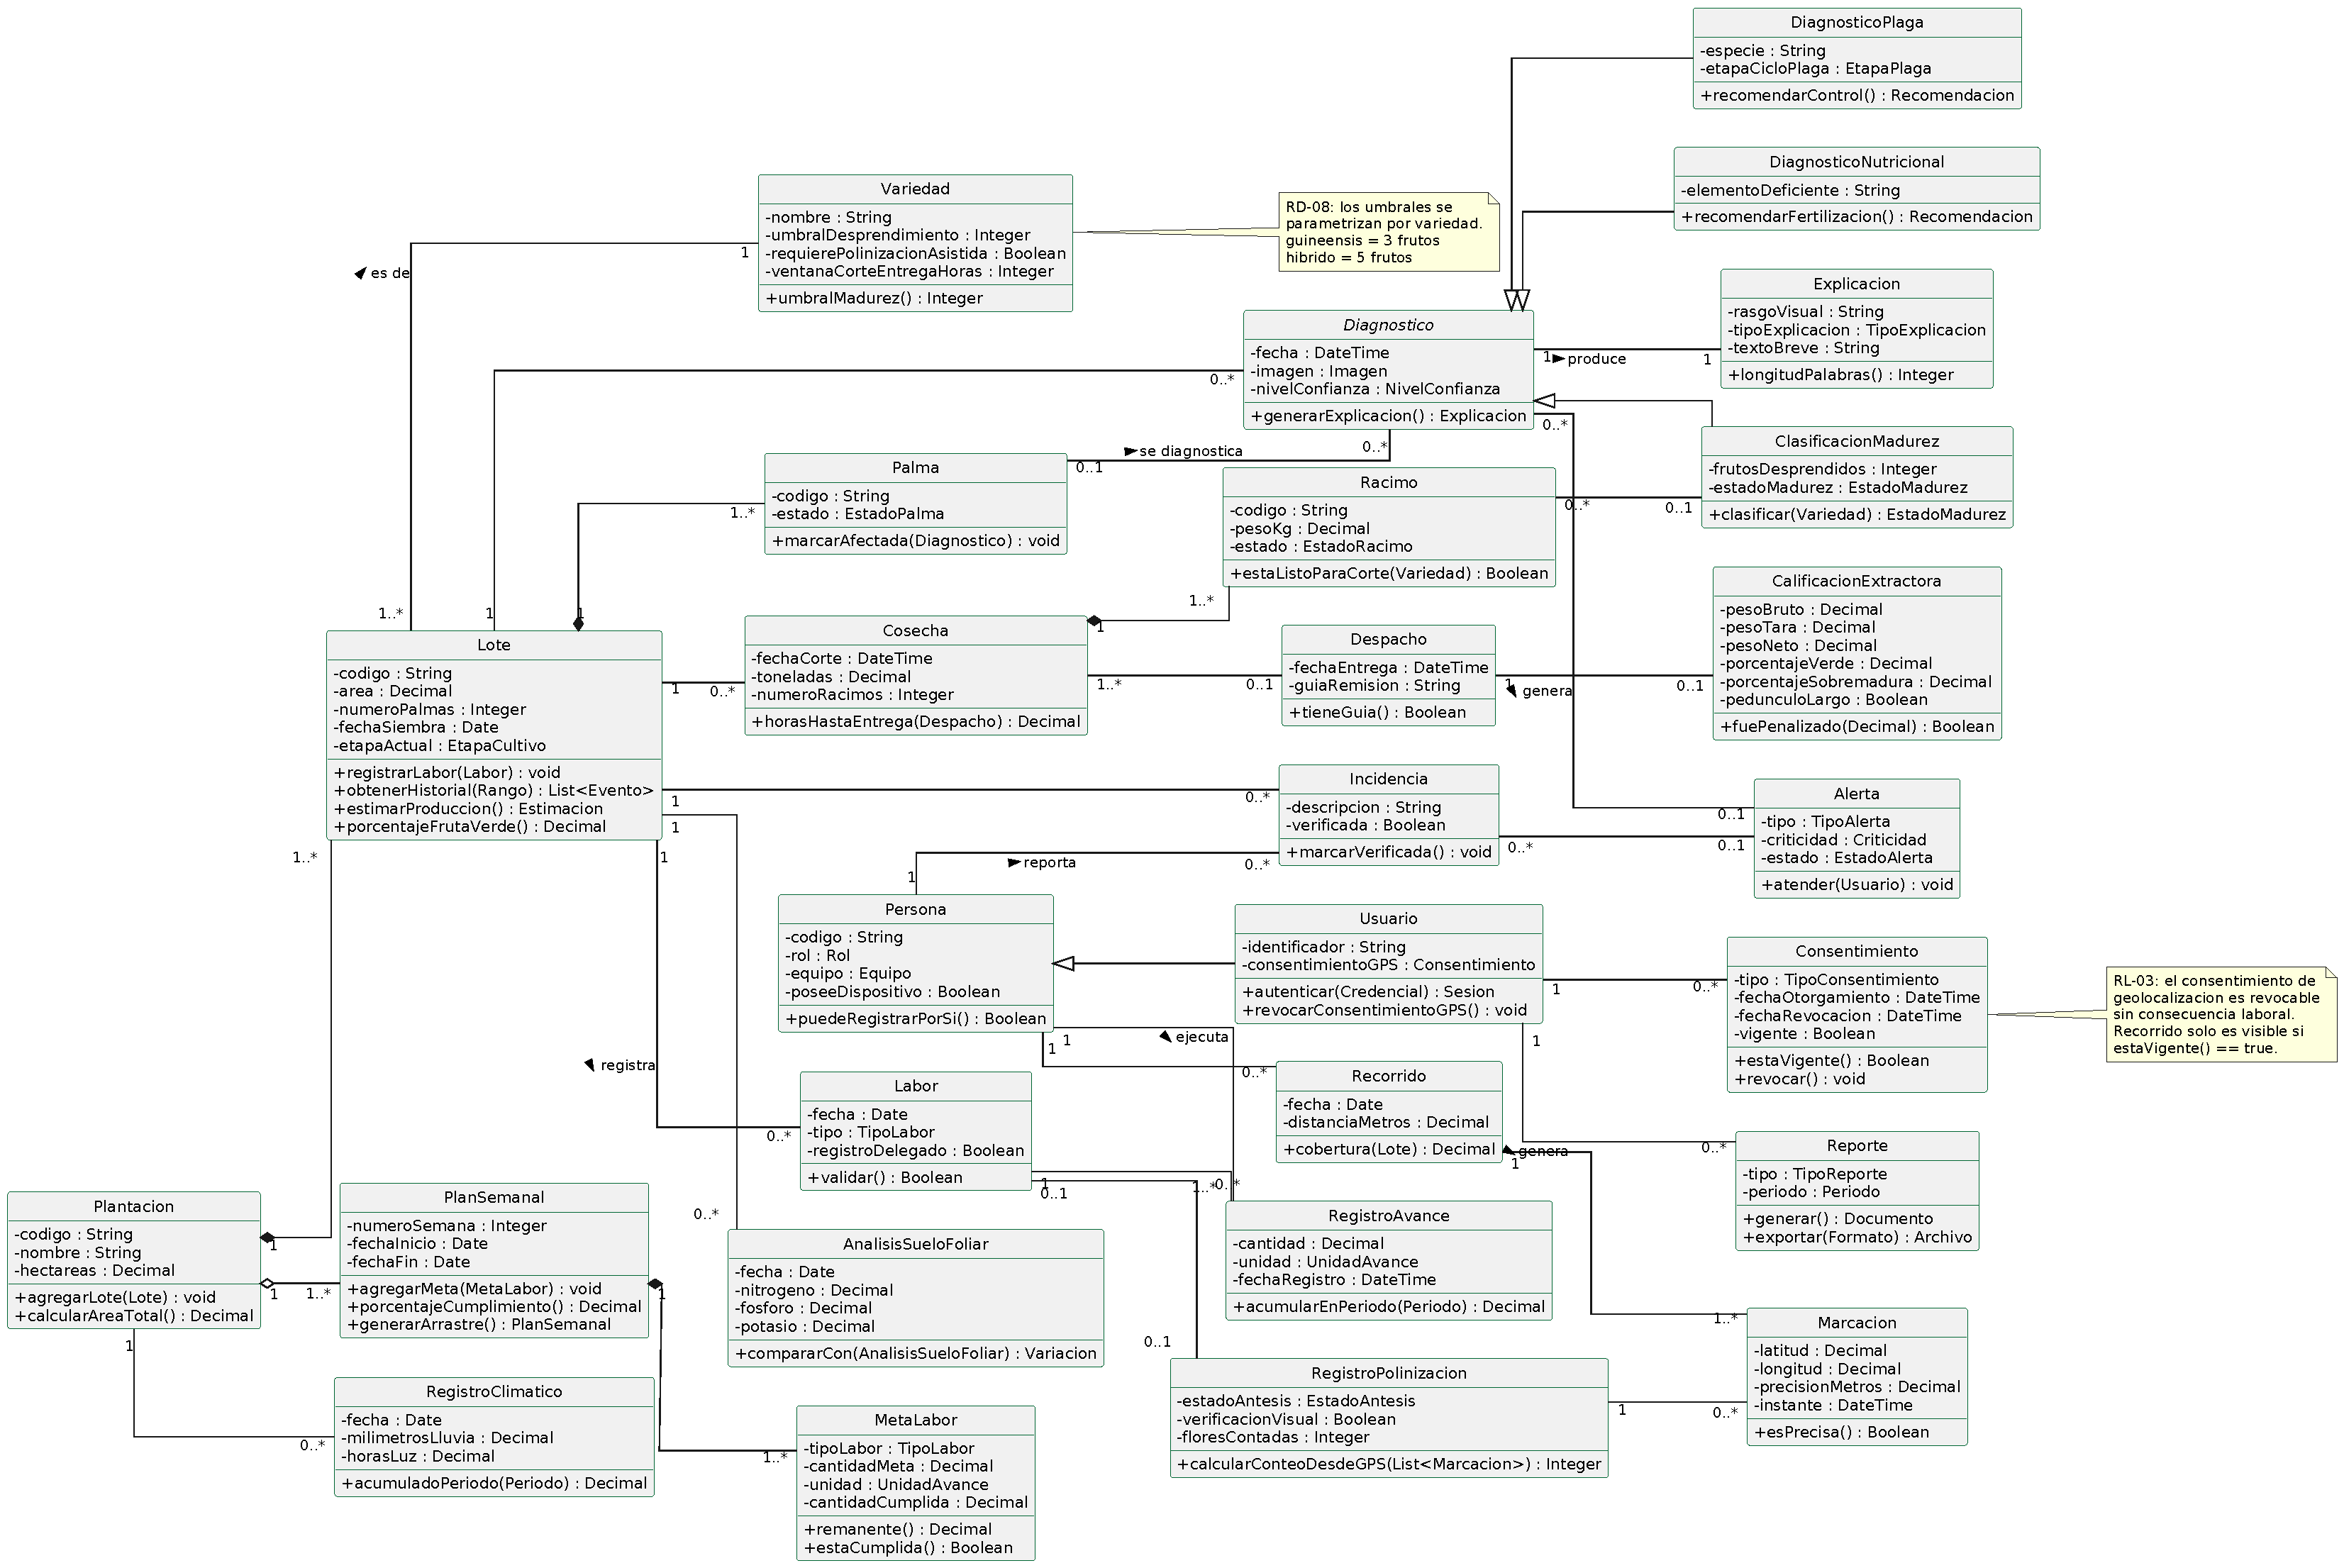
\includegraphics[width=1.0\textwidth]{img/clases_refinado}
\caption{Diagrama de clases refinado del SIMPA, con atributos y operaciones.}
\label{fig:clases}
\end{figure}

\noindent\textbf{Decisiones de modelado relevantes.} La clase \id{Consentimiento} se modela como
entidad de primer orden y no como atributo booleano de \id{Usuario}, porque el Art. 7 de la LOPDP
exige que el consentimiento sea específico por finalidad y revocable, lo que obliga a conservar su
historia. La clase \id{Variedad} concentra los umbrales de decisión ---desprendimiento, ventana
corte-entrega y necesidad de polinización asistida--- en lugar de fijarlos en la lógica de los
módulos de IA, conforme a \id{RD-08}. La clase \id{Explicacion} se asocia de forma obligatoria a
\id{Diagnostico} con multiplicidad 1:1, de modo que el modelo impide estructuralmente la existencia
de una decisión automática sin explicación (\id{RNF-16}). La clase \id{RegistroAvance} se separa de
\id{Labor} porque una labor puede acumular avances de varias personas y días, patrón observado en
los documentos de planificación semanal (\id{EV-11}).

% ---------------------------------------------------------------------
\subsection{Diagramas de secuencia}

Se presentan los diagramas de secuencia de los tres casos de uso \emph{Must} de mayor complejidad
de interacción.

\begin{figure}[!htbp]
\centering
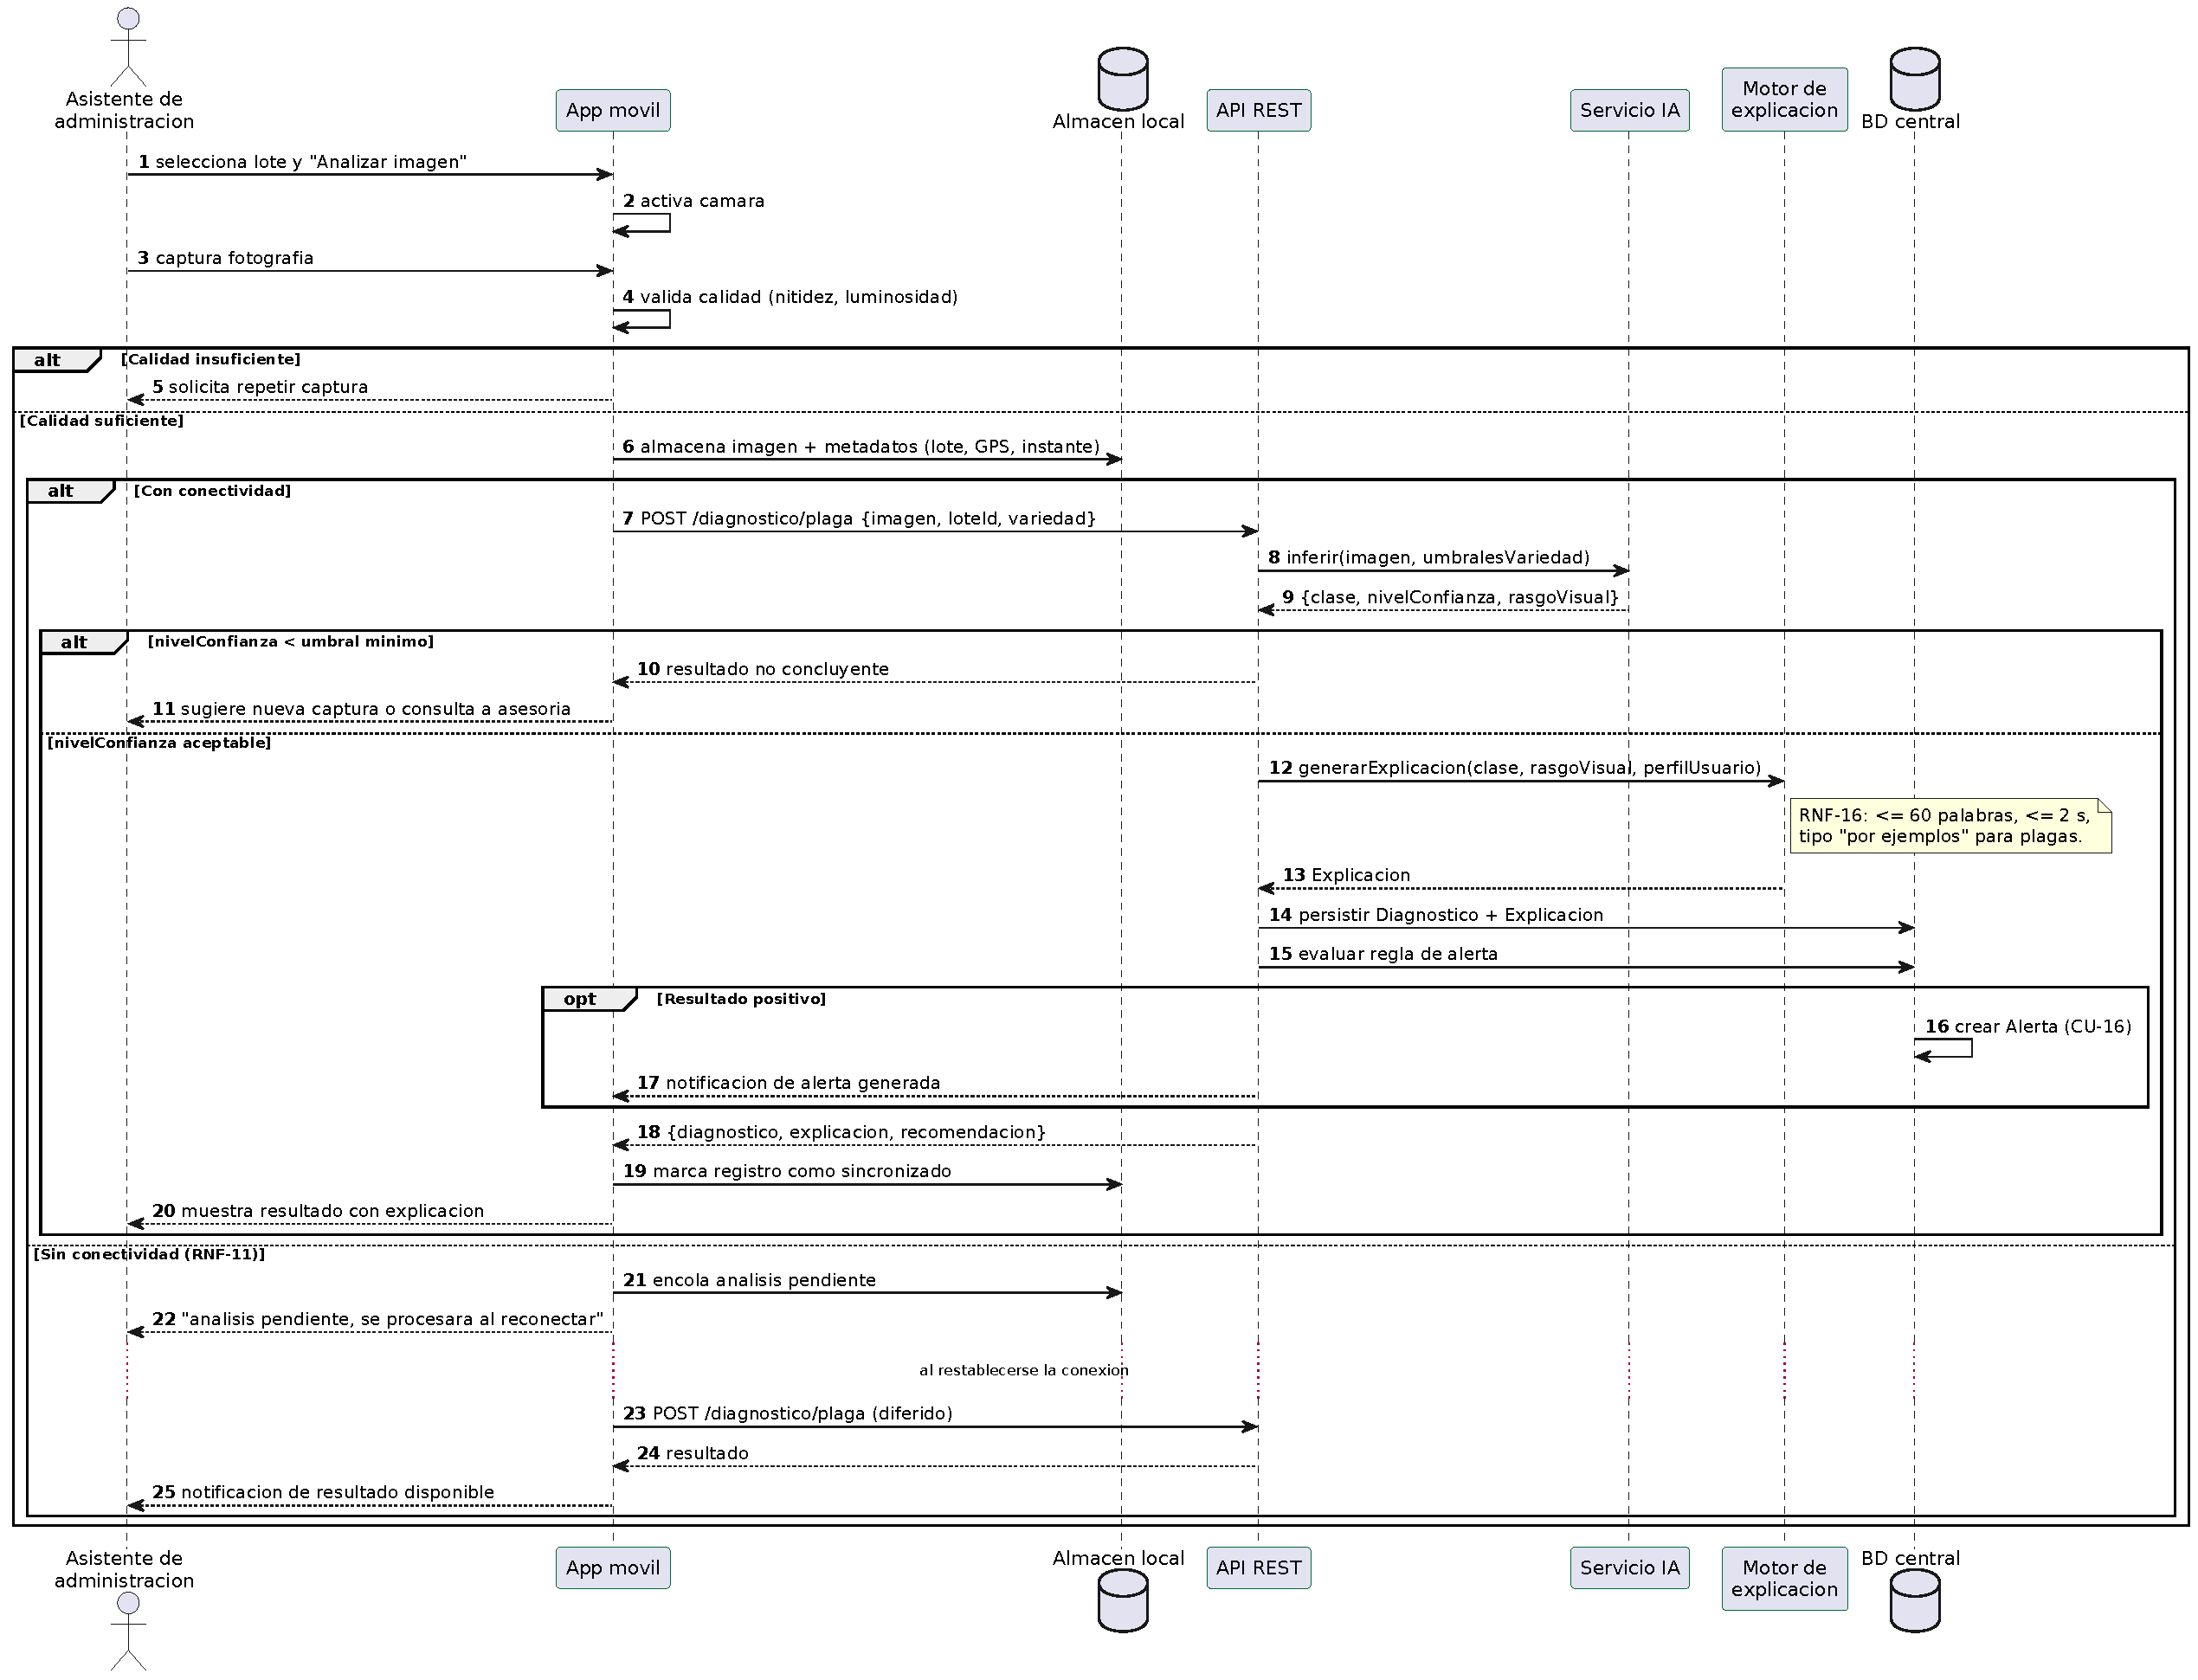
\includegraphics[width=1.0\textwidth]{img/secuencia_CU01}
\caption{Diagrama de secuencia del CU-01: análisis de imagen para detección de plaga, con las ramas de baja confianza y de operación sin conectividad.}
\label{fig:seq01}
\end{figure}

\begin{figure}[!htbp]
\centering
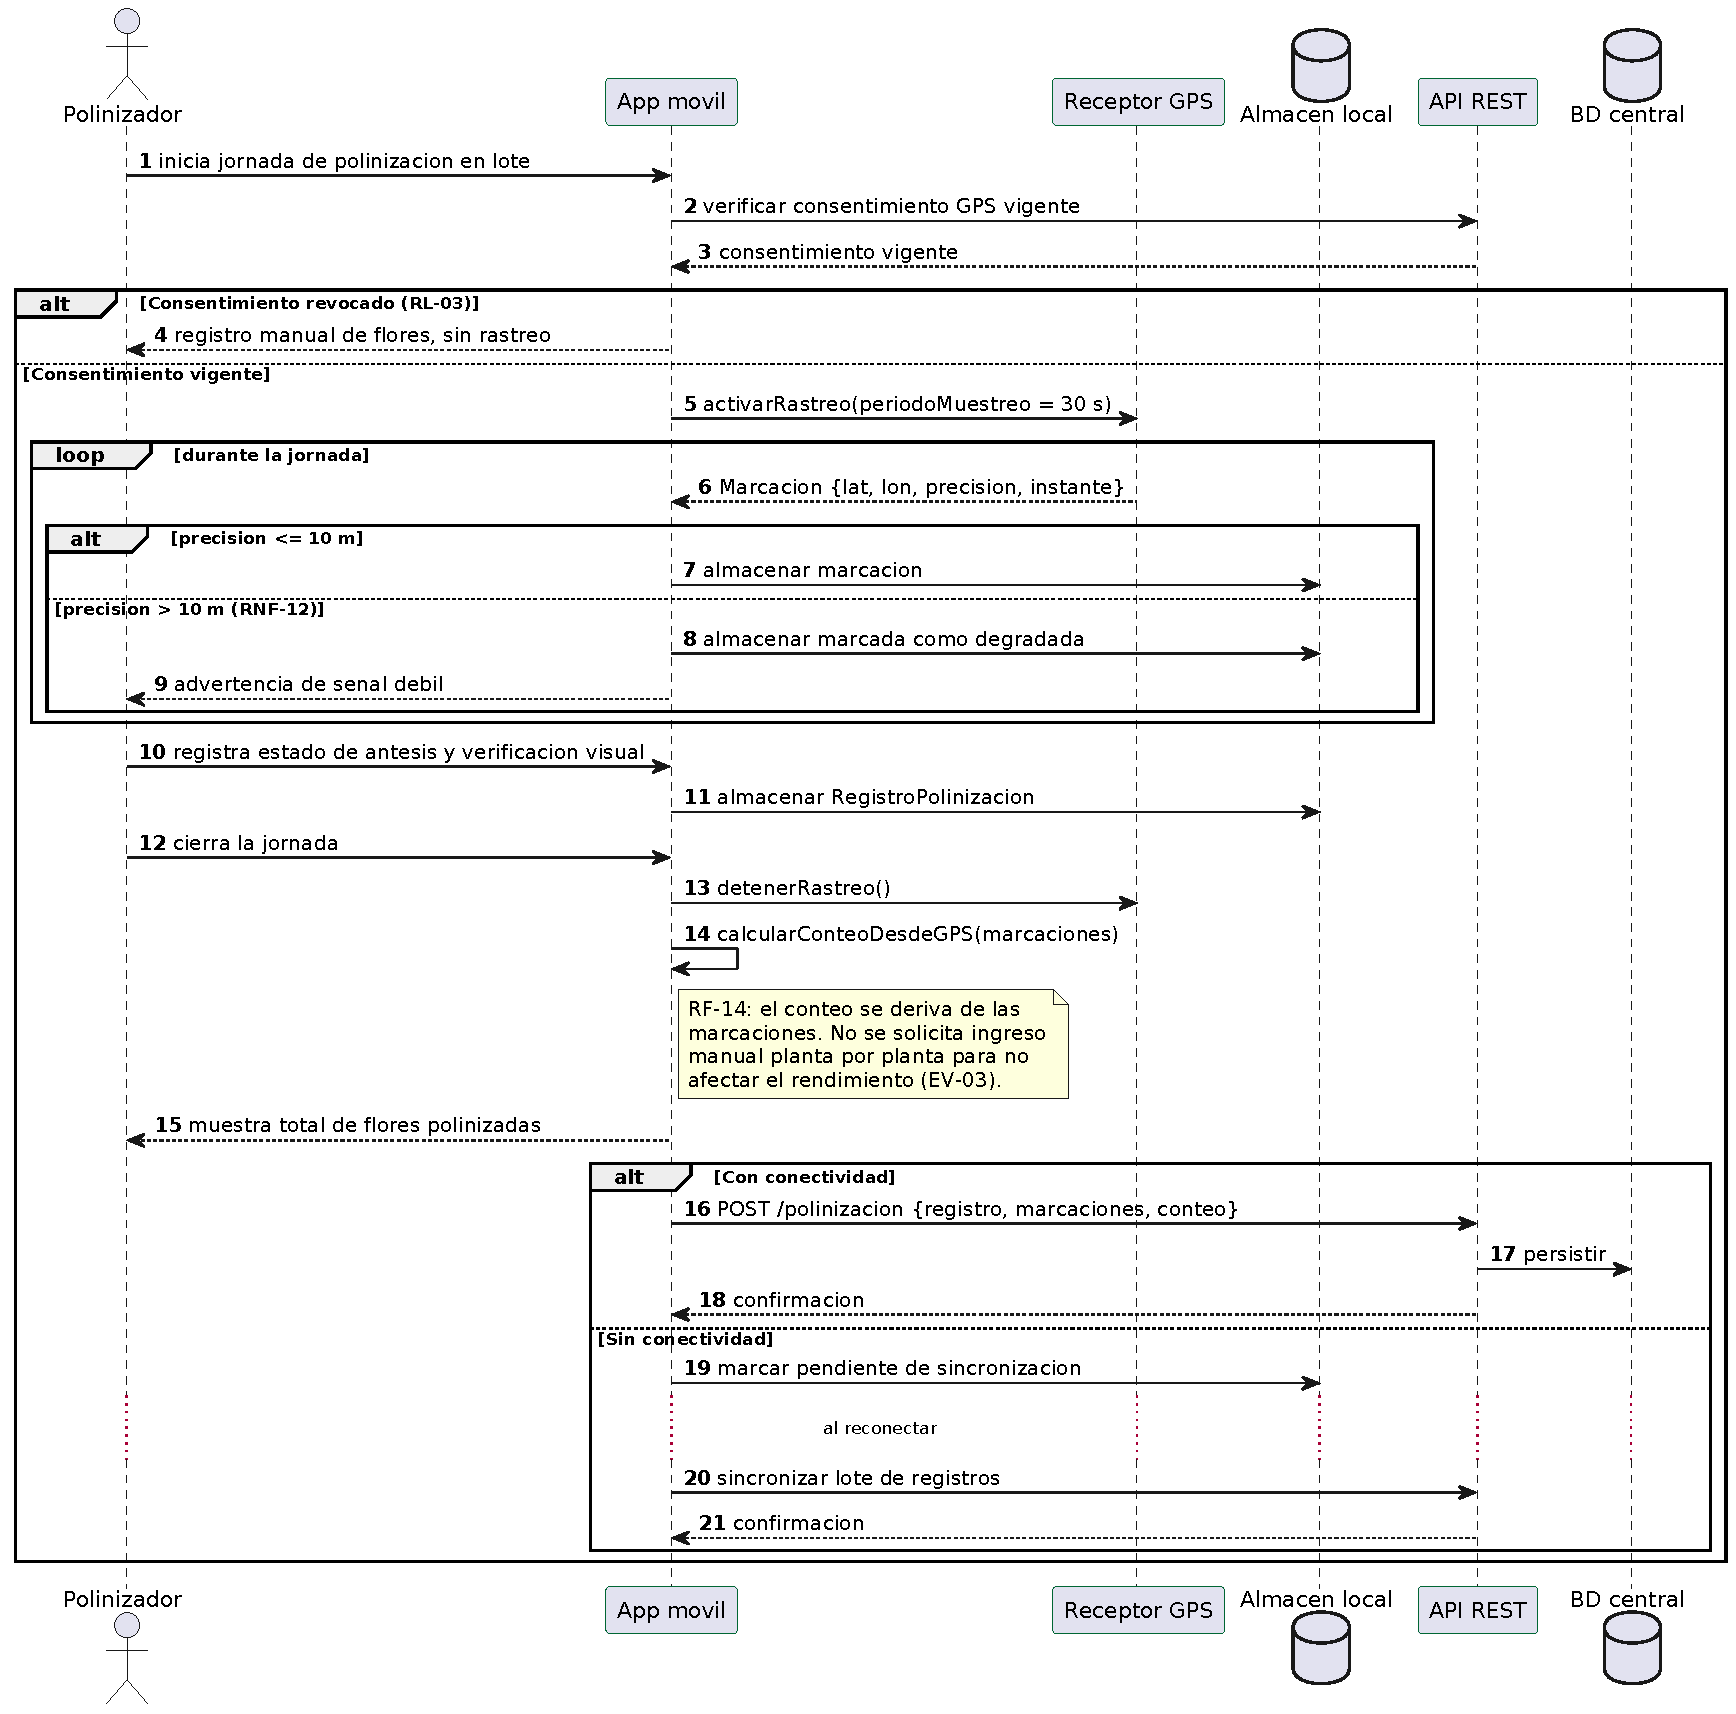
\includegraphics[width=1.0\textwidth]{img/secuencia_CU03}
\caption{Diagrama de secuencia del CU-03: registro de polinización y conteo georreferenciado, con verificación de consentimiento y manejo de precisión degradada.}
\label{fig:seq03}
\end{figure}

\begin{figure}[!htbp]
\centering
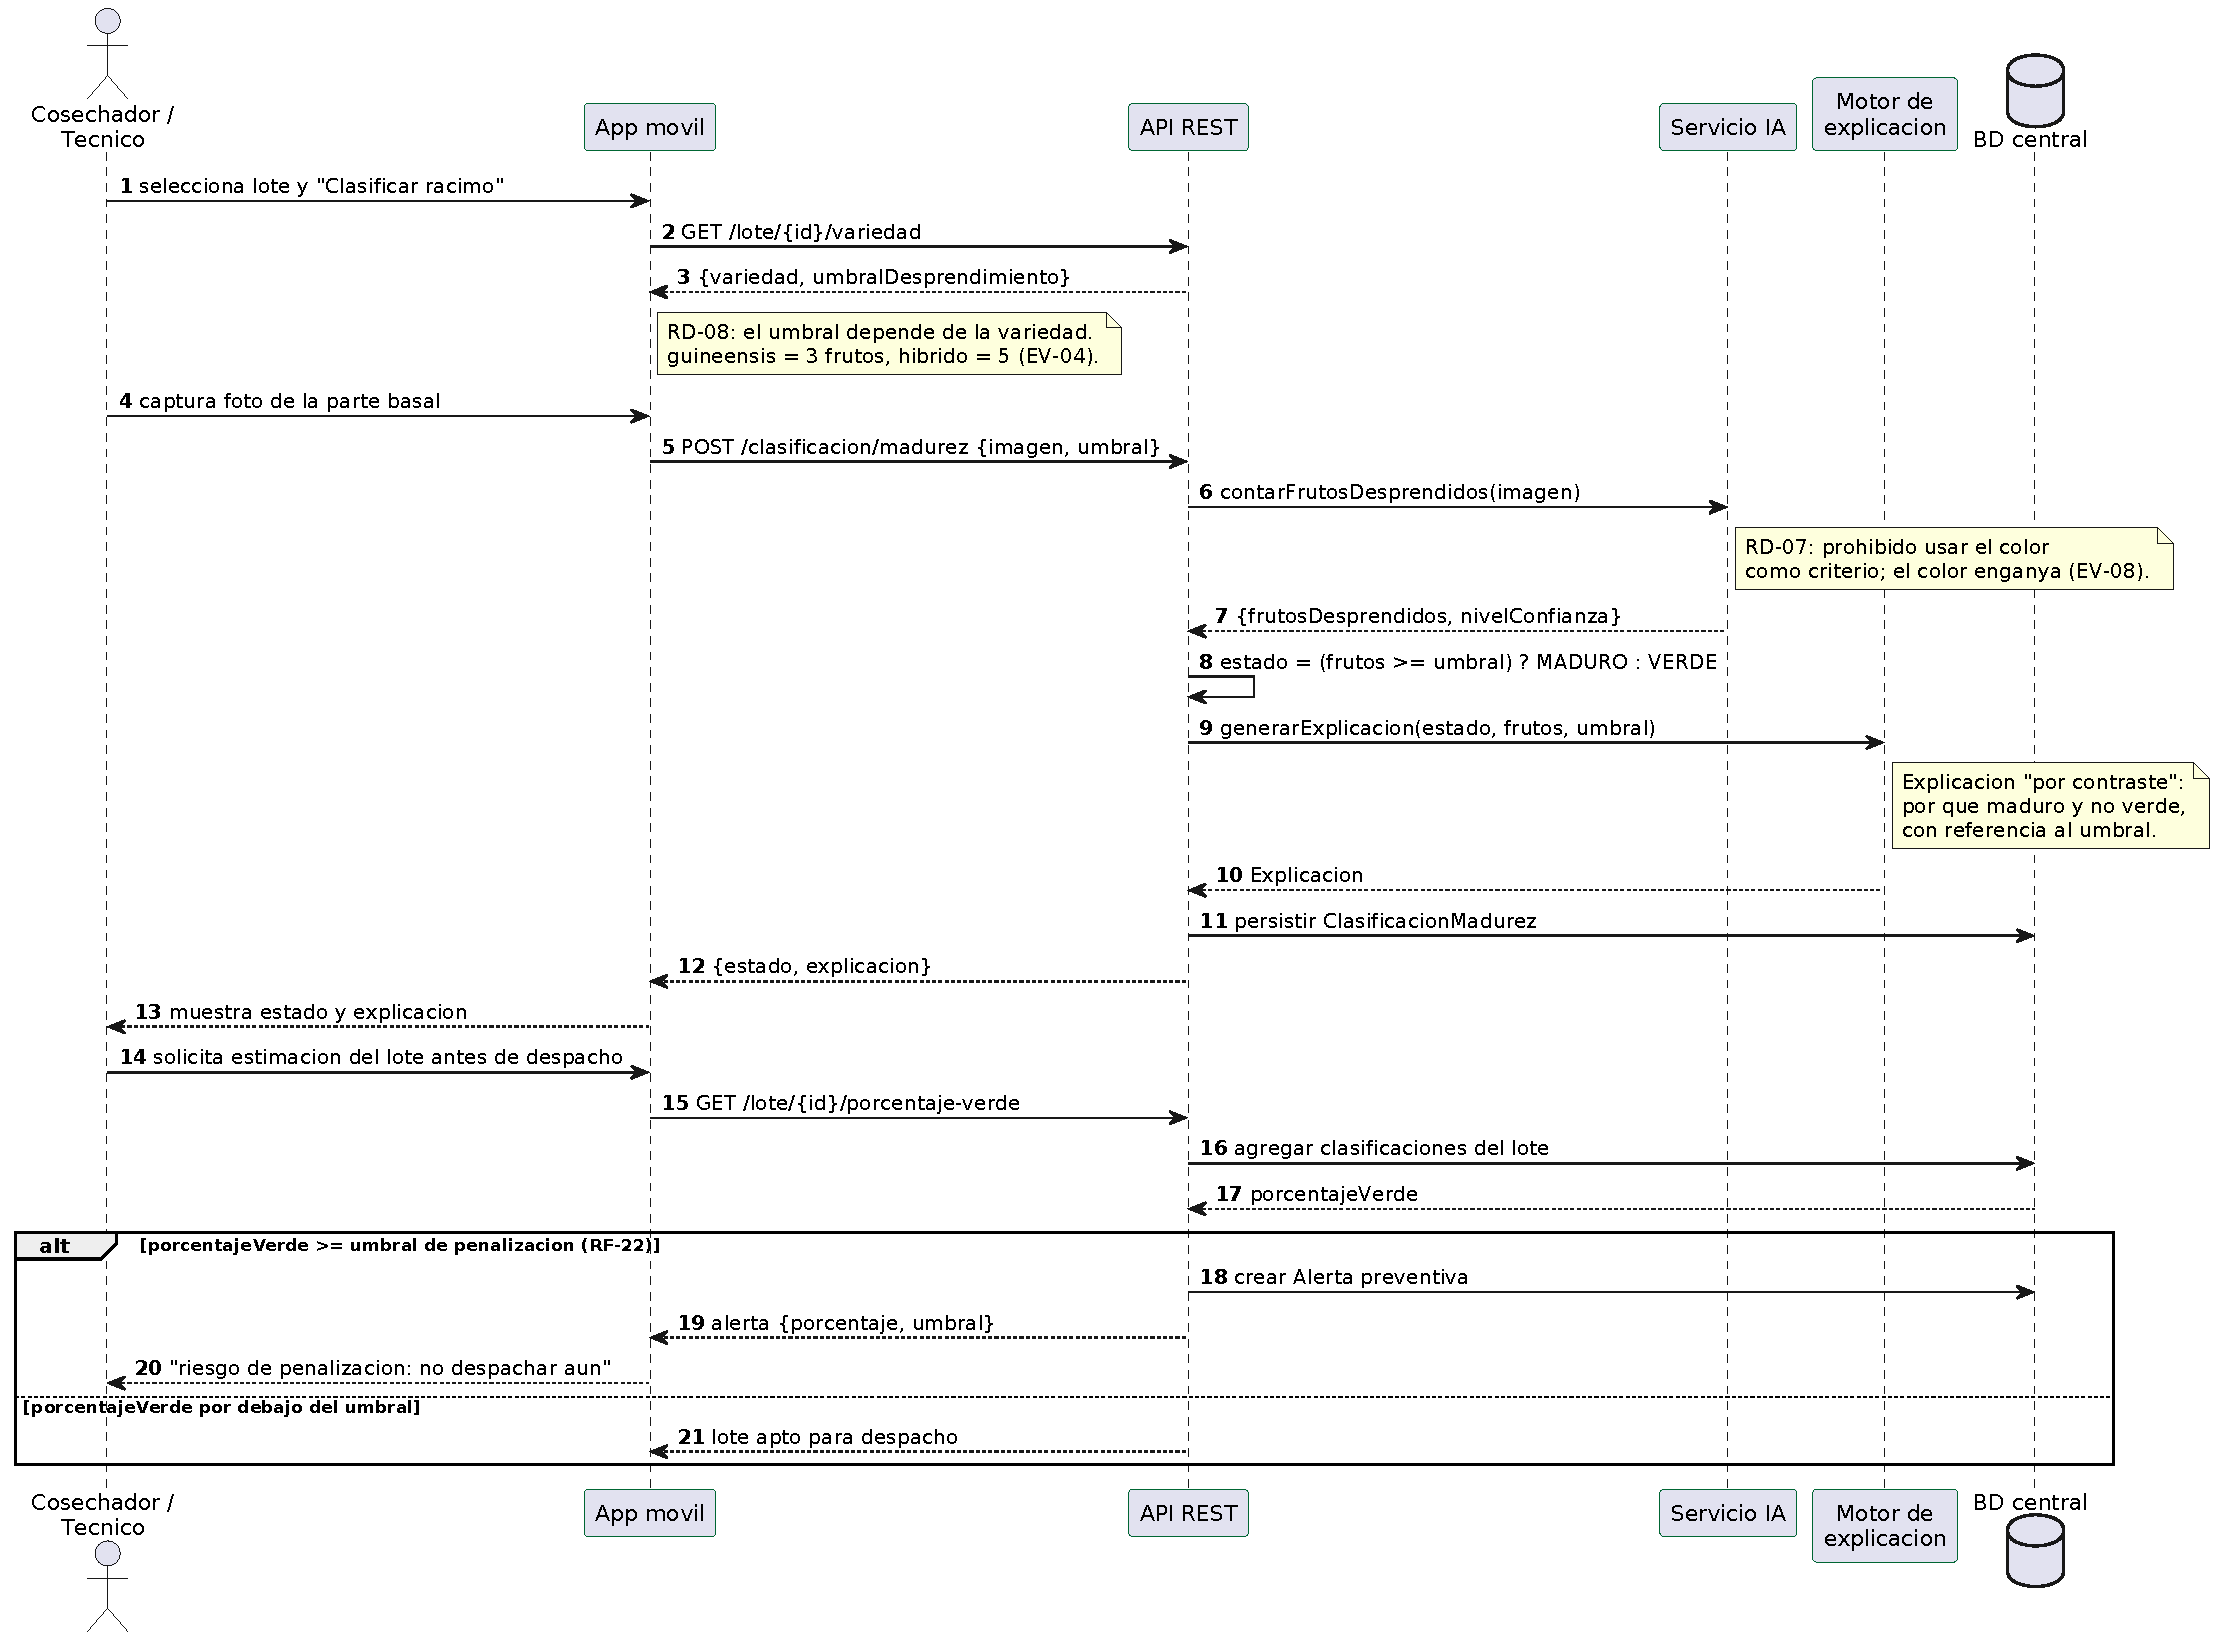
\includegraphics[width=1.0\textwidth]{img/secuencia_CU06}
\caption{Diagrama de secuencia del CU-06: clasificación de madurez del racimo y alerta preventiva de porcentaje de fruta verde.}
\label{fig:seq06}
\end{figure}

% ---------------------------------------------------------------------
\subsection{Diagrama de actividad}

El diagrama modela el ciclo semanal completo de planificación y ejecución, que constituye el proceso
central de la organización según los documentos operativos (\id{EV-11}). Incorpora la bifurcación
por disponibilidad de dispositivo (\id{RF-35}), la bifurcación por conectividad (\id{RNF-11}) y el
mecanismo de arrastre de labor incompleta (\id{RF-27}).

\begin{figure}[!htbp]
\centering
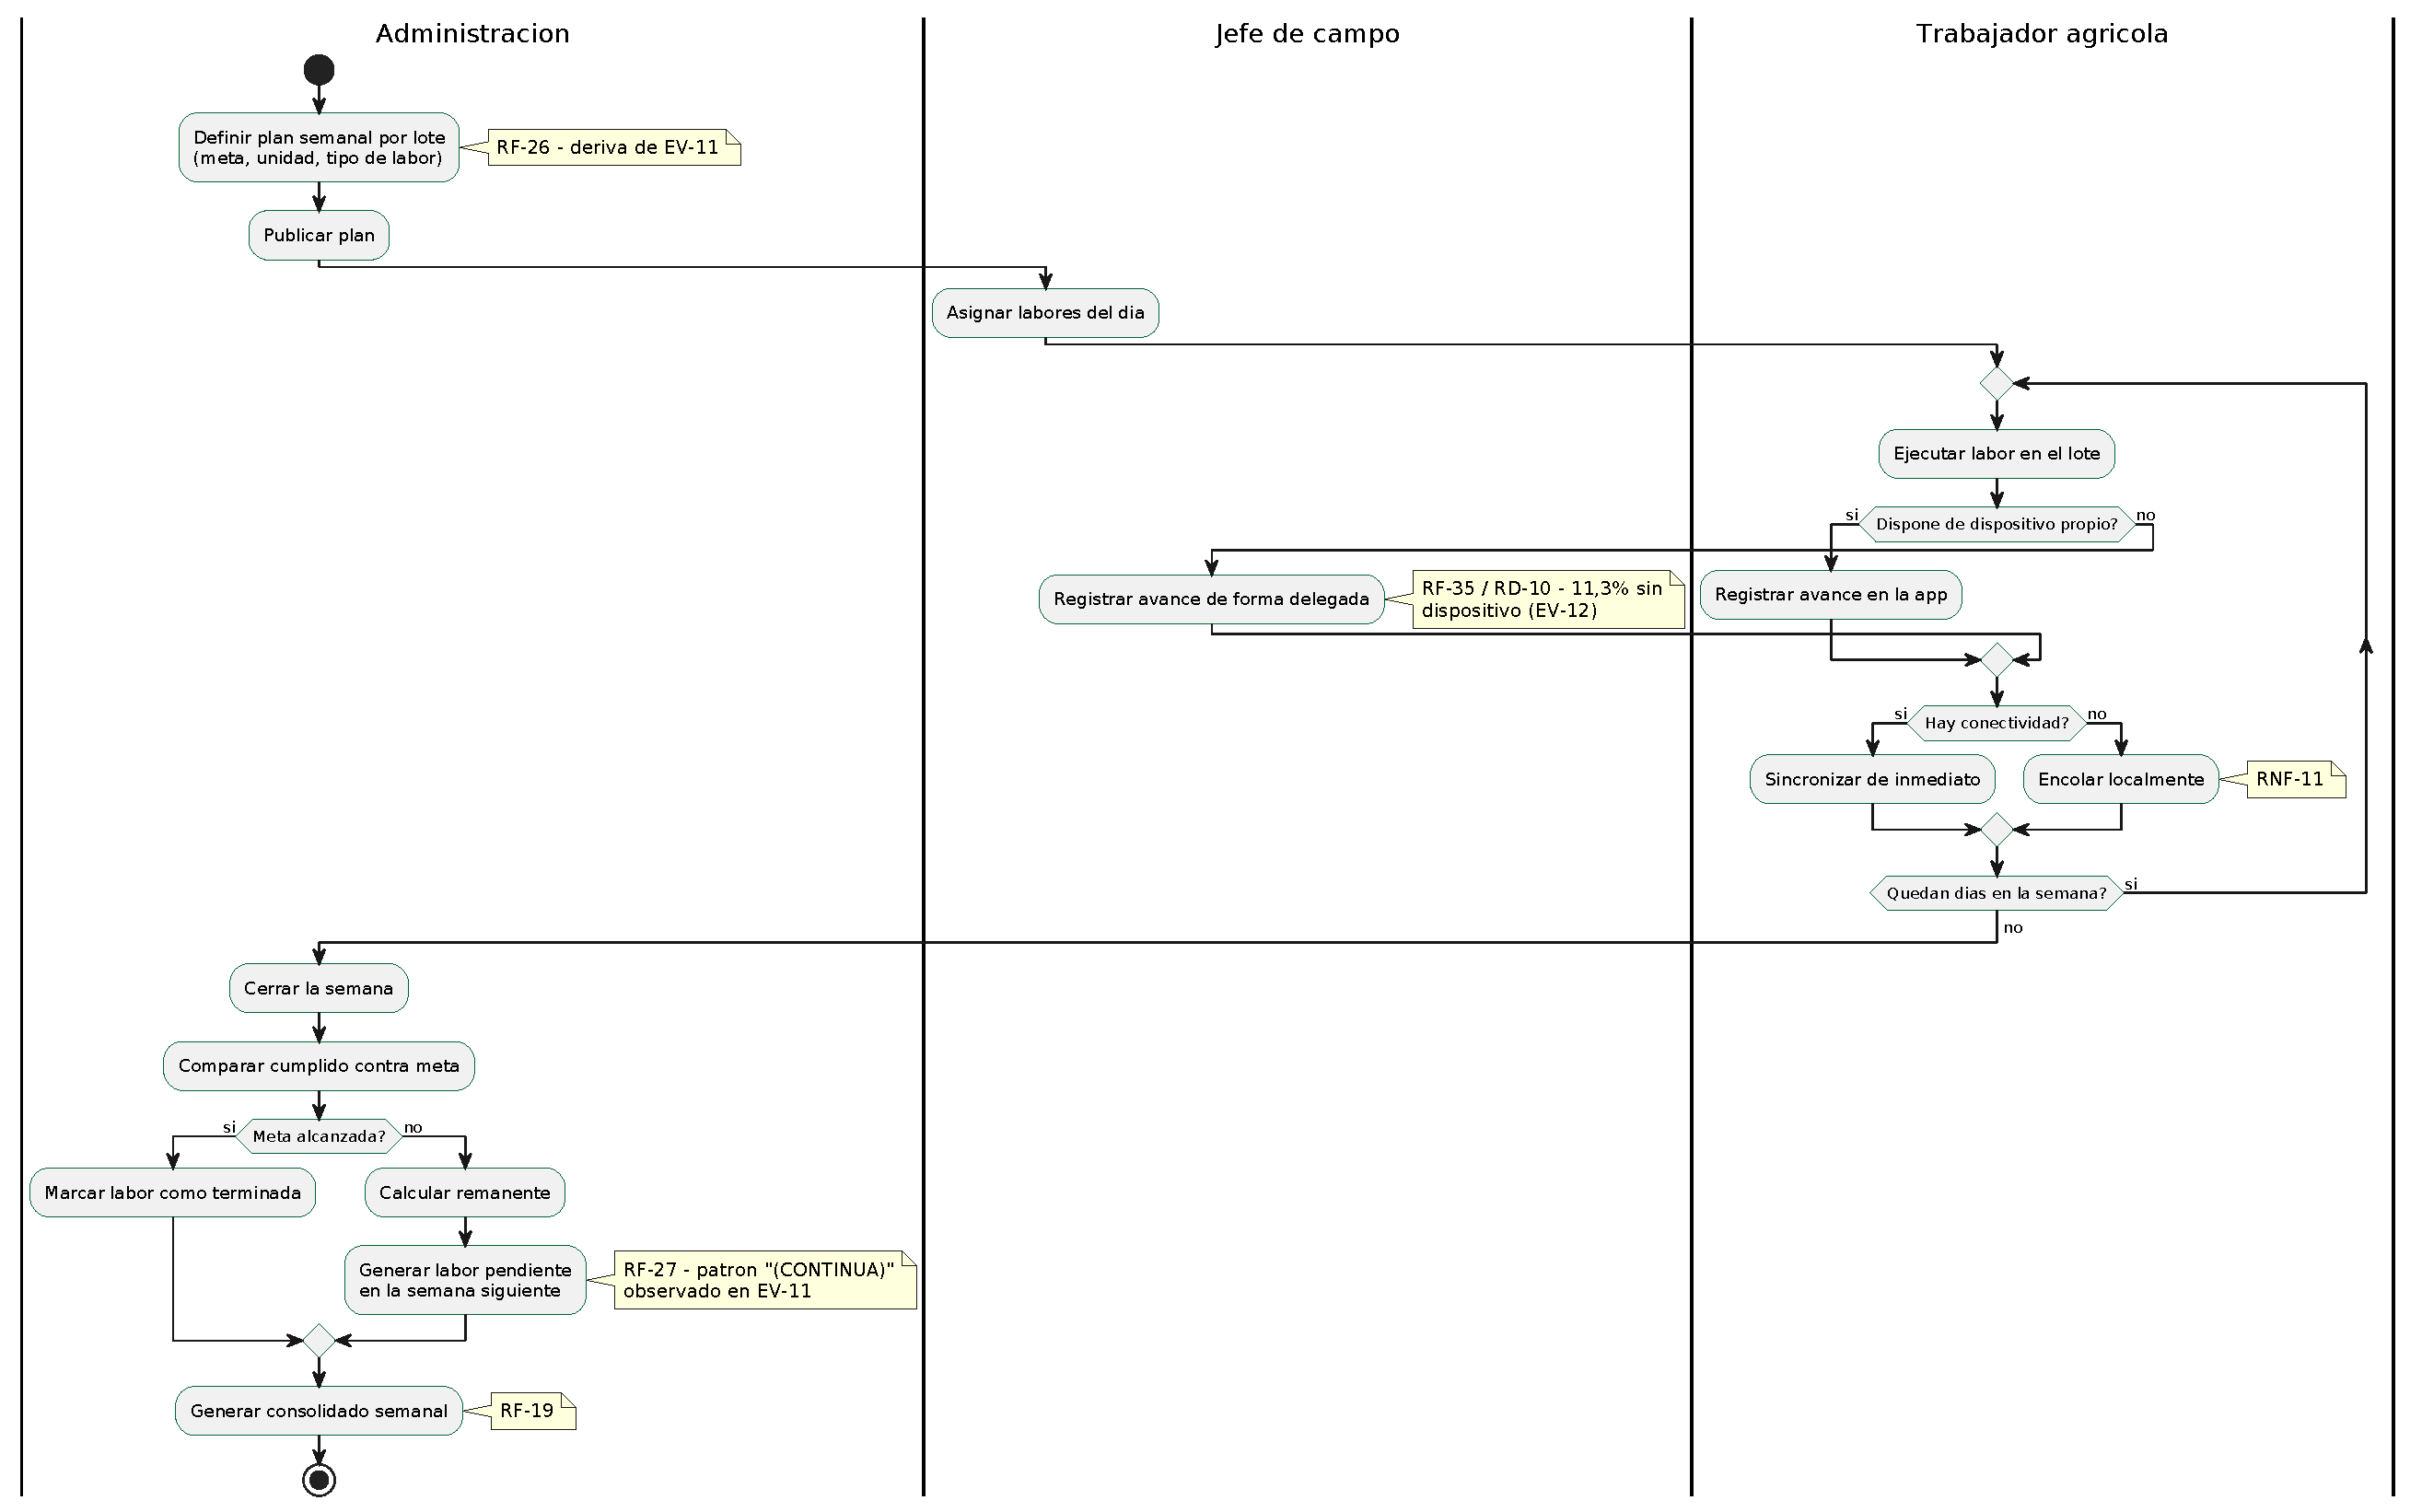
\includegraphics[width=1.0\textwidth]{img/actividad_ciclo_semanal}
\caption{Diagrama de actividad del ciclo semanal de planificación y ejecución de labores.}
\label{fig:actividad}
\end{figure}

% ---------------------------------------------------------------------
\subsection{Diagramas de estados}

Se modelan las dos entidades del dominio con ciclo de vida no trivial: el \textbf{racimo}, cuya
trayectoria determina el valor económico de la producción, y la \textbf{alerta}, cuyo ciclo refleja
la latencia real de verificación documentada en \id{EV-07}.

\begin{figure}[!htbp]
\centering
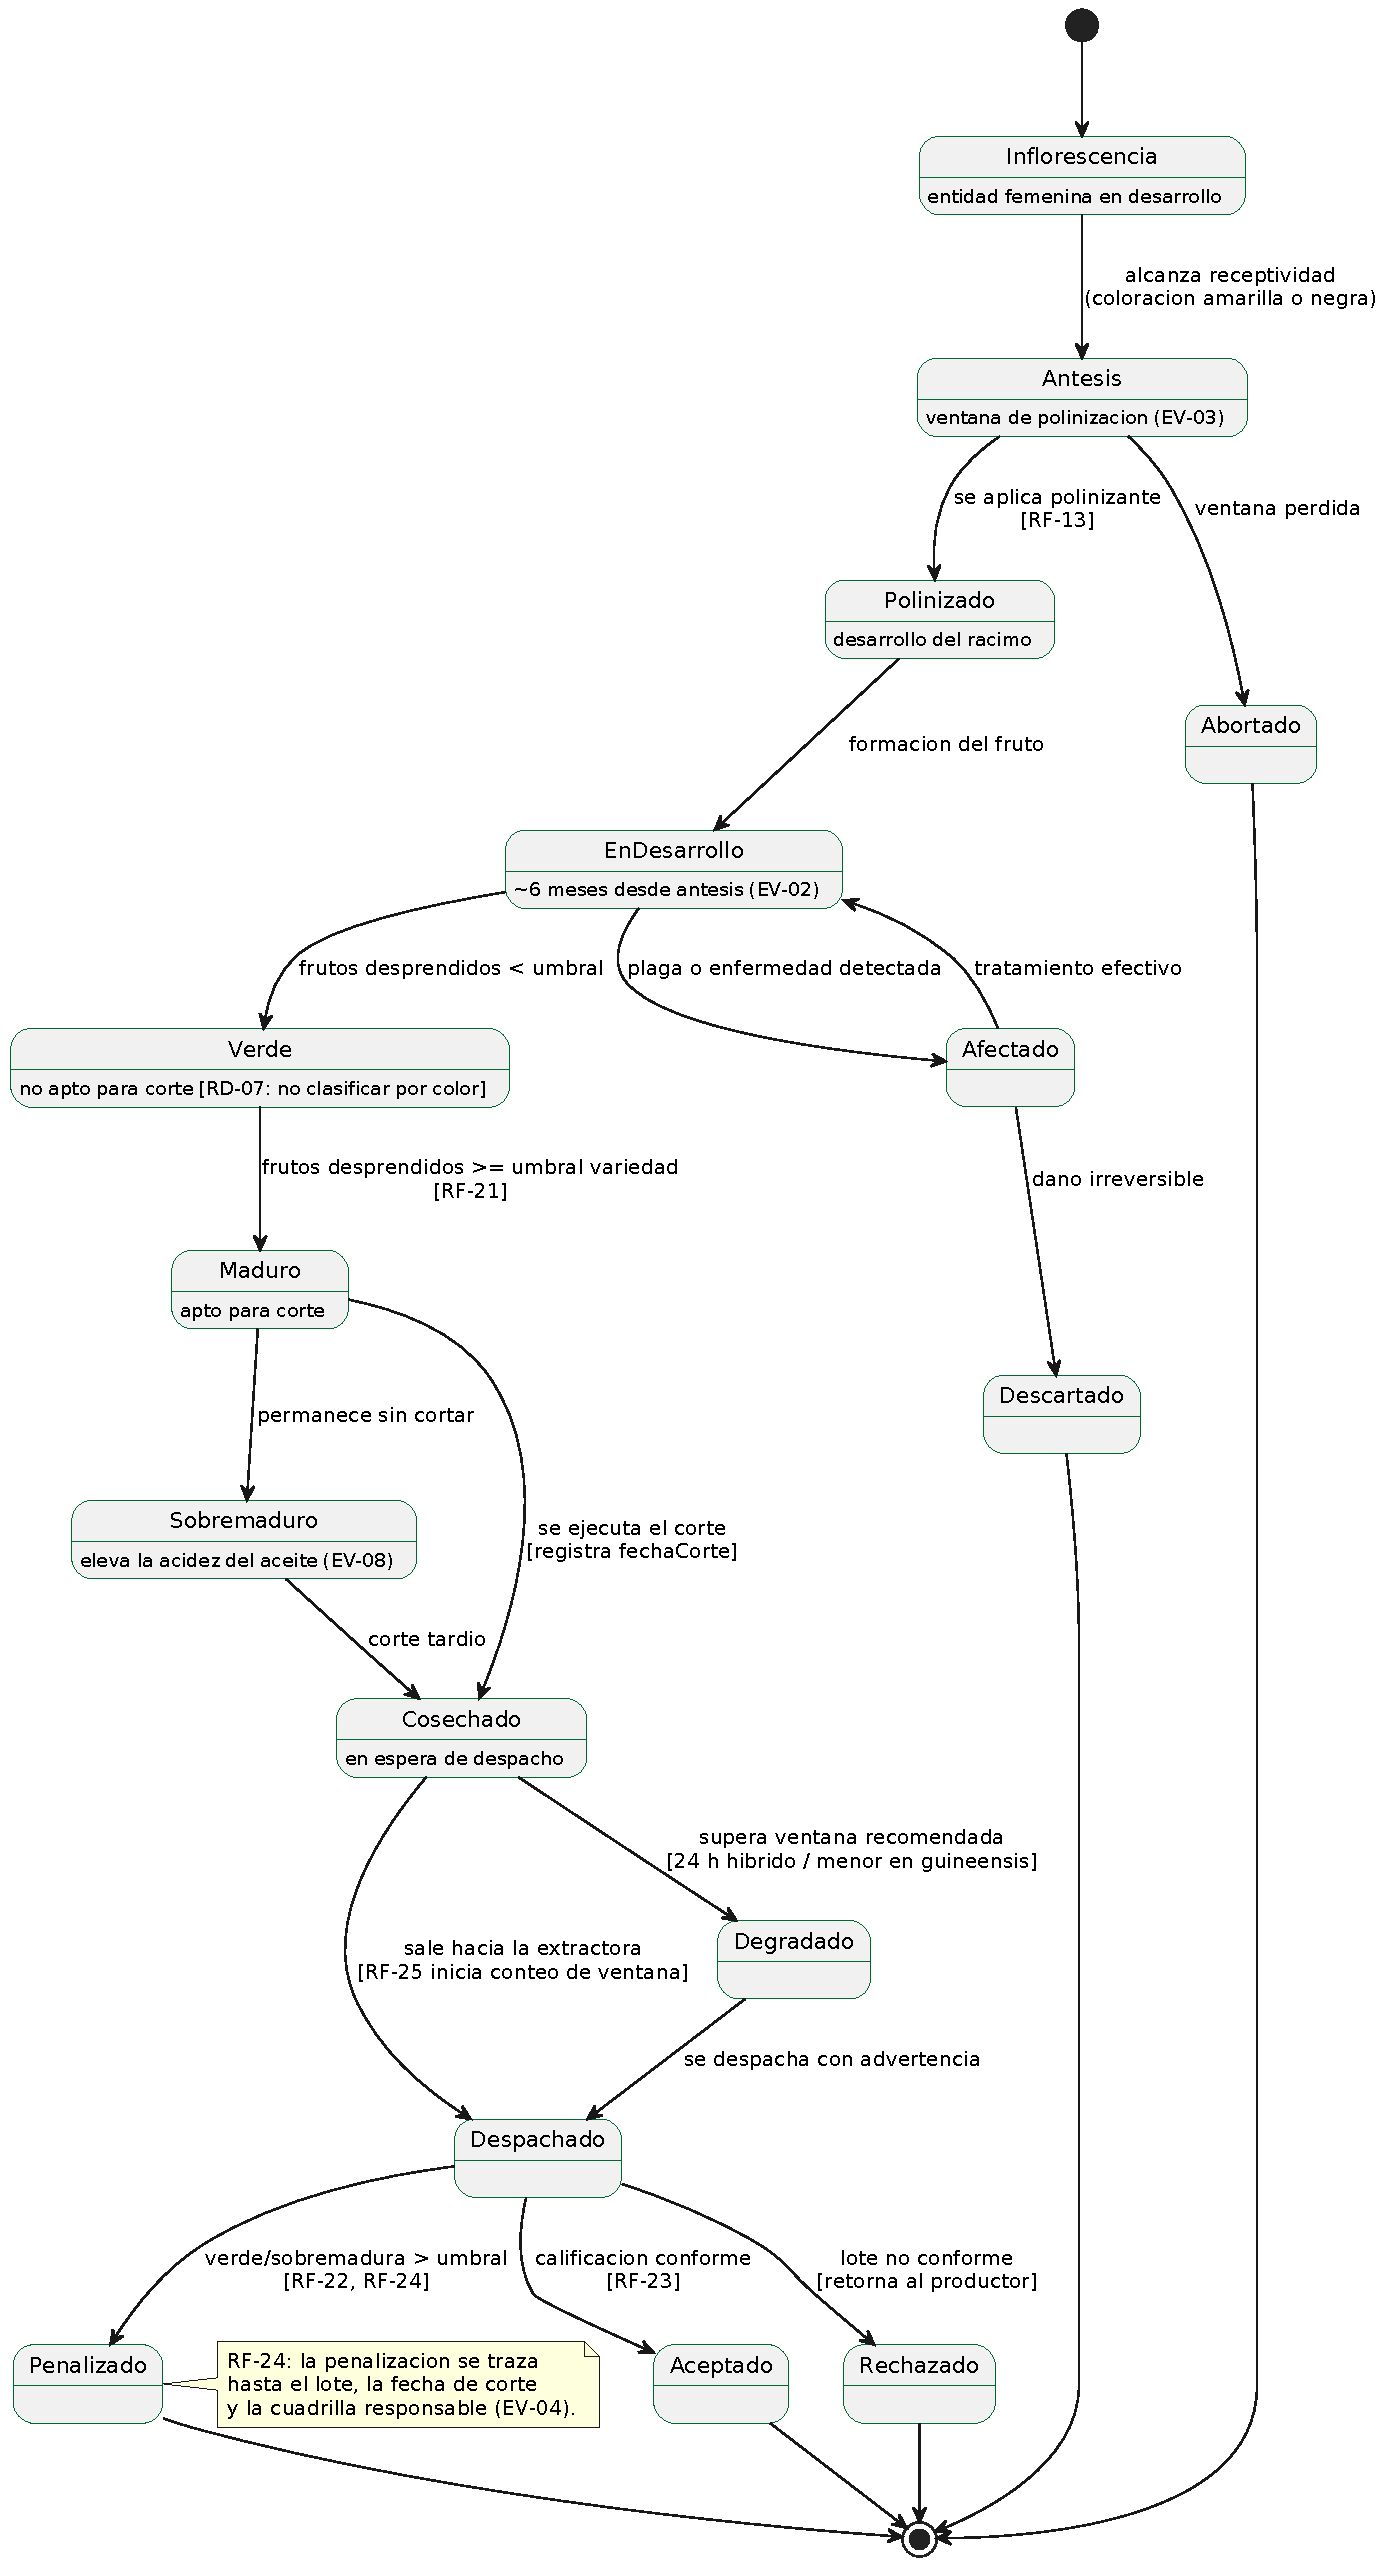
\includegraphics[width=0.67\textwidth]{img/estados_racimo}
\caption{Diagrama de estados del racimo, desde la inflorescencia hasta la calificación en la planta extractora.}
\label{fig:est_racimo}
\end{figure}

\begin{figure}[!htbp]
\centering
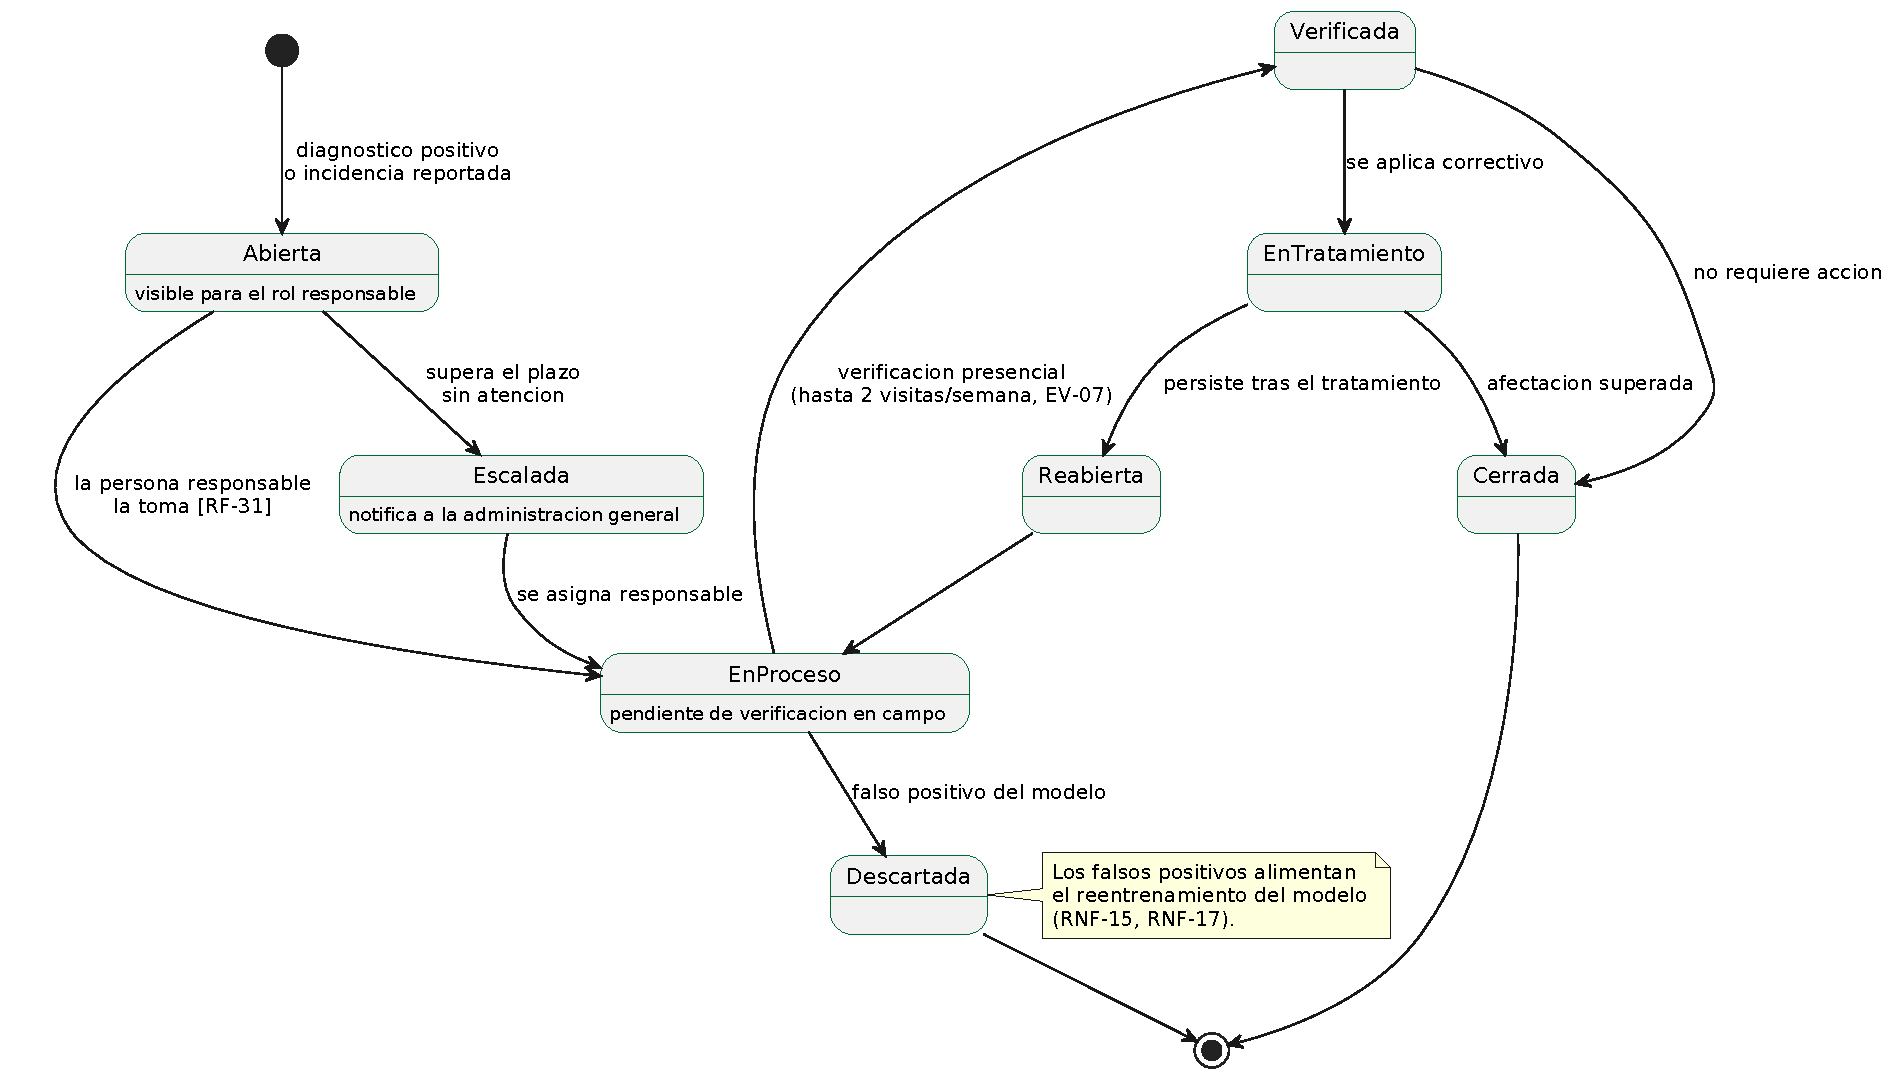
\includegraphics[width=1.0\textwidth]{img/estados_alerta}
\caption{Diagrama de estados de la alerta, con escalamiento por vencimiento de plazo y reapertura tras tratamiento inefectivo.}
\label{fig:est_alerta}
\end{figure}

\noindent
El estado \emph{Degradado} del racimo materializa el hallazgo de \id{EV-04} sobre la ventana entre
corte y entrega: el material híbrido tolera un intervalo mayor por su contenido de antioxidantes,
mientras que el \emph{guineensis} se deshidrata en dos o tres días. El estado \emph{Descartada} de
la alerta corresponde a los falsos positivos del modelo y alimenta el ciclo de reentrenamiento
previsto en \id{RNF-15} y \id{RNF-17}.

% ---------------------------------------------------------------------
\subsection{Diagrama de componentes}

\begin{figure}[!htbp]
\centering
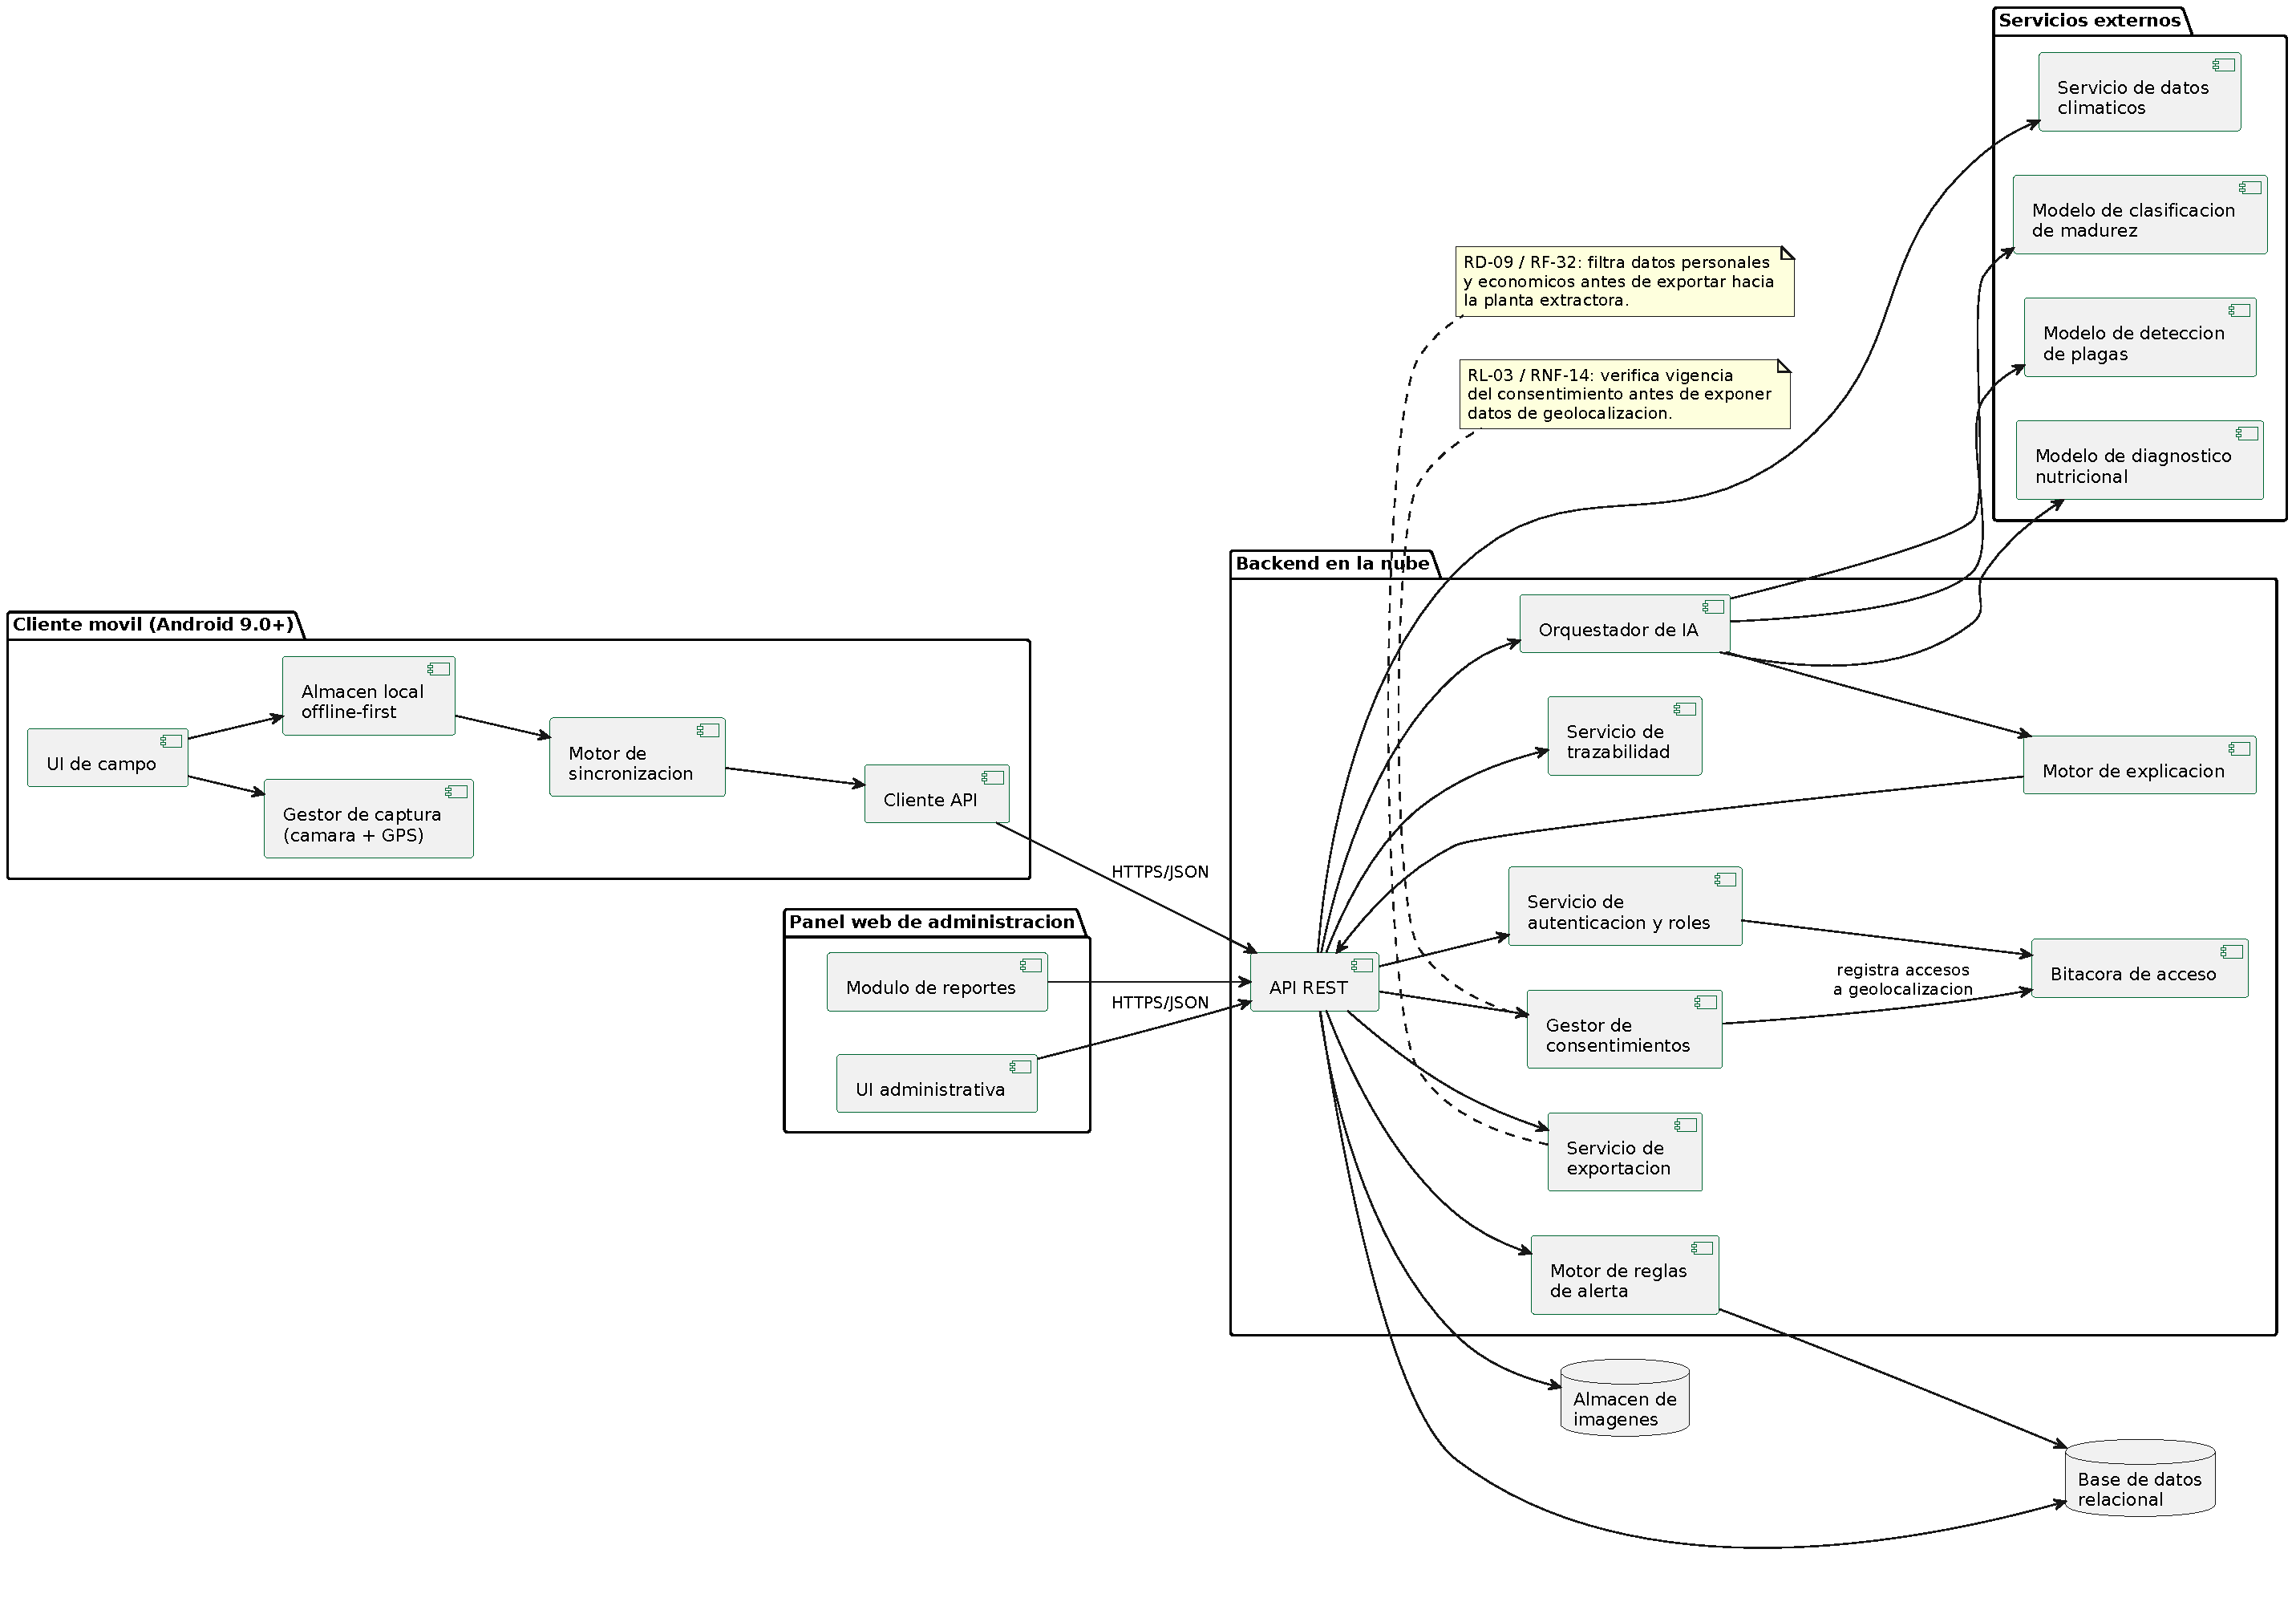
\includegraphics[width=1.0\textwidth]{img/componentes}
\caption{Diagrama de componentes del SIMPA.}
\label{fig:componentes}
\end{figure}

\noindent
Dos componentes merecen mención explícita por su origen normativo. El \emph{gestor de
consentimientos} verifica la vigencia antes de exponer cualquier dato de geolocalización y registra
todo acceso en la bitácora (\id{RL-03}, \id{RNF-14}). El \emph{servicio de exportación} filtra los
datos personales y económicos antes de generar el archivo destinado a la planta extractora
(\id{RD-09}, \id{RF-32}); su existencia como componente separado responde al criterio expreso de la
contraparte de que hay información que no puede compartirse (\id{EV-04}).

% ---------------------------------------------------------------------
\subsection{Diagrama de despliegue}

\begin{figure}[!htbp]
\centering
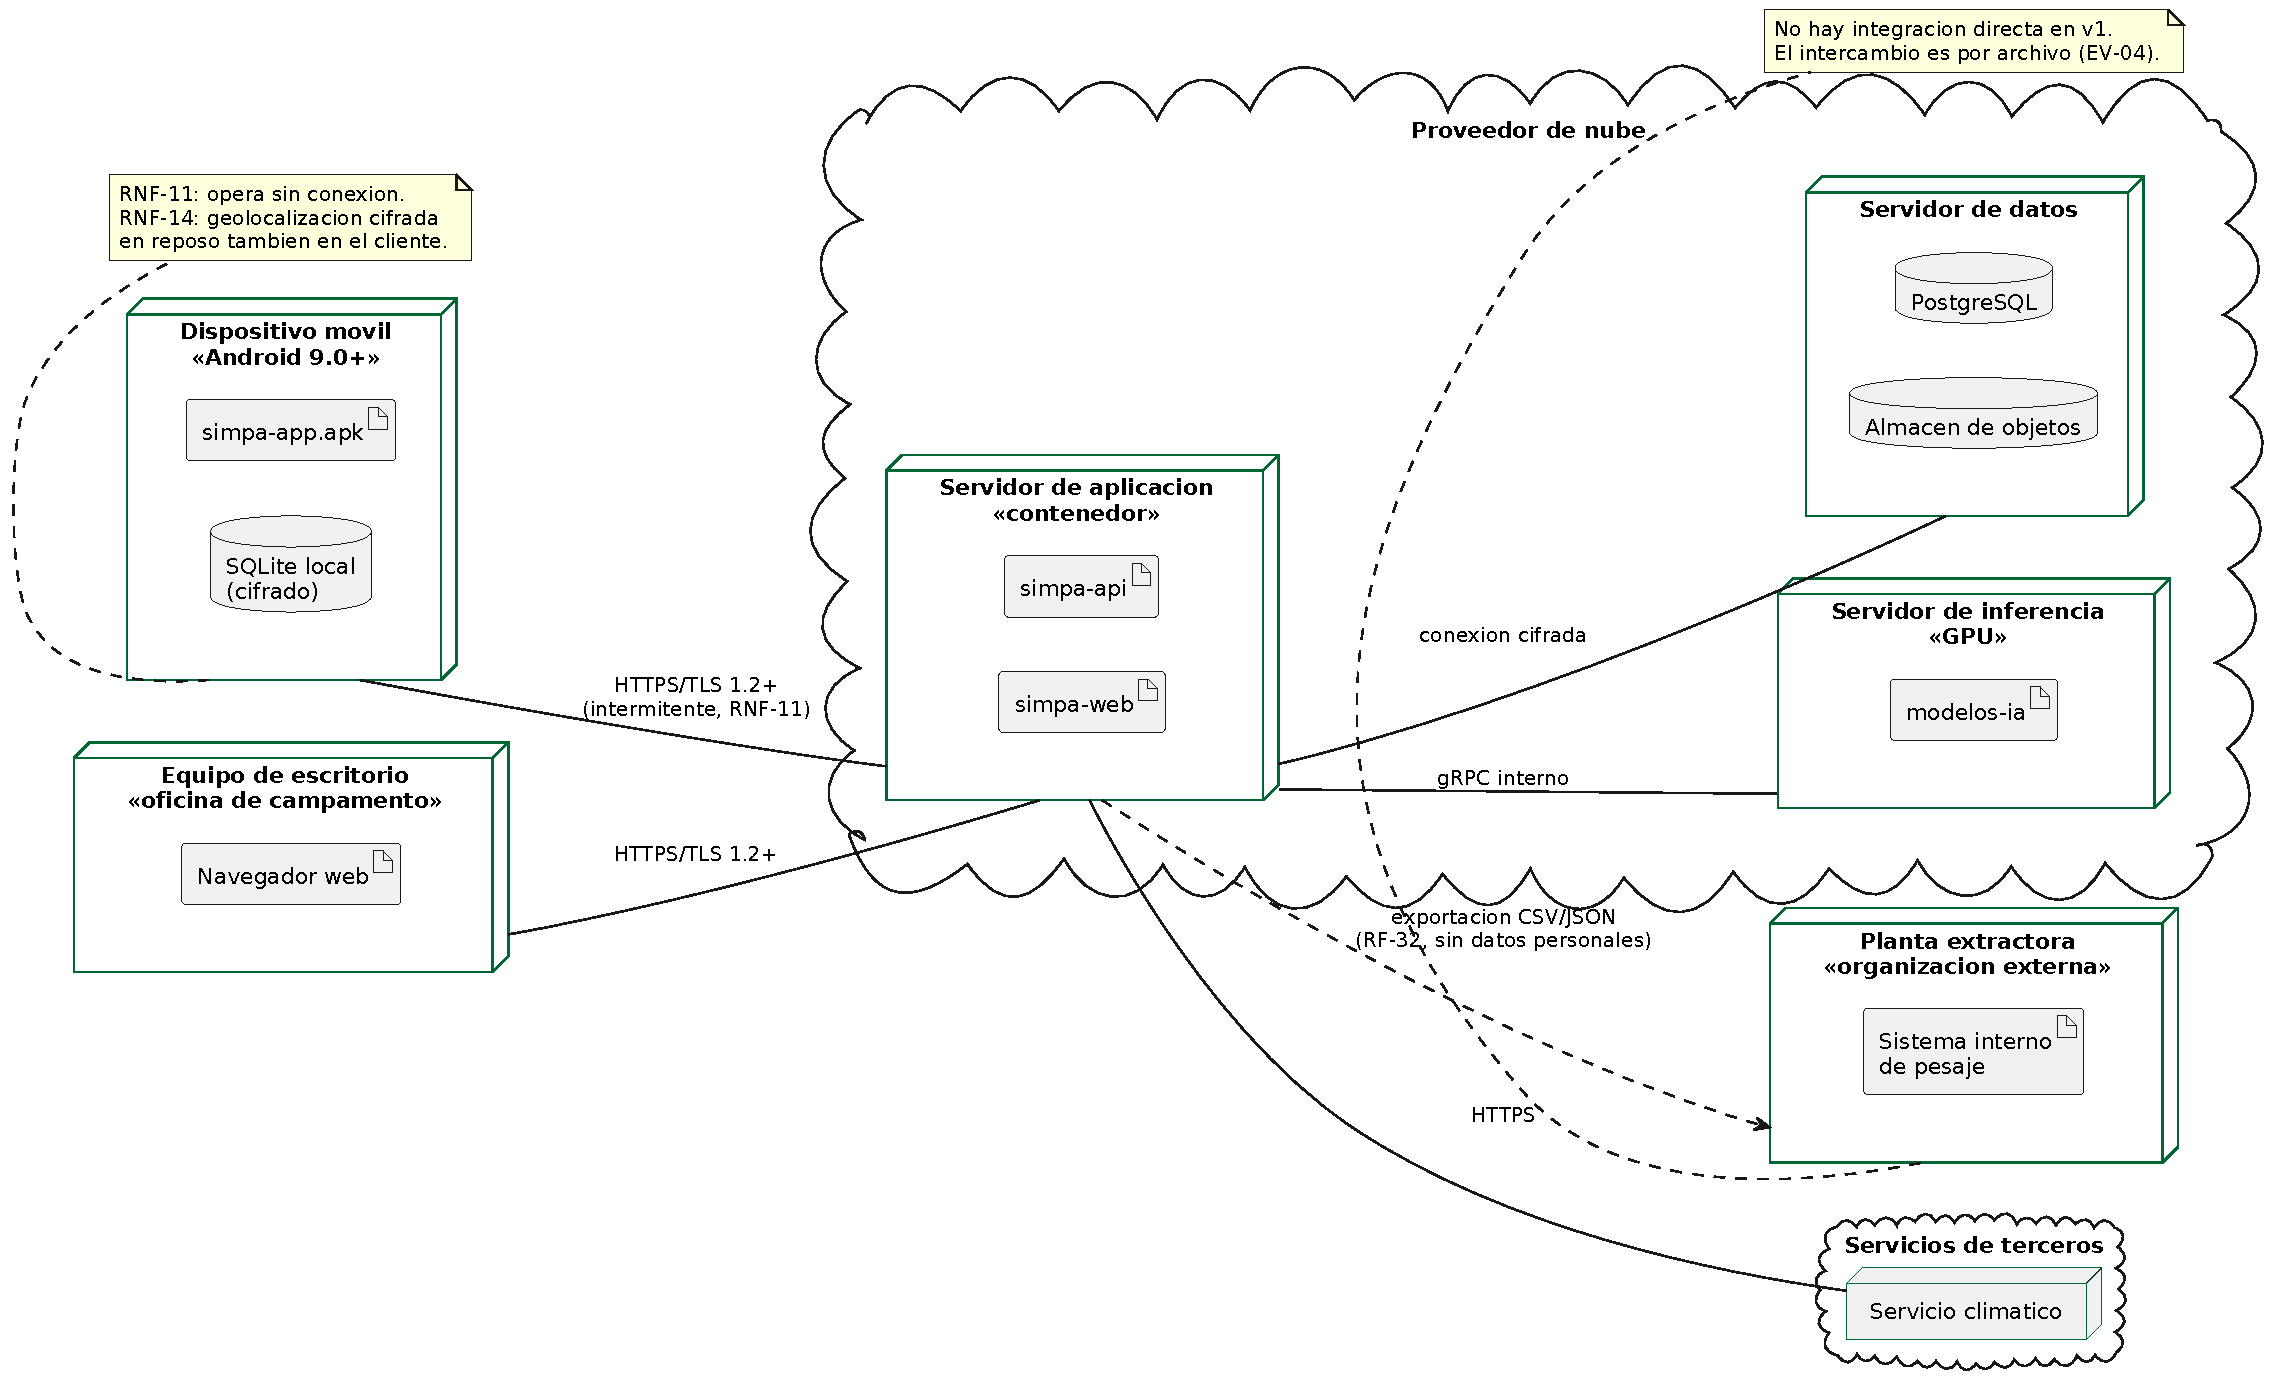
\includegraphics[width=1.0\textwidth]{img/despliegue}
\caption{Diagrama de despliegue del SIMPA.}
\label{fig:despliegue}
\end{figure}

\noindent
El enlace entre el dispositivo móvil y el servidor de aplicación se declara explícitamente como
\emph{intermitente}: el 74{,}2\% de las personas destinatarias no dispone de conectividad permanente
(\id{EV-12}). La planta extractora se representa como nodo externo sin integración directa; el
intercambio en la versión v1 se realiza por archivo, conforme a \id{RF-32}.

% ---------------------------------------------------------------------
\subsection{Cobertura del modelado}

\begin{longtable}{|L{4.6cm}|C{2.2cm}|C{2.2cm}|L{5.0cm}|}
\hline
\rowcolor{grisclaro}\textbf{Artefacto} & \textbf{Exigido} & \textbf{Entregado} & \textbf{Observación} \\
\hline
\endhead
Diagrama de casos de uso general & 1 & 1 & 8 actores, 18 casos de uso \\ \hline
Casos de uso detallados & 10 & 10 & Todos los \emph{Must}; $\geq 2$ flujos alternativos y $\geq 1$ excepción cada uno \\ \hline
Diagrama de clases refinado & 1 & 1 & 25 clases con atributos y operaciones \\ \hline
Diagramas de secuencia & CU \emph{Must} & 3 & CU-01, CU-03, CU-06 \\ \hline
Diagramas de actividad & Flujos principales & 1 & Ciclo semanal completo \\ \hline
Diagramas de estados & Entidades no triviales & 2 & Racimo y Alerta \\ \hline
Diagrama de componentes & 1 & 1 & --- \\ \hline
Diagrama de despliegue & 1 & 1 & --- \\ \hline
\caption{Cobertura del modelado UML frente a lo exigido en la §3.4 de la guía}
\end{longtable}

%  Requiere las imagenes en img/ generadas desde 03_Modelado/Diagramas_UML/
% =====================================================================

\newpage
\section{Modelado del sistema con UML}

El modelado emplea UML 2.5. Conforme a la §3.4 de la guía de la Entrega 3, se presentan ocho
diagramas: casos de uso general, especificación textual de diez casos de uso, clases refinado con
atributos y operaciones, tres diagramas de secuencia para los casos de uso \emph{Must}, actividad,
estados, componentes y despliegue. Todos se elaboraron en PlantUML y se entregan por triplicado
(fuente \id{.puml}, PNG a 300 dpi y SVG) en \id{03\_Modelado/Diagramas\_UML/}.

% ---------------------------------------------------------------------
\subsection{Diagrama general de casos de uso}

El diagrama presenta ocho actores y dieciocho casos de uso. Los actores primarios corresponden a los
seis perfiles de usuario de la §2.3; los actores secundarios son el servicio de análisis de IA y el
receptor GPS del dispositivo.

\begin{figure}[!htbp]
\centering
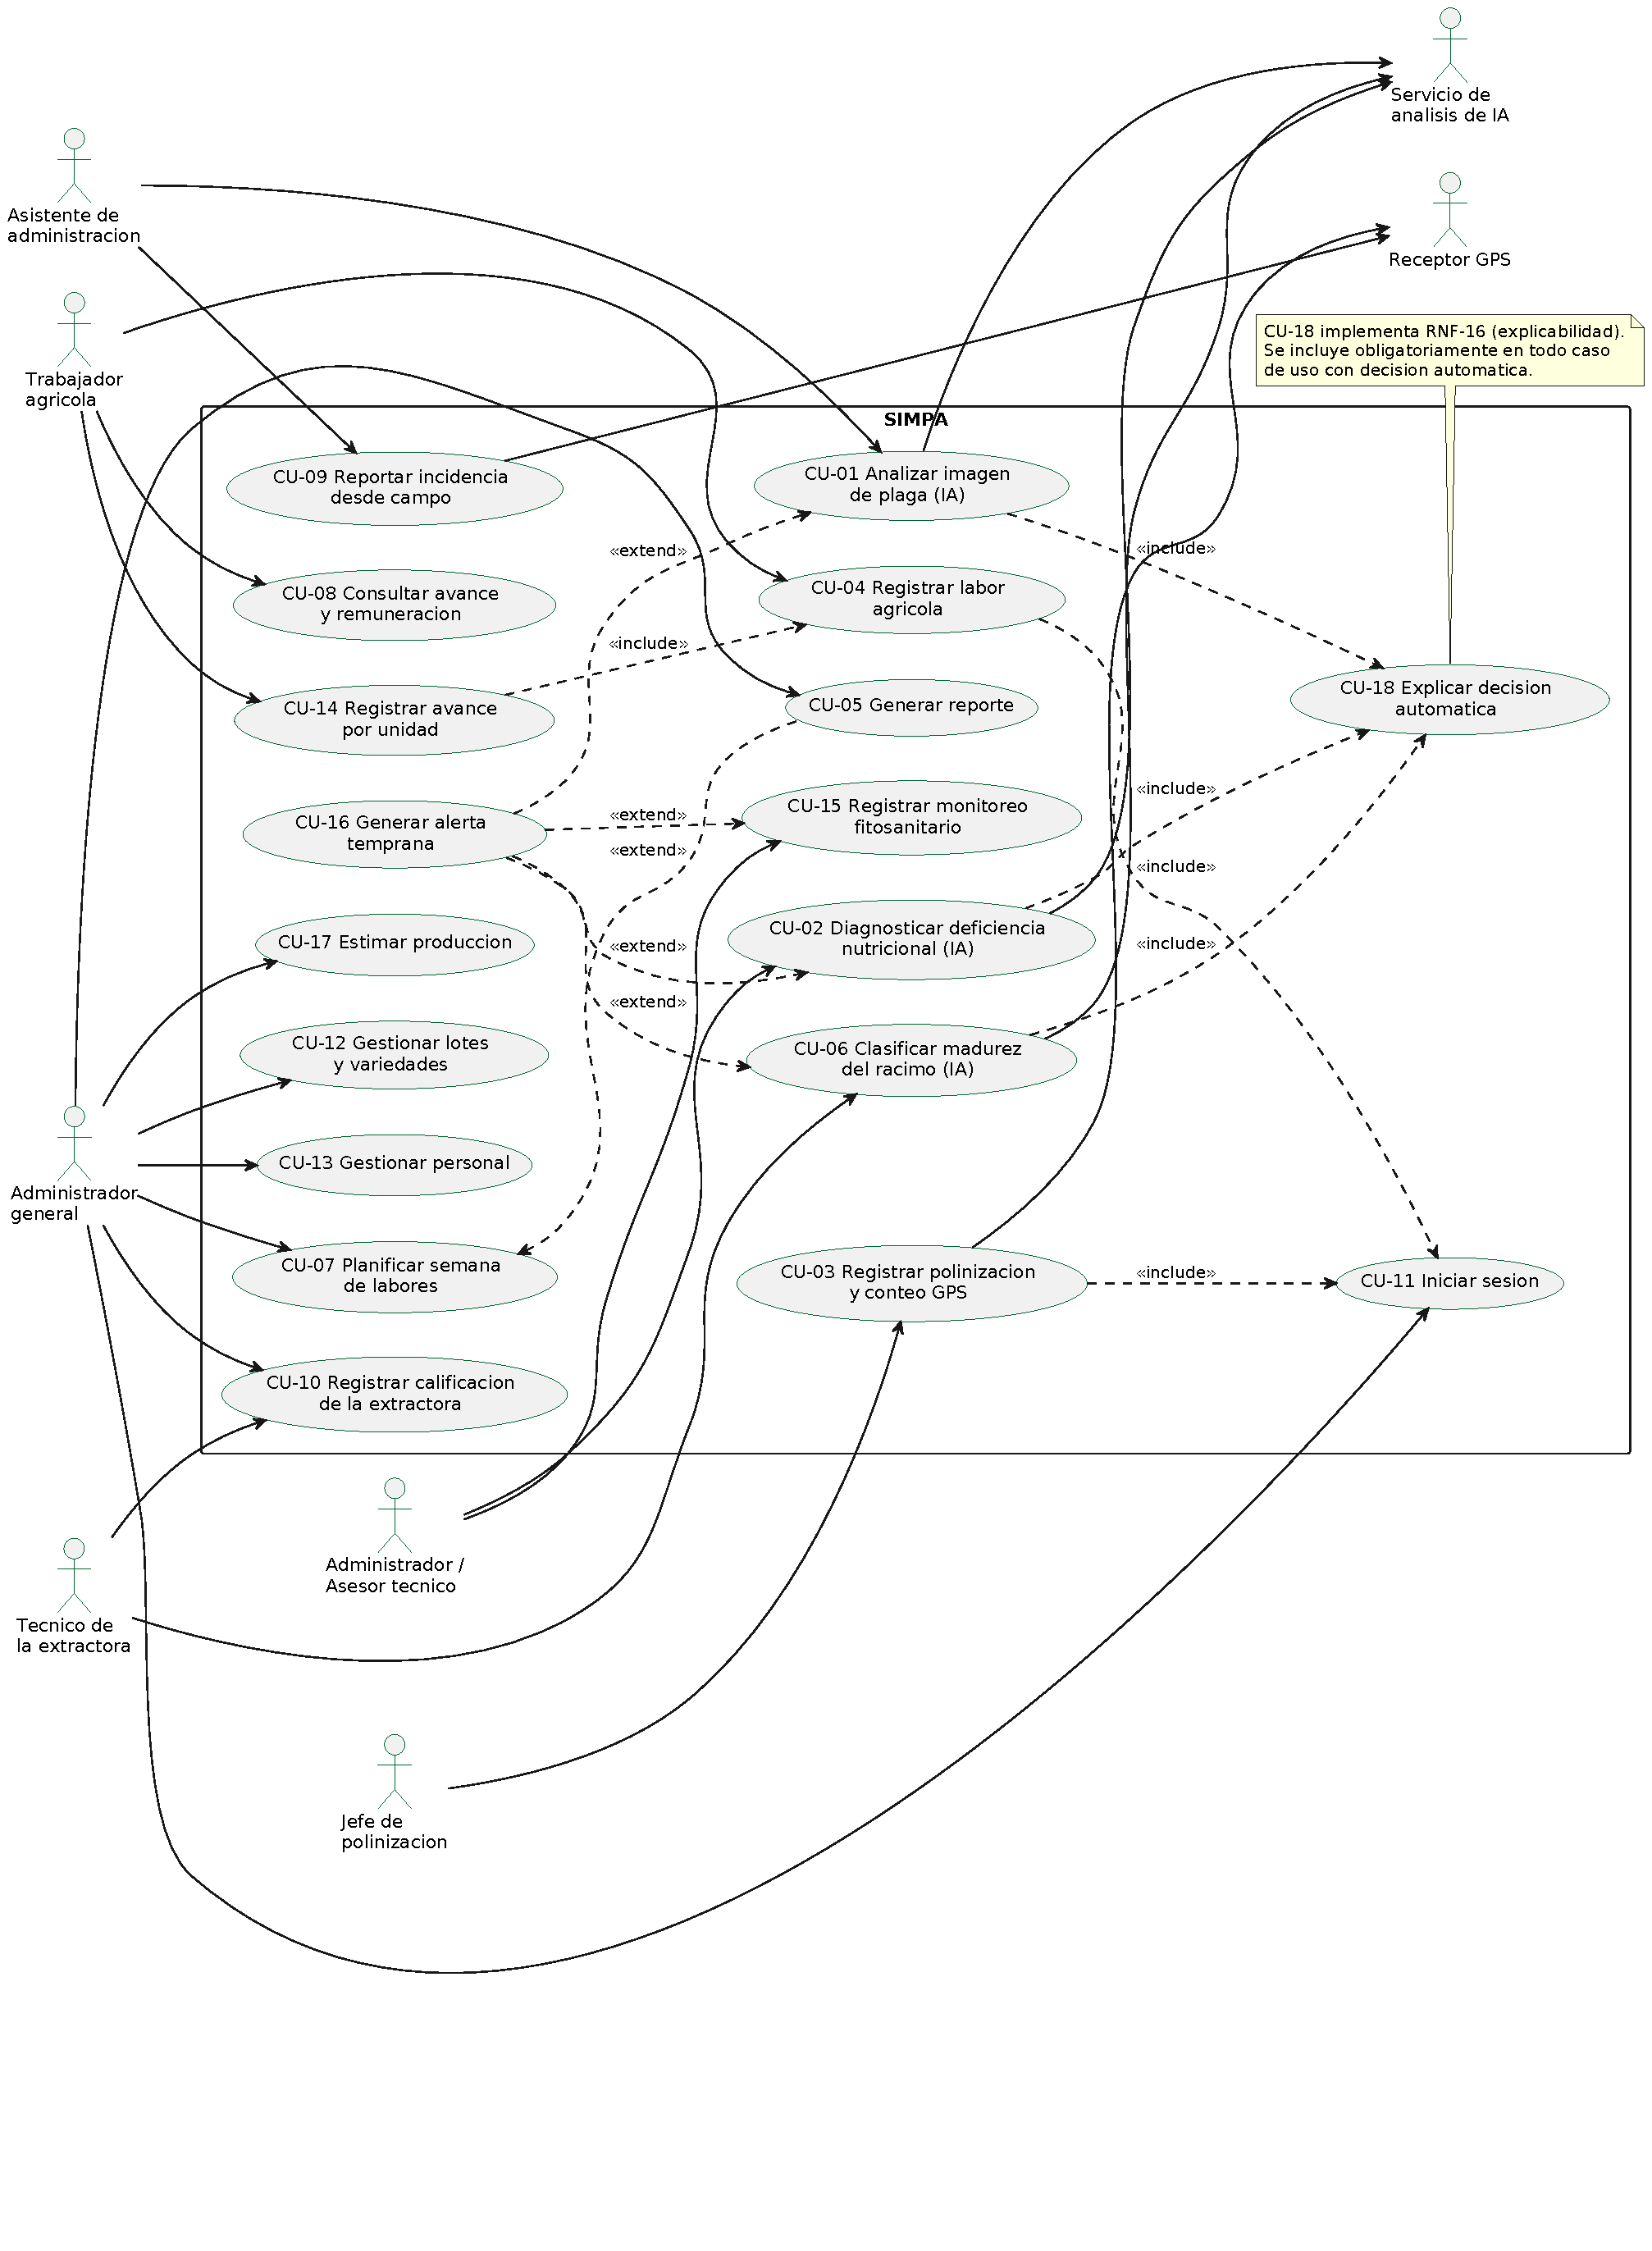
\includegraphics[width=0.91\textwidth]{img/casos_uso_general}
\caption{Diagrama general de casos de uso del SIMPA, con los ocho actores y el límite del sistema.}
\label{fig:cu_general}
\end{figure}

\noindent\textbf{Relaciones de inclusión y extensión.} \id{CU-14} incluye a \id{CU-04}, dado que el
registro de avance presupone una labor registrada. \id{CU-04} y \id{CU-03} incluyen a \id{CU-11},
por requerir sesión autenticada. Los tres casos de uso con decisión automática ---\id{CU-01},
\id{CU-02} y \id{CU-06}--- incluyen obligatoriamente a \id{CU-18}, que materializa el requisito de
explicabilidad \id{RNF-16}: no existe decisión automática sin explicación asociada. \id{CU-16}
extiende a los casos de diagnóstico y de monitoreo, puesto que la alerta se genera únicamente si el
resultado es positivo.

% ---------------------------------------------------------------------
\subsection{Especificación textual de los casos de uso}

Se especifican diez casos de uso, correspondientes a la totalidad de los requisitos funcionales de
prioridad \emph{Must}. Cada especificación incluye actores, precondiciones, postcondiciones, flujo
principal, al menos un flujo alternativo y al menos una excepción.

% --- CU-01
\begin{longtable}{|L{3.4cm}|L{12.0cm}|}
\hline
\rowcolor{grisclaro}\multicolumn{2}{|l|}{\textbf{CU-01 --- Analizar imagen para detectar plaga o enfermedad}}\\
\hline
\textbf{Requisitos} & \id{RF-07}, \id{RF-09}, \id{RF-12}, \id{RNF-16} \\ \hline
\textbf{Actores} & Primario: técnico fitosanitario / asistente de administración. Secundario: servicio de análisis de IA. \\ \hline
\textbf{Precondición} & Persona usuaria autenticada; lote seleccionado; cámara disponible. \\ \hline
\textbf{Postcondición} & El diagnóstico y su explicación quedan registrados y asociados al lote y a la fecha. \\ \hline
\textbf{Flujo principal} & 1. La persona usuaria selecciona el lote y la opción \emph{Analizar imagen}. \newline 2. Captura la fotografía de la palma o de la hoja. \newline 3. El sistema valida la calidad de la imagen. \newline 4. El sistema envía la imagen al servicio de IA con los parámetros de la variedad del lote. \newline 5. El servicio devuelve la clase de afectación, el nivel de confianza y el rasgo visual determinante. \newline 6. El sistema genera la explicación conforme a \id{RNF-16}. \newline 7. El sistema muestra el resultado, la explicación y la recomendación de control, y registra el diagnóstico. \\ \hline
\textbf{Flujo alternativo A} & \emph{Sin conectividad.} En el paso 4 el sistema almacena la imagen localmente y encola el análisis; al restablecerse la conexión lo ejecuta y notifica el resultado (\id{RNF-11}). \\ \hline
\textbf{Flujo alternativo B} & \emph{Confianza insuficiente.} Si el nivel de confianza es inferior al umbral configurado, el sistema no emite clasificación: informa que el resultado no es concluyente y sugiere repetir la captura o consultar a la asesoría técnica. \\ \hline
\textbf{Excepción E1} & Imagen de calidad insuficiente: el sistema solicita repetir la captura indicando el defecto detectado. \\ \hline
\textbf{Excepción E2} & Servicio de IA no disponible: el análisis queda en estado pendiente y la persona usuaria es notificada. \\ \hline
\textbf{Extensión} & Si el resultado es positivo, se ejecuta \id{CU-16} (generar alerta temprana). \\ \hline
\caption{CU-01 --- Analizar imagen para detectar plaga o enfermedad}
\end{longtable}

% --- CU-02
\begin{longtable}{|L{3.4cm}|L{12.0cm}|}
\hline
\rowcolor{grisclaro}\multicolumn{2}{|l|}{\textbf{CU-02 --- Diagnosticar deficiencia nutricional por imagen}}\\
\hline
\textbf{Requisitos} & \id{RF-08}, \id{RF-11}, \id{RNF-16} \\ \hline
\textbf{Actores} & Primario: administrador / asesor técnico. Secundario: servicio de análisis de IA. \\ \hline
\textbf{Precondición} & Persona usuaria autenticada; lote seleccionado con variedad asignada. \\ \hline
\textbf{Postcondición} & El diagnóstico nutricional y su recomendación quedan registrados en el historial del lote. \\ \hline
\textbf{Flujo principal} & 1. La persona usuaria selecciona \emph{Diagnóstico nutricional} y el lote. \newline 2. Captura la fotografía de la hoja. \newline 3. El sistema valida la imagen y la envía al servicio de IA. \newline 4. El servicio estima el elemento deficiente. \newline 5. El sistema genera una explicación de tipo causal, indicando qué signo foliar sustenta la estimación. \newline 6. El sistema muestra la deficiencia, la recomendación de fertilización y la explicación, y registra el diagnóstico. \\ \hline
\textbf{Flujo alternativo A} & La persona usuaria adjunta una imagen existente de la galería en lugar de capturarla. \\ \hline
\textbf{Flujo alternativo B} & \emph{Contraste con análisis de laboratorio.} Si el lote tiene un análisis de suelo o foliar registrado (\id{RF-11}), el sistema contrasta la estimación con los valores medidos y señala la discrepancia si la hubiere. \\ \hline
\textbf{Excepción E1} & Imagen no válida: el sistema solicita repetir la captura. \\ \hline
\textbf{Excepción E2} & Lote sin variedad asignada: el sistema advierte que la estimación puede no ser aplicable y solicita completar el dato. \\ \hline
\textbf{Extensión} & Si la deficiencia estimada es severa, se ejecuta \id{CU-16}. \\ \hline
\caption{CU-02 --- Diagnosticar deficiencia nutricional por imagen}
\end{longtable}

% --- CU-03
\begin{longtable}{|L{3.4cm}|L{12.0cm}|}
\hline
\rowcolor{grisclaro}\multicolumn{2}{|l|}{\textbf{CU-03 --- Registrar polinización y conteo georreferenciado}}\\
\hline
\textbf{Requisitos} & \id{RF-13}, \id{RF-14}, \id{RNF-05}, \id{RNF-12}, \id{RL-03} \\ \hline
\textbf{Actores} & Primario: polinizador. Secundario: receptor GPS. \\ \hline
\textbf{Precondición} & Lote en etapa de polinización; sesión iniciada; consentimiento de geolocalización vigente. \\ \hline
\textbf{Postcondición} & La polinización y el conteo diario quedan registrados por persona, lote y fecha, sin ingreso manual planta por planta. \\ \hline
\textbf{Flujo principal} & 1. El polinizador inicia la jornada en el lote. \newline 2. El sistema verifica la vigencia del consentimiento de geolocalización. \newline 3. El sistema activa el rastreo con período de muestreo de 30 s. \newline 4. Durante la jornada, el sistema almacena las marcaciones georreferenciadas. \newline 5. El polinizador registra el estado de la antesis y la verificación visual. \newline 6. Al cierre, el sistema calcula el número de flores polinizadas a partir de las marcaciones. \newline 7. El sistema almacena el registro y muestra el total a la persona trabajadora. \\ \hline
\textbf{Flujo alternativo A} & \emph{Consentimiento revocado.} Si el consentimiento no está vigente, el sistema no activa el rastreo y habilita el registro manual del número de flores, sin penalización para la persona trabajadora (\id{RL-03}). \\ \hline
\textbf{Flujo alternativo B} & \emph{Sin conectividad.} Las marcaciones se almacenan localmente y se sincronizan al reconectar (\id{RNF-11}). \\ \hline
\textbf{Excepción E1} & Precisión GPS superior a 10 m: el sistema conserva el dato marcándolo como de precisión degradada y advierte a la persona usuaria, sin descartar la jornada (\id{RNF-12}). \\ \hline
\textbf{Excepción E2} & Pérdida total de señal GPS durante la jornada: el sistema conserva el tramo registrado y solicita completar el conteo de forma manual para el tramo faltante. \\ \hline
\caption{CU-03 --- Registrar polinización y conteo georreferenciado}
\end{longtable}

% --- CU-04
\begin{longtable}{|L{3.4cm}|L{12.0cm}|}
\hline
\rowcolor{grisclaro}\multicolumn{2}{|l|}{\textbf{CU-04 --- Registrar labor agrícola}}\\
\hline
\textbf{Requisitos} & \id{RF-04}, \id{RF-28}, \id{RF-35} \\ \hline
\textbf{Actores} & Primario: trabajador agrícola. Alternativo: jefe de campo (registro delegado). \\ \hline
\textbf{Precondición} & Lote y persona trabajadora registrados; persona usuaria autenticada. \\ \hline
\textbf{Postcondición} & La labor y su avance quedan en el historial del lote y computan para el cumplimiento del plan semanal. \\ \hline
\textbf{Flujo principal} & 1. La persona usuaria selecciona el lote y el tipo de labor. \newline 2. Ingresa la cantidad ejecutada en la unidad correspondiente. \newline 3. El sistema valida que la unidad corresponda al tipo de labor. \newline 4. El sistema registra la labor asociada al lote, la fecha y la persona responsable. \newline 5. El sistema actualiza el avance acumulado del período y el cumplimiento de la meta semanal. \\ \hline
\textbf{Flujo alternativo A} & \emph{Registro delegado.} Si la persona trabajadora no dispone de dispositivo propio, el jefe de campo registra el avance en su nombre; el sistema conserva en bitácora la identidad de quien efectuó el registro (\id{RF-35}, \id{RD-10}). \\ \hline
\textbf{Flujo alternativo B} & \emph{Sin conectividad.} La labor se almacena localmente y se sincroniza al reconectar. \\ \hline
\textbf{Excepción E1} & Datos incompletos: el sistema impide guardar y señala los campos faltantes. \\ \hline
\textbf{Excepción E2} & Unidad incompatible con el tipo de labor: el sistema rechaza el registro e indica la unidad esperada. \\ \hline
\caption{CU-04 --- Registrar labor agrícola}
\end{longtable}

% --- CU-05
\begin{longtable}{|L{3.4cm}|L{12.0cm}|}
\hline
\rowcolor{grisclaro}\multicolumn{2}{|l|}{\textbf{CU-05 --- Generar reporte}}\\
\hline
\textbf{Requisitos} & \id{RF-19}, \id{RF-26} \\ \hline
\textbf{Actores} & Primario: administrador general. \\ \hline
\textbf{Precondición} & Existen registros en el período seleccionado. \\ \hline
\textbf{Postcondición} & El reporte queda disponible para consulta o exportación. \\ \hline
\textbf{Flujo principal} & 1. La persona administradora selecciona el tipo de reporte y el período. \newline 2. El sistema consolida labores, avance, producción y alertas del período. \newline 3. El sistema genera y presenta el reporte. \newline 4. La persona administradora lo consulta o lo exporta a PDF o a hoja de cálculo. \\ \hline
\textbf{Flujo alternativo A} & Filtrado por lote, por equipo o por persona trabajadora. \\ \hline
\textbf{Flujo alternativo B} & \emph{Reporte de cumplimiento semanal.} El sistema contrasta el plan de la semana con lo ejecutado y destaca las metas no alcanzadas y su remanente. \\ \hline
\textbf{Excepción E1} & Sin registros en el período: el sistema informa la ausencia de datos y propone un período alternativo con información disponible. \\ \hline
\caption{CU-05 --- Generar reporte}
\end{longtable}

% --- CU-06
\begin{longtable}{|L{3.4cm}|L{12.0cm}|}
\hline
\rowcolor{grisclaro}\multicolumn{2}{|l|}{\textbf{CU-06 --- Clasificar la madurez del racimo}}\\
\hline
\textbf{Requisitos} & \id{RF-21}, \id{RF-22}, \id{RD-07}, \id{RD-08}, \id{RNF-01}, \id{RNF-16} \\ \hline
\textbf{Actores} & Primario: cosechador / técnico de la extractora. Secundario: servicio de análisis de IA. \\ \hline
\textbf{Precondición} & Lote con variedad asignada; persona usuaria autenticada. \\ \hline
\textbf{Postcondición} & La clasificación queda asociada al racimo, al lote y a la fecha, y actualiza el porcentaje estimado de fruta verde del lote. \\ \hline
\textbf{Flujo principal} & 1. La persona usuaria selecciona el lote y la opción \emph{Clasificar racimo}. \newline 2. El sistema recupera el umbral de desprendimiento de la variedad del lote. \newline 3. La persona usuaria captura la fotografía de la parte basal del racimo. \newline 4. El servicio de IA cuenta los frutos desprendidos, sin emplear el color como criterio (\id{RD-07}). \newline 5. El sistema compara el conteo con el umbral de la variedad y determina el estado. \newline 6. El sistema genera una explicación por contraste, indicando el conteo obtenido y el umbral aplicable. \newline 7. El sistema registra la clasificación y actualiza el porcentaje de fruta verde del lote. \\ \hline
\textbf{Flujo alternativo A} & \emph{Verificación previa al despacho.} La persona usuaria solicita el porcentaje estimado de fruta verde del lote; si alcanza o supera el umbral de penalización, el sistema emite alerta preventiva y desaconseja el despacho (\id{RF-22}). \\ \hline
\textbf{Flujo alternativo B} & \emph{Sobremadurez.} Si el conteo excede ampliamente el umbral, el sistema clasifica el racimo como sobremaduro y advierte sobre el incremento de acidez. \\ \hline
\textbf{Excepción E1} & Lote sin variedad asignada: el sistema no clasifica y solicita completar el dato, dado que el umbral depende de la variedad. \\ \hline
\textbf{Excepción E2} & Parte basal no visible en la imagen: el sistema solicita repetir la captura indicando el encuadre requerido. \\ \hline
\caption{CU-06 --- Clasificar la madurez del racimo}
\end{longtable}

% --- CU-07
\begin{longtable}{|L{3.4cm}|L{12.0cm}|}
\hline
\rowcolor{grisclaro}\multicolumn{2}{|l|}{\textbf{CU-07 --- Planificar la semana de labores}}\\
\hline
\textbf{Requisitos} & \id{RF-26}, \id{RF-27}, \id{RF-34}, \id{RF-37} a \id{RF-39} \\ \hline
\textbf{Actores} & Primario: administrador general. \\ \hline
\textbf{Precondición} & Lotes y tipos de labor registrados. \\ \hline
\textbf{Postcondición} & El plan de la semana queda publicado y disponible para el seguimiento diario. \\ \hline
\textbf{Flujo principal} & 1. La persona administradora crea el plan de la semana. \newline 2. Para cada lote, define las labores previstas con su meta y unidad. \newline 3. El sistema incorpora automáticamente los remanentes arrastrados de la semana anterior. \newline 4. La persona administradora registra los insumos requeridos. \newline 5. El sistema publica el plan y lo hace visible al jefe de campo. \\ \hline
\textbf{Flujo alternativo A} & \emph{Cierre de semana.} Al cierre, el sistema calcula el cumplimiento de cada meta; si es parcial, genera el remanente como labor pendiente de la semana siguiente, vinculada a la de origen (\id{RF-27}). \\ \hline
\textbf{Flujo alternativo B} & Ajuste del plan durante la semana en curso, conservando la versión previa en bitácora. \\ \hline
\textbf{Flujo alternativo C} & \emph{Liquidación y aprobación.} Al cierre, el sistema genera la liquidación que contrasta cantidad presupuestada, cantidad ejecutada, tarifa y valor por grupo de labor, totaliza el gasto presupuestado frente al real, e incorpora las labores no presupuestadas en su grupo diferenciado (\id{RF-37}, \id{RF-38}). La persona administradora aprueba la liquidación y el período queda cerrado (\id{RF-39}). \\ \hline
\textbf{Excepción E1} & Meta expresada en unidad incompatible con el tipo de labor: el sistema rechaza la meta e indica la unidad esperada. \\ \hline
\textbf{Excepción E2} & Existe un plan publicado para la misma semana: el sistema advierte y solicita confirmación antes de sustituirlo. \\ \hline
\caption{CU-07 --- Planificar la semana de labores}
\end{longtable}

% --- CU-08
\begin{longtable}{|L{3.4cm}|L{12.0cm}|}
\hline
\rowcolor{grisclaro}\multicolumn{2}{|l|}{\textbf{CU-08 --- Consultar avance acumulado y remuneración estimada}}\\
\hline
\textbf{Requisitos} & \id{RF-29}, \id{RF-36}, \id{RL-04} \\ \hline
\textbf{Actores} & Primario: trabajador agrícola. \\ \hline
\textbf{Precondición} & Existen registros de avance de la persona trabajadora en el período. \\ \hline
\textbf{Postcondición} & Se presenta el consolidado del período, sin posibilidad de edición por parte de la persona trabajadora. \\ \hline
\textbf{Flujo principal} & 1. La persona trabajadora accede a \emph{Mi avance}. \newline 2. Selecciona el período (quincena en curso por defecto). \newline 3. El sistema agrega sus registros de avance por tipo de labor. \newline 4. El sistema obtiene del catálogo la tarifa vigente de cada tipo de labor a la fecha de cada registro y calcula la remuneración estimada correspondiente al trabajo por avance. \newline 5. El sistema presenta el desglose por labor y el total estimado. \\ \hline
\textbf{Flujo alternativo A} & \emph{Ejercicio del derecho de acceso.} La persona trabajadora solicita la exportación de sus datos personales; el sistema genera el archivo conforme al Art. 12 de la LOPDP (\id{RL-04}). \\ \hline
\textbf{Flujo alternativo B} & \emph{Discrepancia.} La persona trabajadora marca un registro como discrepante; el sistema notifica a la administración sin modificar el dato original, y la corrección se tramita mediante \id{RL-05}. \\ \hline
\textbf{Excepción E1} & Sin registros en el período: el sistema informa la ausencia de datos. \\ \hline
\textbf{Excepción E2} & La labor carece de tarifa vigente en el catálogo (\id{RF-36}) a la fecha del registro: el sistema muestra el avance en unidades, omite la estimación monetaria e indica que la tarifa no está vigente para esa fecha. \\ \hline
\caption{CU-08 --- Consultar avance acumulado y remuneración estimada}
\end{longtable}

% --- CU-09
\begin{longtable}{|L{3.4cm}|L{12.0cm}|}
\hline
\rowcolor{grisclaro}\multicolumn{2}{|l|}{\textbf{CU-09 --- Reportar incidencia desde el campo}}\\
\hline
\textbf{Requisitos} & \id{RF-30}, \id{RF-31}, \id{RF-12} \\ \hline
\textbf{Actores} & Primario: asistente de administración / trabajador agrícola. Secundario: receptor GPS. \\ \hline
\textbf{Precondición} & Persona usuaria autenticada; cámara y GPS disponibles. \\ \hline
\textbf{Postcondición} & La incidencia queda registrada con fotografía y coordenadas, e incorporada a la lista de pendientes de verificación. \\ \hline
\textbf{Flujo principal} & 1. La persona usuaria selecciona \emph{Reportar incidencia}. \newline 2. Captura la fotografía de la afectación. \newline 3. El sistema obtiene las coordenadas del punto. \newline 4. La persona usuaria selecciona el lote y describe la afectación. \newline 5. El sistema registra la incidencia georreferenciada. \newline 6. El sistema la incorpora a la lista de pendientes de la persona supervisora. \\ \hline
\textbf{Flujo alternativo A} & \emph{Análisis asistido.} La persona usuaria solicita el análisis de la fotografía; se ejecuta \id{CU-01} y el diagnóstico se asocia a la incidencia. \\ \hline
\textbf{Flujo alternativo B} & \emph{Verificación en visita.} La persona supervisora recorre su lista de pendientes, ubica la incidencia por sus coordenadas y la marca como verificada o descartada. \\ \hline
\textbf{Excepción E1} & GPS no disponible: el sistema registra la incidencia solicitando la selección manual del lote y la marca como de ubicación aproximada. \\ \hline
\textbf{Excepción E2} & Sin conectividad: la incidencia se encola y se sincroniza al reconectar, conservando el instante original de captura. \\ \hline
\caption{CU-09 --- Reportar incidencia desde el campo}
\end{longtable}

% --- CU-10
\begin{longtable}{|L{3.4cm}|L{12.0cm}|}
\hline
\rowcolor{grisclaro}\multicolumn{2}{|l|}{\textbf{CU-10 --- Registrar la calificación de la planta extractora}}\\
\hline
\textbf{Requisitos} & \id{RF-23}, \id{RF-24}, \id{RF-25}, \id{RF-33} \\ \hline
\textbf{Actores} & Primario: administrador general. \\ \hline
\textbf{Precondición} & Existe un despacho registrado con su fecha de corte. \\ \hline
\textbf{Postcondición} & La calificación queda asociada al lote de origen y disponible para el análisis de trazabilidad. \\ \hline
\textbf{Flujo principal} & 1. La persona administradora selecciona el despacho. \newline 2. Ingresa los datos del ticket de pesaje: peso bruto, tara y neto. \newline 3. Ingresa la calificación de calidad: tamaño del fruto, porcentaje de fruta verde, sobremadura, malformación y pedúnculo largo. \newline 4. El sistema calcula el intervalo entre el corte y la entrega. \newline 5. El sistema registra la calificación y la asocia al lote de origen. \\ \hline
\textbf{Flujo alternativo A} & \emph{Análisis de trazabilidad.} Ante una calificación desfavorable, la persona administradora consulta la cadena lote $\rightarrow$ fecha de corte $\rightarrow$ cuadrilla, y contrasta con las labores del período para distinguir si el origen está en la cosecha o en el manejo del cultivo (\id{RF-24}). \\ \hline
\textbf{Flujo alternativo B} & \emph{Ausencia de guía de remisión.} Si el despacho se registra sin número de guía, el sistema advierte antes del cierre (\id{RF-33}). \\ \hline
\textbf{Excepción E1} & El intervalo entre corte y entrega supera el valor recomendado para la variedad: el sistema registra la advertencia junto al despacho (\id{RF-25}). \\ \hline
\textbf{Excepción E2} & La suma de pesos es inconsistente (neto distinto de bruto menos tara): el sistema rechaza el registro e indica la inconsistencia. \\ \hline
\caption{CU-10 --- Registrar la calificación de la planta extractora}
\end{longtable}

% ---------------------------------------------------------------------
\subsection{Diagrama de clases refinado}

El modelo del dominio comprende veinticinco clases con atributos y operaciones. Incorpora tres
jerarquías de herencia (\id{Persona}--\id{Usuario} y la especialización de \id{Diagnostico} en sus
tres variantes), cuatro relaciones de composición y asociaciones con multiplicidad explícita. No
corresponde a un diseño de base de datos, sino al modelo conceptual del dominio del problema.

\begin{figure}[!htbp]
\centering
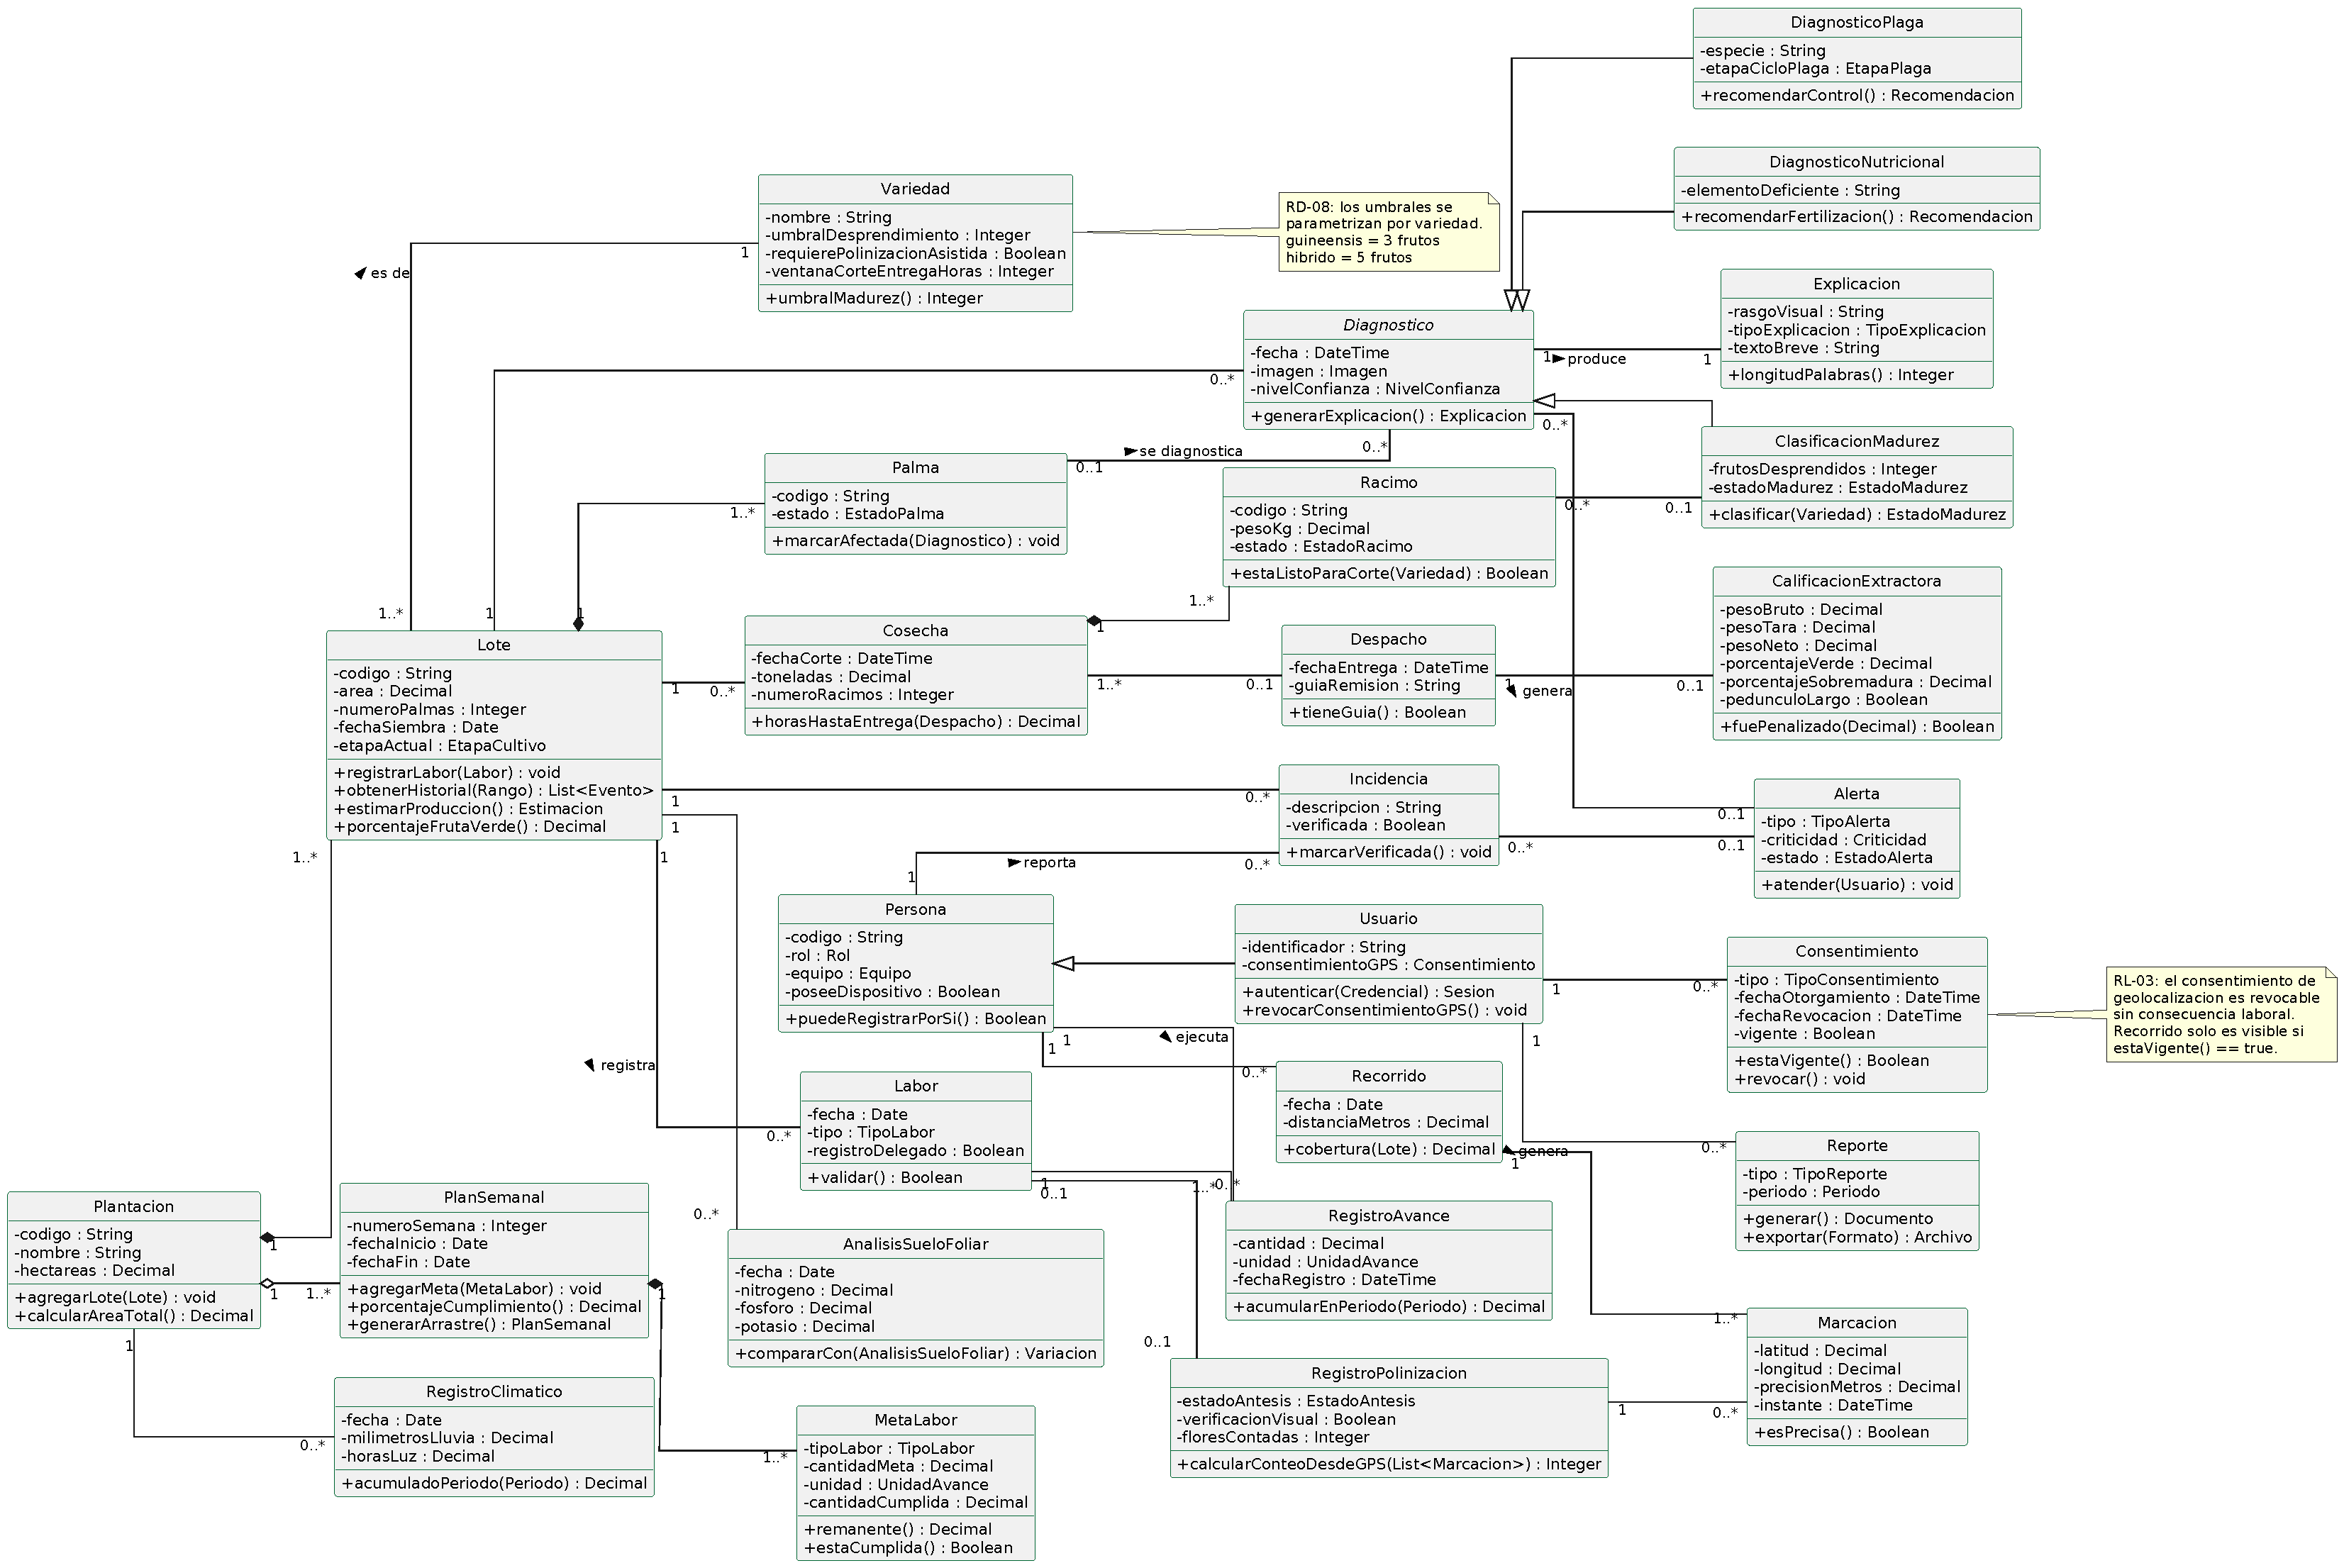
\includegraphics[width=1.0\textwidth]{img/clases_refinado}
\caption{Diagrama de clases refinado del SIMPA, con atributos y operaciones.}
\label{fig:clases}
\end{figure}

\noindent\textbf{Decisiones de modelado relevantes.} La clase \id{Consentimiento} se modela como
entidad de primer orden y no como atributo booleano de \id{Usuario}, porque el Art. 7 de la LOPDP
exige que el consentimiento sea específico por finalidad y revocable, lo que obliga a conservar su
historia. La clase \id{Variedad} concentra los umbrales de decisión ---desprendimiento, ventana
corte-entrega y necesidad de polinización asistida--- en lugar de fijarlos en la lógica de los
módulos de IA, conforme a \id{RD-08}. La clase \id{Explicacion} se asocia de forma obligatoria a
\id{Diagnostico} con multiplicidad 1:1, de modo que el modelo impide estructuralmente la existencia
de una decisión automática sin explicación (\id{RNF-16}). La clase \id{RegistroAvance} se separa de
\id{Labor} porque una labor puede acumular avances de varias personas y días, patrón observado en
los documentos de planificación semanal (\id{EV-11}).

% ---------------------------------------------------------------------
\subsection{Diagramas de secuencia}

Se presentan los diagramas de secuencia de los tres casos de uso \emph{Must} de mayor complejidad
de interacción.

\begin{figure}[!htbp]
\centering
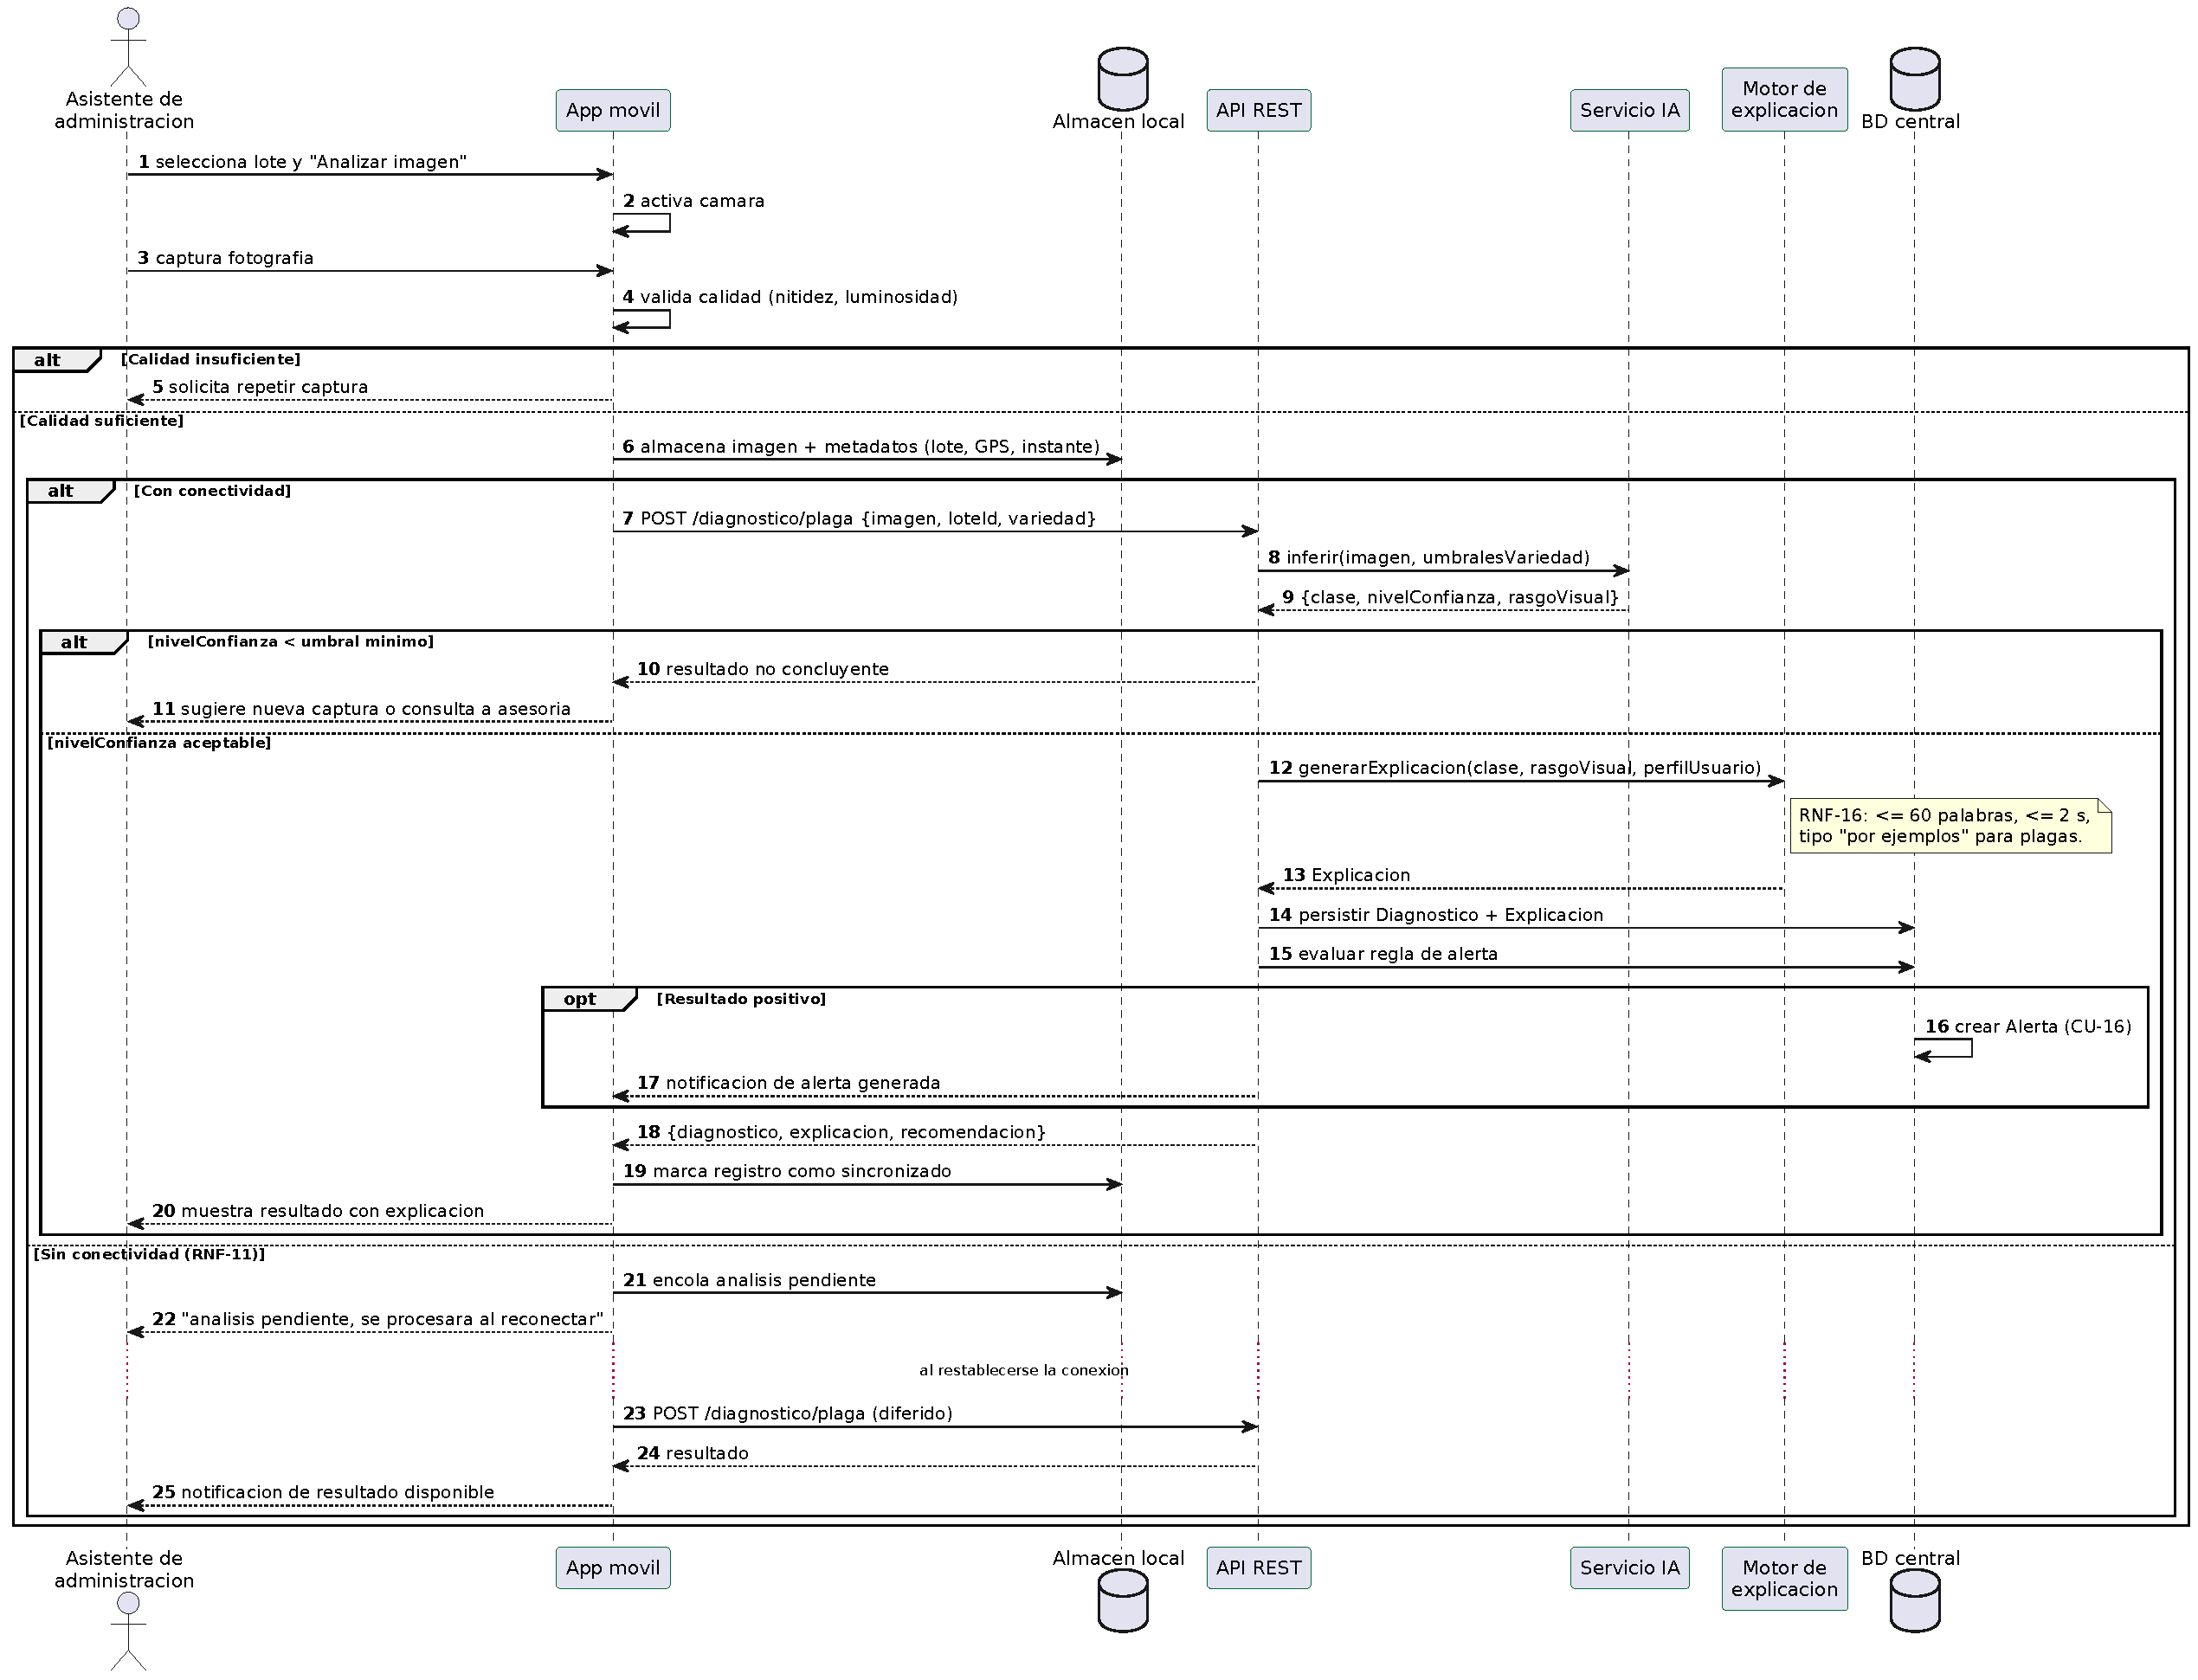
\includegraphics[width=1.0\textwidth]{img/secuencia_CU01}
\caption{Diagrama de secuencia del CU-01: análisis de imagen para detección de plaga, con las ramas de baja confianza y de operación sin conectividad.}
\label{fig:seq01}
\end{figure}

\begin{figure}[!htbp]
\centering
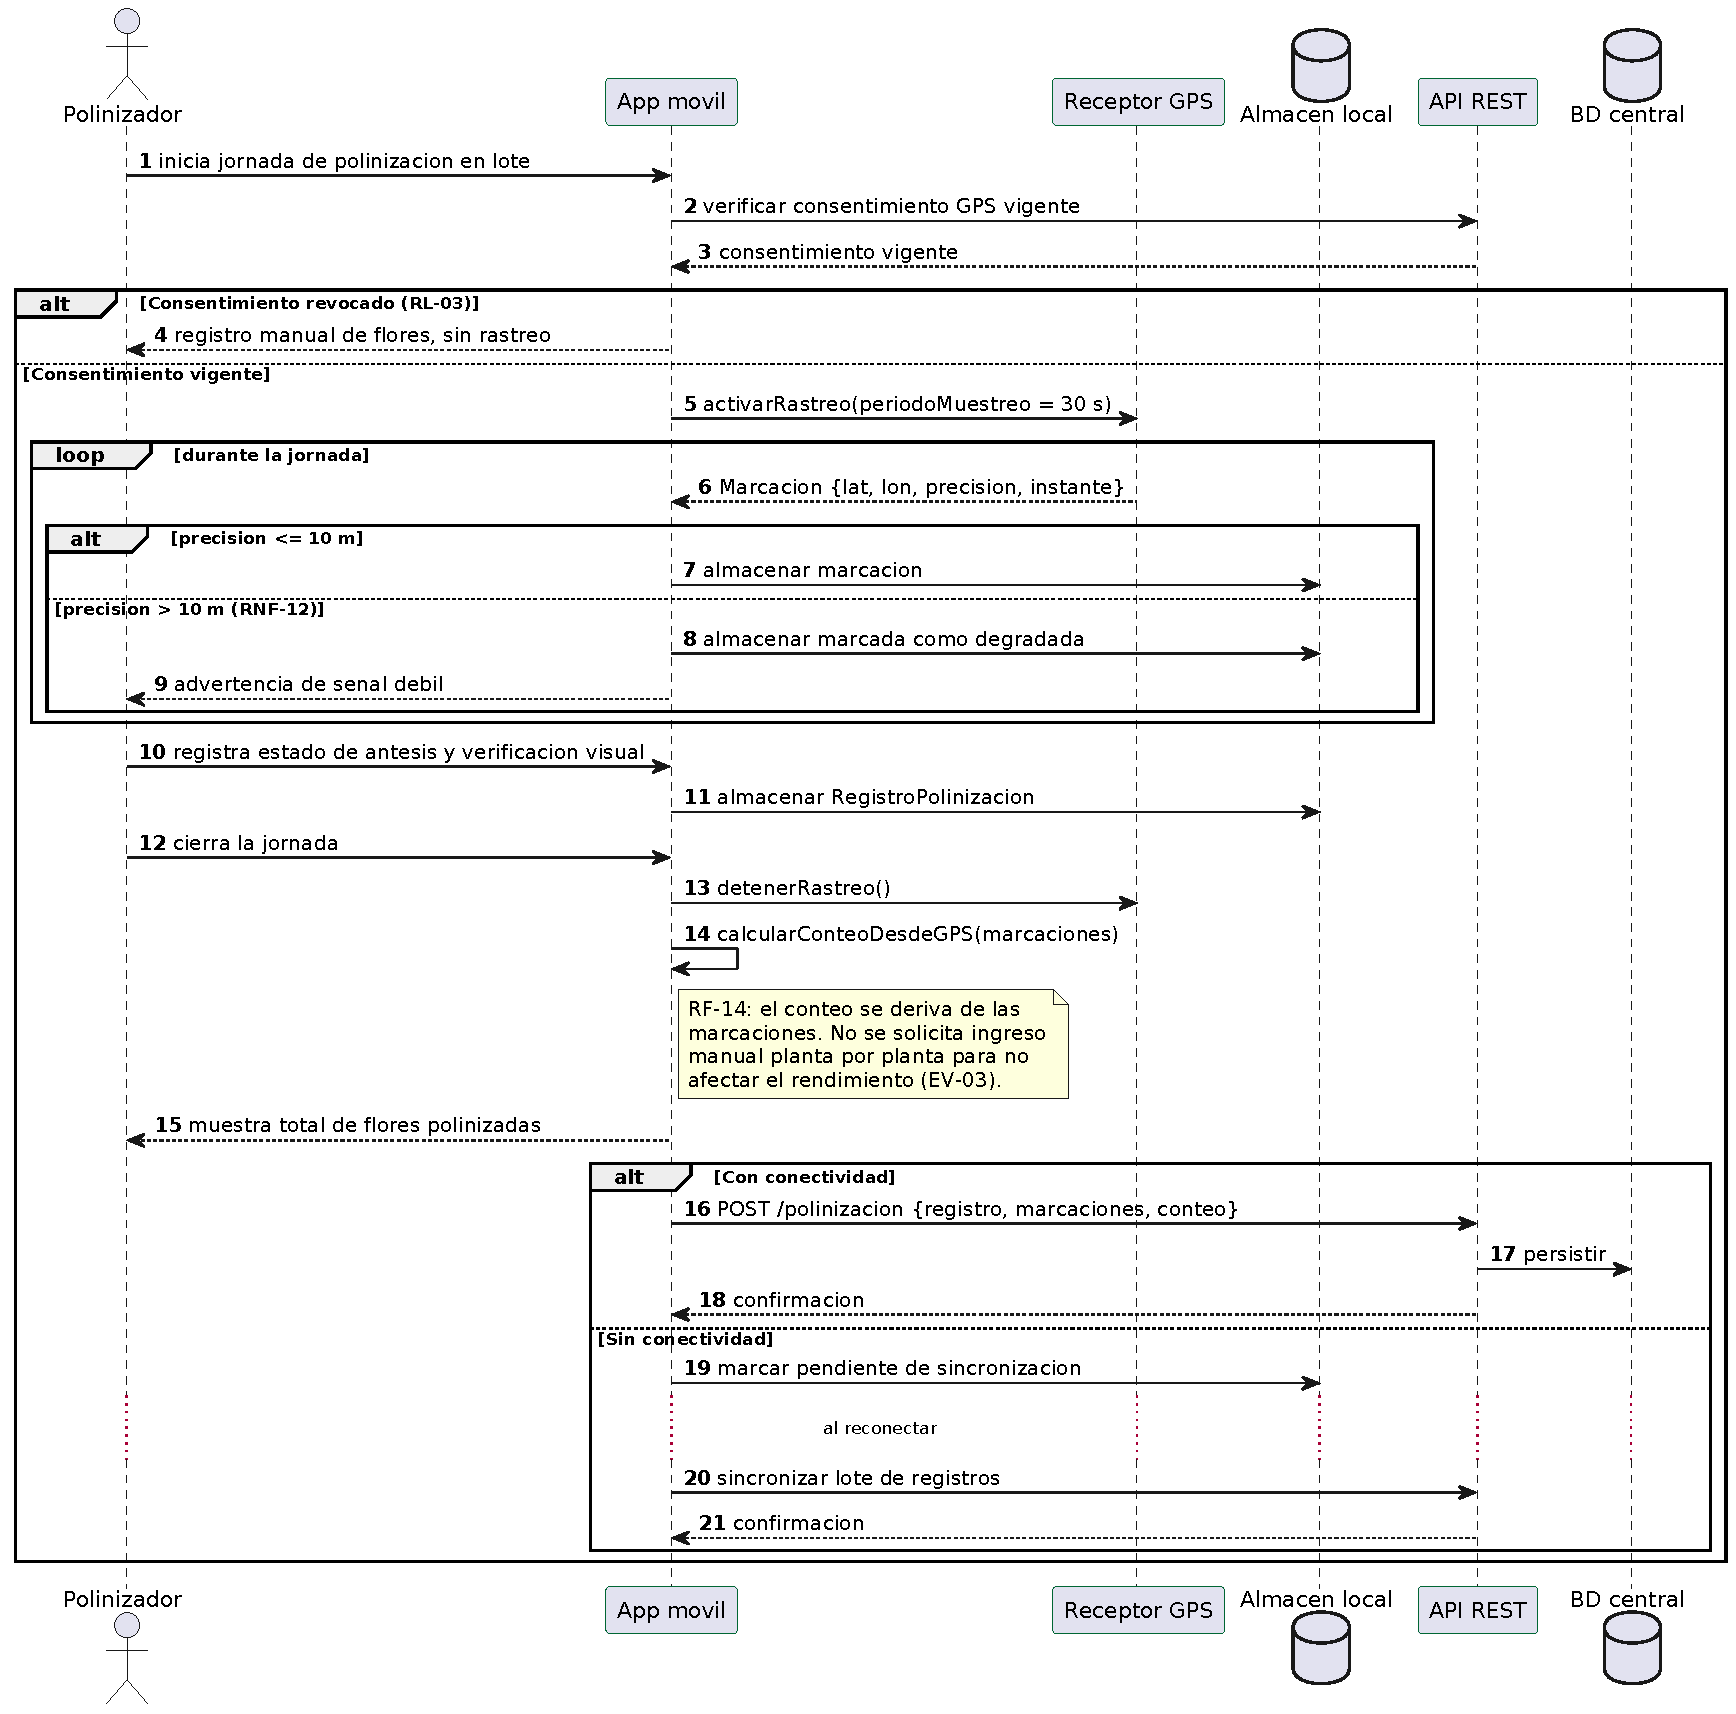
\includegraphics[width=1.0\textwidth]{img/secuencia_CU03}
\caption{Diagrama de secuencia del CU-03: registro de polinización y conteo georreferenciado, con verificación de consentimiento y manejo de precisión degradada.}
\label{fig:seq03}
\end{figure}

\begin{figure}[!htbp]
\centering
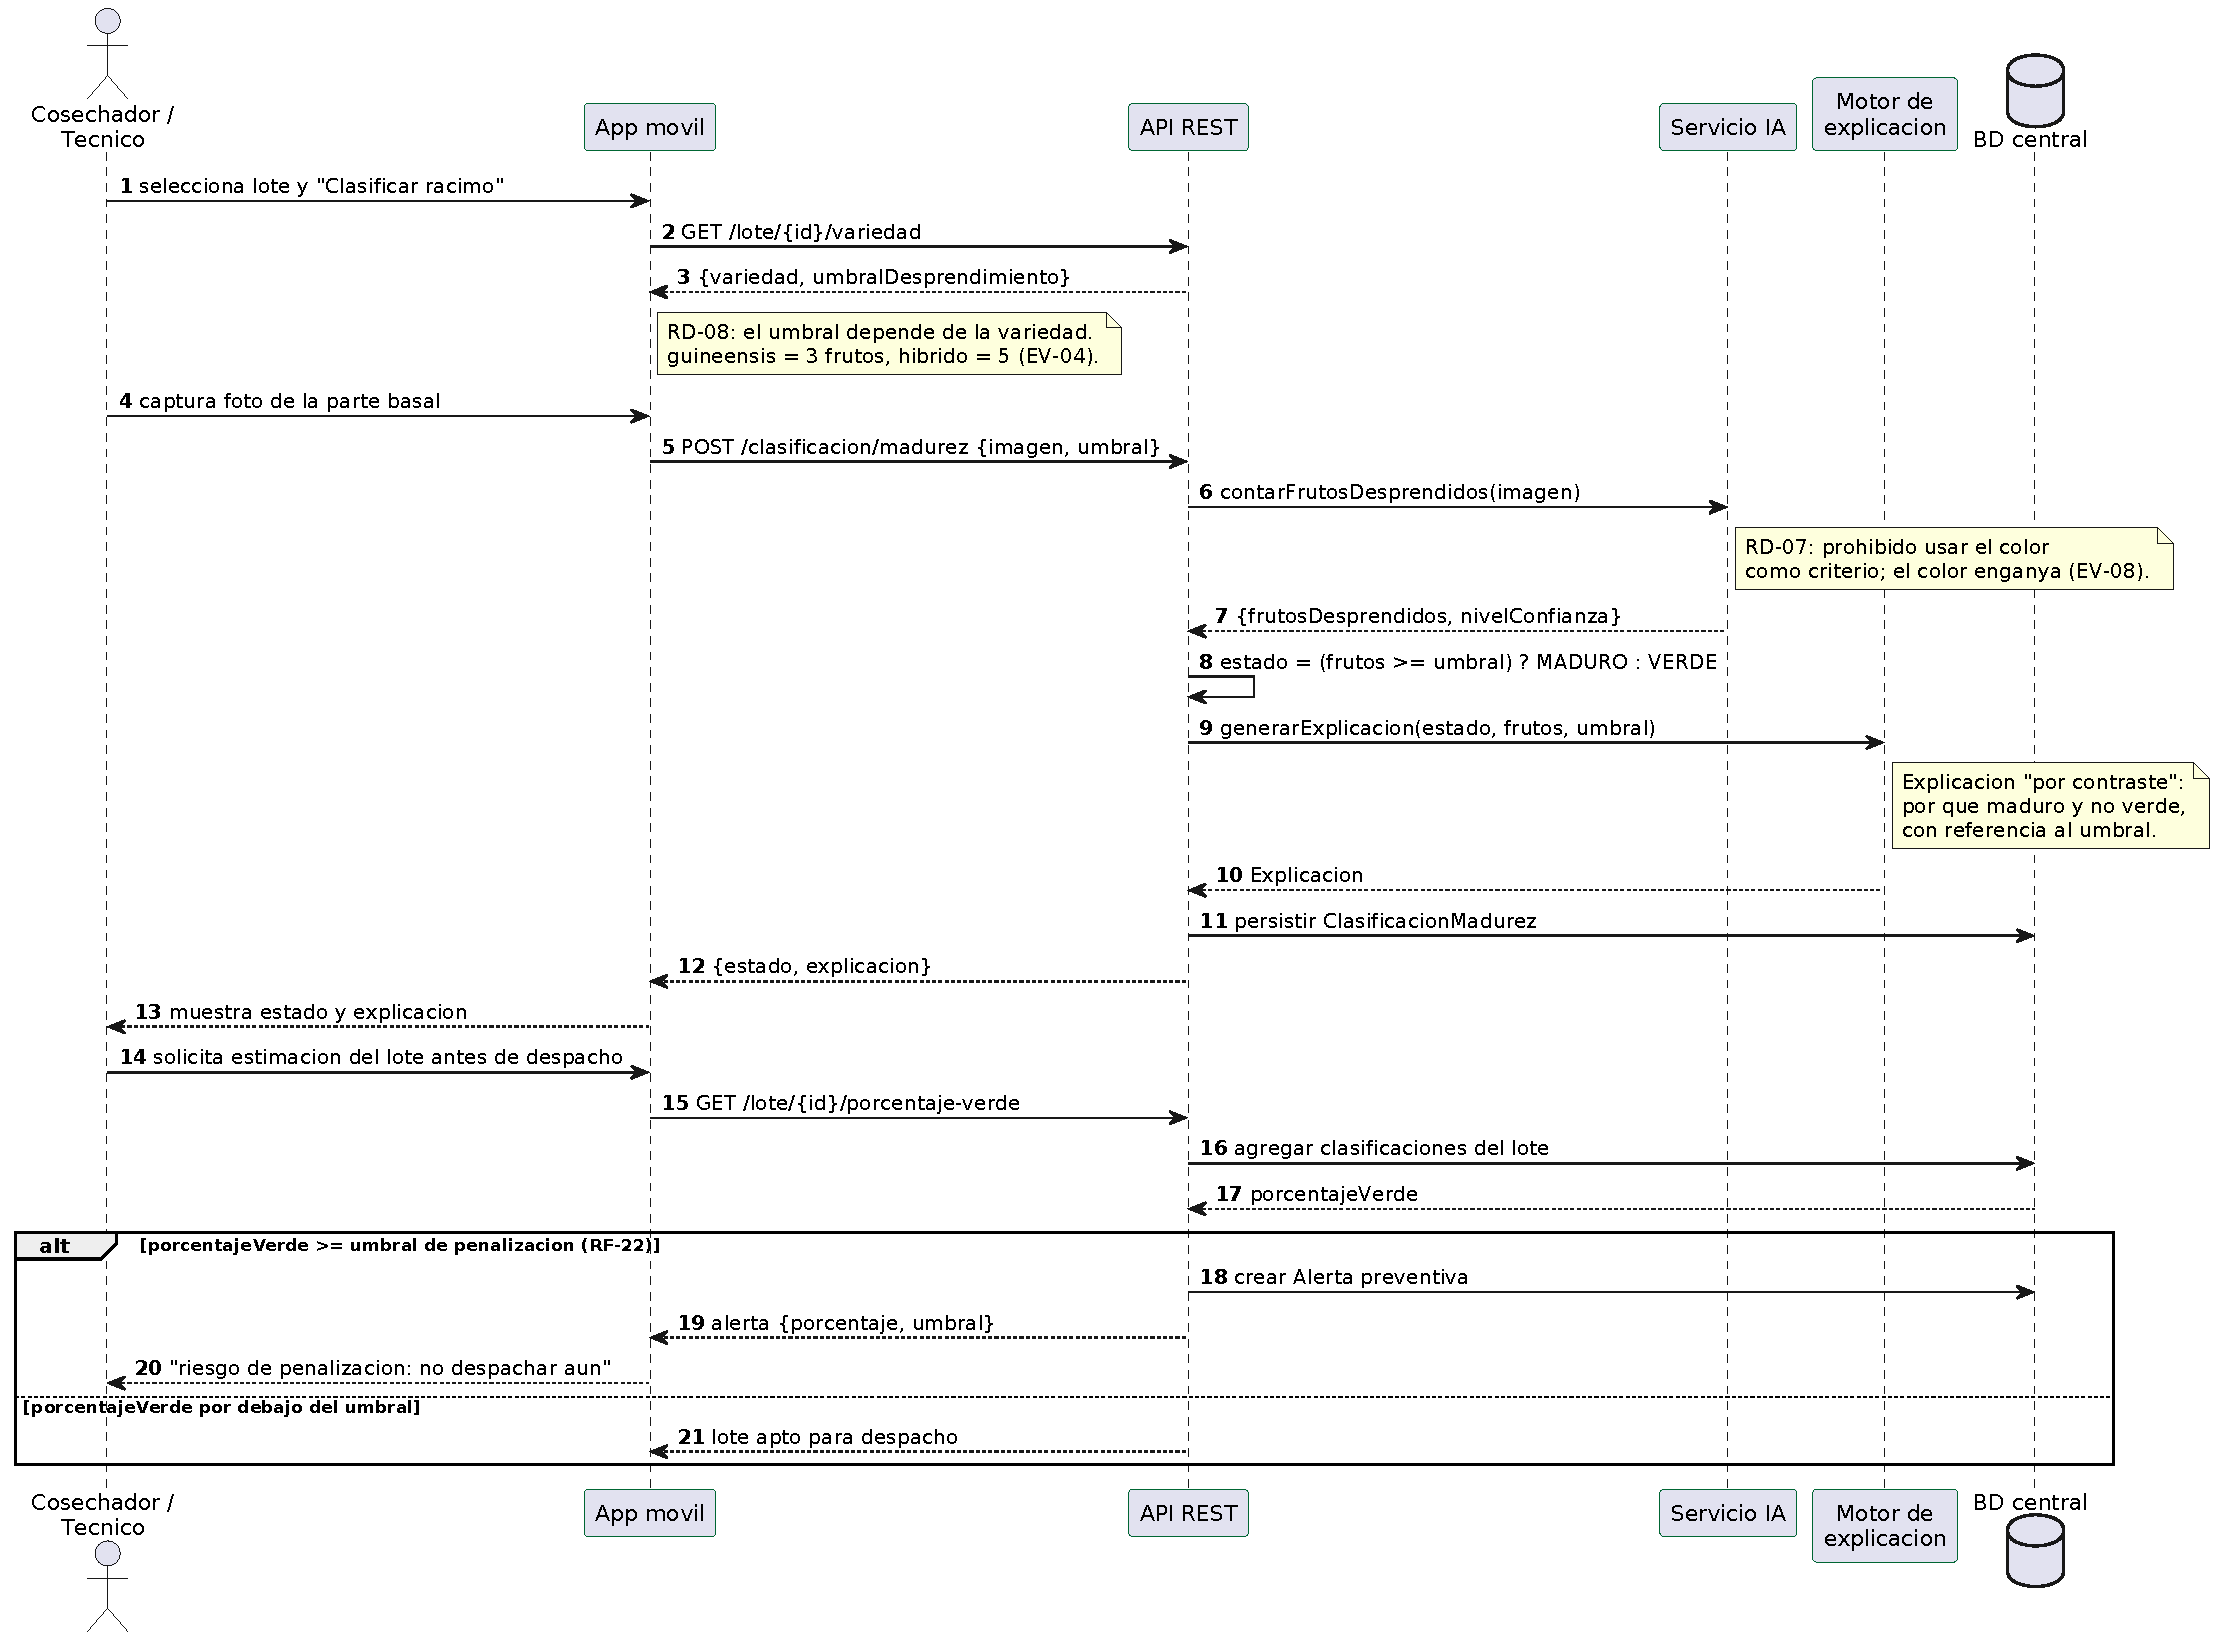
\includegraphics[width=1.0\textwidth]{img/secuencia_CU06}
\caption{Diagrama de secuencia del CU-06: clasificación de madurez del racimo y alerta preventiva de porcentaje de fruta verde.}
\label{fig:seq06}
\end{figure}

% ---------------------------------------------------------------------
\subsection{Diagrama de actividad}

El diagrama modela el ciclo semanal completo de planificación y ejecución, que constituye el proceso
central de la organización según los documentos operativos (\id{EV-11}). Incorpora la bifurcación
por disponibilidad de dispositivo (\id{RF-35}), la bifurcación por conectividad (\id{RNF-11}) y el
mecanismo de arrastre de labor incompleta (\id{RF-27}).

\begin{figure}[!htbp]
\centering
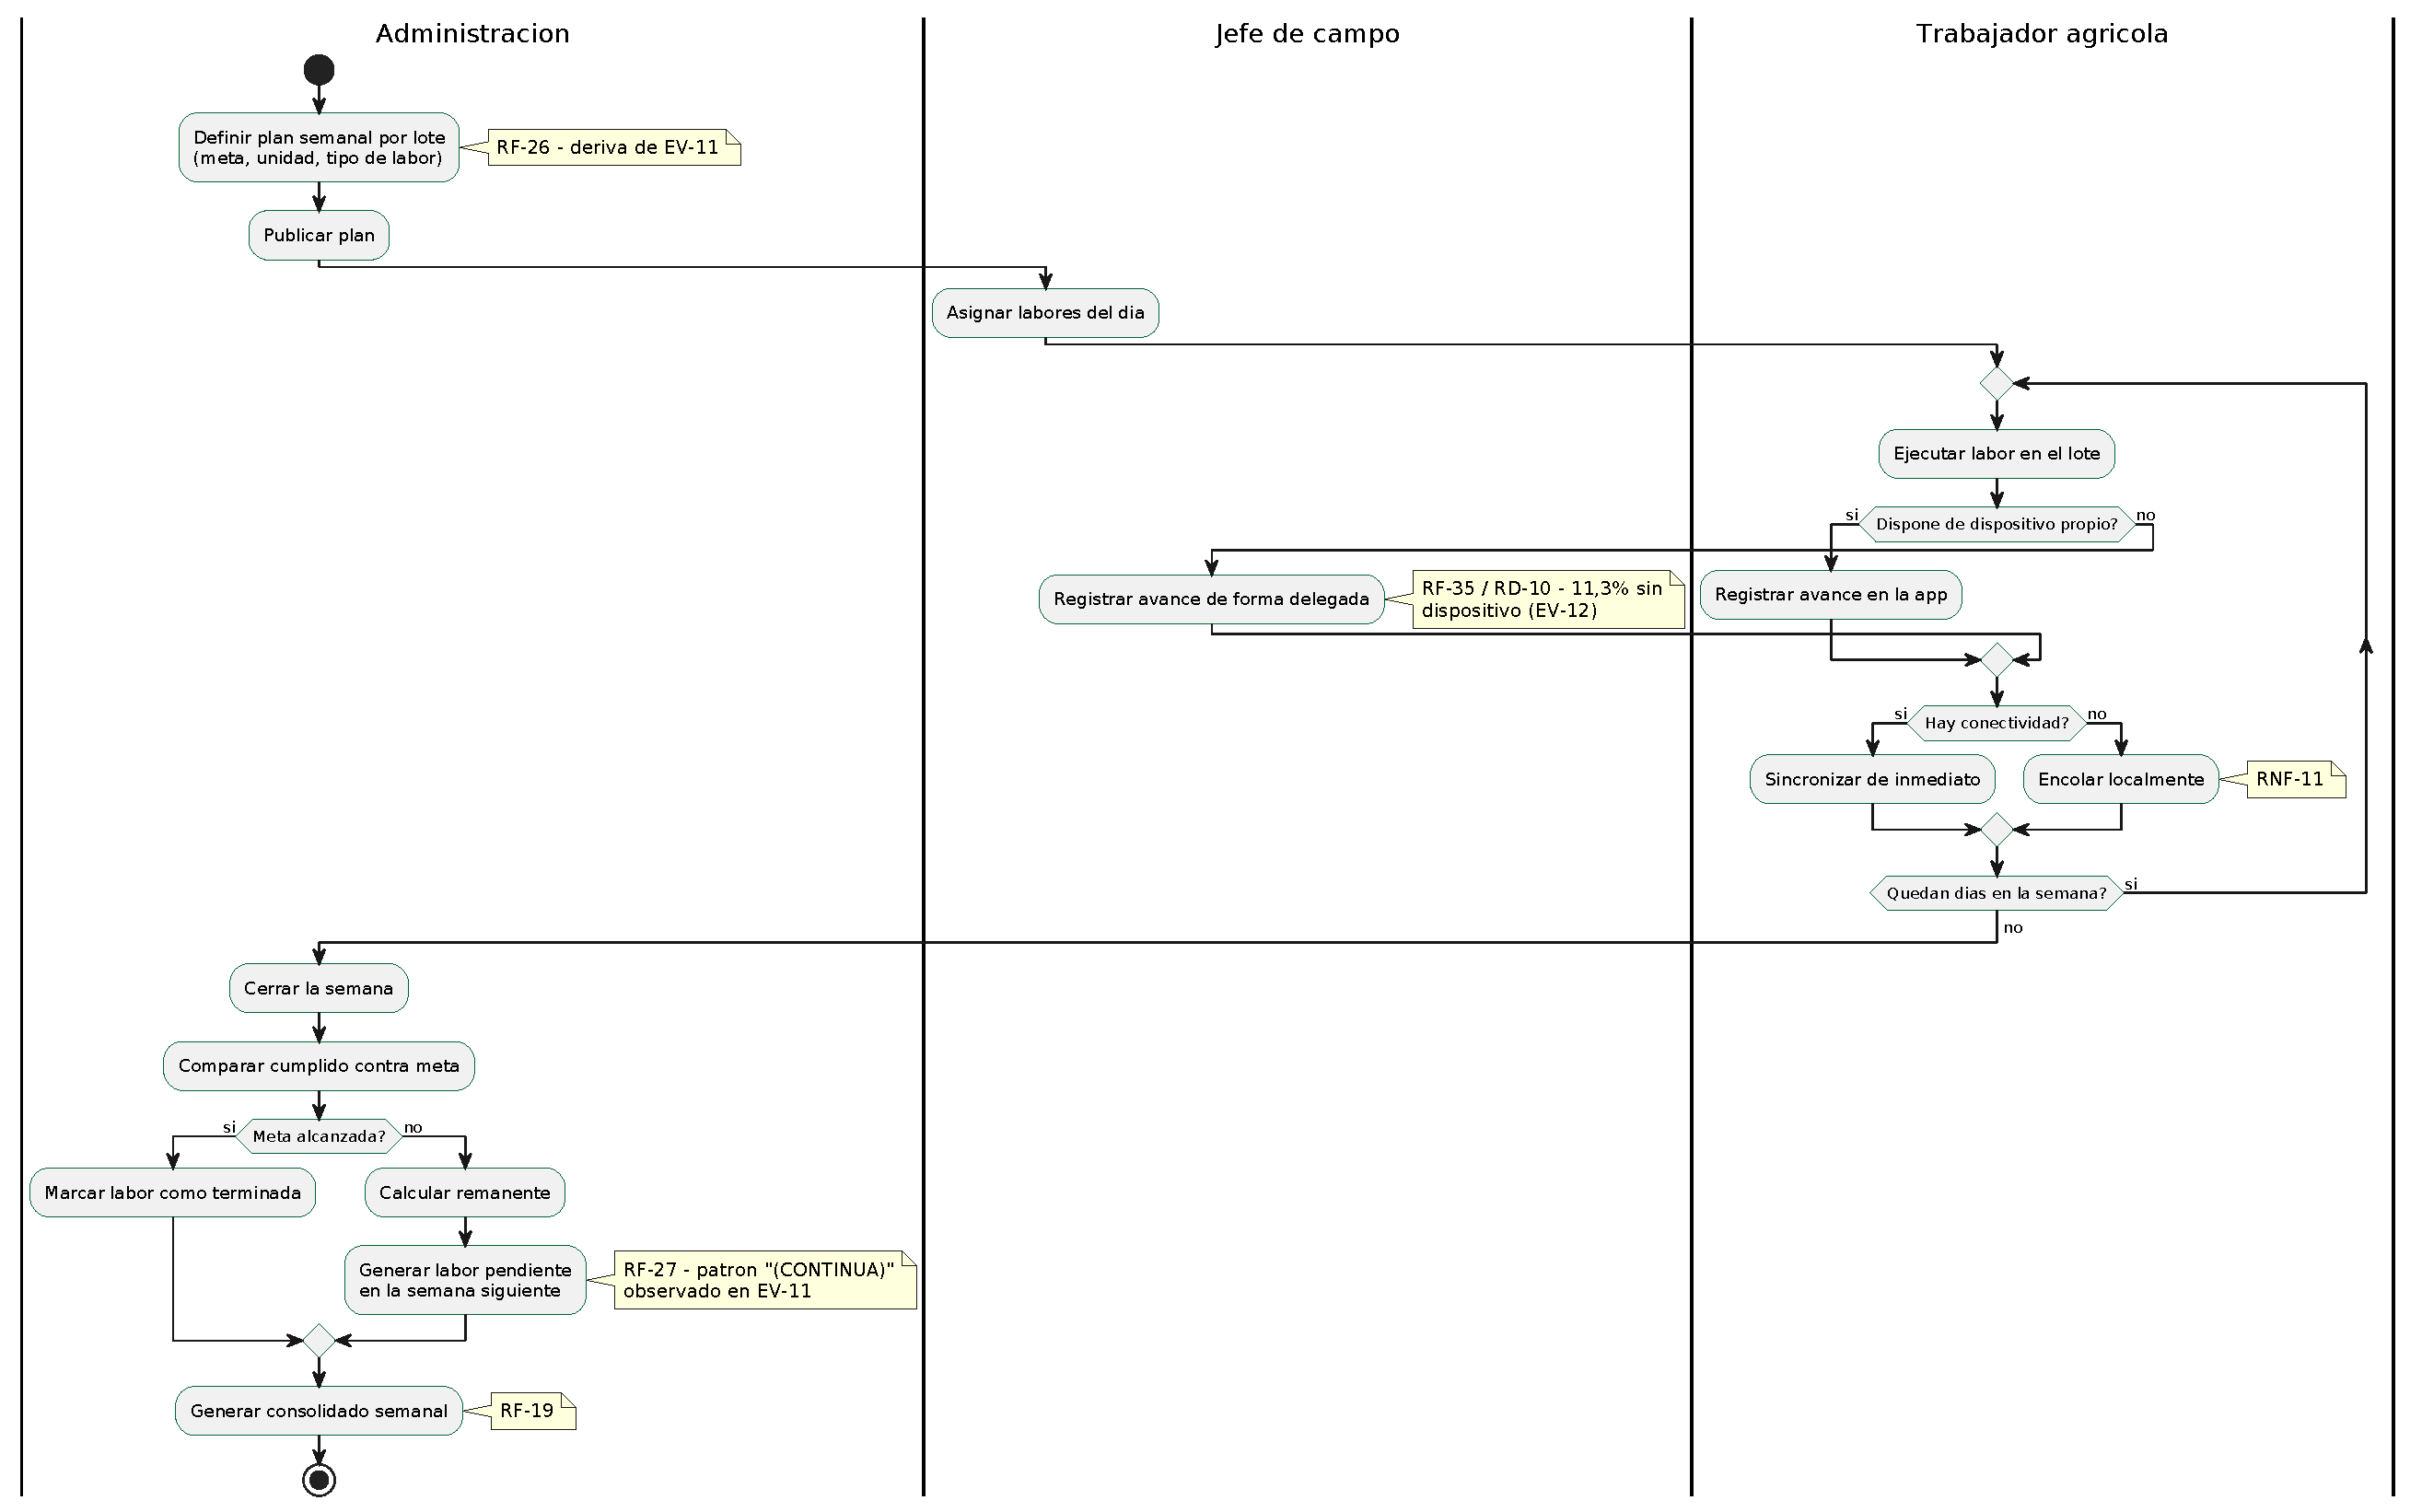
\includegraphics[width=1.0\textwidth]{img/actividad_ciclo_semanal}
\caption{Diagrama de actividad del ciclo semanal de planificación y ejecución de labores.}
\label{fig:actividad}
\end{figure}

% ---------------------------------------------------------------------
\subsection{Diagramas de estados}

Se modelan las dos entidades del dominio con ciclo de vida no trivial: el \textbf{racimo}, cuya
trayectoria determina el valor económico de la producción, y la \textbf{alerta}, cuyo ciclo refleja
la latencia real de verificación documentada en \id{EV-07}.

\begin{figure}[!htbp]
\centering
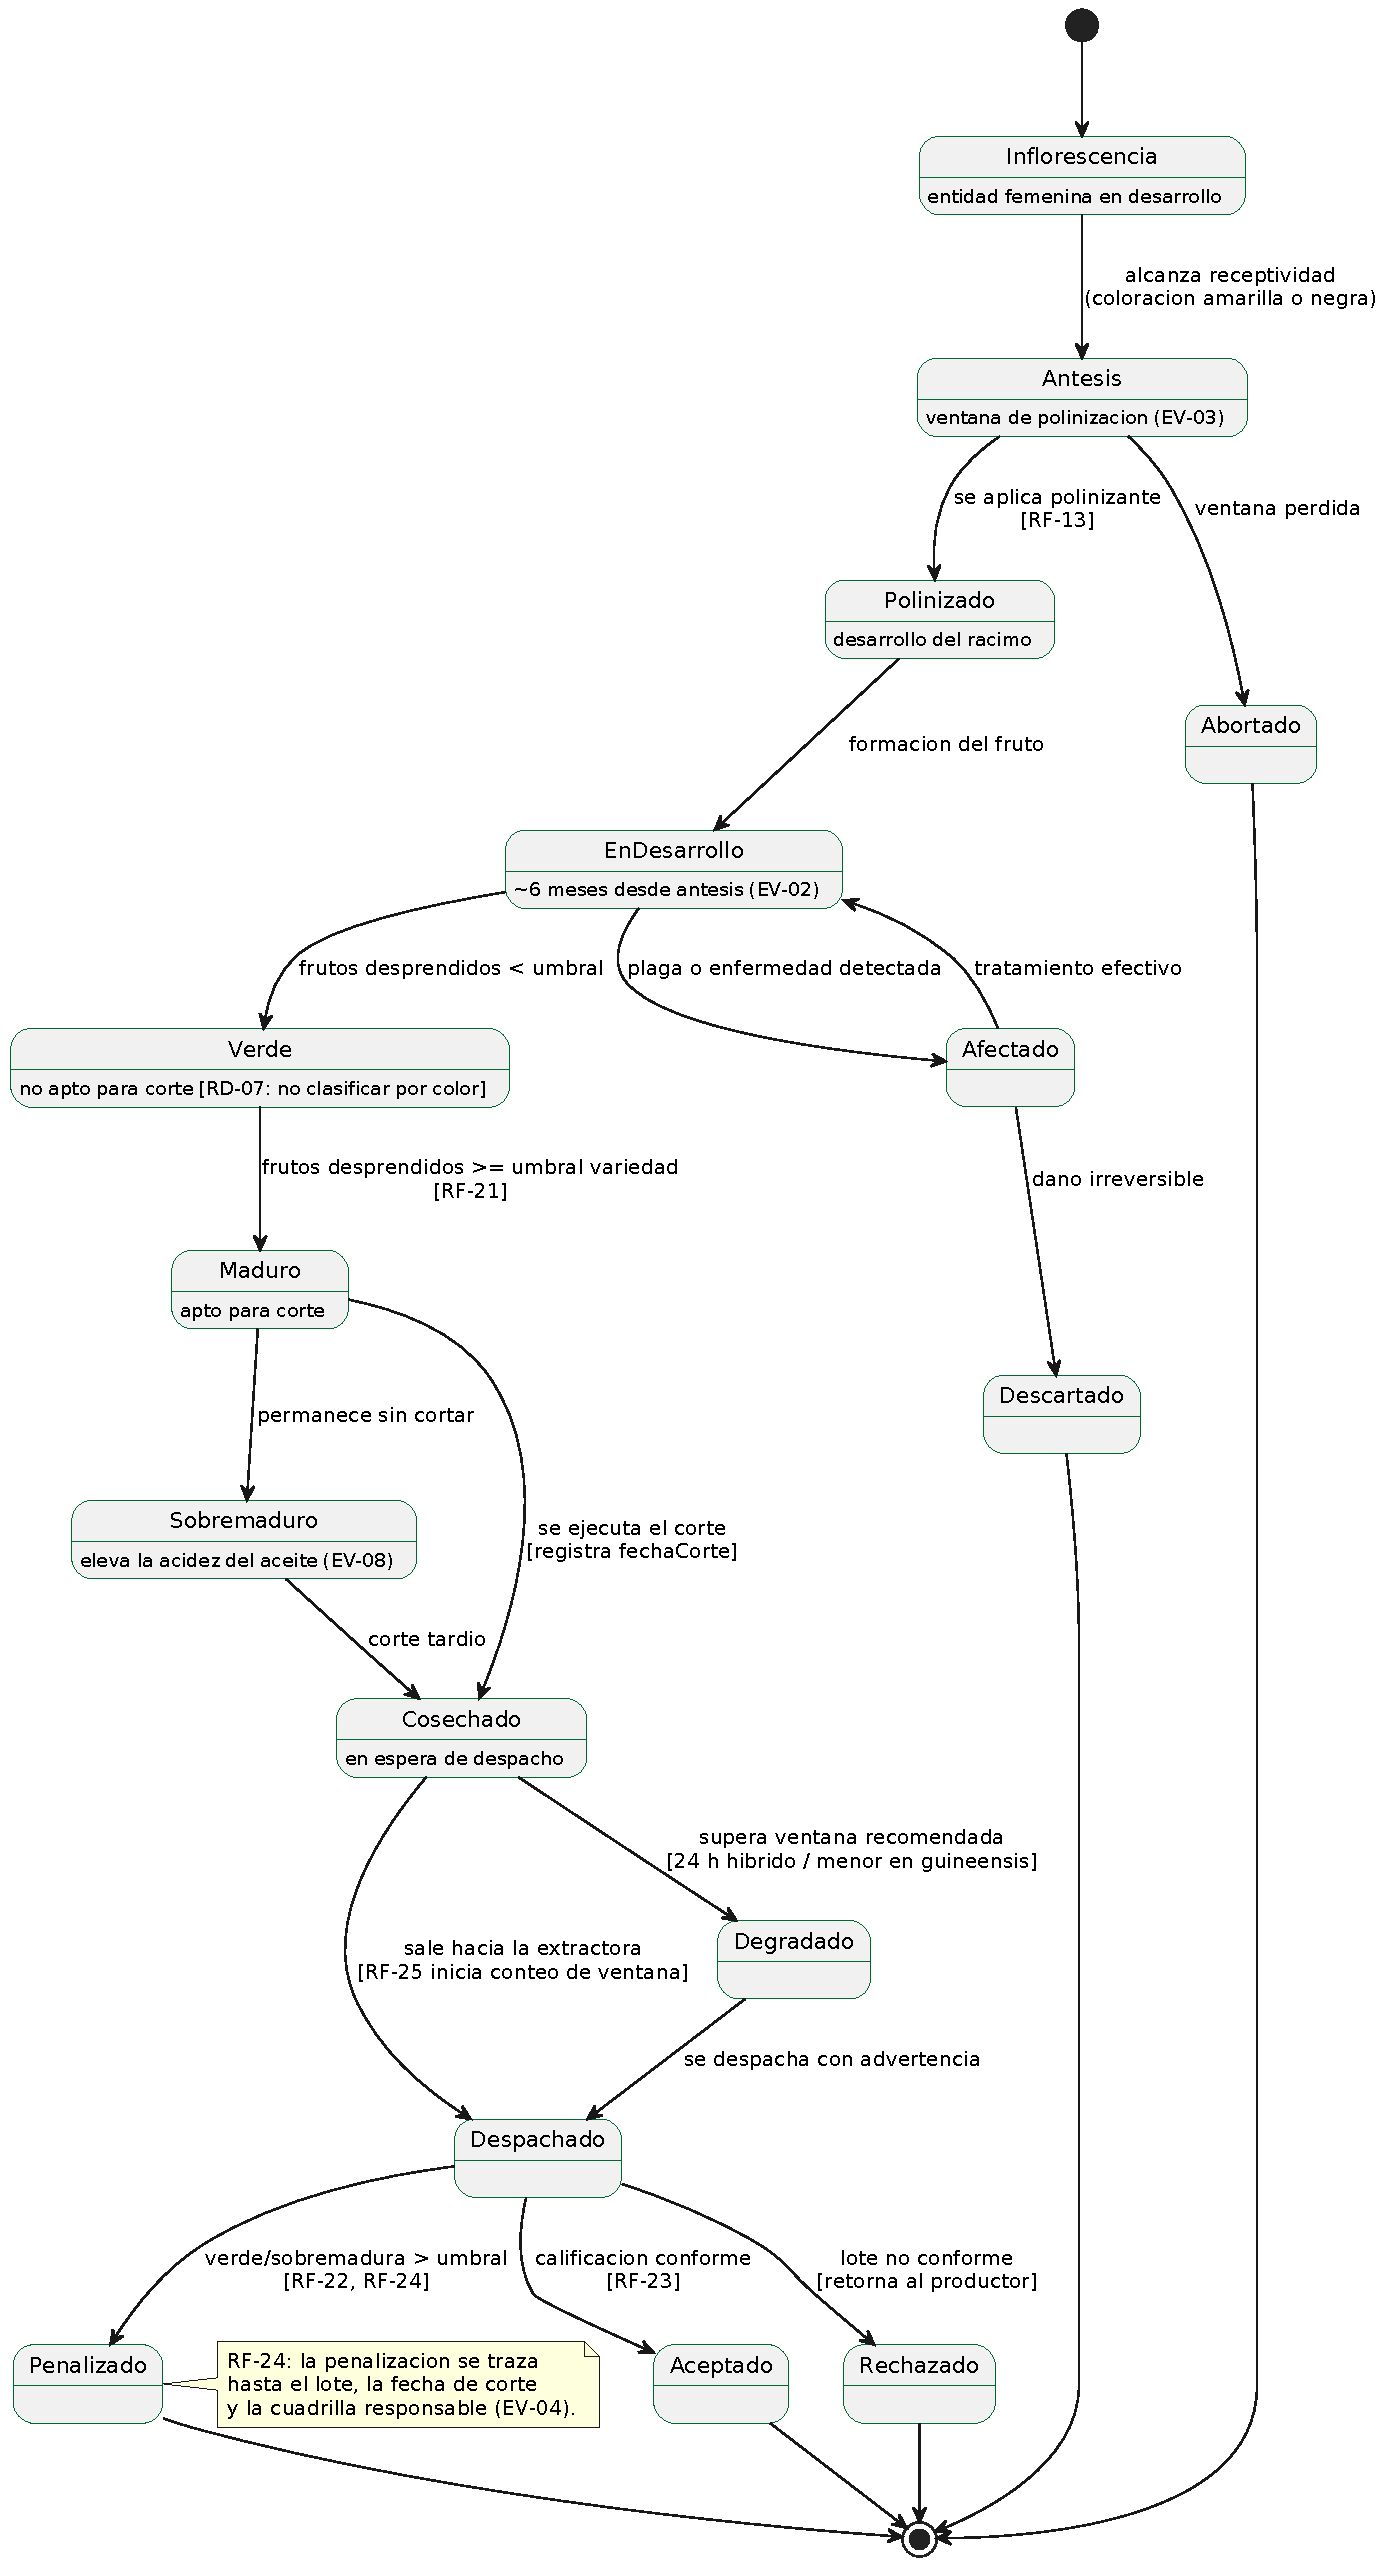
\includegraphics[width=0.67\textwidth]{img/estados_racimo}
\caption{Diagrama de estados del racimo, desde la inflorescencia hasta la calificación en la planta extractora.}
\label{fig:est_racimo}
\end{figure}

\begin{figure}[!htbp]
\centering
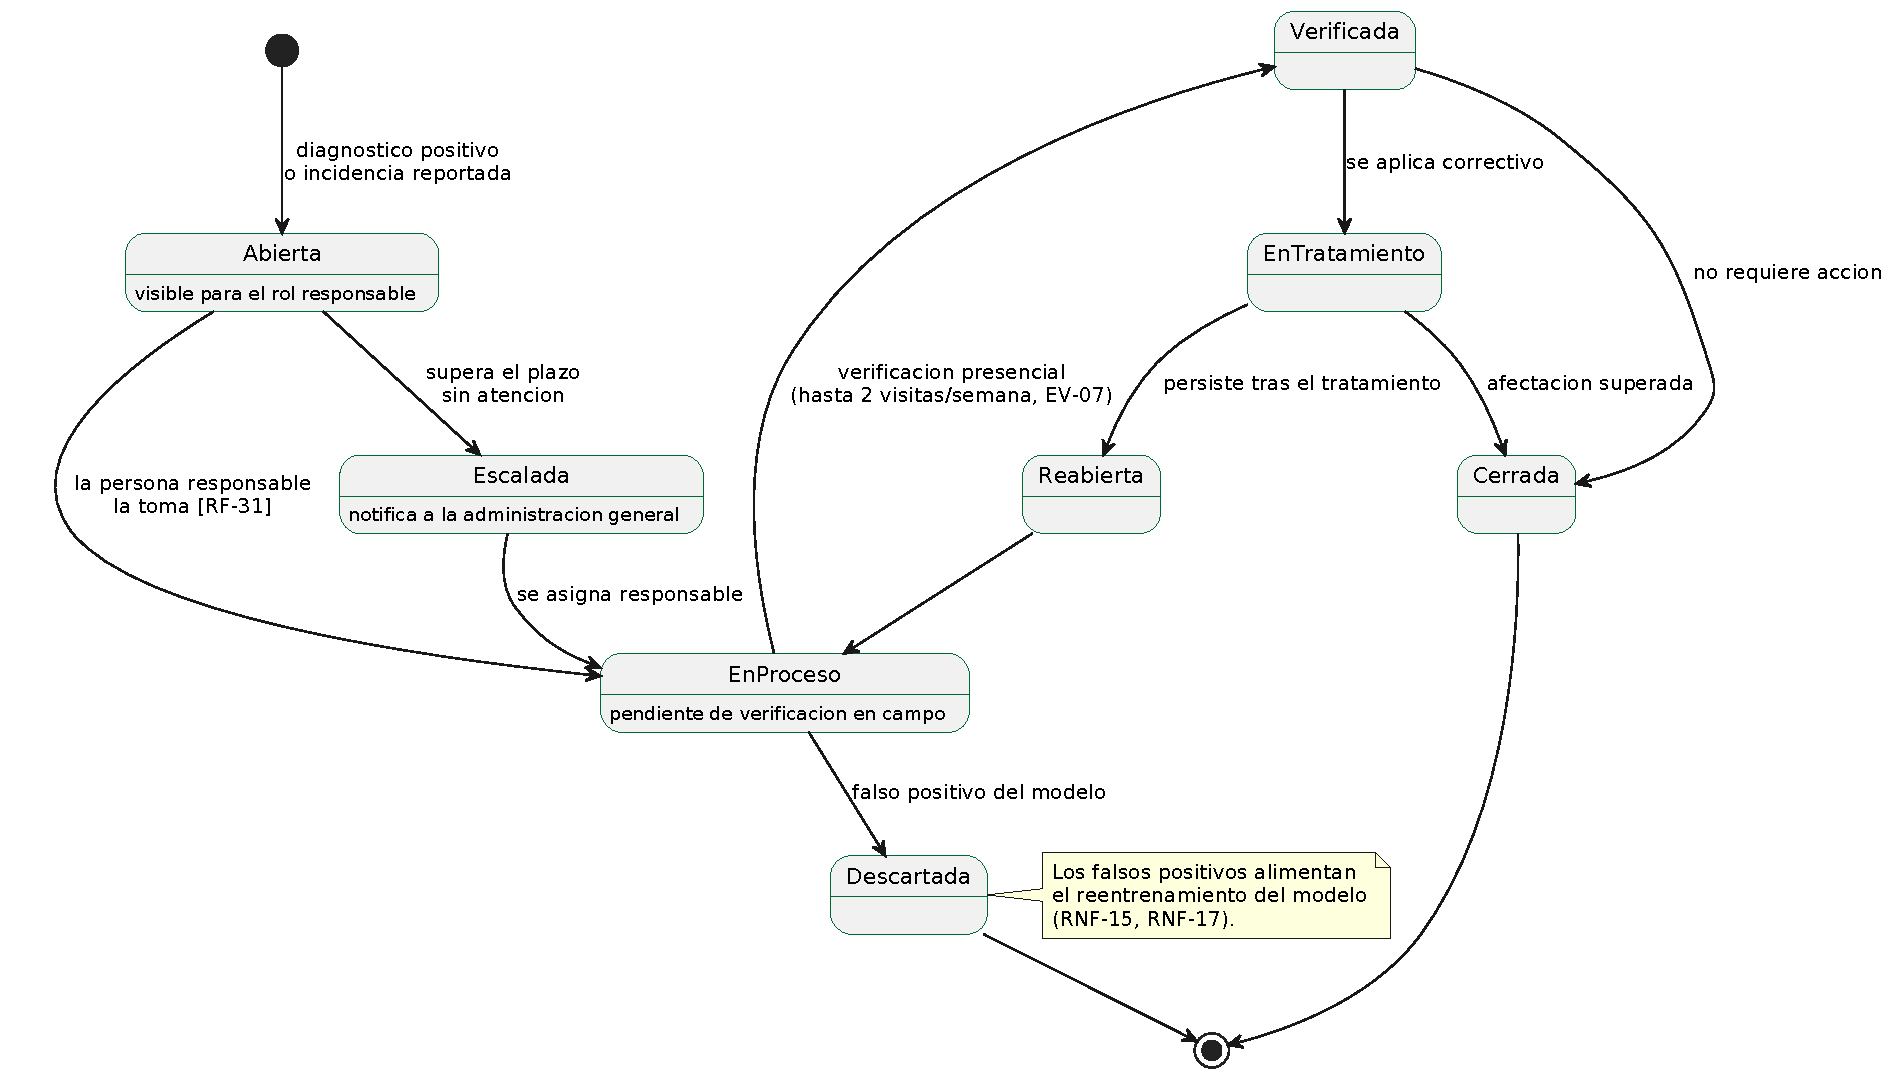
\includegraphics[width=1.0\textwidth]{img/estados_alerta}
\caption{Diagrama de estados de la alerta, con escalamiento por vencimiento de plazo y reapertura tras tratamiento inefectivo.}
\label{fig:est_alerta}
\end{figure}

\noindent
El estado \emph{Degradado} del racimo materializa el hallazgo de \id{EV-04} sobre la ventana entre
corte y entrega: el material híbrido tolera un intervalo mayor por su contenido de antioxidantes,
mientras que el \emph{guineensis} se deshidrata en dos o tres días. El estado \emph{Descartada} de
la alerta corresponde a los falsos positivos del modelo y alimenta el ciclo de reentrenamiento
previsto en \id{RNF-15} y \id{RNF-17}.

% ---------------------------------------------------------------------
\subsection{Diagrama de componentes}

\begin{figure}[!htbp]
\centering
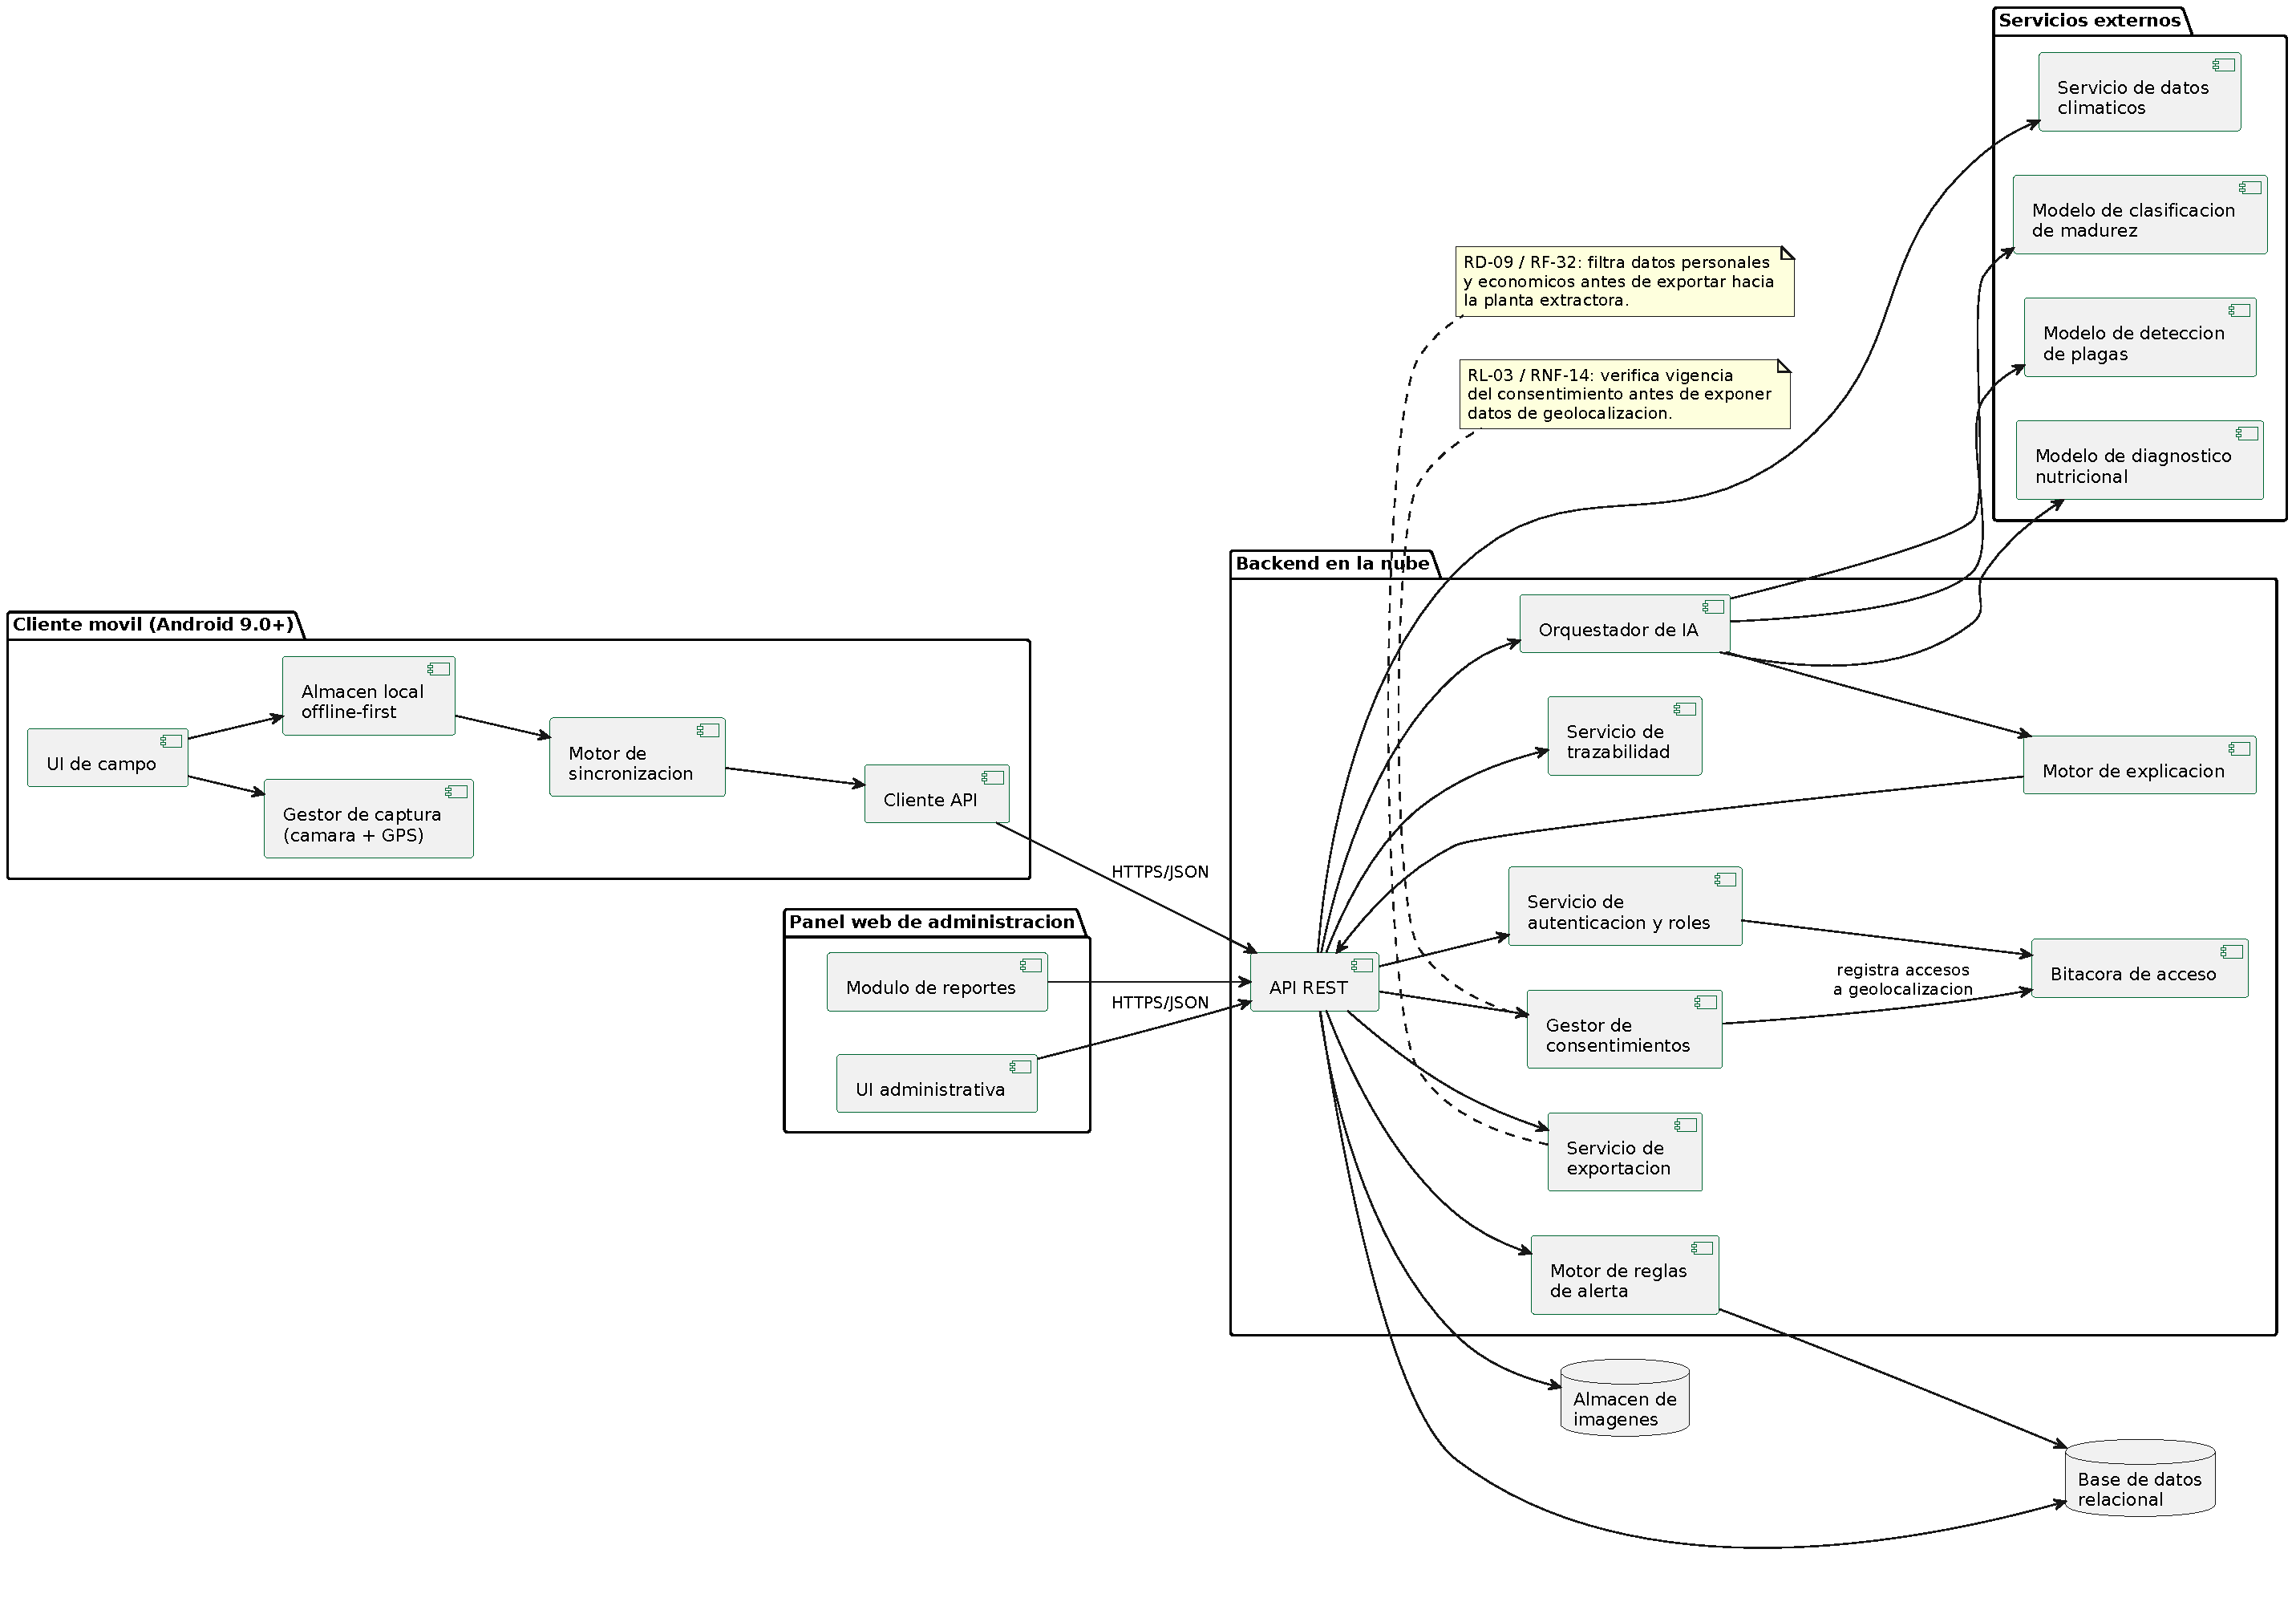
\includegraphics[width=1.0\textwidth]{img/componentes}
\caption{Diagrama de componentes del SIMPA.}
\label{fig:componentes}
\end{figure}

\noindent
Dos componentes merecen mención explícita por su origen normativo. El \emph{gestor de
consentimientos} verifica la vigencia antes de exponer cualquier dato de geolocalización y registra
todo acceso en la bitácora (\id{RL-03}, \id{RNF-14}). El \emph{servicio de exportación} filtra los
datos personales y económicos antes de generar el archivo destinado a la planta extractora
(\id{RD-09}, \id{RF-32}); su existencia como componente separado responde al criterio expreso de la
contraparte de que hay información que no puede compartirse (\id{EV-04}).

% ---------------------------------------------------------------------
\subsection{Diagrama de despliegue}

\begin{figure}[!htbp]
\centering
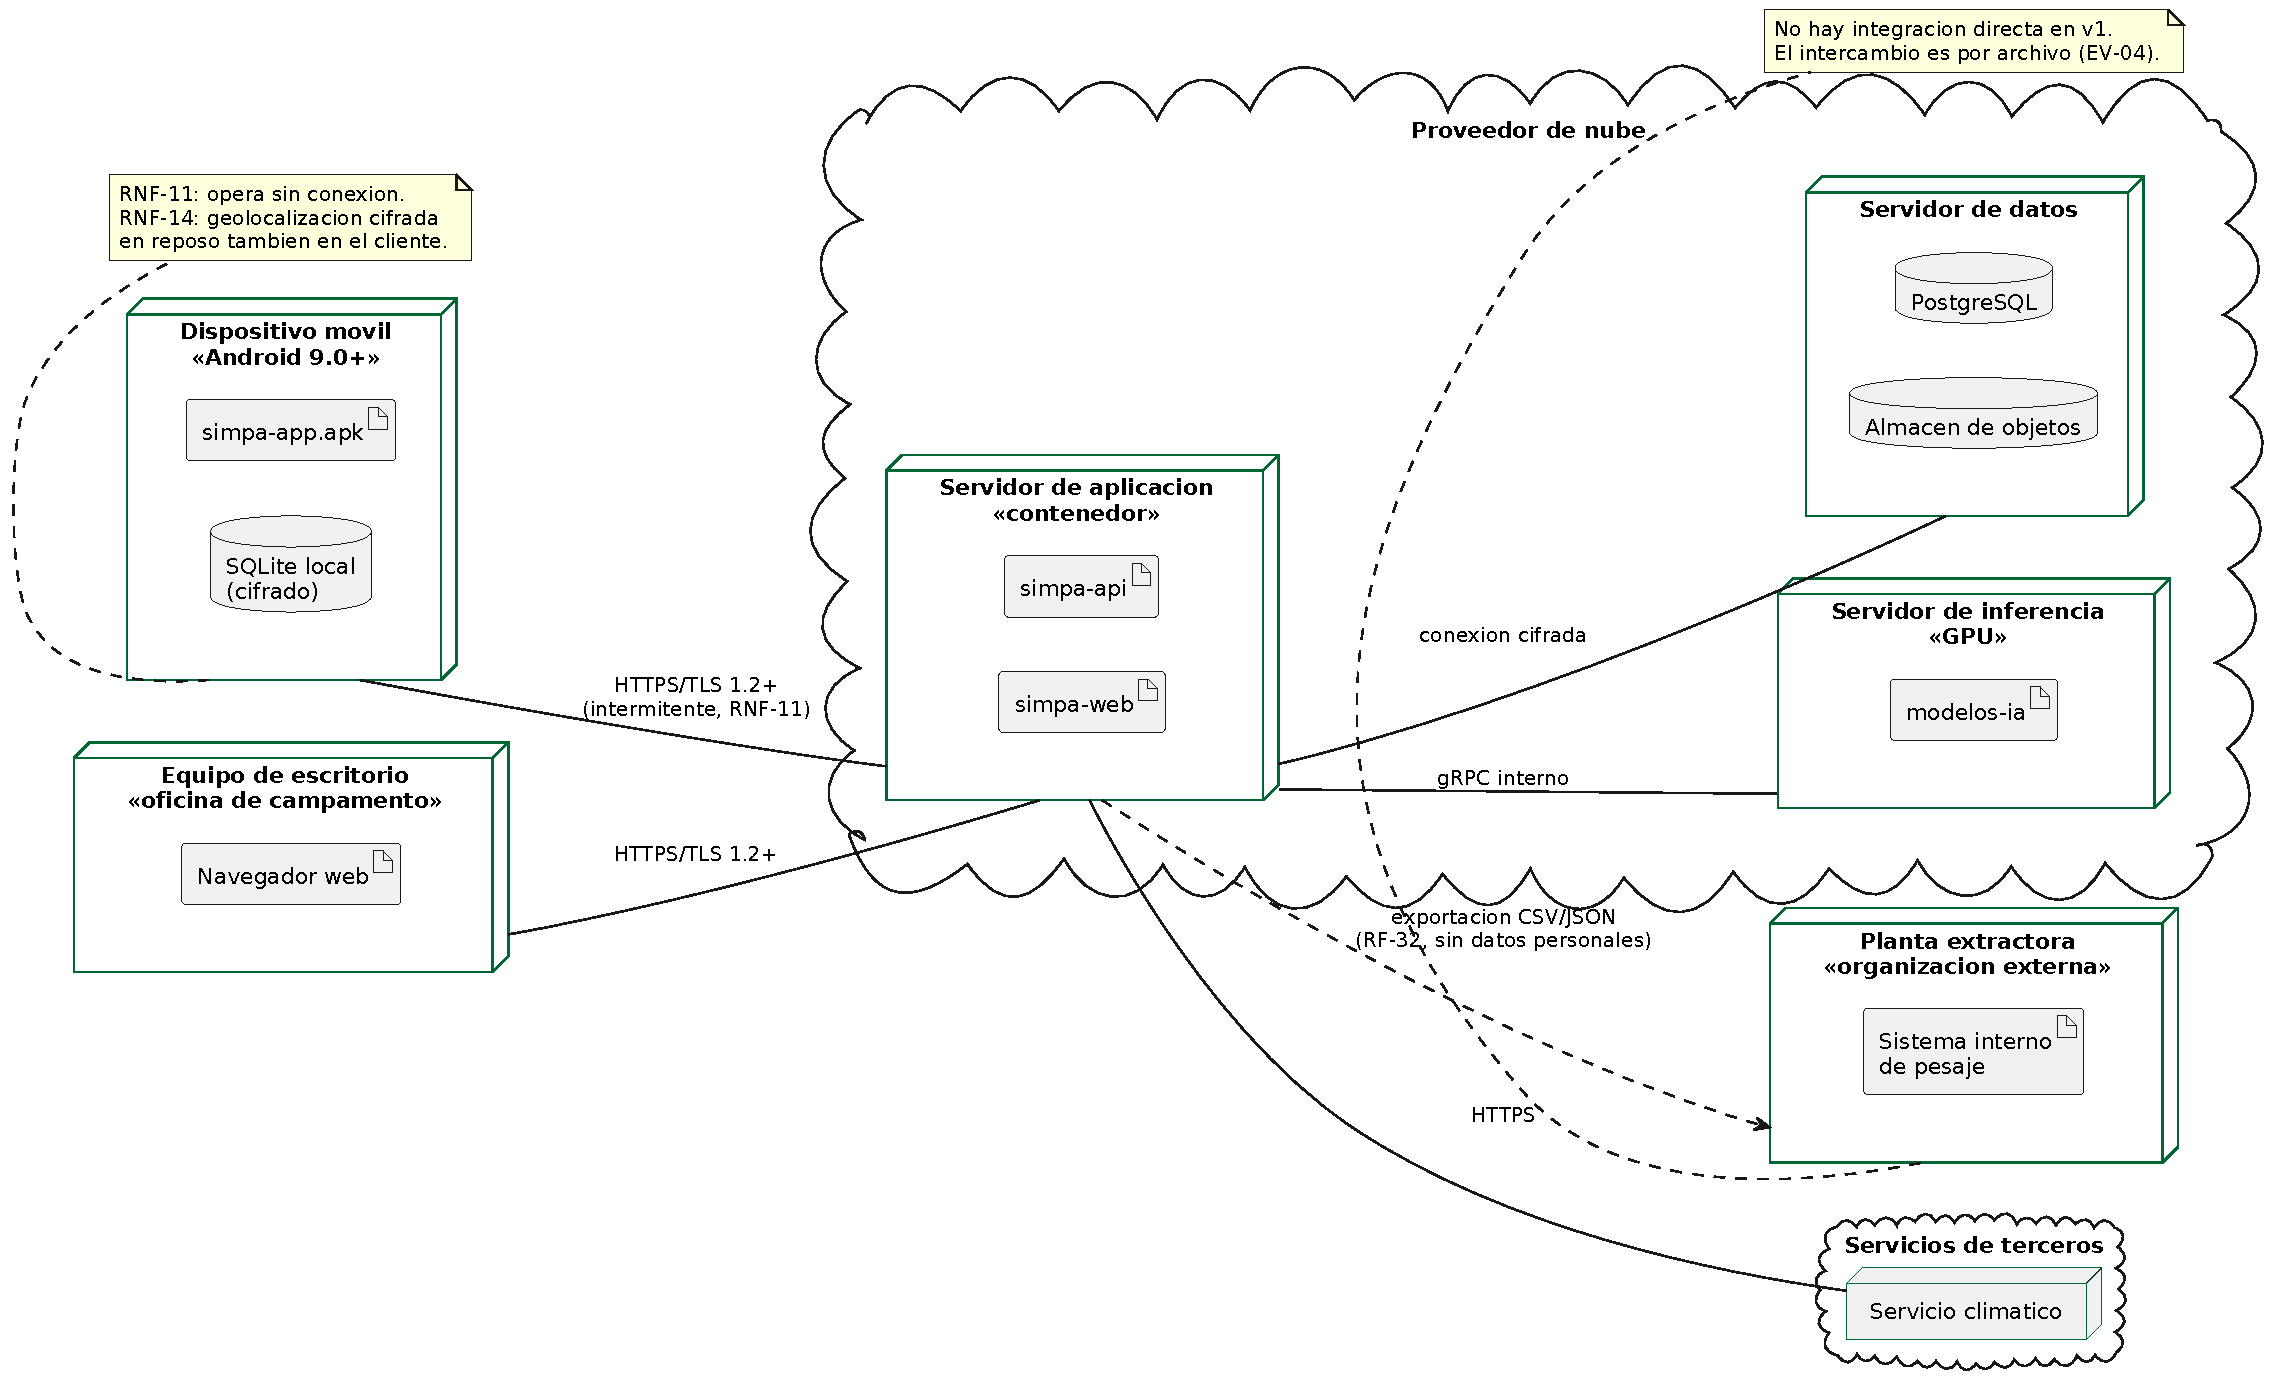
\includegraphics[width=1.0\textwidth]{img/despliegue}
\caption{Diagrama de despliegue del SIMPA.}
\label{fig:despliegue}
\end{figure}

\noindent
El enlace entre el dispositivo móvil y el servidor de aplicación se declara explícitamente como
\emph{intermitente}: el 74{,}2\% de las personas destinatarias no dispone de conectividad permanente
(\id{EV-12}). La planta extractora se representa como nodo externo sin integración directa; el
intercambio en la versión v1 se realiza por archivo, conforme a \id{RF-32}.

% ---------------------------------------------------------------------
\subsection{Cobertura del modelado}

\begin{longtable}{|L{4.6cm}|C{2.2cm}|C{2.2cm}|L{5.0cm}|}
\hline
\rowcolor{grisclaro}\textbf{Artefacto} & \textbf{Exigido} & \textbf{Entregado} & \textbf{Observación} \\
\hline
\endhead
Diagrama de casos de uso general & 1 & 1 & 8 actores, 18 casos de uso \\ \hline
Casos de uso detallados & 10 & 10 & Todos los \emph{Must}; $\geq 2$ flujos alternativos y $\geq 1$ excepción cada uno \\ \hline
Diagrama de clases refinado & 1 & 1 & 25 clases con atributos y operaciones \\ \hline
Diagramas de secuencia & CU \emph{Must} & 3 & CU-01, CU-03, CU-06 \\ \hline
Diagramas de actividad & Flujos principales & 1 & Ciclo semanal completo \\ \hline
Diagramas de estados & Entidades no triviales & 2 & Racimo y Alerta \\ \hline
Diagrama de componentes & 1 & 1 & --- \\ \hline
Diagrama de despliegue & 1 & 1 & --- \\ \hline
\caption{Cobertura del modelado UML frente a lo exigido en la §3.4 de la guía}
\end{longtable}

%  Requiere las imagenes en img/ generadas desde 03_Modelado/Diagramas_UML/
% =====================================================================

\newpage
\section{Modelado del sistema con UML}

El modelado emplea UML 2.5. Conforme a la §3.4 de la guía de la Entrega 3, se presentan ocho
diagramas: casos de uso general, especificación textual de diez casos de uso, clases refinado con
atributos y operaciones, tres diagramas de secuencia para los casos de uso \emph{Must}, actividad,
estados, componentes y despliegue. Todos se elaboraron en PlantUML y se entregan por triplicado
(fuente \id{.puml}, PNG a 300 dpi y SVG) en \id{03\_Modelado/Diagramas\_UML/}.

% ---------------------------------------------------------------------
\subsection{Diagrama general de casos de uso}

El diagrama presenta ocho actores y dieciocho casos de uso. Los actores primarios corresponden a los
seis perfiles de usuario de la §2.3; los actores secundarios son el servicio de análisis de IA y el
receptor GPS del dispositivo.

\begin{figure}[!htbp]
\centering
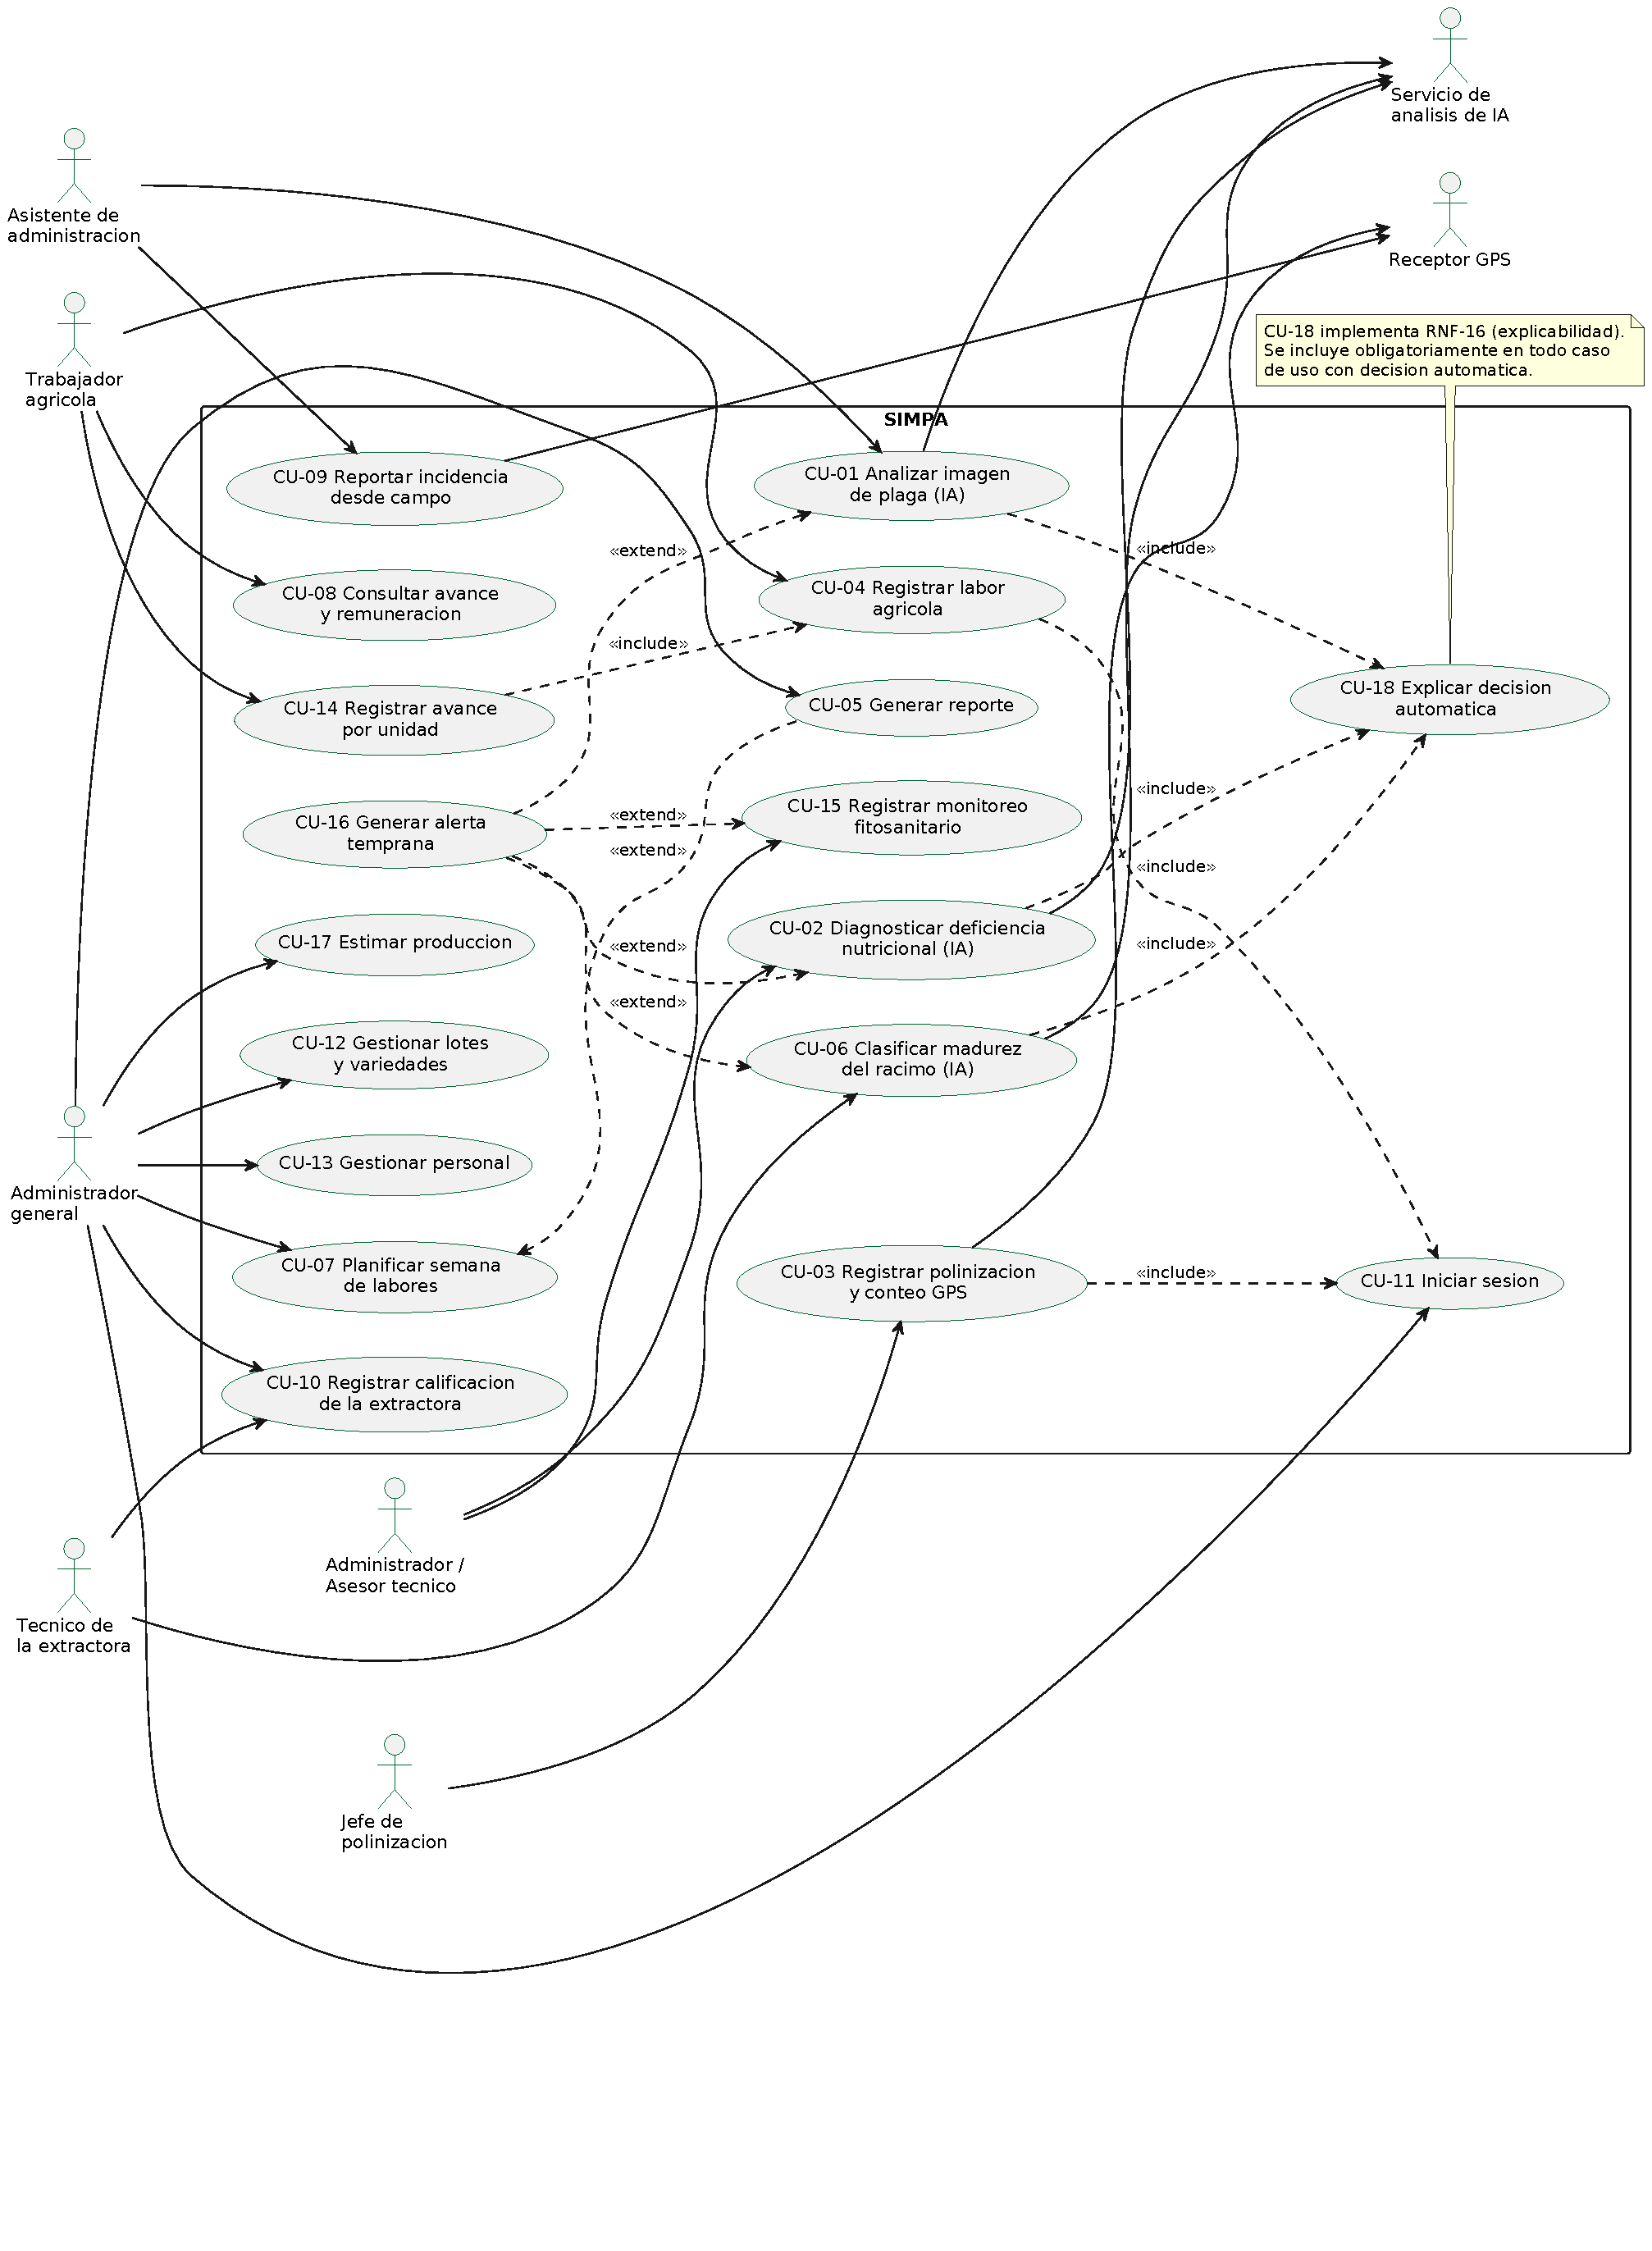
\includegraphics[width=0.91\textwidth]{img/casos_uso_general}
\caption{Diagrama general de casos de uso del SIMPA, con los ocho actores y el límite del sistema.}
\label{fig:cu_general}
\end{figure}

\noindent\textbf{Relaciones de inclusión y extensión.} \id{CU-14} incluye a \id{CU-04}, dado que el
registro de avance presupone una labor registrada. \id{CU-04} y \id{CU-03} incluyen a \id{CU-11},
por requerir sesión autenticada. Los tres casos de uso con decisión automática ---\id{CU-01},
\id{CU-02} y \id{CU-06}--- incluyen obligatoriamente a \id{CU-18}, que materializa el requisito de
explicabilidad \id{RNF-16}: no existe decisión automática sin explicación asociada. \id{CU-16}
extiende a los casos de diagnóstico y de monitoreo, puesto que la alerta se genera únicamente si el
resultado es positivo.

% ---------------------------------------------------------------------
\subsection{Especificación textual de los casos de uso}

Se especifican diez casos de uso, correspondientes a la totalidad de los requisitos funcionales de
prioridad \emph{Must}. Cada especificación incluye actores, precondiciones, postcondiciones, flujo
principal, al menos un flujo alternativo y al menos una excepción.

% --- CU-01
\begin{longtable}{|L{3.4cm}|L{12.0cm}|}
\hline
\rowcolor{grisclaro}\multicolumn{2}{|l|}{\textbf{CU-01 --- Analizar imagen para detectar plaga o enfermedad}}\\
\hline
\textbf{Requisitos} & \id{RF-07}, \id{RF-09}, \id{RF-12}, \id{RNF-16} \\ \hline
\textbf{Actores} & Primario: técnico fitosanitario / asistente de administración. Secundario: servicio de análisis de IA. \\ \hline
\textbf{Precondición} & Persona usuaria autenticada; lote seleccionado; cámara disponible. \\ \hline
\textbf{Postcondición} & El diagnóstico y su explicación quedan registrados y asociados al lote y a la fecha. \\ \hline
\textbf{Flujo principal} & 1. La persona usuaria selecciona el lote y la opción \emph{Analizar imagen}. \newline 2. Captura la fotografía de la palma o de la hoja. \newline 3. El sistema valida la calidad de la imagen. \newline 4. El sistema envía la imagen al servicio de IA con los parámetros de la variedad del lote. \newline 5. El servicio devuelve la clase de afectación, el nivel de confianza y el rasgo visual determinante. \newline 6. El sistema genera la explicación conforme a \id{RNF-16}. \newline 7. El sistema muestra el resultado, la explicación y la recomendación de control, y registra el diagnóstico. \\ \hline
\textbf{Flujo alternativo A} & \emph{Sin conectividad.} En el paso 4 el sistema almacena la imagen localmente y encola el análisis; al restablecerse la conexión lo ejecuta y notifica el resultado (\id{RNF-11}). \\ \hline
\textbf{Flujo alternativo B} & \emph{Confianza insuficiente.} Si el nivel de confianza es inferior al umbral configurado, el sistema no emite clasificación: informa que el resultado no es concluyente y sugiere repetir la captura o consultar a la asesoría técnica. \\ \hline
\textbf{Excepción E1} & Imagen de calidad insuficiente: el sistema solicita repetir la captura indicando el defecto detectado. \\ \hline
\textbf{Excepción E2} & Servicio de IA no disponible: el análisis queda en estado pendiente y la persona usuaria es notificada. \\ \hline
\textbf{Extensión} & Si el resultado es positivo, se ejecuta \id{CU-16} (generar alerta temprana). \\ \hline
\caption{CU-01 --- Analizar imagen para detectar plaga o enfermedad}
\end{longtable}

% --- CU-02
\begin{longtable}{|L{3.4cm}|L{12.0cm}|}
\hline
\rowcolor{grisclaro}\multicolumn{2}{|l|}{\textbf{CU-02 --- Diagnosticar deficiencia nutricional por imagen}}\\
\hline
\textbf{Requisitos} & \id{RF-08}, \id{RF-11}, \id{RNF-16} \\ \hline
\textbf{Actores} & Primario: administrador / asesor técnico. Secundario: servicio de análisis de IA. \\ \hline
\textbf{Precondición} & Persona usuaria autenticada; lote seleccionado con variedad asignada. \\ \hline
\textbf{Postcondición} & El diagnóstico nutricional y su recomendación quedan registrados en el historial del lote. \\ \hline
\textbf{Flujo principal} & 1. La persona usuaria selecciona \emph{Diagnóstico nutricional} y el lote. \newline 2. Captura la fotografía de la hoja. \newline 3. El sistema valida la imagen y la envía al servicio de IA. \newline 4. El servicio estima el elemento deficiente. \newline 5. El sistema genera una explicación de tipo causal, indicando qué signo foliar sustenta la estimación. \newline 6. El sistema muestra la deficiencia, la recomendación de fertilización y la explicación, y registra el diagnóstico. \\ \hline
\textbf{Flujo alternativo A} & La persona usuaria adjunta una imagen existente de la galería en lugar de capturarla. \\ \hline
\textbf{Flujo alternativo B} & \emph{Contraste con análisis de laboratorio.} Si el lote tiene un análisis de suelo o foliar registrado (\id{RF-11}), el sistema contrasta la estimación con los valores medidos y señala la discrepancia si la hubiere. \\ \hline
\textbf{Excepción E1} & Imagen no válida: el sistema solicita repetir la captura. \\ \hline
\textbf{Excepción E2} & Lote sin variedad asignada: el sistema advierte que la estimación puede no ser aplicable y solicita completar el dato. \\ \hline
\textbf{Extensión} & Si la deficiencia estimada es severa, se ejecuta \id{CU-16}. \\ \hline
\caption{CU-02 --- Diagnosticar deficiencia nutricional por imagen}
\end{longtable}

% --- CU-03
\begin{longtable}{|L{3.4cm}|L{12.0cm}|}
\hline
\rowcolor{grisclaro}\multicolumn{2}{|l|}{\textbf{CU-03 --- Registrar polinización y conteo georreferenciado}}\\
\hline
\textbf{Requisitos} & \id{RF-13}, \id{RF-14}, \id{RNF-05}, \id{RNF-12}, \id{RL-03} \\ \hline
\textbf{Actores} & Primario: polinizador. Secundario: receptor GPS. \\ \hline
\textbf{Precondición} & Lote en etapa de polinización; sesión iniciada; consentimiento de geolocalización vigente. \\ \hline
\textbf{Postcondición} & La polinización y el conteo diario quedan registrados por persona, lote y fecha, sin ingreso manual planta por planta. \\ \hline
\textbf{Flujo principal} & 1. El polinizador inicia la jornada en el lote. \newline 2. El sistema verifica la vigencia del consentimiento de geolocalización. \newline 3. El sistema activa el rastreo con período de muestreo de 30 s. \newline 4. Durante la jornada, el sistema almacena las marcaciones georreferenciadas. \newline 5. El polinizador registra el estado de la antesis y la verificación visual. \newline 6. Al cierre, el sistema calcula el número de flores polinizadas a partir de las marcaciones. \newline 7. El sistema almacena el registro y muestra el total a la persona trabajadora. \\ \hline
\textbf{Flujo alternativo A} & \emph{Consentimiento revocado.} Si el consentimiento no está vigente, el sistema no activa el rastreo y habilita el registro manual del número de flores, sin penalización para la persona trabajadora (\id{RL-03}). \\ \hline
\textbf{Flujo alternativo B} & \emph{Sin conectividad.} Las marcaciones se almacenan localmente y se sincronizan al reconectar (\id{RNF-11}). \\ \hline
\textbf{Excepción E1} & Precisión GPS superior a 10 m: el sistema conserva el dato marcándolo como de precisión degradada y advierte a la persona usuaria, sin descartar la jornada (\id{RNF-12}). \\ \hline
\textbf{Excepción E2} & Pérdida total de señal GPS durante la jornada: el sistema conserva el tramo registrado y solicita completar el conteo de forma manual para el tramo faltante. \\ \hline
\caption{CU-03 --- Registrar polinización y conteo georreferenciado}
\end{longtable}

% --- CU-04
\begin{longtable}{|L{3.4cm}|L{12.0cm}|}
\hline
\rowcolor{grisclaro}\multicolumn{2}{|l|}{\textbf{CU-04 --- Registrar labor agrícola}}\\
\hline
\textbf{Requisitos} & \id{RF-04}, \id{RF-28}, \id{RF-35} \\ \hline
\textbf{Actores} & Primario: trabajador agrícola. Alternativo: jefe de campo (registro delegado). \\ \hline
\textbf{Precondición} & Lote y persona trabajadora registrados; persona usuaria autenticada. \\ \hline
\textbf{Postcondición} & La labor y su avance quedan en el historial del lote y computan para el cumplimiento del plan semanal. \\ \hline
\textbf{Flujo principal} & 1. La persona usuaria selecciona el lote y el tipo de labor. \newline 2. Ingresa la cantidad ejecutada en la unidad correspondiente. \newline 3. El sistema valida que la unidad corresponda al tipo de labor. \newline 4. El sistema registra la labor asociada al lote, la fecha y la persona responsable. \newline 5. El sistema actualiza el avance acumulado del período y el cumplimiento de la meta semanal. \\ \hline
\textbf{Flujo alternativo A} & \emph{Registro delegado.} Si la persona trabajadora no dispone de dispositivo propio, el jefe de campo registra el avance en su nombre; el sistema conserva en bitácora la identidad de quien efectuó el registro (\id{RF-35}, \id{RD-10}). \\ \hline
\textbf{Flujo alternativo B} & \emph{Sin conectividad.} La labor se almacena localmente y se sincroniza al reconectar. \\ \hline
\textbf{Excepción E1} & Datos incompletos: el sistema impide guardar y señala los campos faltantes. \\ \hline
\textbf{Excepción E2} & Unidad incompatible con el tipo de labor: el sistema rechaza el registro e indica la unidad esperada. \\ \hline
\caption{CU-04 --- Registrar labor agrícola}
\end{longtable}

% --- CU-05
\begin{longtable}{|L{3.4cm}|L{12.0cm}|}
\hline
\rowcolor{grisclaro}\multicolumn{2}{|l|}{\textbf{CU-05 --- Generar reporte}}\\
\hline
\textbf{Requisitos} & \id{RF-19}, \id{RF-26} \\ \hline
\textbf{Actores} & Primario: administrador general. \\ \hline
\textbf{Precondición} & Existen registros en el período seleccionado. \\ \hline
\textbf{Postcondición} & El reporte queda disponible para consulta o exportación. \\ \hline
\textbf{Flujo principal} & 1. La persona administradora selecciona el tipo de reporte y el período. \newline 2. El sistema consolida labores, avance, producción y alertas del período. \newline 3. El sistema genera y presenta el reporte. \newline 4. La persona administradora lo consulta o lo exporta a PDF o a hoja de cálculo. \\ \hline
\textbf{Flujo alternativo A} & Filtrado por lote, por equipo o por persona trabajadora. \\ \hline
\textbf{Flujo alternativo B} & \emph{Reporte de cumplimiento semanal.} El sistema contrasta el plan de la semana con lo ejecutado y destaca las metas no alcanzadas y su remanente. \\ \hline
\textbf{Excepción E1} & Sin registros en el período: el sistema informa la ausencia de datos y propone un período alternativo con información disponible. \\ \hline
\caption{CU-05 --- Generar reporte}
\end{longtable}

% --- CU-06
\begin{longtable}{|L{3.4cm}|L{12.0cm}|}
\hline
\rowcolor{grisclaro}\multicolumn{2}{|l|}{\textbf{CU-06 --- Clasificar la madurez del racimo}}\\
\hline
\textbf{Requisitos} & \id{RF-21}, \id{RF-22}, \id{RD-07}, \id{RD-08}, \id{RNF-01}, \id{RNF-16} \\ \hline
\textbf{Actores} & Primario: cosechador / técnico de la extractora. Secundario: servicio de análisis de IA. \\ \hline
\textbf{Precondición} & Lote con variedad asignada; persona usuaria autenticada. \\ \hline
\textbf{Postcondición} & La clasificación queda asociada al racimo, al lote y a la fecha, y actualiza el porcentaje estimado de fruta verde del lote. \\ \hline
\textbf{Flujo principal} & 1. La persona usuaria selecciona el lote y la opción \emph{Clasificar racimo}. \newline 2. El sistema recupera el umbral de desprendimiento de la variedad del lote. \newline 3. La persona usuaria captura la fotografía de la parte basal del racimo. \newline 4. El servicio de IA cuenta los frutos desprendidos, sin emplear el color como criterio (\id{RD-07}). \newline 5. El sistema compara el conteo con el umbral de la variedad y determina el estado. \newline 6. El sistema genera una explicación por contraste, indicando el conteo obtenido y el umbral aplicable. \newline 7. El sistema registra la clasificación y actualiza el porcentaje de fruta verde del lote. \\ \hline
\textbf{Flujo alternativo A} & \emph{Verificación previa al despacho.} La persona usuaria solicita el porcentaje estimado de fruta verde del lote; si alcanza o supera el umbral de penalización, el sistema emite alerta preventiva y desaconseja el despacho (\id{RF-22}). \\ \hline
\textbf{Flujo alternativo B} & \emph{Sobremadurez.} Si el conteo excede ampliamente el umbral, el sistema clasifica el racimo como sobremaduro y advierte sobre el incremento de acidez. \\ \hline
\textbf{Excepción E1} & Lote sin variedad asignada: el sistema no clasifica y solicita completar el dato, dado que el umbral depende de la variedad. \\ \hline
\textbf{Excepción E2} & Parte basal no visible en la imagen: el sistema solicita repetir la captura indicando el encuadre requerido. \\ \hline
\caption{CU-06 --- Clasificar la madurez del racimo}
\end{longtable}

% --- CU-07
\begin{longtable}{|L{3.4cm}|L{12.0cm}|}
\hline
\rowcolor{grisclaro}\multicolumn{2}{|l|}{\textbf{CU-07 --- Planificar la semana de labores}}\\
\hline
\textbf{Requisitos} & \id{RF-26}, \id{RF-27}, \id{RF-34}, \id{RF-37} a \id{RF-39} \\ \hline
\textbf{Actores} & Primario: administrador general. \\ \hline
\textbf{Precondición} & Lotes y tipos de labor registrados. \\ \hline
\textbf{Postcondición} & El plan de la semana queda publicado y disponible para el seguimiento diario. \\ \hline
\textbf{Flujo principal} & 1. La persona administradora crea el plan de la semana. \newline 2. Para cada lote, define las labores previstas con su meta y unidad. \newline 3. El sistema incorpora automáticamente los remanentes arrastrados de la semana anterior. \newline 4. La persona administradora registra los insumos requeridos. \newline 5. El sistema publica el plan y lo hace visible al jefe de campo. \\ \hline
\textbf{Flujo alternativo A} & \emph{Cierre de semana.} Al cierre, el sistema calcula el cumplimiento de cada meta; si es parcial, genera el remanente como labor pendiente de la semana siguiente, vinculada a la de origen (\id{RF-27}). \\ \hline
\textbf{Flujo alternativo B} & Ajuste del plan durante la semana en curso, conservando la versión previa en bitácora. \\ \hline
\textbf{Flujo alternativo C} & \emph{Liquidación y aprobación.} Al cierre, el sistema genera la liquidación que contrasta cantidad presupuestada, cantidad ejecutada, tarifa y valor por grupo de labor, totaliza el gasto presupuestado frente al real, e incorpora las labores no presupuestadas en su grupo diferenciado (\id{RF-37}, \id{RF-38}). La persona administradora aprueba la liquidación y el período queda cerrado (\id{RF-39}). \\ \hline
\textbf{Excepción E1} & Meta expresada en unidad incompatible con el tipo de labor: el sistema rechaza la meta e indica la unidad esperada. \\ \hline
\textbf{Excepción E2} & Existe un plan publicado para la misma semana: el sistema advierte y solicita confirmación antes de sustituirlo. \\ \hline
\caption{CU-07 --- Planificar la semana de labores}
\end{longtable}

% --- CU-08
\begin{longtable}{|L{3.4cm}|L{12.0cm}|}
\hline
\rowcolor{grisclaro}\multicolumn{2}{|l|}{\textbf{CU-08 --- Consultar avance acumulado y remuneración estimada}}\\
\hline
\textbf{Requisitos} & \id{RF-29}, \id{RF-36}, \id{RL-04} \\ \hline
\textbf{Actores} & Primario: trabajador agrícola. \\ \hline
\textbf{Precondición} & Existen registros de avance de la persona trabajadora en el período. \\ \hline
\textbf{Postcondición} & Se presenta el consolidado del período, sin posibilidad de edición por parte de la persona trabajadora. \\ \hline
\textbf{Flujo principal} & 1. La persona trabajadora accede a \emph{Mi avance}. \newline 2. Selecciona el período (quincena en curso por defecto). \newline 3. El sistema agrega sus registros de avance por tipo de labor. \newline 4. El sistema obtiene del catálogo la tarifa vigente de cada tipo de labor a la fecha de cada registro y calcula la remuneración estimada correspondiente al trabajo por avance. \newline 5. El sistema presenta el desglose por labor y el total estimado. \\ \hline
\textbf{Flujo alternativo A} & \emph{Ejercicio del derecho de acceso.} La persona trabajadora solicita la exportación de sus datos personales; el sistema genera el archivo conforme al Art. 12 de la LOPDP (\id{RL-04}). \\ \hline
\textbf{Flujo alternativo B} & \emph{Discrepancia.} La persona trabajadora marca un registro como discrepante; el sistema notifica a la administración sin modificar el dato original, y la corrección se tramita mediante \id{RL-05}. \\ \hline
\textbf{Excepción E1} & Sin registros en el período: el sistema informa la ausencia de datos. \\ \hline
\textbf{Excepción E2} & La labor carece de tarifa vigente en el catálogo (\id{RF-36}) a la fecha del registro: el sistema muestra el avance en unidades, omite la estimación monetaria e indica que la tarifa no está vigente para esa fecha. \\ \hline
\caption{CU-08 --- Consultar avance acumulado y remuneración estimada}
\end{longtable}

% --- CU-09
\begin{longtable}{|L{3.4cm}|L{12.0cm}|}
\hline
\rowcolor{grisclaro}\multicolumn{2}{|l|}{\textbf{CU-09 --- Reportar incidencia desde el campo}}\\
\hline
\textbf{Requisitos} & \id{RF-30}, \id{RF-31}, \id{RF-12} \\ \hline
\textbf{Actores} & Primario: asistente de administración / trabajador agrícola. Secundario: receptor GPS. \\ \hline
\textbf{Precondición} & Persona usuaria autenticada; cámara y GPS disponibles. \\ \hline
\textbf{Postcondición} & La incidencia queda registrada con fotografía y coordenadas, e incorporada a la lista de pendientes de verificación. \\ \hline
\textbf{Flujo principal} & 1. La persona usuaria selecciona \emph{Reportar incidencia}. \newline 2. Captura la fotografía de la afectación. \newline 3. El sistema obtiene las coordenadas del punto. \newline 4. La persona usuaria selecciona el lote y describe la afectación. \newline 5. El sistema registra la incidencia georreferenciada. \newline 6. El sistema la incorpora a la lista de pendientes de la persona supervisora. \\ \hline
\textbf{Flujo alternativo A} & \emph{Análisis asistido.} La persona usuaria solicita el análisis de la fotografía; se ejecuta \id{CU-01} y el diagnóstico se asocia a la incidencia. \\ \hline
\textbf{Flujo alternativo B} & \emph{Verificación en visita.} La persona supervisora recorre su lista de pendientes, ubica la incidencia por sus coordenadas y la marca como verificada o descartada. \\ \hline
\textbf{Excepción E1} & GPS no disponible: el sistema registra la incidencia solicitando la selección manual del lote y la marca como de ubicación aproximada. \\ \hline
\textbf{Excepción E2} & Sin conectividad: la incidencia se encola y se sincroniza al reconectar, conservando el instante original de captura. \\ \hline
\caption{CU-09 --- Reportar incidencia desde el campo}
\end{longtable}

% --- CU-10
\begin{longtable}{|L{3.4cm}|L{12.0cm}|}
\hline
\rowcolor{grisclaro}\multicolumn{2}{|l|}{\textbf{CU-10 --- Registrar la calificación de la planta extractora}}\\
\hline
\textbf{Requisitos} & \id{RF-23}, \id{RF-24}, \id{RF-25}, \id{RF-33} \\ \hline
\textbf{Actores} & Primario: administrador general. \\ \hline
\textbf{Precondición} & Existe un despacho registrado con su fecha de corte. \\ \hline
\textbf{Postcondición} & La calificación queda asociada al lote de origen y disponible para el análisis de trazabilidad. \\ \hline
\textbf{Flujo principal} & 1. La persona administradora selecciona el despacho. \newline 2. Ingresa los datos del ticket de pesaje: peso bruto, tara y neto. \newline 3. Ingresa la calificación de calidad: tamaño del fruto, porcentaje de fruta verde, sobremadura, malformación y pedúnculo largo. \newline 4. El sistema calcula el intervalo entre el corte y la entrega. \newline 5. El sistema registra la calificación y la asocia al lote de origen. \\ \hline
\textbf{Flujo alternativo A} & \emph{Análisis de trazabilidad.} Ante una calificación desfavorable, la persona administradora consulta la cadena lote $\rightarrow$ fecha de corte $\rightarrow$ cuadrilla, y contrasta con las labores del período para distinguir si el origen está en la cosecha o en el manejo del cultivo (\id{RF-24}). \\ \hline
\textbf{Flujo alternativo B} & \emph{Ausencia de guía de remisión.} Si el despacho se registra sin número de guía, el sistema advierte antes del cierre (\id{RF-33}). \\ \hline
\textbf{Excepción E1} & El intervalo entre corte y entrega supera el valor recomendado para la variedad: el sistema registra la advertencia junto al despacho (\id{RF-25}). \\ \hline
\textbf{Excepción E2} & La suma de pesos es inconsistente (neto distinto de bruto menos tara): el sistema rechaza el registro e indica la inconsistencia. \\ \hline
\caption{CU-10 --- Registrar la calificación de la planta extractora}
\end{longtable}

% ---------------------------------------------------------------------
\subsection{Diagrama de clases refinado}

El modelo del dominio comprende veinticinco clases con atributos y operaciones. Incorpora tres
jerarquías de herencia (\id{Persona}--\id{Usuario} y la especialización de \id{Diagnostico} en sus
tres variantes), cuatro relaciones de composición y asociaciones con multiplicidad explícita. No
corresponde a un diseño de base de datos, sino al modelo conceptual del dominio del problema.

\begin{figure}[!htbp]
\centering
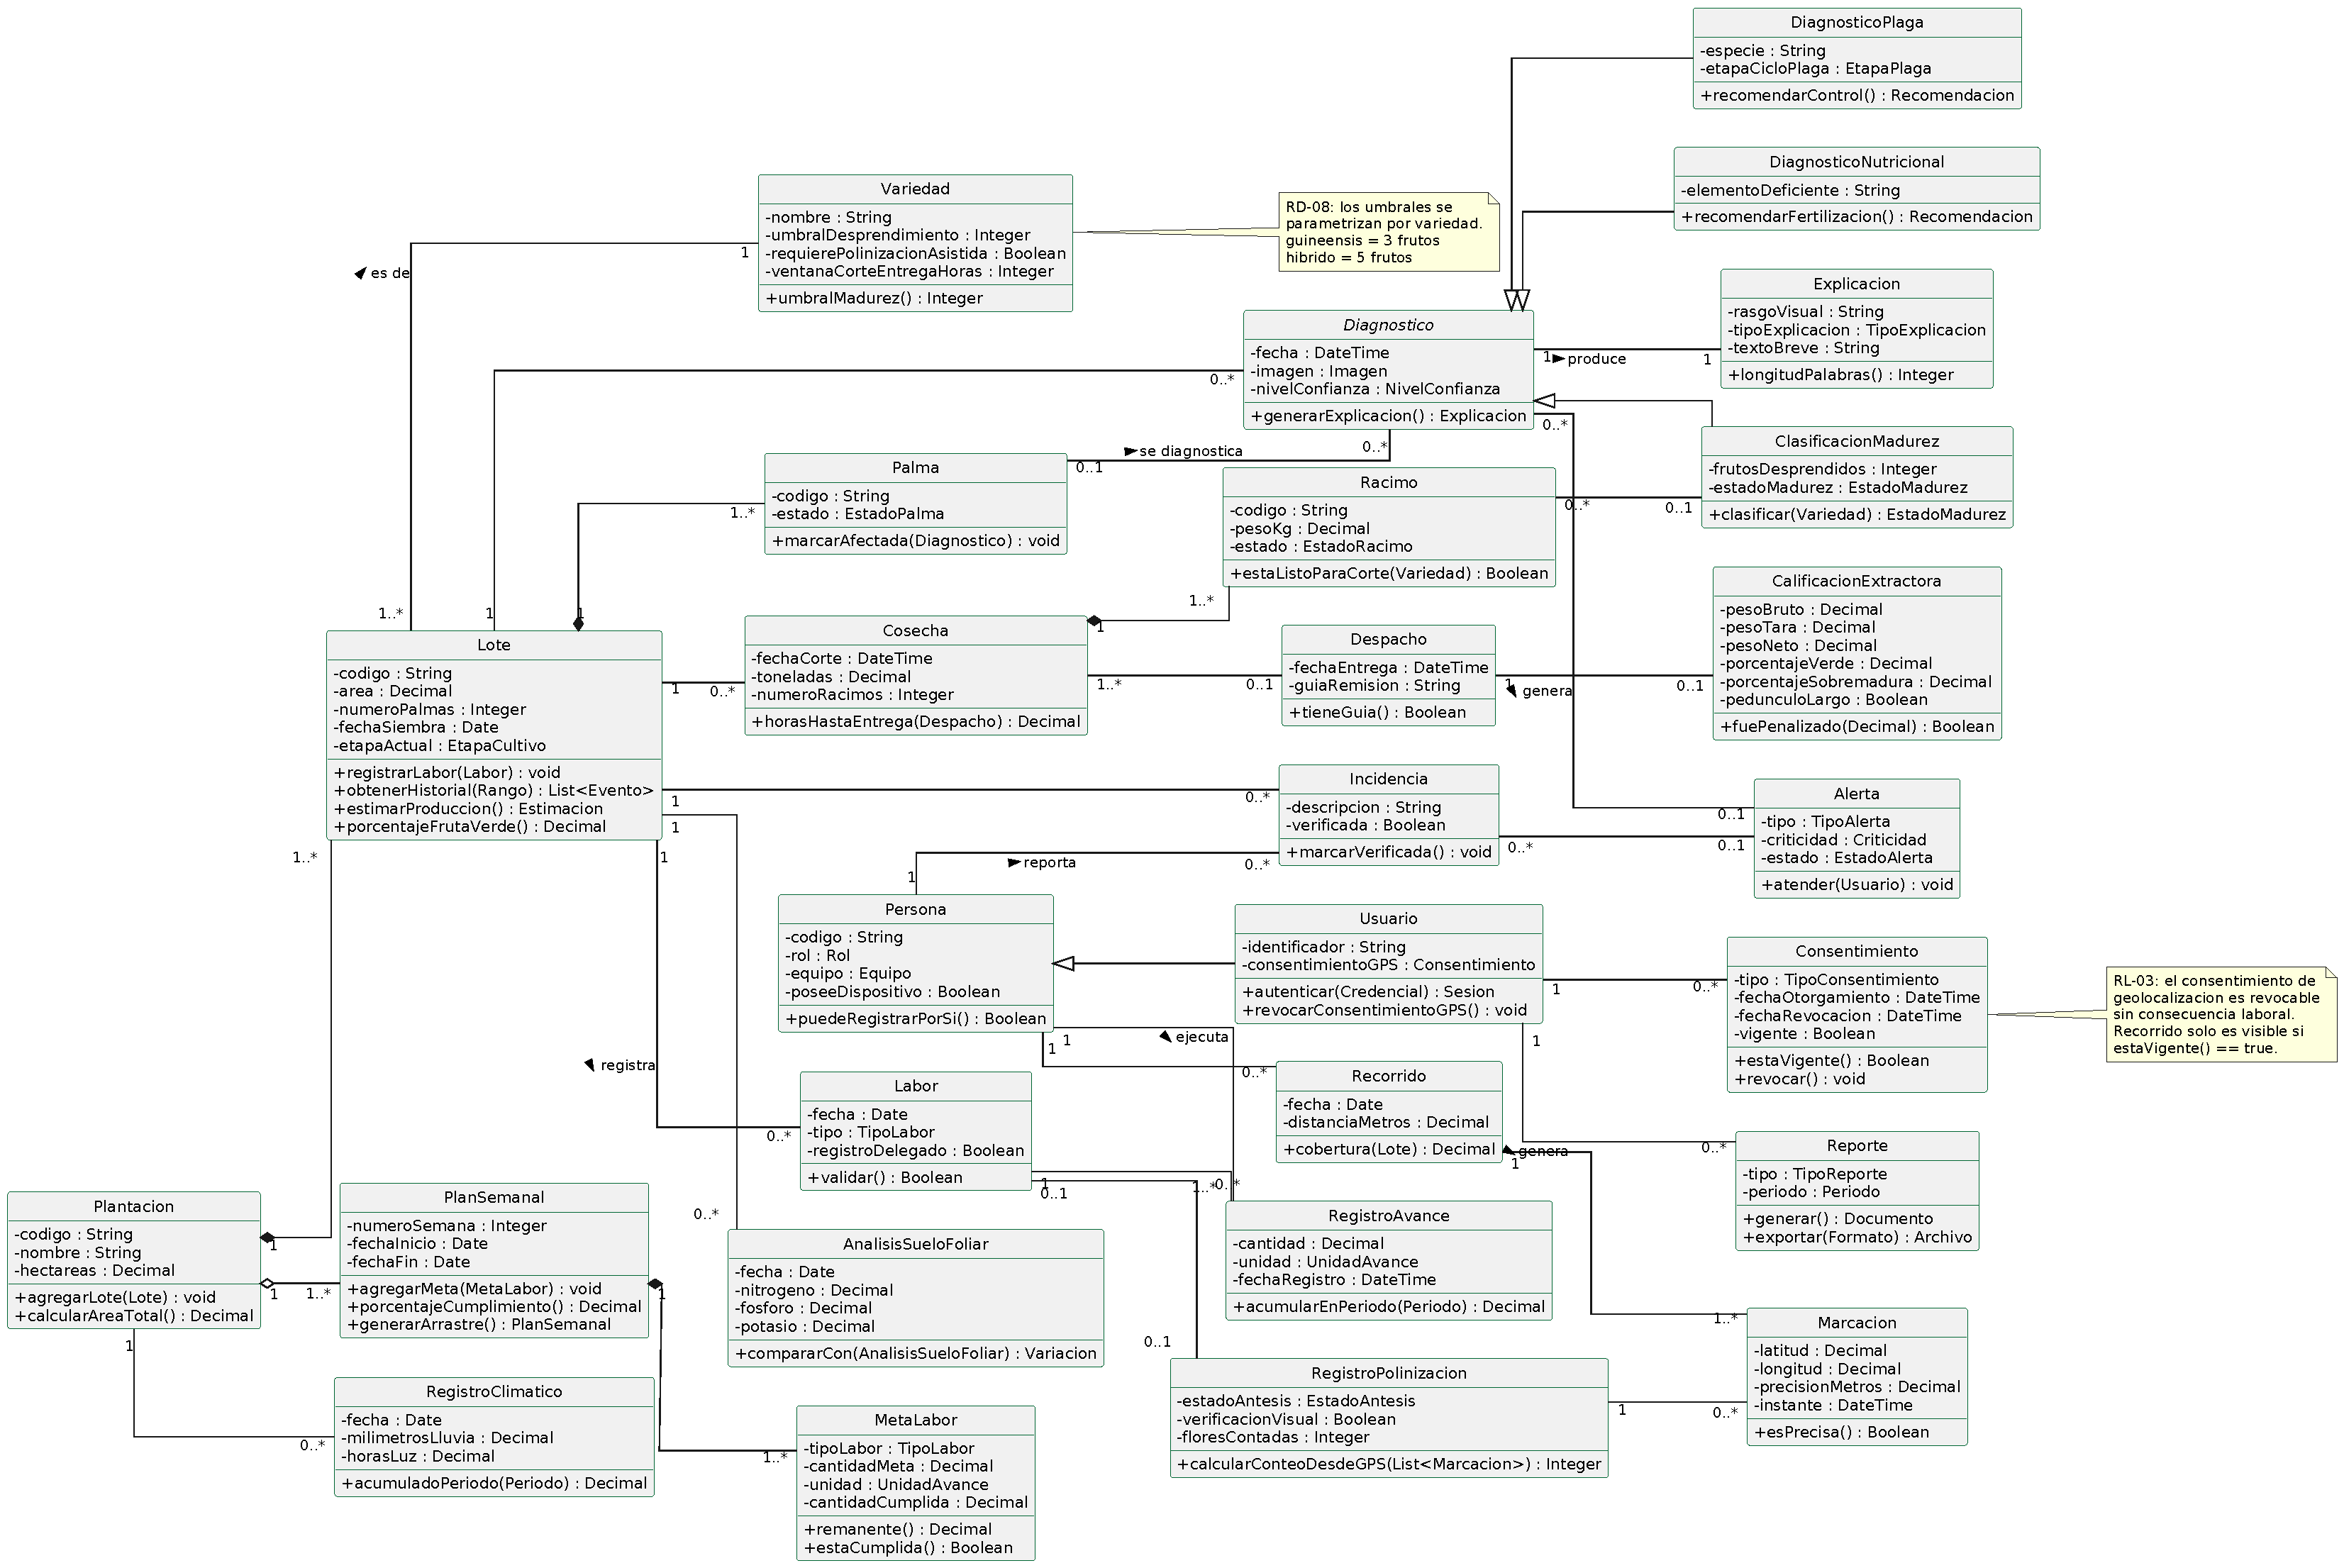
\includegraphics[width=1.0\textwidth]{img/clases_refinado}
\caption{Diagrama de clases refinado del SIMPA, con atributos y operaciones.}
\label{fig:clases}
\end{figure}

\noindent\textbf{Decisiones de modelado relevantes.} La clase \id{Consentimiento} se modela como
entidad de primer orden y no como atributo booleano de \id{Usuario}, porque el Art. 7 de la LOPDP
exige que el consentimiento sea específico por finalidad y revocable, lo que obliga a conservar su
historia. La clase \id{Variedad} concentra los umbrales de decisión ---desprendimiento, ventana
corte-entrega y necesidad de polinización asistida--- en lugar de fijarlos en la lógica de los
módulos de IA, conforme a \id{RD-08}. La clase \id{Explicacion} se asocia de forma obligatoria a
\id{Diagnostico} con multiplicidad 1:1, de modo que el modelo impide estructuralmente la existencia
de una decisión automática sin explicación (\id{RNF-16}). La clase \id{RegistroAvance} se separa de
\id{Labor} porque una labor puede acumular avances de varias personas y días, patrón observado en
los documentos de planificación semanal (\id{EV-11}).

% ---------------------------------------------------------------------
\subsection{Diagramas de secuencia}

Se presentan los diagramas de secuencia de los tres casos de uso \emph{Must} de mayor complejidad
de interacción.

\begin{figure}[!htbp]
\centering
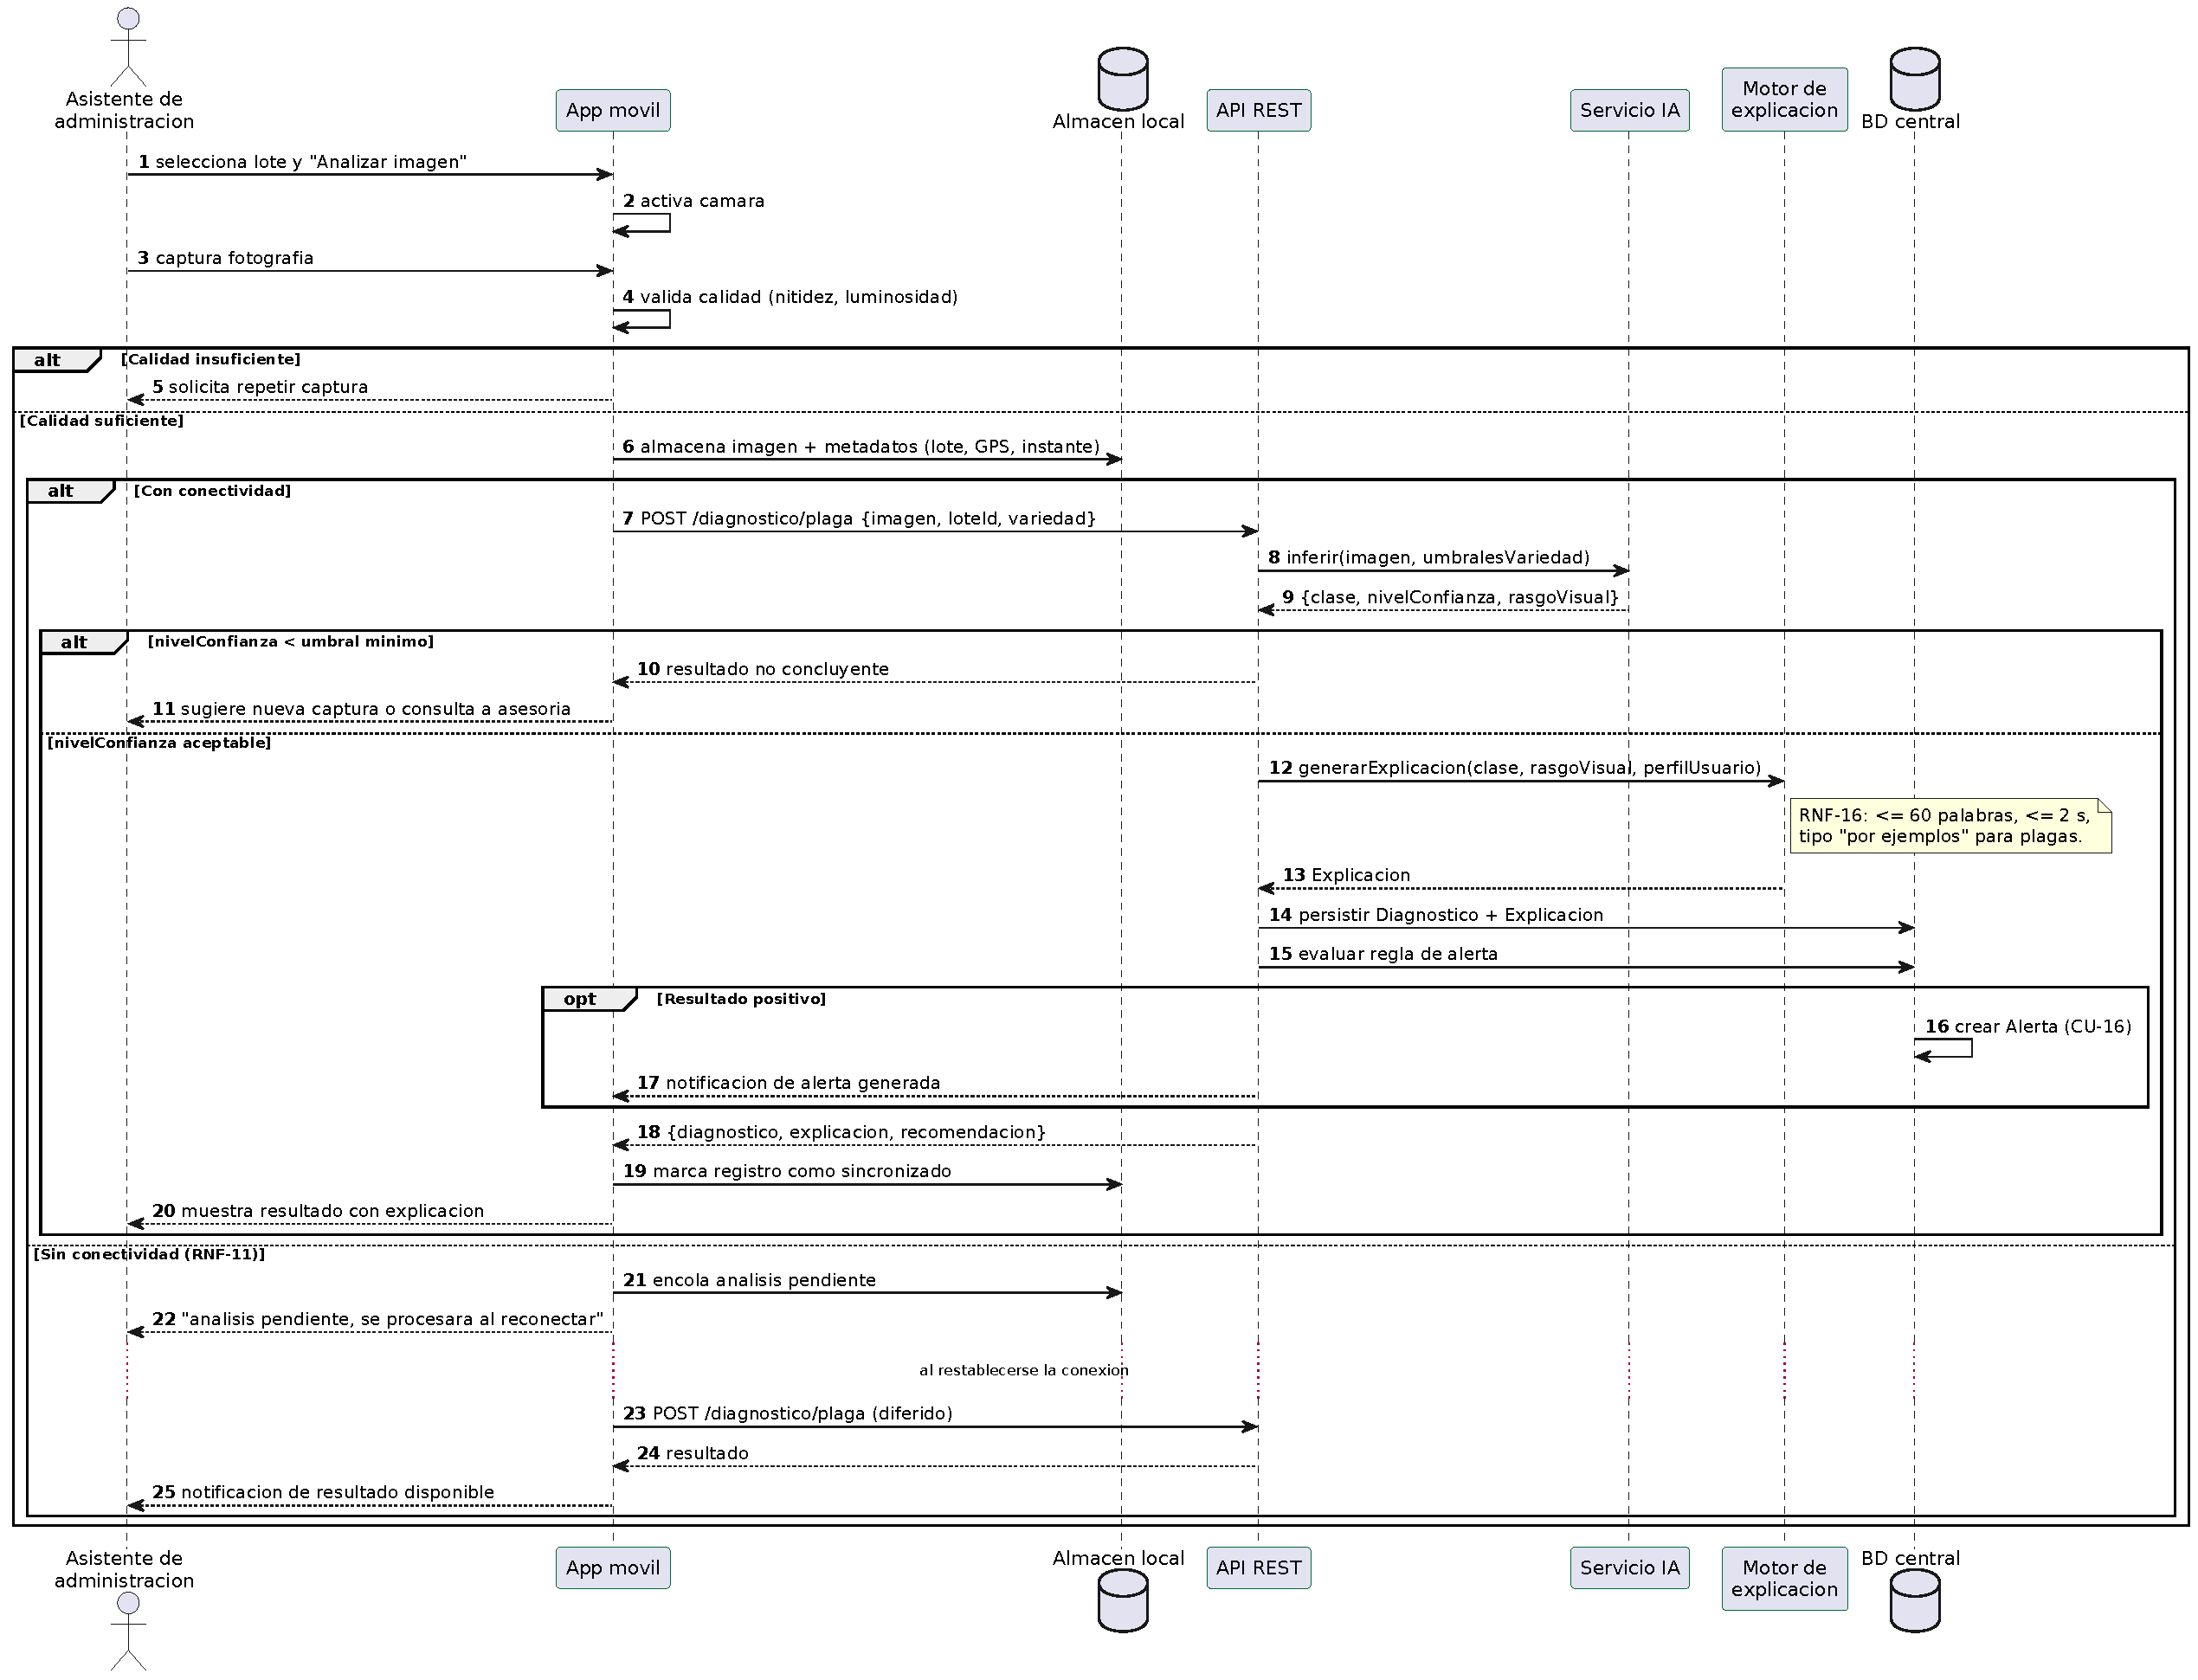
\includegraphics[width=1.0\textwidth]{img/secuencia_CU01}
\caption{Diagrama de secuencia del CU-01: análisis de imagen para detección de plaga, con las ramas de baja confianza y de operación sin conectividad.}
\label{fig:seq01}
\end{figure}

\begin{figure}[!htbp]
\centering
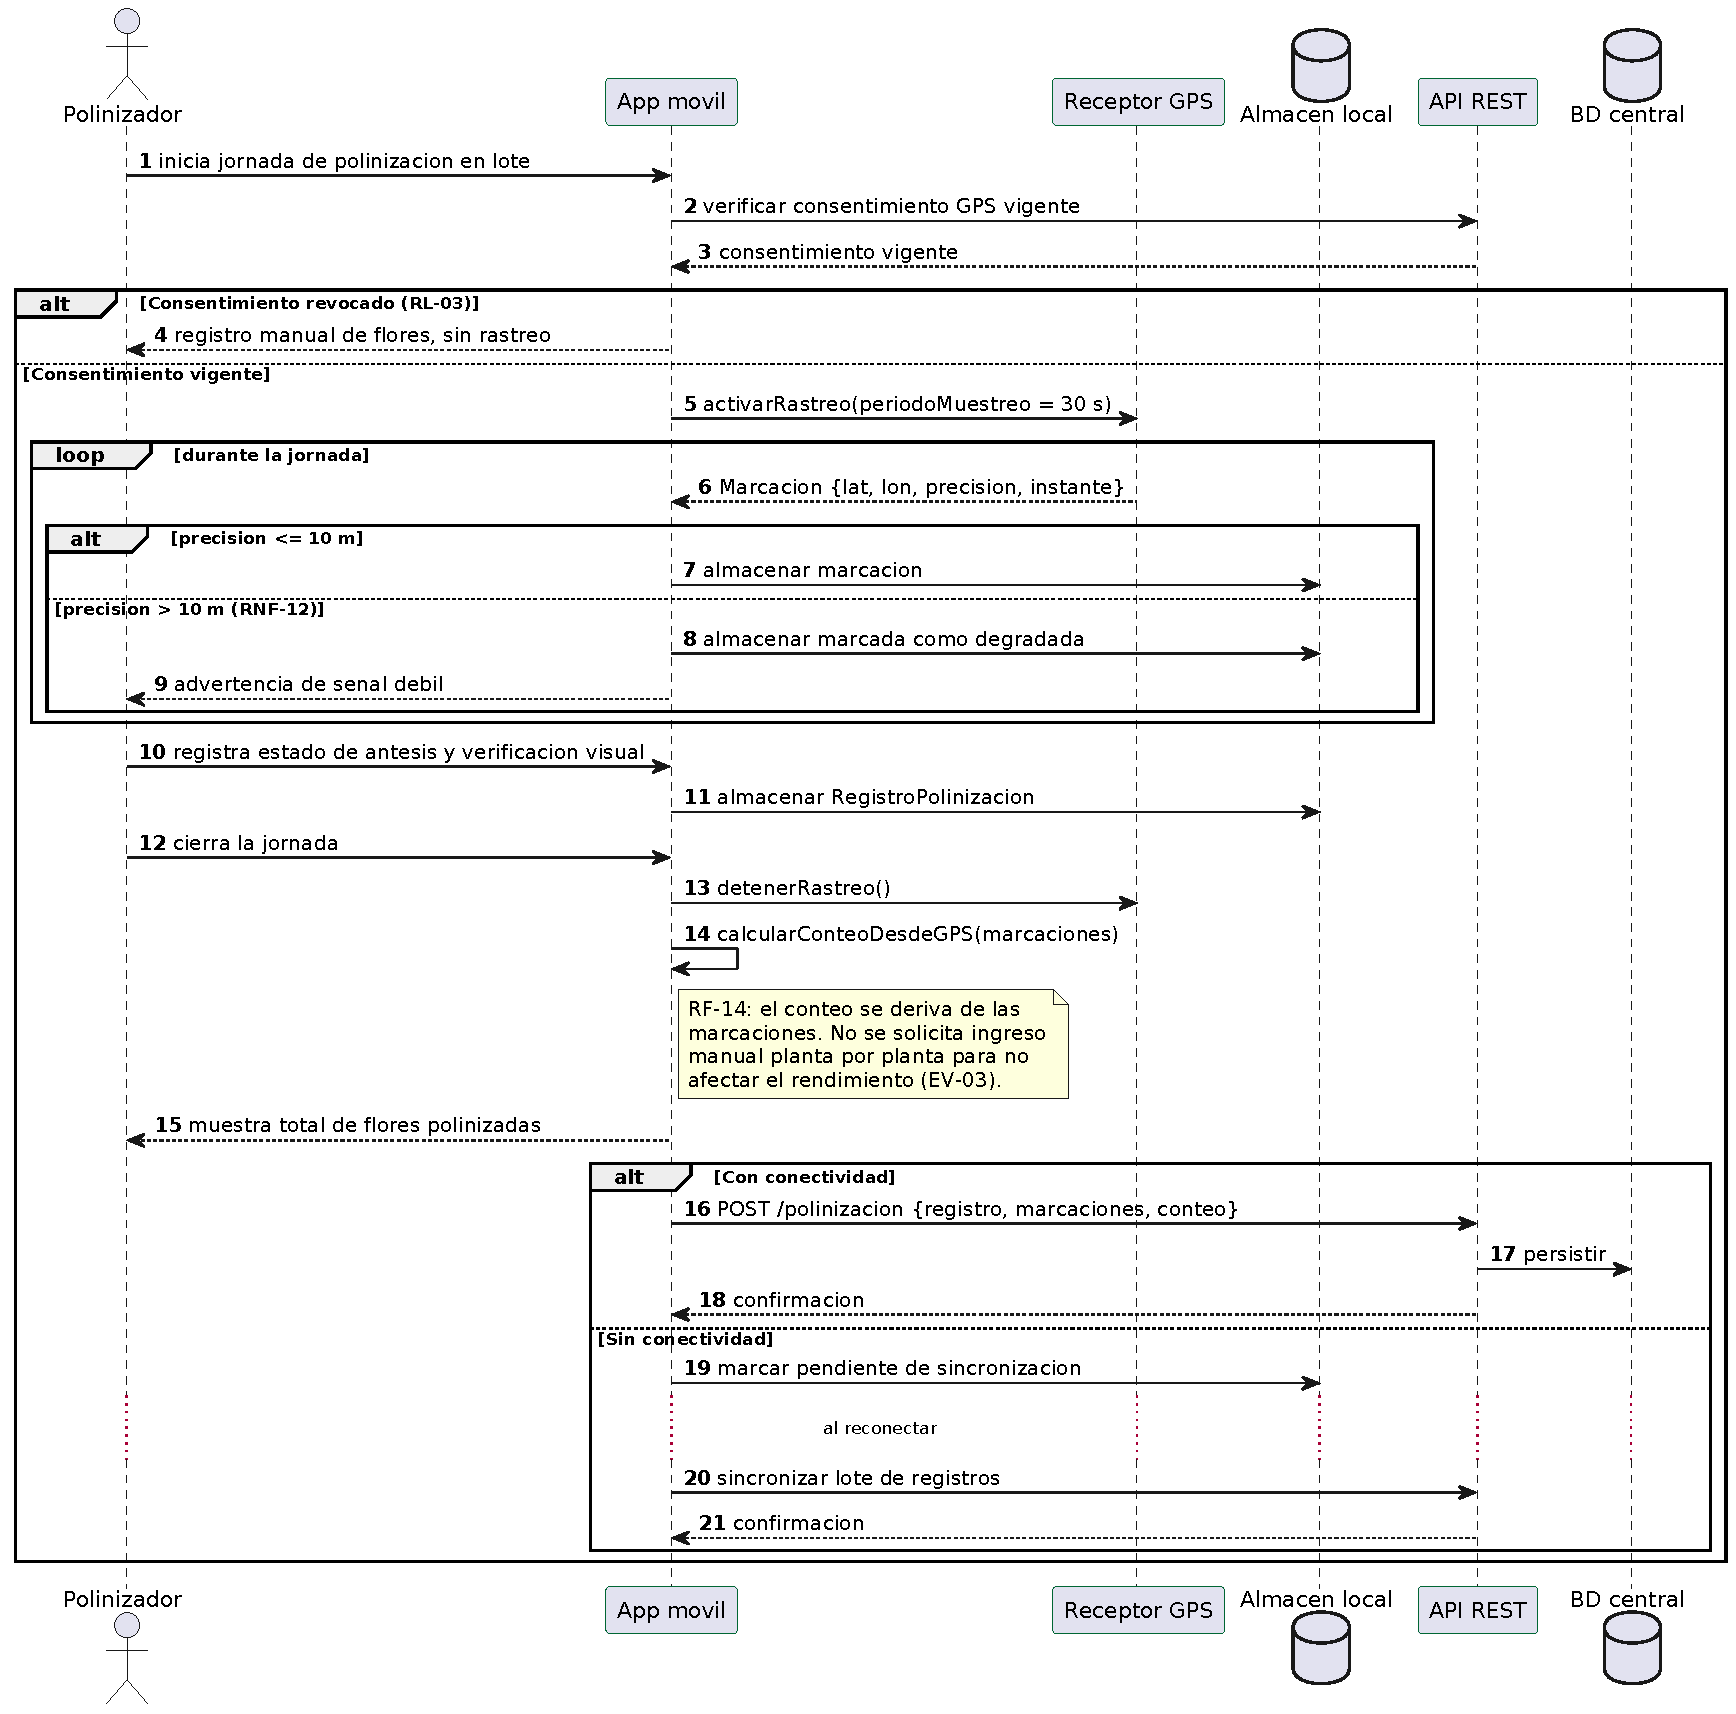
\includegraphics[width=1.0\textwidth]{img/secuencia_CU03}
\caption{Diagrama de secuencia del CU-03: registro de polinización y conteo georreferenciado, con verificación de consentimiento y manejo de precisión degradada.}
\label{fig:seq03}
\end{figure}

\begin{figure}[!htbp]
\centering
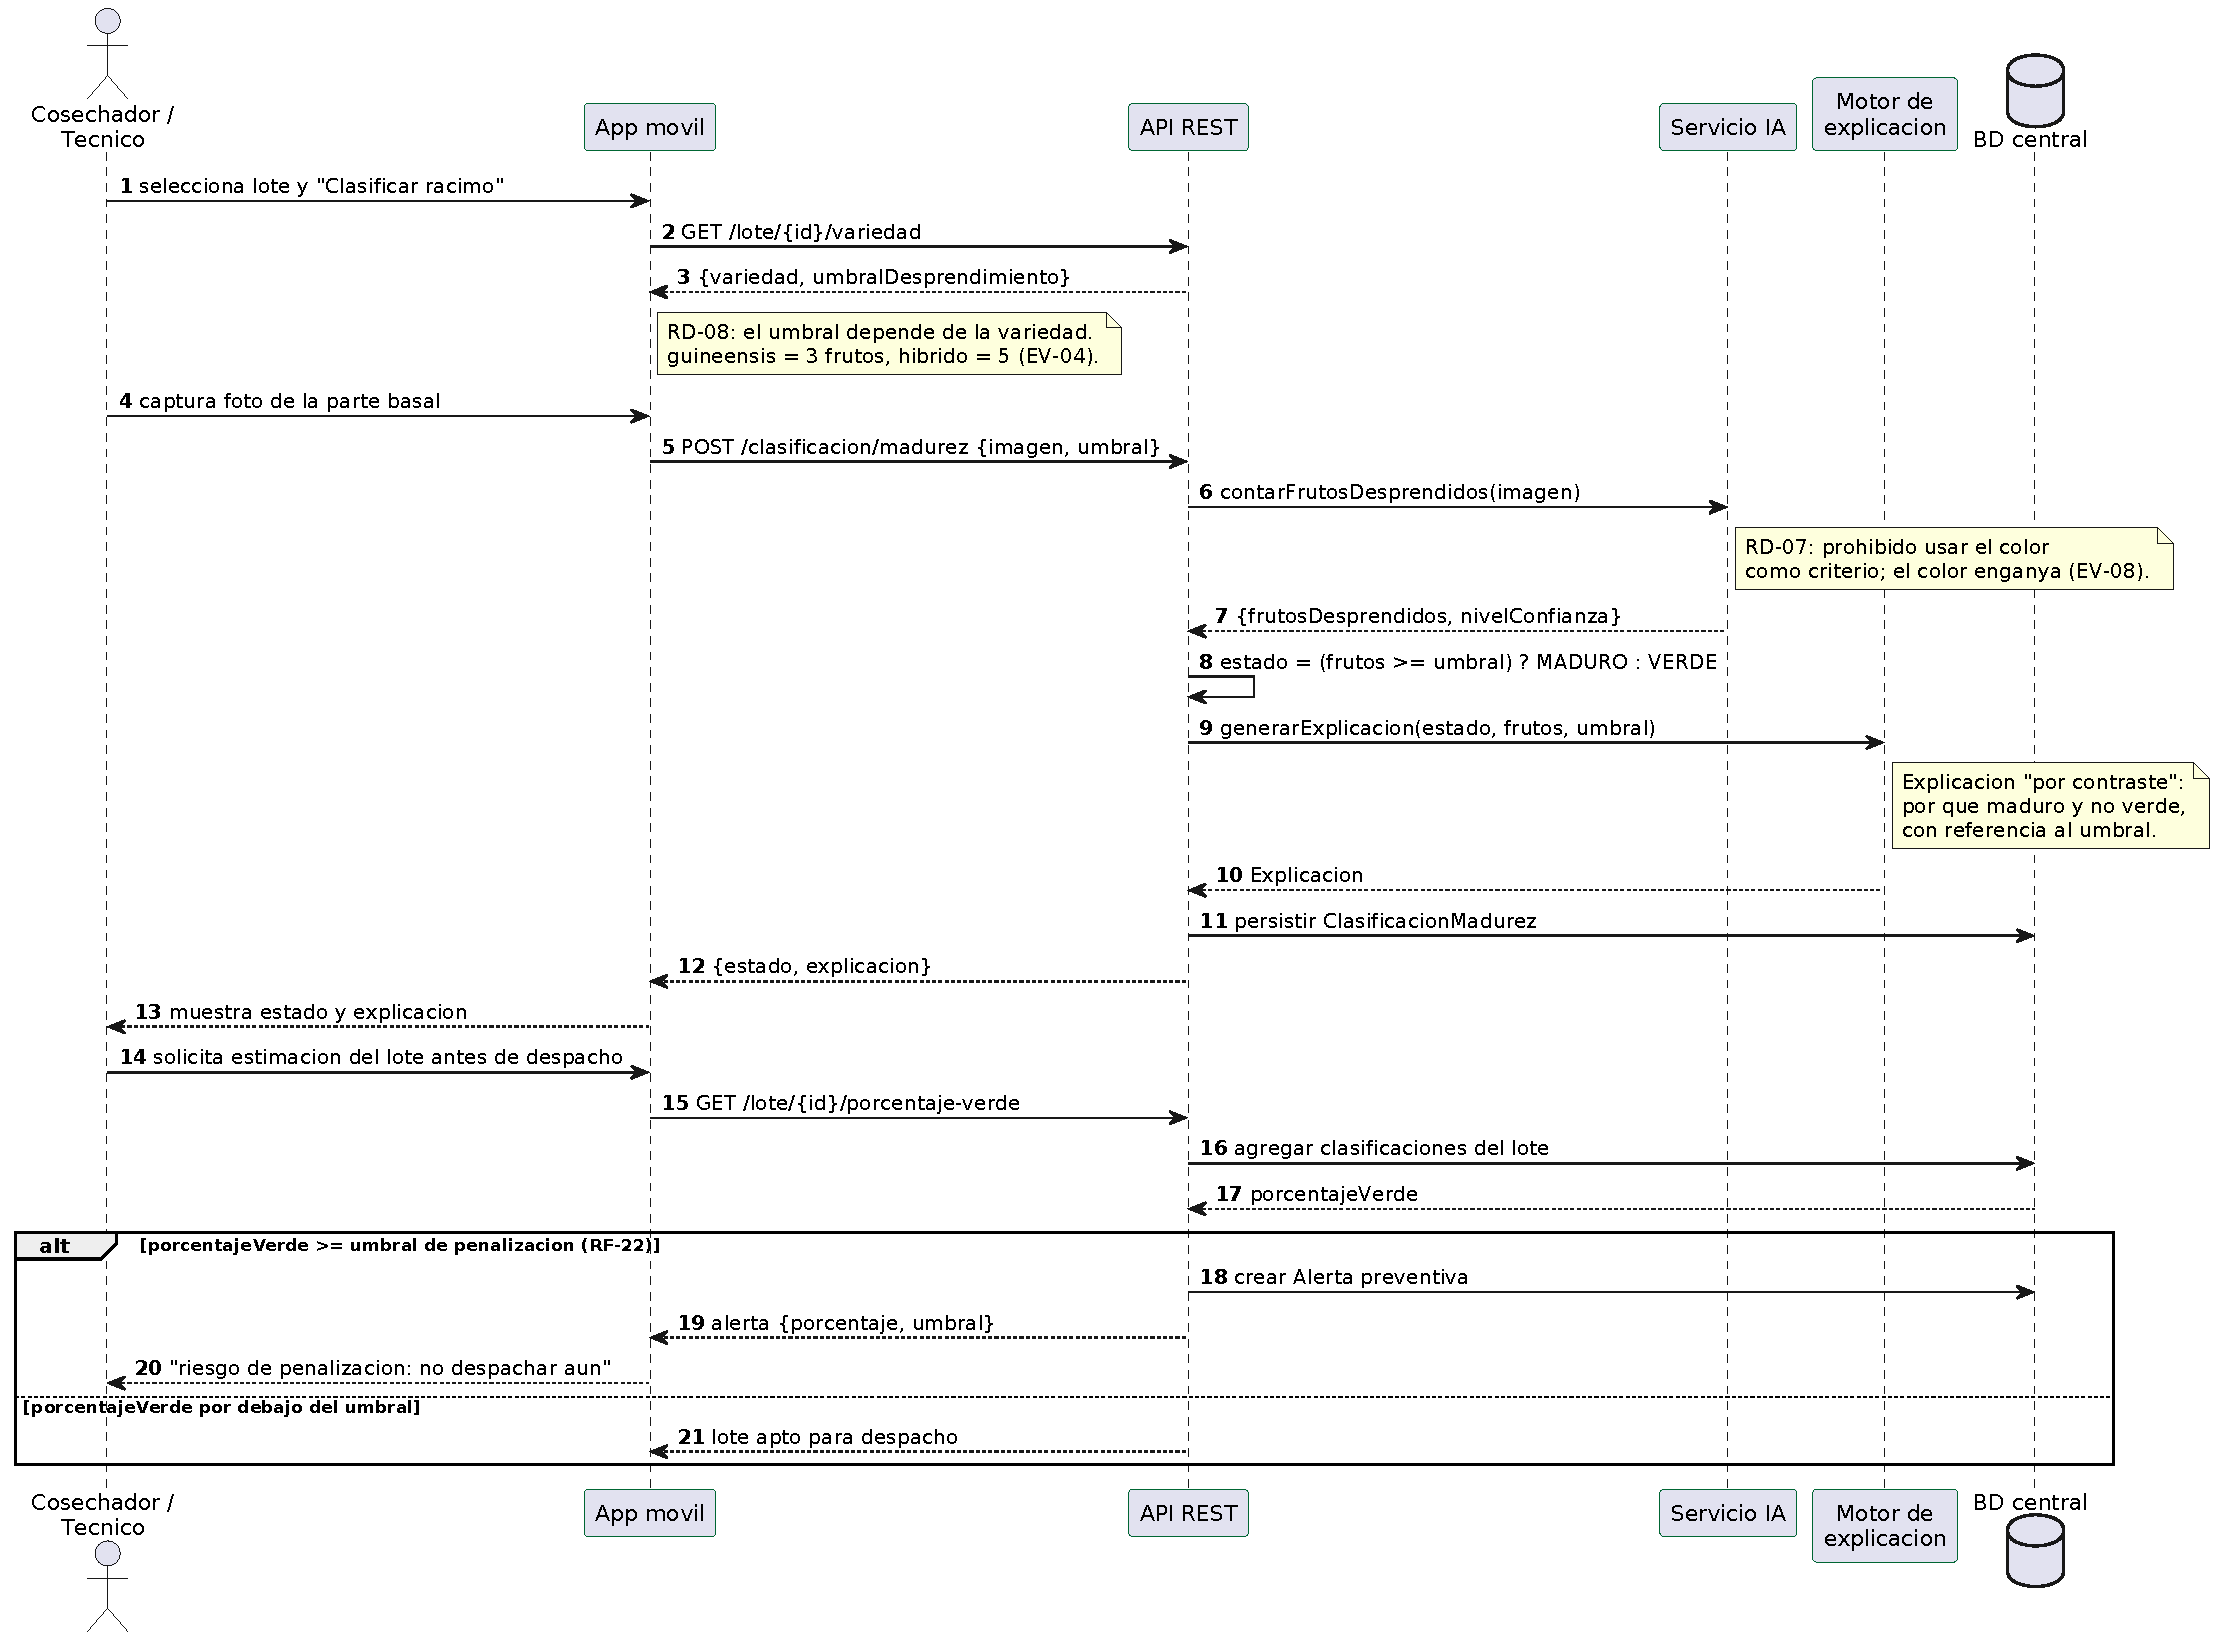
\includegraphics[width=1.0\textwidth]{img/secuencia_CU06}
\caption{Diagrama de secuencia del CU-06: clasificación de madurez del racimo y alerta preventiva de porcentaje de fruta verde.}
\label{fig:seq06}
\end{figure}

% ---------------------------------------------------------------------
\subsection{Diagrama de actividad}

El diagrama modela el ciclo semanal completo de planificación y ejecución, que constituye el proceso
central de la organización según los documentos operativos (\id{EV-11}). Incorpora la bifurcación
por disponibilidad de dispositivo (\id{RF-35}), la bifurcación por conectividad (\id{RNF-11}) y el
mecanismo de arrastre de labor incompleta (\id{RF-27}).

\begin{figure}[!htbp]
\centering
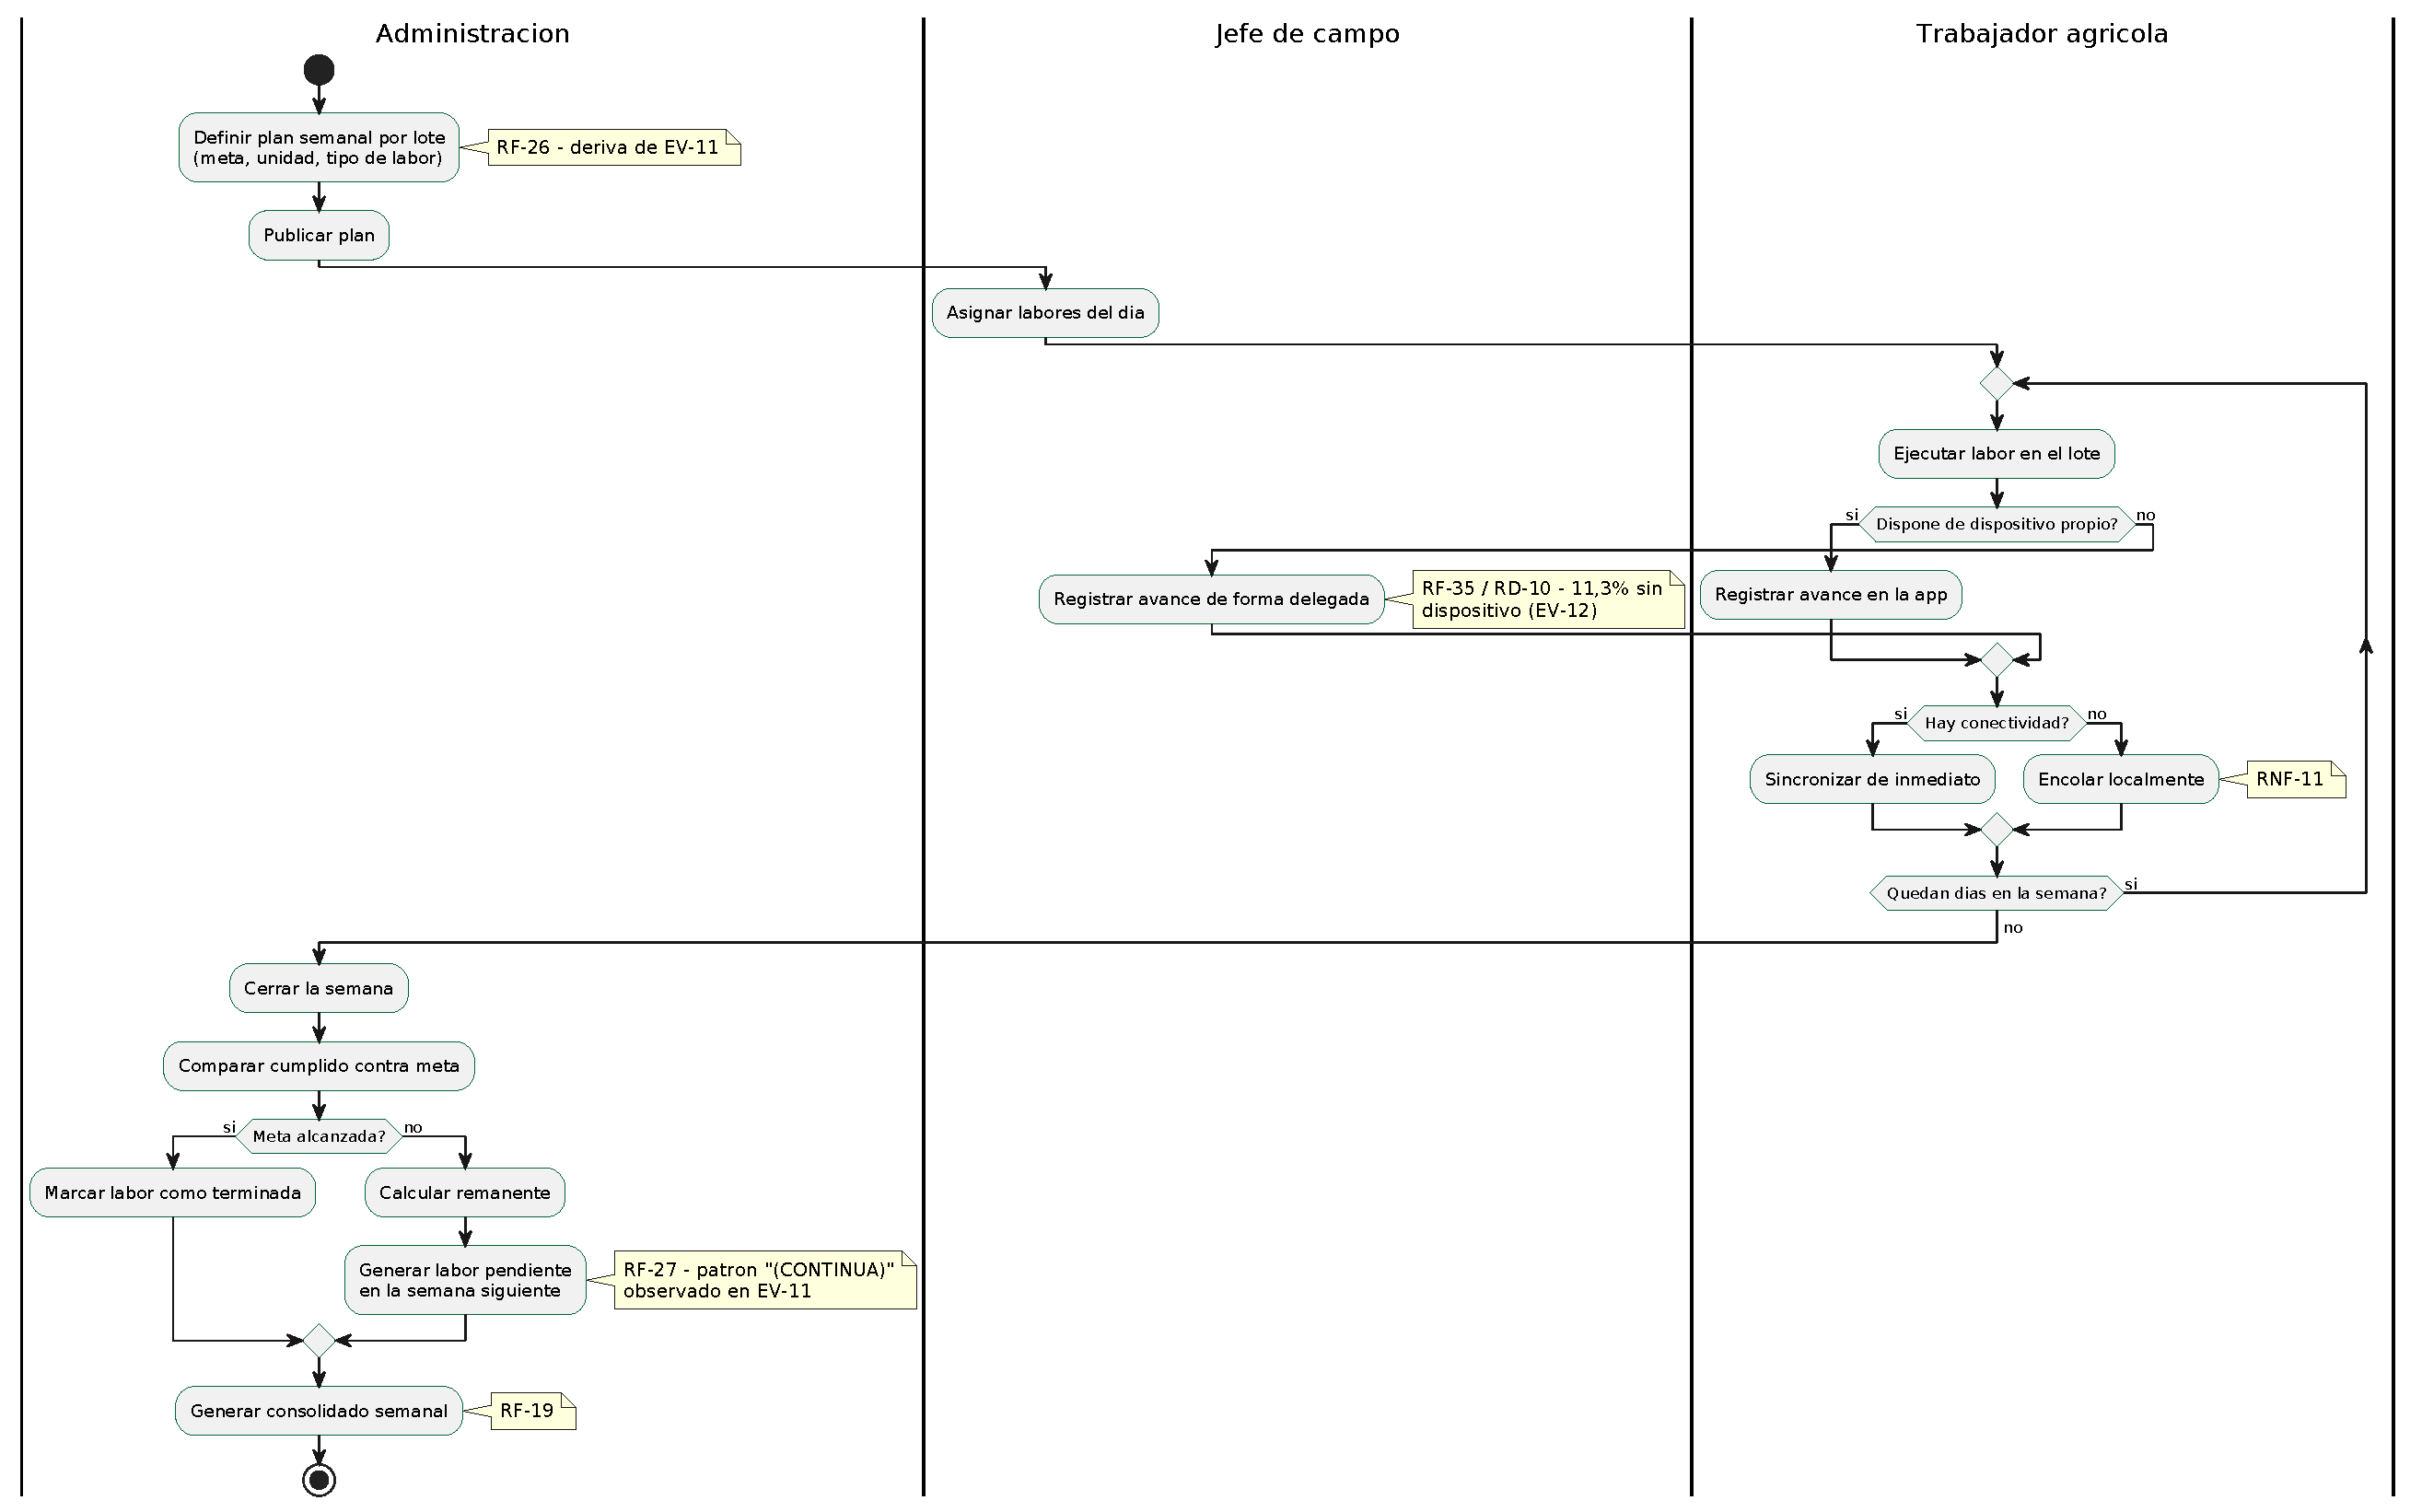
\includegraphics[width=1.0\textwidth]{img/actividad_ciclo_semanal}
\caption{Diagrama de actividad del ciclo semanal de planificación y ejecución de labores.}
\label{fig:actividad}
\end{figure}

% ---------------------------------------------------------------------
\subsection{Diagramas de estados}

Se modelan las dos entidades del dominio con ciclo de vida no trivial: el \textbf{racimo}, cuya
trayectoria determina el valor económico de la producción, y la \textbf{alerta}, cuyo ciclo refleja
la latencia real de verificación documentada en \id{EV-07}.

\begin{figure}[!htbp]
\centering
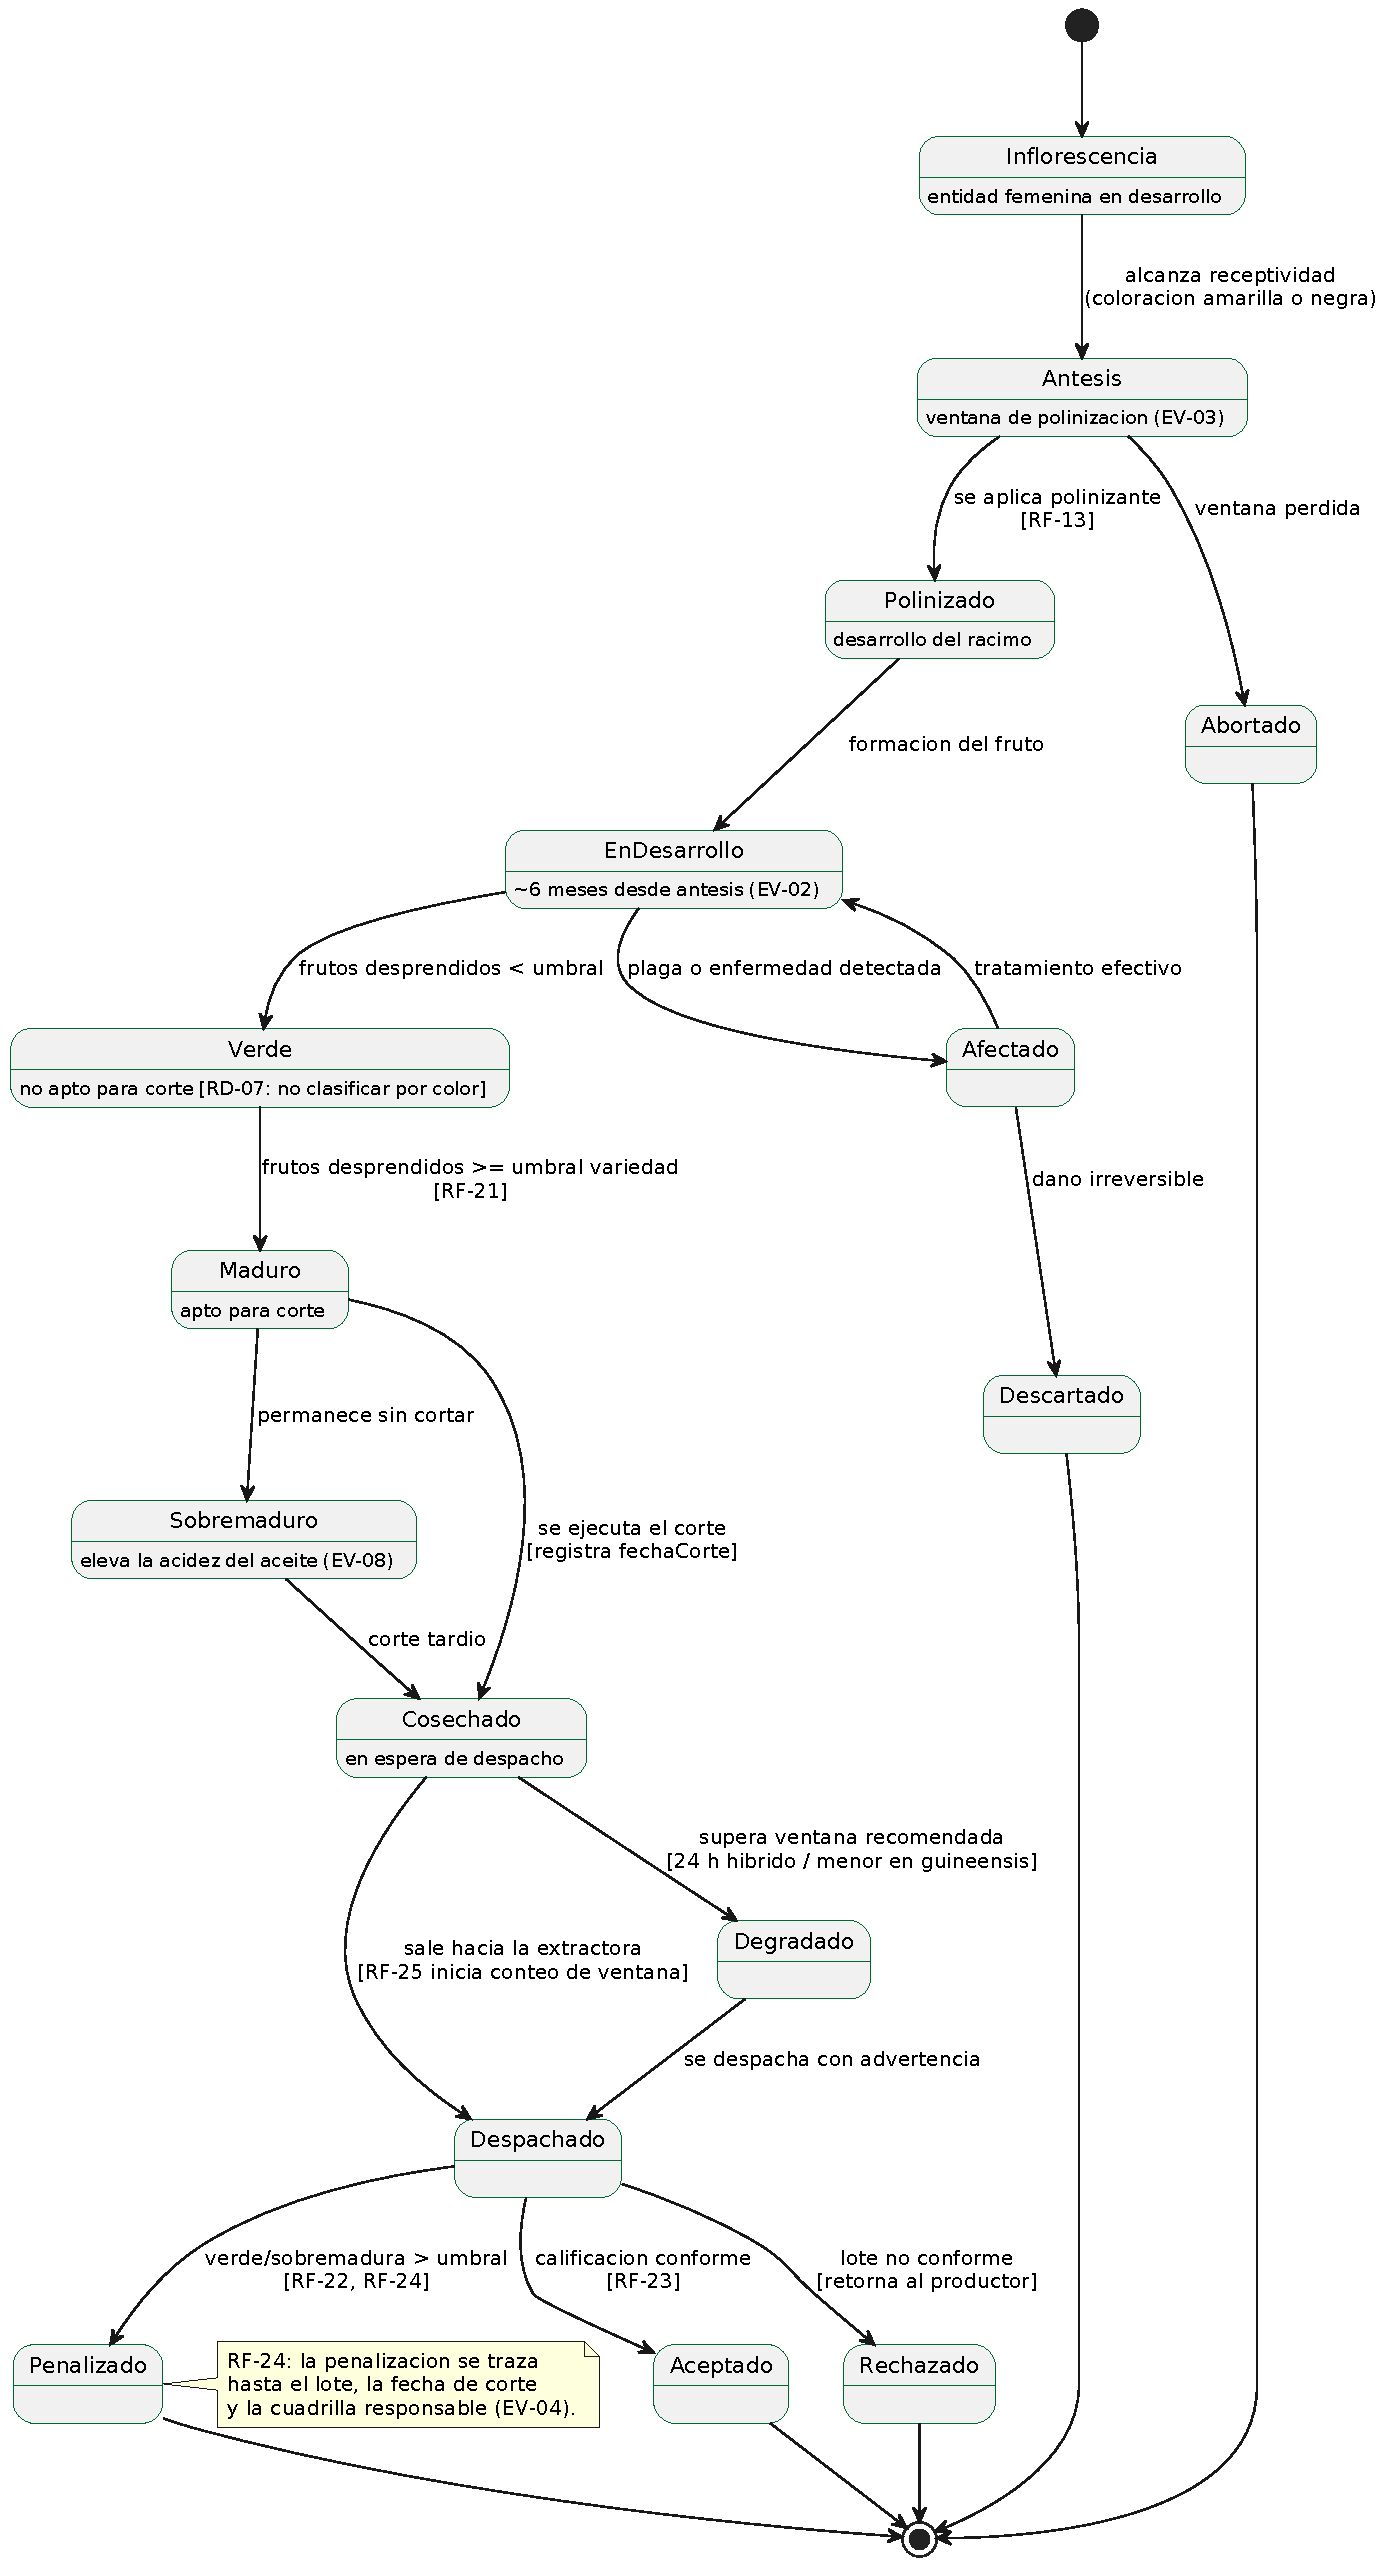
\includegraphics[width=0.67\textwidth]{img/estados_racimo}
\caption{Diagrama de estados del racimo, desde la inflorescencia hasta la calificación en la planta extractora.}
\label{fig:est_racimo}
\end{figure}

\begin{figure}[!htbp]
\centering
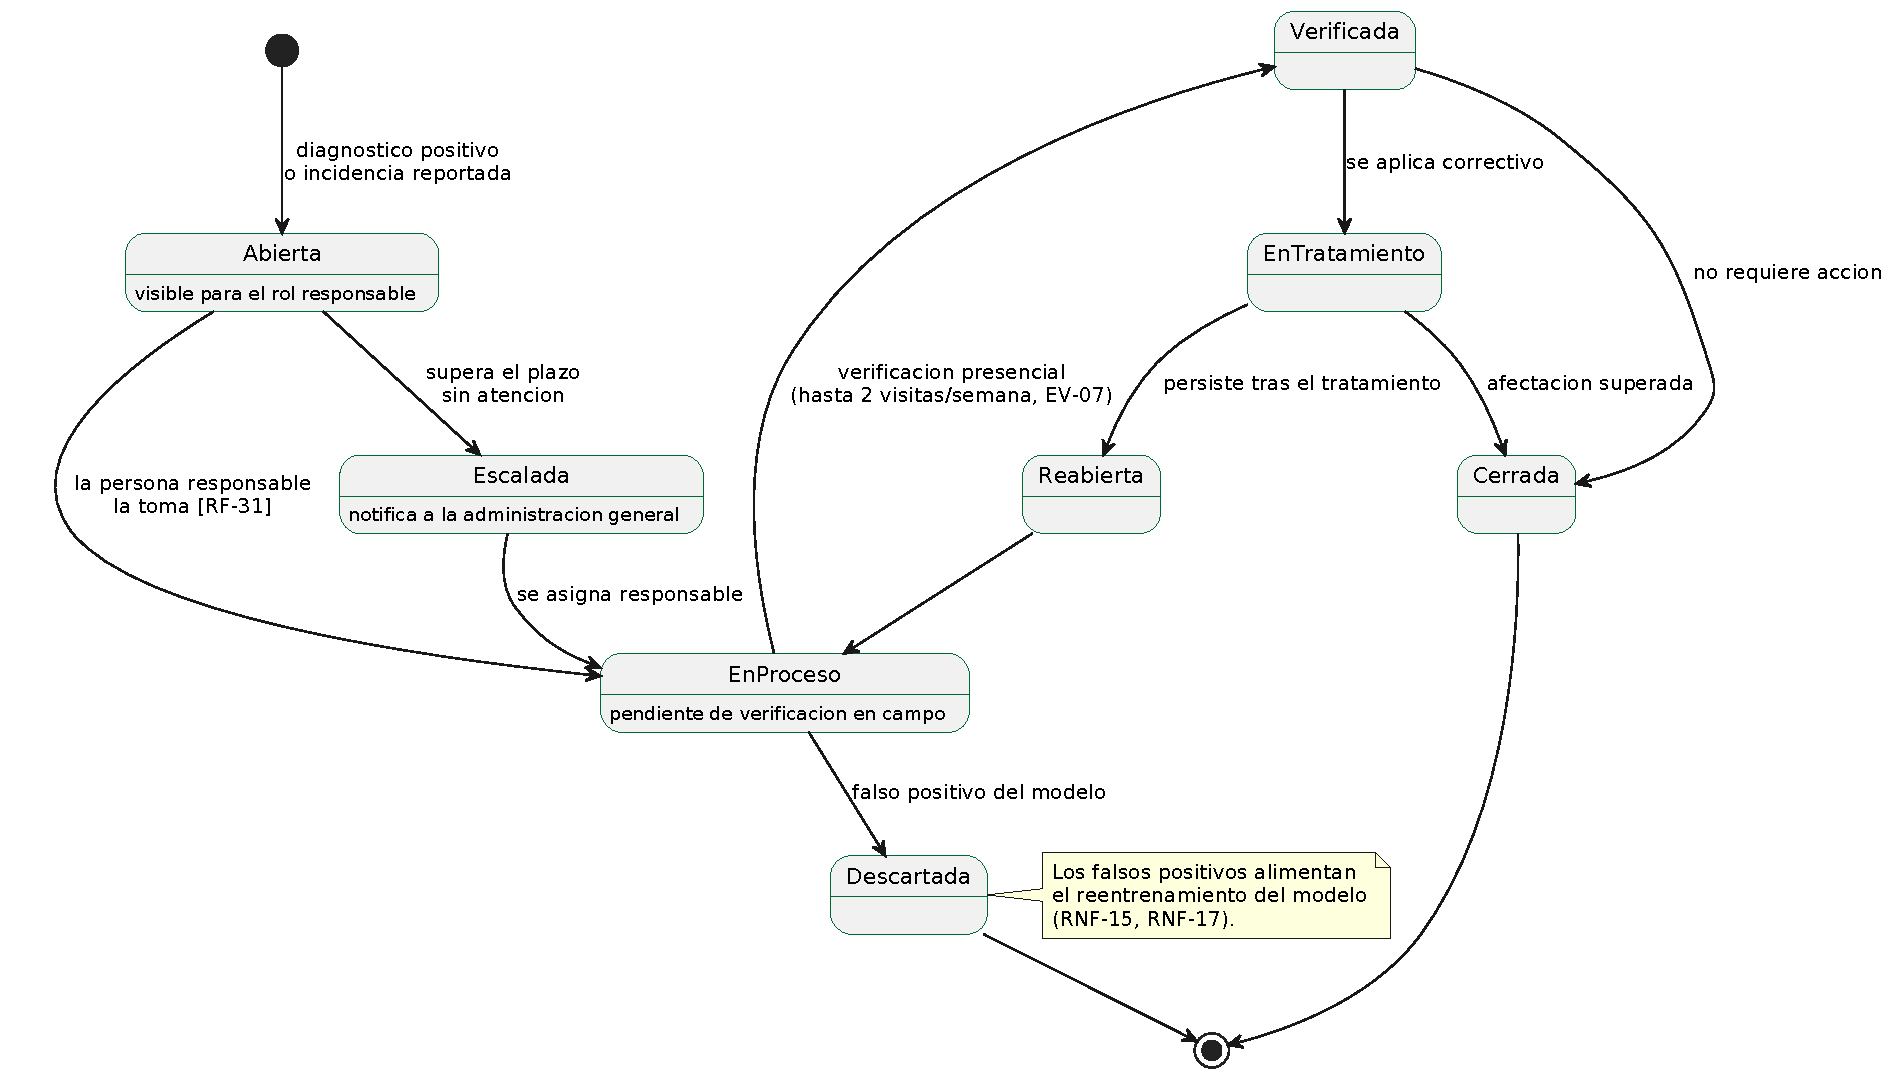
\includegraphics[width=1.0\textwidth]{img/estados_alerta}
\caption{Diagrama de estados de la alerta, con escalamiento por vencimiento de plazo y reapertura tras tratamiento inefectivo.}
\label{fig:est_alerta}
\end{figure}

\noindent
El estado \emph{Degradado} del racimo materializa el hallazgo de \id{EV-04} sobre la ventana entre
corte y entrega: el material híbrido tolera un intervalo mayor por su contenido de antioxidantes,
mientras que el \emph{guineensis} se deshidrata en dos o tres días. El estado \emph{Descartada} de
la alerta corresponde a los falsos positivos del modelo y alimenta el ciclo de reentrenamiento
previsto en \id{RNF-15} y \id{RNF-17}.

% ---------------------------------------------------------------------
\subsection{Diagrama de componentes}

\begin{figure}[!htbp]
\centering
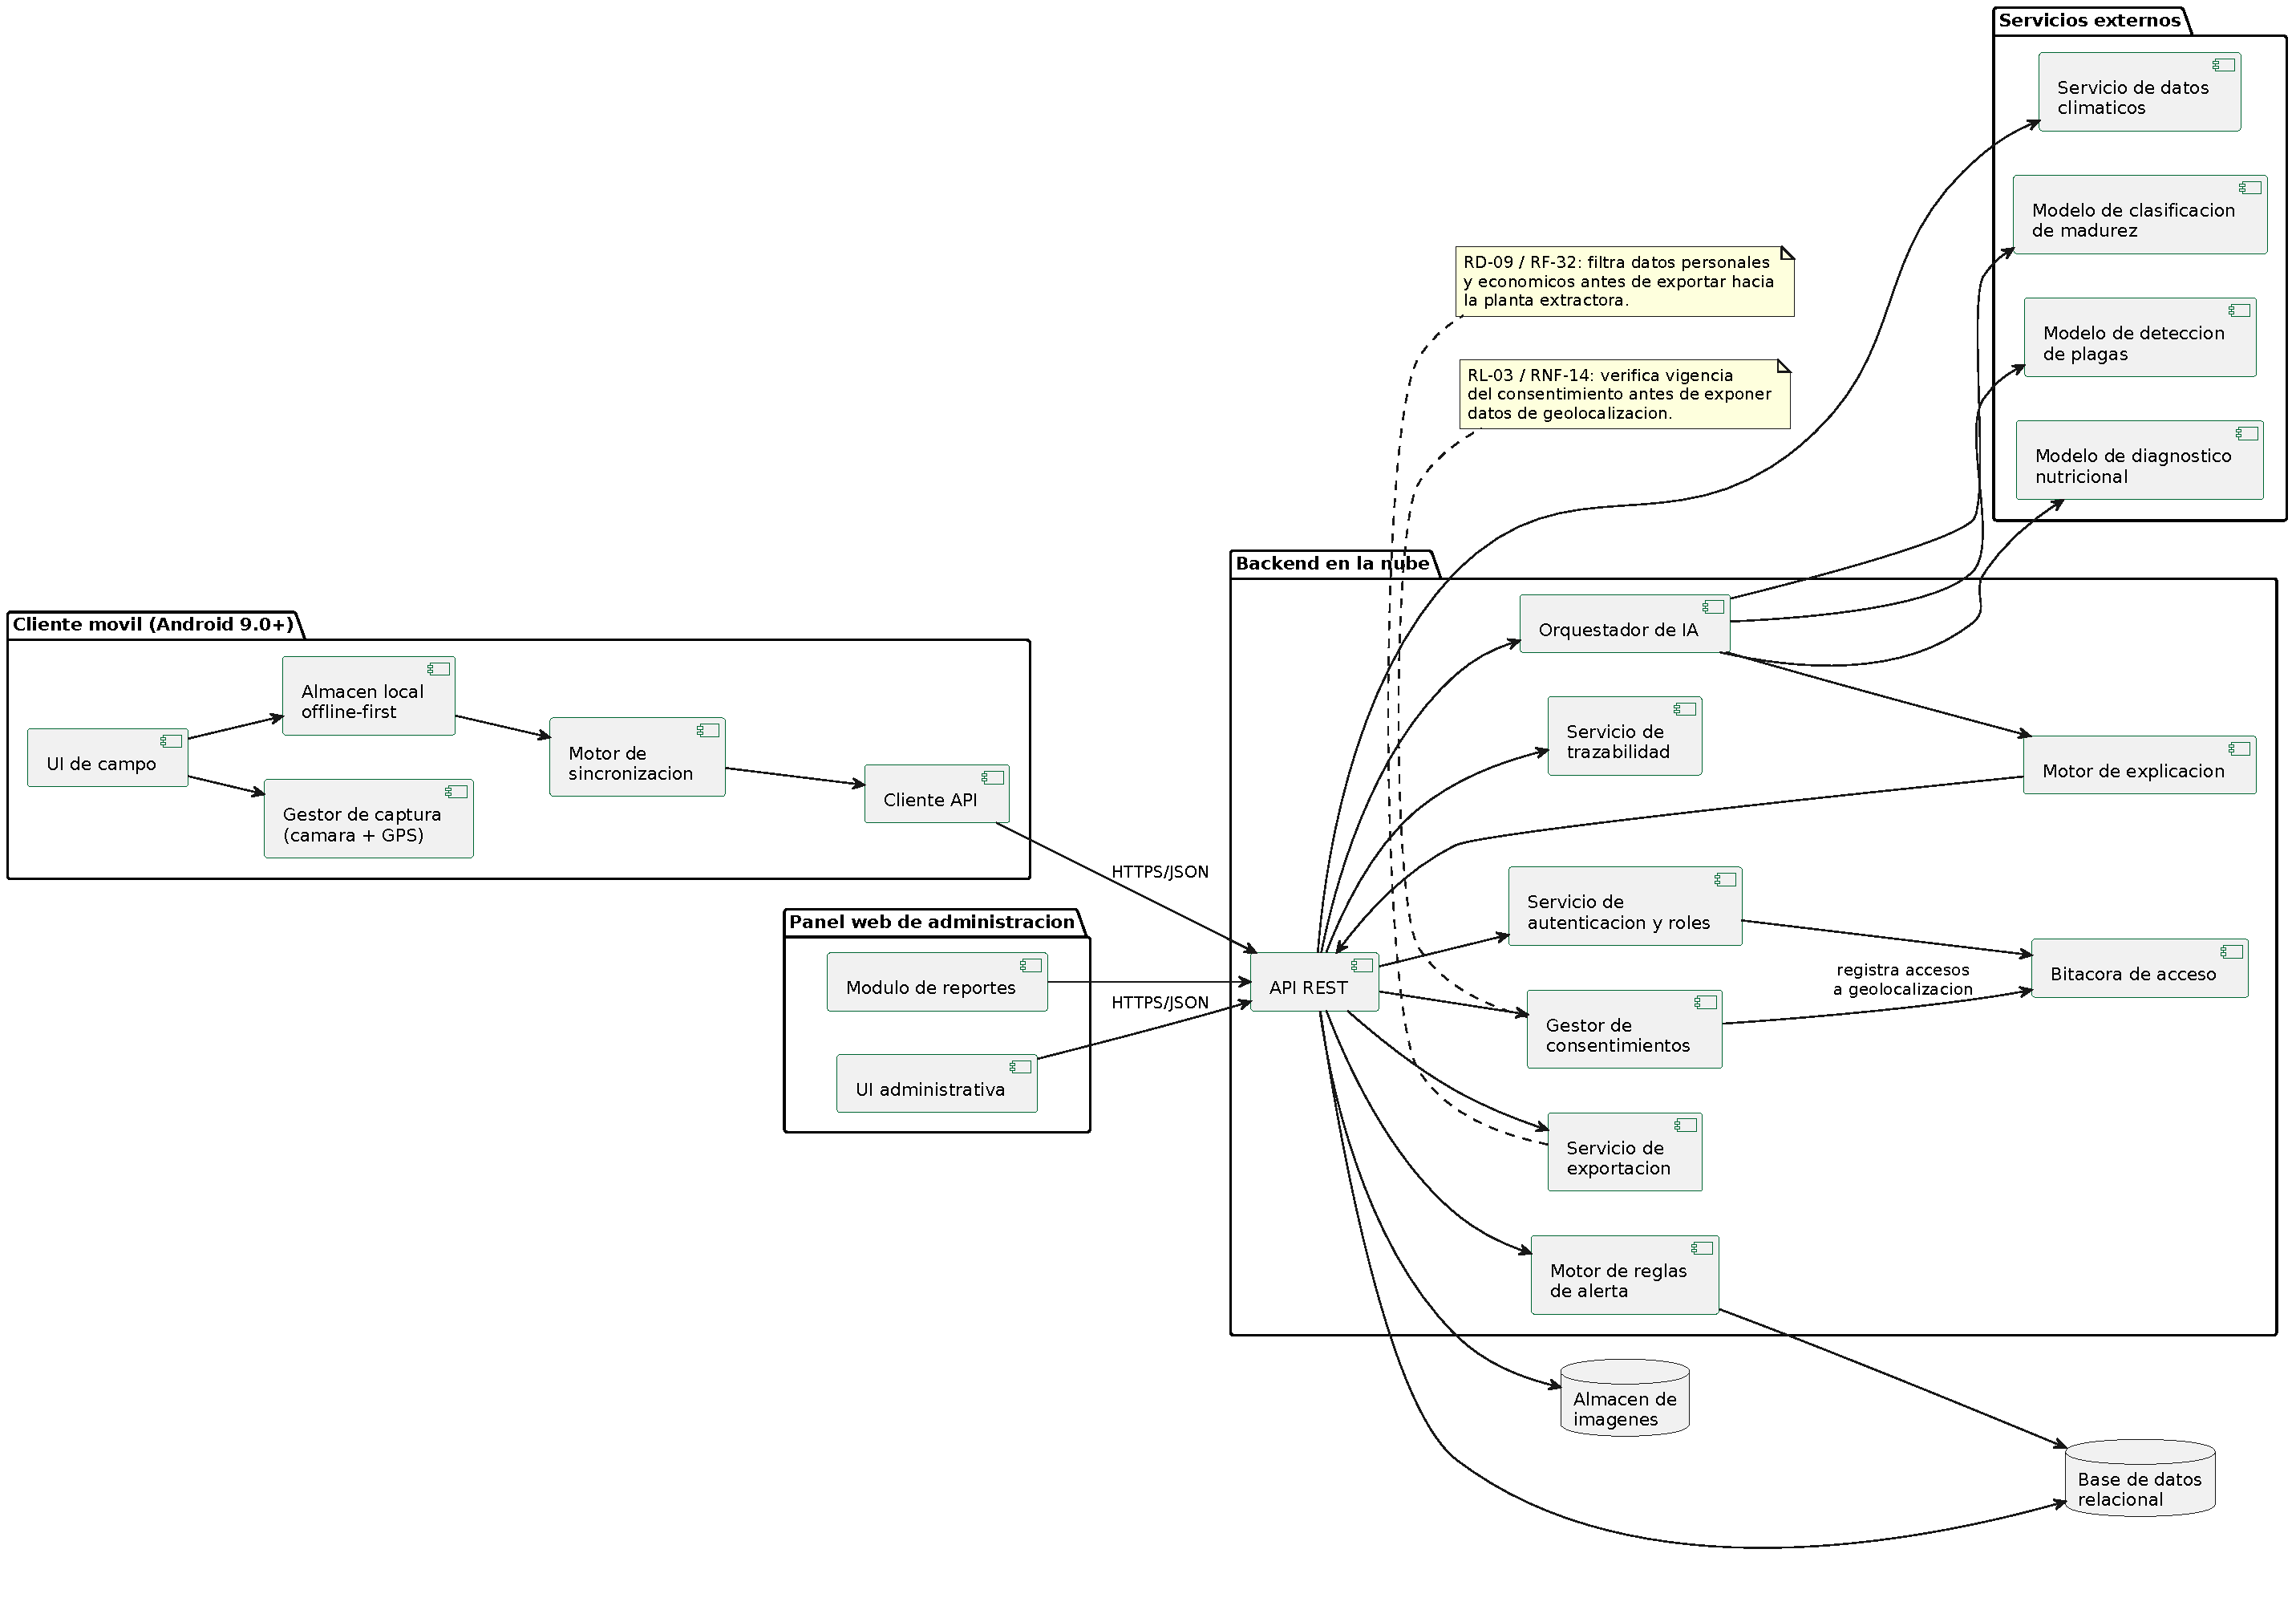
\includegraphics[width=1.0\textwidth]{img/componentes}
\caption{Diagrama de componentes del SIMPA.}
\label{fig:componentes}
\end{figure}

\noindent
Dos componentes merecen mención explícita por su origen normativo. El \emph{gestor de
consentimientos} verifica la vigencia antes de exponer cualquier dato de geolocalización y registra
todo acceso en la bitácora (\id{RL-03}, \id{RNF-14}). El \emph{servicio de exportación} filtra los
datos personales y económicos antes de generar el archivo destinado a la planta extractora
(\id{RD-09}, \id{RF-32}); su existencia como componente separado responde al criterio expreso de la
contraparte de que hay información que no puede compartirse (\id{EV-04}).

% ---------------------------------------------------------------------
\subsection{Diagrama de despliegue}

\begin{figure}[!htbp]
\centering
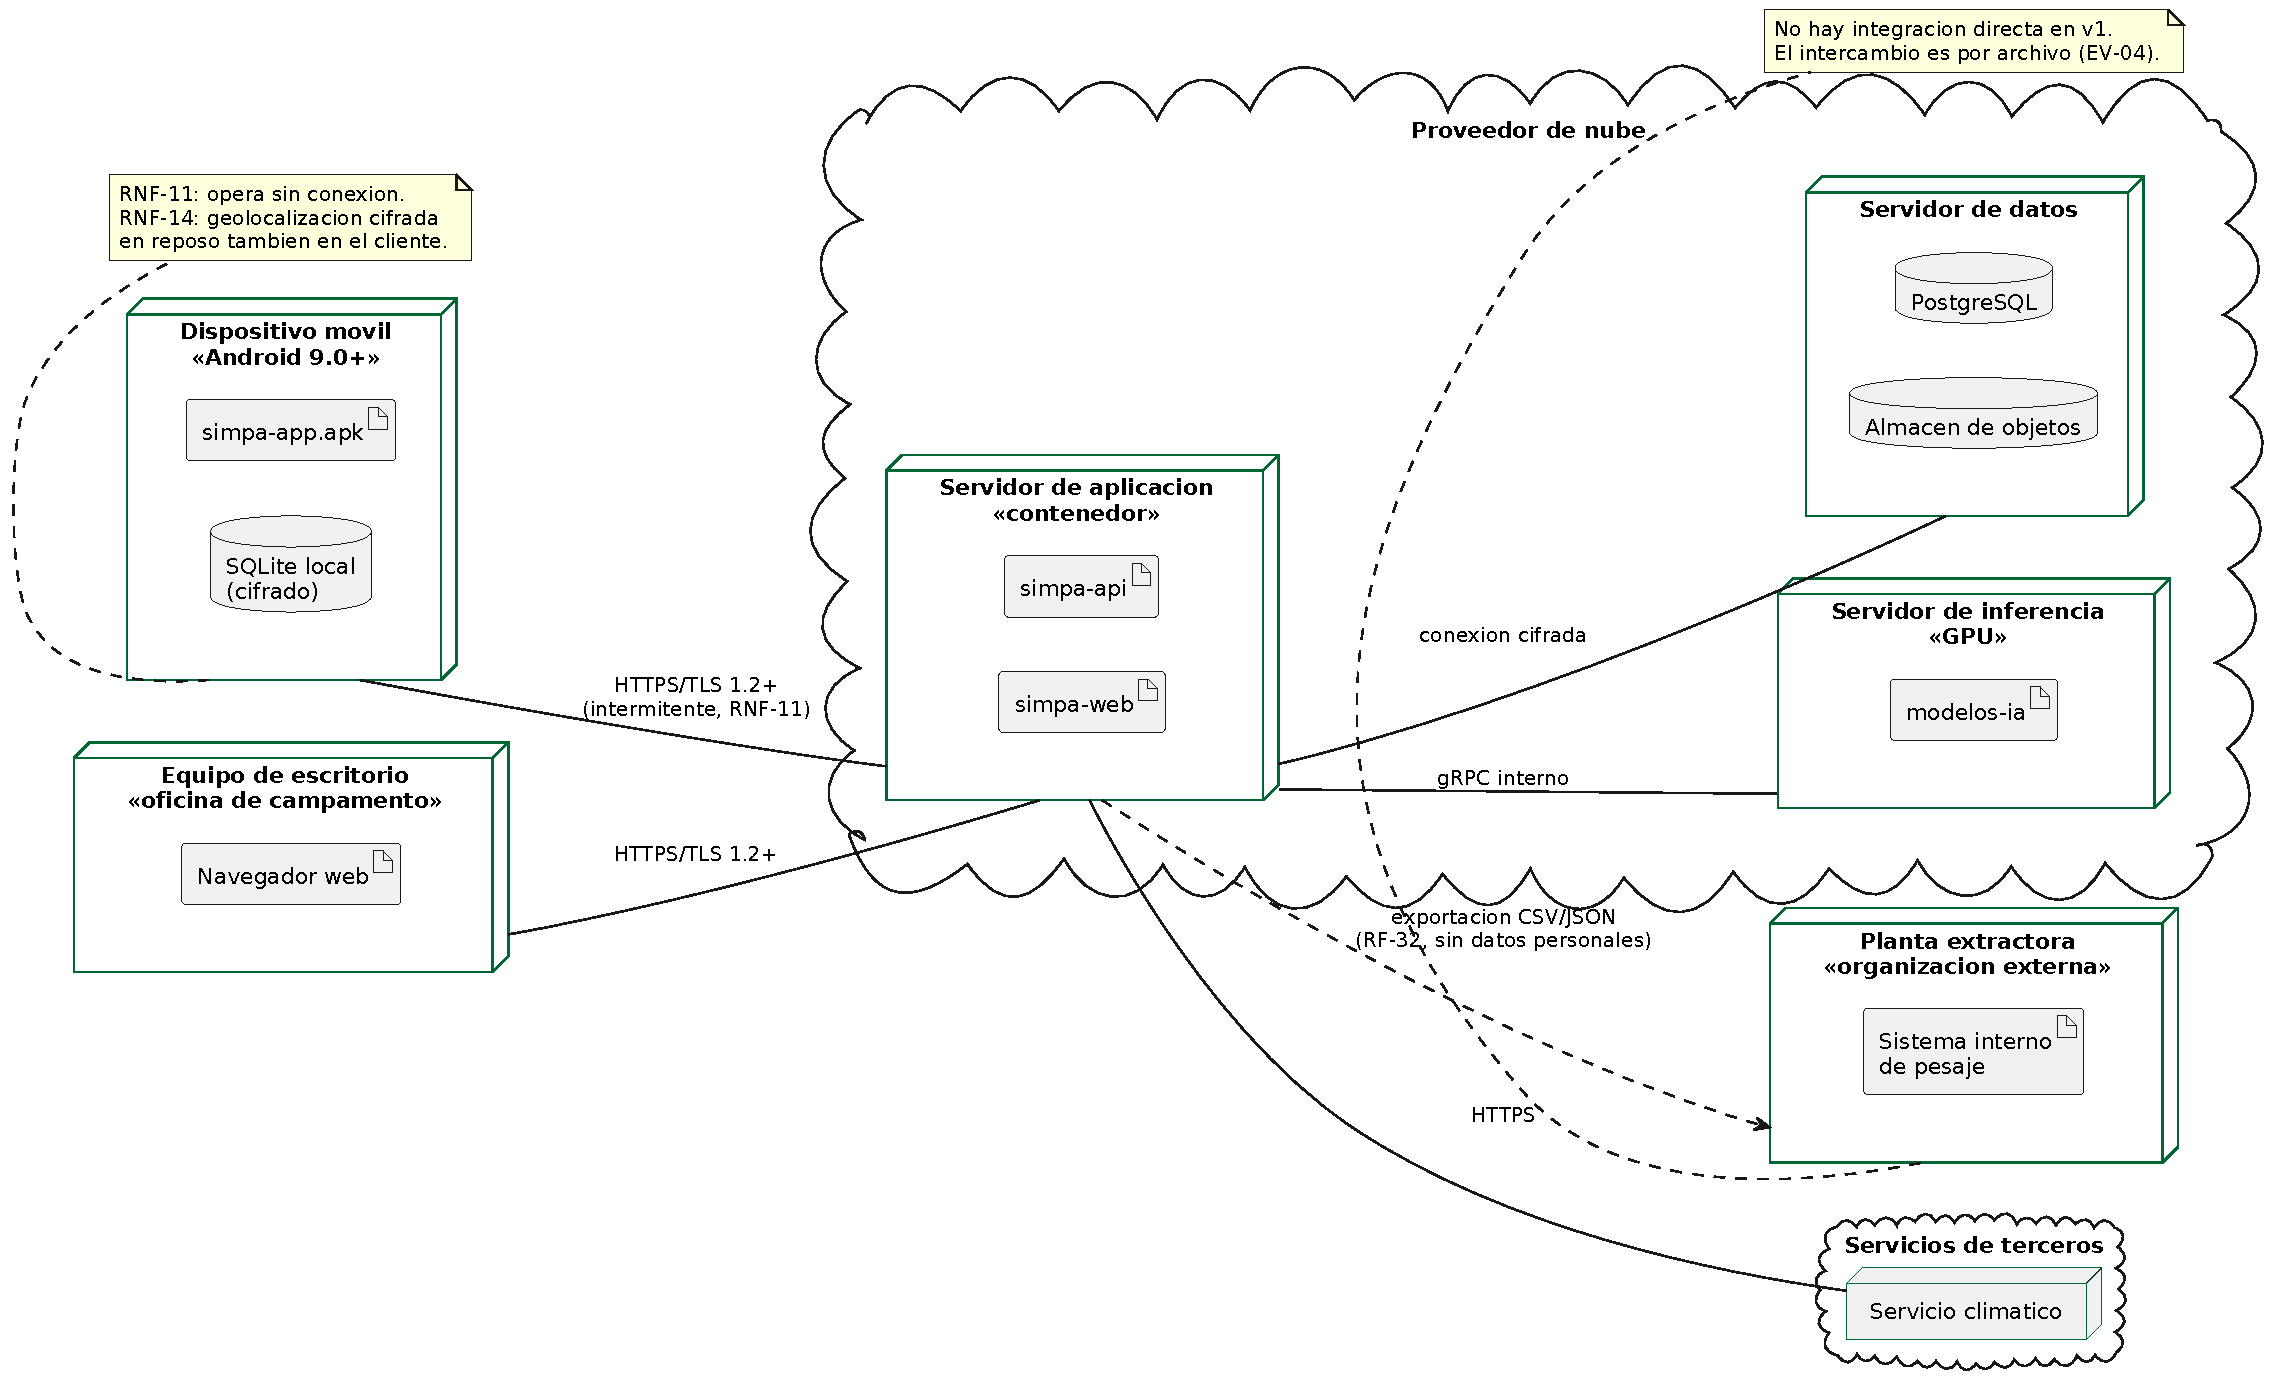
\includegraphics[width=1.0\textwidth]{img/despliegue}
\caption{Diagrama de despliegue del SIMPA.}
\label{fig:despliegue}
\end{figure}

\noindent
El enlace entre el dispositivo móvil y el servidor de aplicación se declara explícitamente como
\emph{intermitente}: el 74{,}2\% de las personas destinatarias no dispone de conectividad permanente
(\id{EV-12}). La planta extractora se representa como nodo externo sin integración directa; el
intercambio en la versión v1 se realiza por archivo, conforme a \id{RF-32}.

% ---------------------------------------------------------------------
\subsection{Cobertura del modelado}

\begin{longtable}{|L{4.6cm}|C{2.2cm}|C{2.2cm}|L{5.0cm}|}
\hline
\rowcolor{grisclaro}\textbf{Artefacto} & \textbf{Exigido} & \textbf{Entregado} & \textbf{Observación} \\
\hline
\endhead
Diagrama de casos de uso general & 1 & 1 & 8 actores, 18 casos de uso \\ \hline
Casos de uso detallados & 10 & 10 & Todos los \emph{Must}; $\geq 2$ flujos alternativos y $\geq 1$ excepción cada uno \\ \hline
Diagrama de clases refinado & 1 & 1 & 25 clases con atributos y operaciones \\ \hline
Diagramas de secuencia & CU \emph{Must} & 3 & CU-01, CU-03, CU-06 \\ \hline
Diagramas de actividad & Flujos principales & 1 & Ciclo semanal completo \\ \hline
Diagramas de estados & Entidades no triviales & 2 & Racimo y Alerta \\ \hline
Diagrama de componentes & 1 & 1 & --- \\ \hline
Diagrama de despliegue & 1 & 1 & --- \\ \hline
\caption{Cobertura del modelado UML frente a lo exigido en la §3.4 de la guía}
\end{longtable}
